% ******************************* PhD Thesis Template **************************
% Please have a look at the README.md file for info on how to use the template

\documentclass[a4paper,12pt,authoryear,index,print]{common/PhDThesisPSnPDF}

%\usepackage{draftwatermark}
%\SetWatermarkLightness{0.95}

% ******************************************************************************
% ****************************** Custom Margin *********************************

% Add `custommargin' in the document class options to use this section
% Set {innerside margin / outerside margin / topmargin / bottom margin}  and
% other page dimensions

\ifsetMargin
\else
    \RequirePackage[left=37mm,right=30mm,top=35mm,bottom=30mm]{geometry}
    \setFancyHdr % To apply fancy header after geometry package is loaded
\fi


%\chead{Unfinished draft}
%\cfoot{\texttt{Unfinished draft - compiled on \today{} at \currenttime}}

% *****************************************************************************
% ******************* Fonts (like different typewriter fonts etc.)*************

% Add `customfont' in the document class option to use this section

\ifsetFont
\else
    % Set your custom font here and use `customfont' in options. Leave empty to
    % load computer modern font (default LaTeX font).  

    \RequirePackage{libertine} 
\fi

% *****************************************************************************
% *************************** Bibliography  and References ********************

%\usepackage{cleveref} %Referencing without need to explicitly state fig /table

% Add `custombib' in the document class option to use this section
\ifsetBib % True, Bibliography option is chosen in class options
\else % If custom bibliography style chosen then load bibstyle here

   \RequirePackage[square, sort, numbers, authoryear]{natbib} % CustomBib

% If you would like to use biblatex for your reference management, as opposed to the default `natbibpackage` pass the option `custombib` in the document class. Comment out the previous line to make sure you don't load the natbib package. Uncomment the following lines and specify the location of references.bib file

% \RequirePackage[backend=biber, style=numeric-comp, citestyle=numeric, sorting=nty, natbib=true]{biblatex}
% \bibliography{References/references} %Location of references.bib only for biblatex

\fi


% changes the default name `Bibliography` -> `References'
\renewcommand{\bibname}{References}


% *****************************************************************************
% *************** Changing the Visual Style of Chapter Headings ***************
% Uncomment the section below. Requires titlesec package.

%\RequirePackage{titlesec}
%\newcommand{\PreContentTitleFormat}{\titleformat{\chapter}[display]{\scshape\Large}
%{\Large\filleft{\chaptertitlename} \Huge\thechapter}
%{1ex}{}
%[\vspace{1ex}\titlerule]}
%\newcommand{\ContentTitleFormat}{\titleformat{\chapter}[display]{\scshape\huge}
%{\Large\filleft{\chaptertitlename} \Huge\thechapter}{1ex}
%{\titlerule\vspace{1ex}\filright}
%[\vspace{1ex}\titlerule]}
%\newcommand{\PostContentTitleFormat}{\PreContentTitleFormat}
%\PreContentTitleFormat


% *****************************************************************************
% **************************** Custom Packages ********************************
% *****************************************************************************


% ************************* Algorithms and Pseudocode **************************

%\usepackage{algpseudocode} 


% ********************Captions and Hyperreferencing / URL **********************

% Captions: This makes captions of figures use a boldfaced small font. 
%\RequirePackage[small,bf]{caption}

\RequirePackage[labelsep=space,tableposition=top]{caption} 
%\renewcommand{\figurename}{Figure} %to support older versions of captions.sty
\captionsetup{labelsep = colon,belowskip=12pt,aboveskip=4pt}

% ************************ Formatting / Footnote *******************************

%\usepackage[perpage]{footmisc} %Range of footnote options 


% ****************************** Line Numbers **********************************

%\RequirePackage{lineno}
%\linenumbers

% ************************** Graphics and figures *****************************

%\usepackage{rotating}
%\usepackage{wrapfig}
%\usepackage{float}
\usepackage{subfig} %note: subfig must be included after the `caption` package. 


% ********************************* Table **************************************

%\usepackage{longtable}
%\usepackage{multicol}
%\usepackage{multirow}
%\usepackage{tabularx}


% ***************************** Math and SI Units ******************************

\usepackage{amsfonts}
\usepackage{amsmath}
\usepackage{amssymb}
%\usepackage{siunitx} % use this package module for SI units


% ******************************************************************************
% ************************* User Defined Commands ******************************
% ******************************************************************************

% *********** To change the name of Table of Contents / LOF and LOT ************

%\renewcommand{\contentsname}{My Table of Contents}
%\renewcommand{\listfigurename}{List of figures}
%\renewcommand{\listtablename}{List of tables}


% ********************** TOC depth and numbering depth *************************

\setcounter{secnumdepth}{2}
\setcounter{tocdepth}{2}

% ******************************* Nomenclature *********************************

% To change the name of the Nomenclature section, uncomment the following line

%\renewcommand{\nomname}{Symbols}


% ********************************* Appendix ***********************************

% The default value of both \appendixtocname and \appendixpagename is `Appendices'. These names can all be changed via: 

%\renewcommand{\appendixtocname}{List of appendices}
%\renewcommand{\appendixname}{Appndx}

% All my custom preamble stuff.  Shouldn't overlap with anything in official-preamble




% Paths to figure and table directories.
\newcommand{\symmetryfigsdir}{figures/symmetries}
\newcommand{\topologyfiguresdir}{figures/topology}
\newcommand{\infinitefiguresdir}{figures/infinite}
\newcommand{\grammarfiguresdir}{figures/grammar}
\newcommand{\introfigsdir}{figures/intro}
\newcommand{\gplvmfiguresdir}{figures/gplvm}
\newcommand{\warpedfiguresdir}{figures/warped-mixtures}
\newcommand{\deeplimitsfiguresdir}{figures/deep-limits}
\newcommand{\quadraturefigsdir}{figures/quadrature}
\newcommand{\additivefigsdir}{figures/additive}
\newcommand{\decompfigsdir}{figures/decomp}
\newcommand{\examplefigsdir}{figures/worked-example}

\usepackage{bm}  % for warped mixtures - is this necessary?
\usepackage{booktabs}
\usepackage{tabularx}
\usepackage{multirow}
\usepackage{datetime}
\renewcommand{\tabularxcolumn}[1]{>{\arraybackslash}m{#1}}
\usepackage{relsize}
\usepackage{graphicx}
\usepackage{amsmath,amssymb,textcomp}
\usepackage{nicefrac}
\usepackage{amsthm}
\usepackage{tikz}
\usetikzlibrary{arrows}
\usetikzlibrary{calc}
\usepackage{nth}
\usepackage{rotating}
\usepackage{array}
\usepackage{fp}
\usepackage{cleveref}   % Note: this package sometimes causes the page counter to reset.
\crefname{equation}{equation}{equations}
\crefname{figure}{figure}{figures}
%\usepackage{common/sectsty}

% Controls capitalization of all headers
%\usepackage{stringstrings}
%\usepackage[explicit]{titlesec}
%\newcommand\SentenceCase[1]{%
%  \caselower[e]{#1}%
%  \capitalize[q]{\thestring}%
%}
%\titleformat{\section}
%  {\normalfont\Large\bfseries}{\thesection}{1em}{\SentenceCase{#1}\thestring}


%\titleformat{\section} % The normal, unstarred version
%    {\Large\bfseries}{}{2ex}
%    {\thesection. \MakeSentenceCase{#1}}

%\titleformat{name=\section,numberless} % The starred version; note the `numberless` key
%    {\Large\bfseries}{}{2ex}
%    {\MakeSentenceCase{#1}}

\usepackage[hyperpageref]{backref}
% Setup to show (pages 4 and 9) sort of thing in the bibliography - DD
%\def\foo{\hspace{\fill}\mbox{}\linebreak[0]\hspace*{\fill}}
%\def\foo{\parbox{3cm}{\hfill}
%\def\foo{\parbox{3cm}{\hfill}
%\newcommand\foo[1]{{\raggedleft{\hfill{\mbox{\hfill{#1}}}}}}
\newcommand{\comfyfill}[1]{% = Thorsten Donig's \signed
  \unskip\hspace*{0.1em plus 1fill}
  \nolinebreak[3]%
  \hspace*{\fill}\mbox{#1}
  \parfillskip0pt\par
}
\newcommand\foo[1]{{\comfyfill{\mbox{#1}}}}
%\newcommand\foo[1]{{\mbox{#1}}}
\renewcommand*{\backref}[1]{}
\renewcommand*{\backrefalt}[4]{%
\ifcase #1 %
%
\or
\foo{(page #2)}%
\else
\foo{(pages #2)}%
\fi
}

\usepackage{stringstrings}

%\newcommand{\headercase}{\
%\DeclareFieldFormat{titlecase}{\MakeSentenceCase{#1}}


%% For submission, make all render blank.
%%%%%%%%%%%%%%%%%%%%%%%%%%%%%%%%%%%%%%%%%%%%%%%%%%%%%%%%%%
%%%% EDITING HELPER FUNCTIONS  %%%%%%%%%%%%%%%%%%%%%%%%%%%
%%%%%%%%%%%%%%%%%%%%%%%%%%%%%%%%%%%%%%%%%%%%%%%%%%%%%%%%%%

%% NA: needs attention (rough writing whose correctness needs to be verified)
%% TBD: instructions for how to fix a gap ("Describe the propagation by ...")
%% PROBLEM: bug or missing crucial bit 

%% use \fXXX versions of these macros to put additional explanation into a footnote.  
%% The idea is that we don't want to interrupt the flow of the paper or make it 
%% impossible to read because there are a bunch of comments.

%% NA's (and TBDs, those less crucially) should be written so 
%% that they flow with the text.

\definecolor{WowColor}{rgb}{.75,0,.75}
\definecolor{SubtleColor}{rgb}{0,0,.50}

% inline
\newcommand{\NA}[1]{\textcolor{SubtleColor}{ {\tiny \bf ($\star$)} #1}}
\newcommand{\LATER}[1]{\textcolor{SubtleColor}{ {\tiny \bf ($\dagger$)} #1}}
\newcommand{\TBD}[1]{\textcolor{SubtleColor}{ {\tiny \bf (!)} #1}}
\newcommand{\PROBLEM}[1]{\textcolor{WowColor}{ {\bf (!!)} {\bf #1}}}

% as margin notes

\newcounter{margincounter}
\newcommand{\displaycounter}{{\arabic{margincounter}}}
\newcommand{\incdisplaycounter}{{\stepcounter{margincounter}\arabic{margincounter}}}

\newcommand{\fTBD}[1]{\textcolor{SubtleColor}{$\,^{(\incdisplaycounter)}$}\marginpar{\tiny\textcolor{SubtleColor}{ {\tiny $(\displaycounter)$} #1}}}

\newcommand{\fPROBLEM}[1]{\textcolor{WowColor}{$\,^{((\incdisplaycounter))}$}\marginpar{\tiny\textcolor{WowColor}{ {\bf $\mathbf{((\displaycounter))}$} {\bf #1}}}}

\newcommand{\fLATER}[1]{\textcolor{SubtleColor}{$\,^{(\incdisplaycounter\dagger)}$}\marginpar{\tiny\textcolor{SubtleColor}{ {\tiny $(\displaycounter\dagger)$} #1}}}

%\renewcommand{\LATER}[1]{}
%\renewcommand{\fLATER}[1]{}
%\renewcommand{\TBD}[1]{}
%\renewcommand{\fTBD}[1]{}
%\renewcommand{\PROBLEM}[1]{}
%\renewcommand{\fPROBLEM}[1]{}
%\renewcommand{\NA}[1]{}


% HUMBLE WORDS: shown slightly smaller when in normal text
% Thanks to Christian Steinruecken!

% HUMBLE WORDS: shown slightly smaller when in normal text
% Christian Steinruecken
%
\makeatletter%
%\def\@humbleformat#1{{\fontsize{}{1em}\selectfont #1}}
%\def\@humbleformat#1{\textsmaller{#1}}%
\newlength{\nonHumbleHeight}
\def\@humbleformat#1{{\settoheight{\nonHumbleHeight}{#1}\resizebox{!}{0.94\nonHumbleHeight}{#1}}}%
\def\@idxhumbleformat#1{{\relscale{0.95}{#1}}}%
%\def\@humbleformat#1{{#1}}%
\def\declareHumble#1#2{%
  \expandafter\def\csname #1\endcsname{\@humbleformat{#2}}%
  \expandafter\def\csname s#1\endcsname{{#2}}%
  \expandafter\def\csname idx#1\endcsname{{\@idxhumbleformat{#2}}}%
}%
\def\humble#1{\@humbleformat{#1}}%
\def\idxhumble#1{\@idxhumbleformat{#1}}%
\makeatother%

% Convenient indexing for humble abbreviations
\def\humbleindex#1#2{\index{#1@\idxhumble{#1}}}



% TODO: Clean up duplicates
\declareHumble{ANOVA}{ANOVA}
\declareHumble{ARD}{ARD}
\declareHumble{BIC}{BIC}
\declareHumble{BMC}{BMC}
\declareHumble{bq}{BQ}
\declareHumble{CRP}{CRP}
\declareHumble{dirpro}{DP}
\declareHumble{HDMR}{HDMR}
\declareHumble{GAM}{GAM}
\declareHumble{GEM}{GEM}
\declareHumble{GMM}{GMM}
\declareHumble{gplvm}{GP-LVM}
\declareHumble{gpml}{GPML}
\declareHumble{GPML}{GPML}
\declareHumble{gprn}{GPRN}
\declareHumble{gpt}{GP}
\declareHumble{gp}{GP}
\declareHumble{HKL}{HKL}
\declareHumble{HMC}{HMC}
\declareHumble{ibp}{IBP}
\declareHumble{iGMM}{iGMM}
\declareHumble{iwmm}{iWMM}
\declareHumble{kCP}{CP}
\declareHumble{kCW}{CW}
\declareHumble{kC}{C}
\declareHumble{KDE}{KDE}
\declareHumble{kLin}{Lin}
\declareHumble{KPCA}{KPCA}
\declareHumble{kPer}{Per}
\declareHumble{kPerGen}{ZMPer}
\declareHumble{kRQ}{RQ}
\declareHumble{kSE}{SE}
\declareHumble{kWN}{WN}
\declareHumble{Lin}{Lin}
\declareHumble{LBFGS}{L-BFGS}
\declareHumble{LIBSVM}{LIBSVM}
\declareHumble{MAP}{MAP}
\declareHumble{mcmc}{MCMC}
\declareHumble{MKL}{MKL}
\declareHumble{MLP}{MLP}
\declareHumble{MNIST}{MNIST}
\declareHumble{MSE}{MSE}
\declareHumble{OU}{OU}
\declareHumble{Per}{Per}
\declareHumble{RBF}{RBF}
\declareHumble{RMSE}{RMSE}
\declareHumble{RQ}{RQ}
\declareHumble{SBQ}{SBQ}
\declareHumble{seard}{SE-ARD}
\declareHumble{sefull}{SE-\textnormal{full}}
\declareHumble{SEGP}{SE-GP}
\declareHumble{SE}{SE}
\declareHumble{SNR}{SNR}
\declareHumble{SSANOVA}{SS-ANOVA}
\declareHumble{SVM}{SVM}
\declareHumble{UCI}{UCI}
\declareHumble{UMIST}{UMIST}
\declareHumble{vbgplvm}{VB GP-LVM}

\newcommand{\kSig}{\boldsymbol\sigma}

\def\subexpr{{\cal S}}
\def\baseker{{\cal B}}
\def\numWinners{k}

\def\ie{i.e.\ }
\def\eg{e.g.\ }
\def\etc{etc.\ }
\let\oldemptyset\emptyset
%\let\emptyset 0




% Unify notation between neural-net land and GP-land.
\newcommand{\hphi}{h}
\newcommand{\hPhi}{\vh}
\newcommand{\walpha}{w}
\newcommand{\wboldalpha}{\bw}
\newcommand{\wcapalpha}{\vW}
\newcommand{\lengthscale}{w}

\newcommand{\layerindex}{\ell}



\newcommand{\gpdrawbox}[1]{
\setlength\fboxsep{0pt}
\hspace{-0.15in} 
\fbox{
\includegraphics[width=0.464\columnwidth]{\deeplimitsfiguresdir/deep_draws/deep_gp_sample_layer_#1}
}}



\newcommand{\procedurename}{ABCD}
\newcommand{\genText}[1]{{\sf #1}}



\newcommand{\asdf}{$^{\textnormal{th}}$}

\newcommand{\binarysum}{\sum_{\bf{x} \in \{0,1\}^D}}
\newcommand{\expect}{\mathbb{E}}
\newcommand{\expectargs}[2]{\mathbb{E}_{#1} \left[ {#2} \right]}
\newcommand{\var}{\mathbb{V}}
\newcommand{\varianceargs}[2]{\mathbb{V}_{#1} \left[ {#2} \right]}
\newcommand{\cov}{\operatorname{cov}}
\newcommand{\Cov}{\operatorname{Cov}}
\newcommand{\covargs}[2]{\Cov \left[ {#1}, {#2} \right]}
\newcommand{\variance}{\mathbb{V}}
\newcommand{\vecop}[1]{\operatorname{vec} \left( {#1} \right)}

\newcommand{\covarianceargs}[2]{\Cov_{#1} \left[ {#2} \right]}
\newcommand{\colvec}[2]{\left[ \begin{array}{c} {#1} \\ {#2} \end{array} \right]}
\newcommand{\tbtmat}[4]{\left[ \begin{array}{cc} {#1} & {#2} \\ {#3} & {#4} \end{array} \right]}

\newcommand{\acro}[1]{{\humble{#1}}}
%\newcommand{\vect}[1]{\boldsymbol{#1}}
\newcommand{\vect}[1]{{\bf{#1}}}
\newcommand{\mat}[1]{\mathbf{#1}}
\newcommand{\pderiv}[2]{\frac{\partial #1}{\partial #2}}
\newcommand{\npderiv}[2]{\nicefrac{\partial #1}{\partial #2}}

\newcommand{\pha}{^{\phantom{:}}}

\newcommand{\argmin}{\operatornamewithlimits{argmin}}
\newcommand{\argmax}{\operatornamewithlimits{argmax}}

% The following designed for probabilities with long arguments

\newcommand{\Prob}[2]{P\!\left(\,#1\;\middle\vert\;#2\,\right)}
\newcommand{\ProbF}[3]{P\!\left(\,#1\!=\!#2\;\middle\vert\;#3\,\right)}
\newcommand{\p}[2]{p\!\left(#1\middle\vert#2\right)}
\newcommand{\po}[1]{p\!\left(#1\right)}
\newcommand{\pF}[3]{p\!\left(\,#1\!=\!#2\;\middle\vert\;#3\,\right)} 
\newcommand{\mean}[2]{{m}\!\left(#1\middle\vert#2\right)}



\newcommand{\valpha}{\boldsymbol{\alpha}}
\newcommand{\va}{\vect{a}}
\newcommand{\vA}{\vect{A}}
\newcommand{\vB}{\mat{B}}
\newcommand{\vb}{\vect{b}}
\newcommand{\vC}{\mat{C}}
\newcommand{\vc}{\vect{c}}
\newcommand{\vecf}{\boldsymbol{f}}
\newcommand{\vell}{\vect{\ell}}
\newcommand{\vepsilon}{\boldsymbol{\epsilon}}
\newcommand{\veps}{\boldsymbol{\epsilon}}
\newcommand{\ve}{\boldsymbol{\epsilon}}
\newcommand{\vf}{\vecf}
\newcommand{\vg}{\vect{g}}
\newcommand{\vh}{\vect{h}}
\newcommand{\vI}{\mat{I}}
\newcommand{\vK}{\mat{K}}
\newcommand{\vk}{\vect{k}}
\newcommand{\vL}{\mat{L}}
\newcommand{\vl}{\vect{l}}
\newcommand{\vmu}{{\boldsymbol{\mu}}}
\newcommand{\vone}{\vect{1}}
\newcommand{\vphi}{{\boldsymbol{\phi}}}
\newcommand{\vpi}{{\boldsymbol{\pi}}}
\newcommand{\vq}{\vect{q}}
\newcommand{\vR}{\mat{R}}
\newcommand{\vr}{\vect{r}}
\newcommand{\vsigma}{{\boldsymbol{\sigma}}}
\newcommand{\vSigma}{\mat{\Sigma}}
\newcommand{\vS}{\mat{S}}
\newcommand{\vs}{\vect{s}}
\newcommand{\vtheta}{{\boldsymbol{\theta}}}
\newcommand{\vu}{\vect{u}}
\newcommand{\vV}{\mat{V}}
\newcommand{\vW}{\mat{W}}
\newcommand{\vw}{\vect{w}}
\newcommand{\vX}{\mat{X}}
\newcommand{\vx}{\vect{x}}
\newcommand{\vY}{\mat{Y}}
\newcommand{\vy}{\vect{y}}
\newcommand{\vzero}{\vect{0}}
\newcommand{\vZ}{\mat{Z}}
\newcommand{\vz}{\vect{z}}


% deep gp notation
\newcommand{\netweights}{w}
\newcommand{\vnetweights}{\vw}
\newcommand{\mnetweights}{\vW}
\newcommand{\outweights}{\v}
\newcommand{\voutweights}{\vv}
\newcommand{\moutweights}{\vV}

\newcommand{\unitparams}{\v}
\newcommand{\vunitparams}{\vv}
\newcommand{\munitparams}{\vV}


\newcommand{\He}{\mathcal{H}}
\newcommand{\normx}[2]{\left\|#1\right\|_{#2}}
\newcommand{\Hnorm}[1]{\normx{#1}{\He}}
\newcommand{\mmd}{{\rm MMD}}


\newcommand{\mf}{\bar{\vf}}

%\newcommand{\mf}{\mu} %{\bar{\ell}}
\newcommand{\lf}{f} % Likelihood function
\newcommand{\st}{_\star}

% from simpler log-bq writeup
\newcommand{\lftwo}{{\log \ell}}
\newcommand{\mftwo}{{\bar \ell}}
\newcommand{\loggp}{{\log\acro{GP}}}%| \bX, \vy )}}
\newcommand{\loggpdist}{{\acro{GP}(\lftwo)}}%| \vX, \vy )}}


\newcommand{\inv}{^{{\mathsmaller{-1}}}}
\newcommand{\tohalf}{^{{\mathsmaller{\nicefrac{1}{2}}}}}

\newcommand{\Normal}{\mathcal{N}}
\newcommand{\N}[3]{\mathcal{N}\!\left(#1 \middle| #2,#3\right)}
\newcommand{\Nt}[2]{\mathcal{N}\!\left(#1,#2\right)}
\newcommand{\NT}[2]{\mathcal{N}\!\left(#1,#2\right)}
\newcommand{\GPdist}[3]{\mathcal{GP}\!\left(#1 \, \middle| \, #2, #3 \right)}
\newcommand{\GPdisttwo}[2]{\mathcal{GP}\!\left(\, #1, #2 \right)}
\newcommand{\bN}[3]{\mathcal{N}\big(#1 \middle| #2,#3\big)}
\newcommand{\boldN}[3]{\text{\textbf{\mathcal{N}}}\big(#1;#2,#3\big)}
\newcommand{\ones}[1]{\mat{1}_{#1}}
\newcommand{\eye}[1]{\mat{E}_{#1}}
\newcommand{\tra}{^{\mathsf{T}}}
%\newcommand{\tra}{^{\top}}
%\mathsf{T}
\newcommand{\trace}{\operatorname{tr}}
\newcommand{\shift}{\operatorname{shift}}
\renewcommand{\mod}{\operatorname{mod}}
\newcommand{\deq}{:=}
\newcommand{\oneofk}{\operatorname{one-of-k}}
%\newcommand{\degree}{^\circ}

\newcommand{\GPt}[2]{\mathcal{GP}\!\left(#1,#2\right)}
%\newcommand{\GPt}[2]{\gp\!\left(#1,#2\right)}

\DeclareMathOperator{\tr}{tr}
\DeclareMathOperator{\chol}{chol}
\DeclareMathOperator{\diag}{diag}

\newenvironment{narrow}[2]{%
  \begin{list}{}{%
  \setlength{\topsep}{0pt}%
  \setlength{\leftmargin}{#1}%
  \setlength{\rightmargin}{#2}%
  \setlength{\listparindent}{\parindent}%
  \setlength{\itemindent}{\parindent}%
  \setlength{\parsep}{\parskip}}%
\item[]}{\end{list}}



\newcommand{\dist}{\ \sim\ }
\def\given{\,|\,}

% Table stuff
\newcolumntype{C}[1]{>{\centering\let\newline\\\arraybackslash\hspace{0pt}}m{#1}}
\newcolumntype{L}[1]{>{\raggedright\let\newline\\\arraybackslash\hspace{0pt}}m{#1}}
\newcolumntype{R}[1]{>{\raggedleft\let\newline\\\arraybackslash\hspace{0pt}}m{#1}}

\newcommand{\defeq}{\mathrel{:\mkern-0.25mu=}}

\def\ie{i.e.\ }
\def\eg{e.g.\ }
\def\iid{i.i.d.\ }
%\def\simiid{\sim_{\mbox{\tiny iid}}}
\def\simiid{\overset{\mbox{\tiny iid}}{\sim}}
\def\simind{\overset{\mbox{\tiny \textnormal{ind}}}{\sim}}
\def\eqdist{\stackrel{\mbox{\tiny d}}{=}}
%\newcommand{\distas}[1]{\mathbin{\overset{#1}{\kern \z@ \sim}}}
%TODO: fix this - it worked outside the thesis!
\newcommand{\distas}[1]{\mathbin{\overset{#1}{\sim}}}

\def\Reals{\mathbb{R}}

\def\Uniform{\mbox{\rm Uniform}}
\def\Bernoulli{\mbox{\rm Bernoulli}}
\def\GP{\mathcal{GP}}
\def\GPLVM{\mathcal{GP-LVM}}




% Kernel stuff

\def\iva{\vect{\inputVar}}
\def\ivaone{\inputVar}
\def\inputVar{x}
\def\InputVar{X}
\def\InputSpace{\mathcal{X}}
\def\outputVar{y}
\def\OutputSpace{\mathcal{Y}}
\def\function{f}
\def\kernel{k}
\def\KernelMatrix{K}
\def\SumKernel{\sum}
\def\ProductKernel{\prod}
\def\expression{e}
\def\feat{\vh}

\newcommand{\kerntimes}{ \! \times \!}
\newcommand{\kernplus}{ \, + \,}


% Proof stuff
\theoremstyle{plain}
\newtheorem{theorem}{Theorem}[section]
\newtheorem{lemma}[theorem]{Lemma}
\newtheorem{prop}[theorem]{Proposition}
\newtheorem{proposition}{Proposition}
\newtheorem*{cor}{Corollary}

% For infinite bq
\newcommand{\iv}{\theta}
\newcommand{\viv}{\vtheta}

% For intro chapter
\newcommand{\funcval}{\vf(\vX)}
\newcommand{\testpoint}{{\vx^\star}}

\newcommand{\underwrite}[2]{{\underbrace{#1}_{\textnormal{#2}}}}



% For kernel figures
\newcommand{\fhbig}{2cm}%
\newcommand{\fwbig}{3cm}%
\newcommand{\kernpic}[1]{\includegraphics[height=\fhbig,width=\fwbig]{\grammarfiguresdir/structure_examples/#1}}%
\newcommand{\kernpicr}[1]{\rotatebox{90}{\includegraphics[height=\fwbig,width=\fhbig]{\grammarfiguresdir/structure_examples/#1}}}%
\newcommand{\addkernpic}[1]{{\includegraphics[height=\fhbig,width=\fwbig]{\grammarfiguresdir/additive_multi_d/#1}}}%
\newcommand{\largeplus}{\tabbox{{\Large+}}}%
\newcommand{\largeeq}{\tabbox{{\Large=}}}%
\newcommand{\largetimes}{\tabbox{{\Large$\times$}}}%
\newcommand{\fixedx}{$x$ (with $x' = 1$)}%

% for warped mixtures
\newcommand{\CLAS}{\vz}  %cluster assignments
\newcommand{\CLASi}{z} % individual cluster assignments


% ************************ Thesis Information & Meta-data **********************

%% The title of the thesis
\title{Automating statistical modelling}

%\texorpdfstring is used for PDF metadata. Usage:
%\texorpdfstring{LaTeX_Version}{PDF Version (non-latex)} eg.,
%\texorpdfstring{$sigma$}{sigma}

%% The full name of the author
\author{James Robert Lloyd}

%% Department (eg. Department of Engineering, Maths, Physics)
%\dept{Department of Engineering}

%% University and Crest
\university{University of Cambridge}
\crest{
\includegraphics[width=0.25\textwidth]{misc/University_Crest}}

%% You can redefine the submission text:
% Default as per the University guidelines: This dissertation is submitted for
% the degree of Doctor of Philosophy
%\renewcommand{\submissiontext}{change the default text here if needed}

%% Full title of the Degree 
\degree{Doctor of Philosophy}
 
%% College affiliation (optional)
\college{Trinity College}

%% Submission date
\degreedate{December 2014} 

%% Meta information
\subject{Machine Learning}
\keywords{{LaTeX} {PhD Thesis} {Engineering} {University of Cambridge} {Machine Learning} {Gaussian processes} {Time Series} {Model checking} {Model criticism} {Aldous--Hoover} {Networks}}




\def \ismaindoc {}
%%
% A header that lets you compile a chapter by itself, or inside a larger document.
% Adapted from stackoverflow.com/questions/3655454/conditional-import-in-latex
%
%
%Use \inbpdocument and \outbpdocument in your individual files, in place of \begin{document} and \end{document}. In your main file, put in a \def \ismaindoc {} before including or importing anything.
%
% David Duvenaud
% June 2011
% 
% ======================================
%
%


\ifx\ismaindoc\undefined
	\newcommand{\inbpdocument}{
		\def \ismaindoc {}
		% Use this header if we are compiling by ourselves.
		\documentclass[a4paper,11pt,authoryear,index]{common/PhDThesisPSnPDF}
		
%\usepackage{draftwatermark}
%\SetWatermarkLightness{0.95}

% ******************************************************************************
% ****************************** Custom Margin *********************************

% Add `custommargin' in the document class options to use this section
% Set {innerside margin / outerside margin / topmargin / bottom margin}  and
% other page dimensions

\ifsetMargin
\else
    \RequirePackage[left=37mm,right=30mm,top=35mm,bottom=30mm]{geometry}
    \setFancyHdr % To apply fancy header after geometry package is loaded
\fi


%\chead{Unfinished draft}
%\cfoot{\texttt{Unfinished draft - compiled on \today{} at \currenttime}}

% *****************************************************************************
% ******************* Fonts (like different typewriter fonts etc.)*************

% Add `customfont' in the document class option to use this section

\ifsetFont
\else
    % Set your custom font here and use `customfont' in options. Leave empty to
    % load computer modern font (default LaTeX font).  

    \RequirePackage{libertine} 
\fi

% *****************************************************************************
% *************************** Bibliography  and References ********************

%\usepackage{cleveref} %Referencing without need to explicitly state fig /table

% Add `custombib' in the document class option to use this section
\ifsetBib % True, Bibliography option is chosen in class options
\else % If custom bibliography style chosen then load bibstyle here

   \RequirePackage[square, sort, numbers, authoryear]{natbib} % CustomBib

% If you would like to use biblatex for your reference management, as opposed to the default `natbibpackage` pass the option `custombib` in the document class. Comment out the previous line to make sure you don't load the natbib package. Uncomment the following lines and specify the location of references.bib file

% \RequirePackage[backend=biber, style=numeric-comp, citestyle=numeric, sorting=nty, natbib=true]{biblatex}
% \bibliography{References/references} %Location of references.bib only for biblatex

\fi


% changes the default name `Bibliography` -> `References'
\renewcommand{\bibname}{References}


% *****************************************************************************
% *************** Changing the Visual Style of Chapter Headings ***************
% Uncomment the section below. Requires titlesec package.

%\RequirePackage{titlesec}
%\newcommand{\PreContentTitleFormat}{\titleformat{\chapter}[display]{\scshape\Large}
%{\Large\filleft{\chaptertitlename} \Huge\thechapter}
%{1ex}{}
%[\vspace{1ex}\titlerule]}
%\newcommand{\ContentTitleFormat}{\titleformat{\chapter}[display]{\scshape\huge}
%{\Large\filleft{\chaptertitlename} \Huge\thechapter}{1ex}
%{\titlerule\vspace{1ex}\filright}
%[\vspace{1ex}\titlerule]}
%\newcommand{\PostContentTitleFormat}{\PreContentTitleFormat}
%\PreContentTitleFormat


% *****************************************************************************
% **************************** Custom Packages ********************************
% *****************************************************************************


% ************************* Algorithms and Pseudocode **************************

%\usepackage{algpseudocode} 


% ********************Captions and Hyperreferencing / URL **********************

% Captions: This makes captions of figures use a boldfaced small font. 
%\RequirePackage[small,bf]{caption}

\RequirePackage[labelsep=space,tableposition=top]{caption} 
%\renewcommand{\figurename}{Figure} %to support older versions of captions.sty
\captionsetup{labelsep = colon,belowskip=12pt,aboveskip=4pt}

% ************************ Formatting / Footnote *******************************

%\usepackage[perpage]{footmisc} %Range of footnote options 


% ****************************** Line Numbers **********************************

%\RequirePackage{lineno}
%\linenumbers

% ************************** Graphics and figures *****************************

%\usepackage{rotating}
%\usepackage{wrapfig}
%\usepackage{float}
\usepackage{subfig} %note: subfig must be included after the `caption` package. 


% ********************************* Table **************************************

%\usepackage{longtable}
%\usepackage{multicol}
%\usepackage{multirow}
%\usepackage{tabularx}


% ***************************** Math and SI Units ******************************

\usepackage{amsfonts}
\usepackage{amsmath}
\usepackage{amssymb}
%\usepackage{siunitx} % use this package module for SI units


% ******************************************************************************
% ************************* User Defined Commands ******************************
% ******************************************************************************

% *********** To change the name of Table of Contents / LOF and LOT ************

%\renewcommand{\contentsname}{My Table of Contents}
%\renewcommand{\listfigurename}{List of figures}
%\renewcommand{\listtablename}{List of tables}


% ********************** TOC depth and numbering depth *************************

\setcounter{secnumdepth}{2}
\setcounter{tocdepth}{2}

% ******************************* Nomenclature *********************************

% To change the name of the Nomenclature section, uncomment the following line

%\renewcommand{\nomname}{Symbols}


% ********************************* Appendix ***********************************

% The default value of both \appendixtocname and \appendixpagename is `Appendices'. These names can all be changed via: 

%\renewcommand{\appendixtocname}{List of appendices}
%\renewcommand{\appendixname}{Appndx}

		% All my custom preamble stuff.  Shouldn't overlap with anything in official-preamble




% Paths to figure and table directories.
\newcommand{\symmetryfigsdir}{figures/symmetries}
\newcommand{\topologyfiguresdir}{figures/topology}
\newcommand{\infinitefiguresdir}{figures/infinite}
\newcommand{\grammarfiguresdir}{figures/grammar}
\newcommand{\introfigsdir}{figures/intro}
\newcommand{\gplvmfiguresdir}{figures/gplvm}
\newcommand{\warpedfiguresdir}{figures/warped-mixtures}
\newcommand{\deeplimitsfiguresdir}{figures/deep-limits}
\newcommand{\quadraturefigsdir}{figures/quadrature}
\newcommand{\additivefigsdir}{figures/additive}
\newcommand{\decompfigsdir}{figures/decomp}
\newcommand{\examplefigsdir}{figures/worked-example}

\usepackage{bm}  % for warped mixtures - is this necessary?
\usepackage{booktabs}
\usepackage{tabularx}
\usepackage{multirow}
\usepackage{datetime}
\renewcommand{\tabularxcolumn}[1]{>{\arraybackslash}m{#1}}
\usepackage{relsize}
\usepackage{graphicx}
\usepackage{amsmath,amssymb,textcomp}
\usepackage{nicefrac}
\usepackage{amsthm}
\usepackage{tikz}
\usetikzlibrary{arrows}
\usetikzlibrary{calc}
\usepackage{nth}
\usepackage{rotating}
\usepackage{array}
\usepackage{fp}
\usepackage{cleveref}   % Note: this package sometimes causes the page counter to reset.
\crefname{equation}{equation}{equations}
\crefname{figure}{figure}{figures}
%\usepackage{common/sectsty}

% Controls capitalization of all headers
%\usepackage{stringstrings}
%\usepackage[explicit]{titlesec}
%\newcommand\SentenceCase[1]{%
%  \caselower[e]{#1}%
%  \capitalize[q]{\thestring}%
%}
%\titleformat{\section}
%  {\normalfont\Large\bfseries}{\thesection}{1em}{\SentenceCase{#1}\thestring}


%\titleformat{\section} % The normal, unstarred version
%    {\Large\bfseries}{}{2ex}
%    {\thesection. \MakeSentenceCase{#1}}

%\titleformat{name=\section,numberless} % The starred version; note the `numberless` key
%    {\Large\bfseries}{}{2ex}
%    {\MakeSentenceCase{#1}}

\usepackage[hyperpageref]{backref}
% Setup to show (pages 4 and 9) sort of thing in the bibliography - DD
%\def\foo{\hspace{\fill}\mbox{}\linebreak[0]\hspace*{\fill}}
%\def\foo{\parbox{3cm}{\hfill}
%\def\foo{\parbox{3cm}{\hfill}
%\newcommand\foo[1]{{\raggedleft{\hfill{\mbox{\hfill{#1}}}}}}
\newcommand{\comfyfill}[1]{% = Thorsten Donig's \signed
  \unskip\hspace*{0.1em plus 1fill}
  \nolinebreak[3]%
  \hspace*{\fill}\mbox{#1}
  \parfillskip0pt\par
}
\newcommand\foo[1]{{\comfyfill{\mbox{#1}}}}
%\newcommand\foo[1]{{\mbox{#1}}}
\renewcommand*{\backref}[1]{}
\renewcommand*{\backrefalt}[4]{%
\ifcase #1 %
%
\or
\foo{(page #2)}%
\else
\foo{(pages #2)}%
\fi
}

\usepackage{stringstrings}

%\newcommand{\headercase}{\
%\DeclareFieldFormat{titlecase}{\MakeSentenceCase{#1}}


%% For submission, make all render blank.
%%%%%%%%%%%%%%%%%%%%%%%%%%%%%%%%%%%%%%%%%%%%%%%%%%%%%%%%%%
%%%% EDITING HELPER FUNCTIONS  %%%%%%%%%%%%%%%%%%%%%%%%%%%
%%%%%%%%%%%%%%%%%%%%%%%%%%%%%%%%%%%%%%%%%%%%%%%%%%%%%%%%%%

%% NA: needs attention (rough writing whose correctness needs to be verified)
%% TBD: instructions for how to fix a gap ("Describe the propagation by ...")
%% PROBLEM: bug or missing crucial bit 

%% use \fXXX versions of these macros to put additional explanation into a footnote.  
%% The idea is that we don't want to interrupt the flow of the paper or make it 
%% impossible to read because there are a bunch of comments.

%% NA's (and TBDs, those less crucially) should be written so 
%% that they flow with the text.

\definecolor{WowColor}{rgb}{.75,0,.75}
\definecolor{SubtleColor}{rgb}{0,0,.50}

% inline
\newcommand{\NA}[1]{\textcolor{SubtleColor}{ {\tiny \bf ($\star$)} #1}}
\newcommand{\LATER}[1]{\textcolor{SubtleColor}{ {\tiny \bf ($\dagger$)} #1}}
\newcommand{\TBD}[1]{\textcolor{SubtleColor}{ {\tiny \bf (!)} #1}}
\newcommand{\PROBLEM}[1]{\textcolor{WowColor}{ {\bf (!!)} {\bf #1}}}

% as margin notes

\newcounter{margincounter}
\newcommand{\displaycounter}{{\arabic{margincounter}}}
\newcommand{\incdisplaycounter}{{\stepcounter{margincounter}\arabic{margincounter}}}

\newcommand{\fTBD}[1]{\textcolor{SubtleColor}{$\,^{(\incdisplaycounter)}$}\marginpar{\tiny\textcolor{SubtleColor}{ {\tiny $(\displaycounter)$} #1}}}

\newcommand{\fPROBLEM}[1]{\textcolor{WowColor}{$\,^{((\incdisplaycounter))}$}\marginpar{\tiny\textcolor{WowColor}{ {\bf $\mathbf{((\displaycounter))}$} {\bf #1}}}}

\newcommand{\fLATER}[1]{\textcolor{SubtleColor}{$\,^{(\incdisplaycounter\dagger)}$}\marginpar{\tiny\textcolor{SubtleColor}{ {\tiny $(\displaycounter\dagger)$} #1}}}

%\renewcommand{\LATER}[1]{}
%\renewcommand{\fLATER}[1]{}
%\renewcommand{\TBD}[1]{}
%\renewcommand{\fTBD}[1]{}
%\renewcommand{\PROBLEM}[1]{}
%\renewcommand{\fPROBLEM}[1]{}
%\renewcommand{\NA}[1]{}


% HUMBLE WORDS: shown slightly smaller when in normal text
% Thanks to Christian Steinruecken!

% HUMBLE WORDS: shown slightly smaller when in normal text
% Christian Steinruecken
%
\makeatletter%
%\def\@humbleformat#1{{\fontsize{}{1em}\selectfont #1}}
%\def\@humbleformat#1{\textsmaller{#1}}%
\newlength{\nonHumbleHeight}
\def\@humbleformat#1{{\settoheight{\nonHumbleHeight}{#1}\resizebox{!}{0.94\nonHumbleHeight}{#1}}}%
\def\@idxhumbleformat#1{{\relscale{0.95}{#1}}}%
%\def\@humbleformat#1{{#1}}%
\def\declareHumble#1#2{%
  \expandafter\def\csname #1\endcsname{\@humbleformat{#2}}%
  \expandafter\def\csname s#1\endcsname{{#2}}%
  \expandafter\def\csname idx#1\endcsname{{\@idxhumbleformat{#2}}}%
}%
\def\humble#1{\@humbleformat{#1}}%
\def\idxhumble#1{\@idxhumbleformat{#1}}%
\makeatother%

% Convenient indexing for humble abbreviations
\def\humbleindex#1#2{\index{#1@\idxhumble{#1}}}



% TODO: Clean up duplicates
\declareHumble{ANOVA}{ANOVA}
\declareHumble{ARD}{ARD}
\declareHumble{BIC}{BIC}
\declareHumble{BMC}{BMC}
\declareHumble{bq}{BQ}
\declareHumble{CRP}{CRP}
\declareHumble{dirpro}{DP}
\declareHumble{HDMR}{HDMR}
\declareHumble{GAM}{GAM}
\declareHumble{GEM}{GEM}
\declareHumble{GMM}{GMM}
\declareHumble{gplvm}{GP-LVM}
\declareHumble{gpml}{GPML}
\declareHumble{GPML}{GPML}
\declareHumble{gprn}{GPRN}
\declareHumble{gpt}{GP}
\declareHumble{gp}{GP}
\declareHumble{HKL}{HKL}
\declareHumble{HMC}{HMC}
\declareHumble{ibp}{IBP}
\declareHumble{iGMM}{iGMM}
\declareHumble{iwmm}{iWMM}
\declareHumble{kCP}{CP}
\declareHumble{kCW}{CW}
\declareHumble{kC}{C}
\declareHumble{KDE}{KDE}
\declareHumble{kLin}{Lin}
\declareHumble{KPCA}{KPCA}
\declareHumble{kPer}{Per}
\declareHumble{kPerGen}{ZMPer}
\declareHumble{kRQ}{RQ}
\declareHumble{kSE}{SE}
\declareHumble{kWN}{WN}
\declareHumble{Lin}{Lin}
\declareHumble{LBFGS}{L-BFGS}
\declareHumble{LIBSVM}{LIBSVM}
\declareHumble{MAP}{MAP}
\declareHumble{mcmc}{MCMC}
\declareHumble{MKL}{MKL}
\declareHumble{MLP}{MLP}
\declareHumble{MNIST}{MNIST}
\declareHumble{MSE}{MSE}
\declareHumble{OU}{OU}
\declareHumble{Per}{Per}
\declareHumble{RBF}{RBF}
\declareHumble{RMSE}{RMSE}
\declareHumble{RQ}{RQ}
\declareHumble{SBQ}{SBQ}
\declareHumble{seard}{SE-ARD}
\declareHumble{sefull}{SE-\textnormal{full}}
\declareHumble{SEGP}{SE-GP}
\declareHumble{SE}{SE}
\declareHumble{SNR}{SNR}
\declareHumble{SSANOVA}{SS-ANOVA}
\declareHumble{SVM}{SVM}
\declareHumble{UCI}{UCI}
\declareHumble{UMIST}{UMIST}
\declareHumble{vbgplvm}{VB GP-LVM}

\newcommand{\kSig}{\boldsymbol\sigma}

\def\subexpr{{\cal S}}
\def\baseker{{\cal B}}
\def\numWinners{k}

\def\ie{i.e.\ }
\def\eg{e.g.\ }
\def\etc{etc.\ }
\let\oldemptyset\emptyset
%\let\emptyset 0




% Unify notation between neural-net land and GP-land.
\newcommand{\hphi}{h}
\newcommand{\hPhi}{\vh}
\newcommand{\walpha}{w}
\newcommand{\wboldalpha}{\bw}
\newcommand{\wcapalpha}{\vW}
\newcommand{\lengthscale}{w}

\newcommand{\layerindex}{\ell}



\newcommand{\gpdrawbox}[1]{
\setlength\fboxsep{0pt}
\hspace{-0.15in} 
\fbox{
\includegraphics[width=0.464\columnwidth]{\deeplimitsfiguresdir/deep_draws/deep_gp_sample_layer_#1}
}}



\newcommand{\procedurename}{ABCD}
\newcommand{\genText}[1]{{\sf #1}}



\newcommand{\asdf}{$^{\textnormal{th}}$}

\newcommand{\binarysum}{\sum_{\bf{x} \in \{0,1\}^D}}
\newcommand{\expect}{\mathbb{E}}
\newcommand{\expectargs}[2]{\mathbb{E}_{#1} \left[ {#2} \right]}
\newcommand{\var}{\mathbb{V}}
\newcommand{\varianceargs}[2]{\mathbb{V}_{#1} \left[ {#2} \right]}
\newcommand{\cov}{\operatorname{cov}}
\newcommand{\Cov}{\operatorname{Cov}}
\newcommand{\covargs}[2]{\Cov \left[ {#1}, {#2} \right]}
\newcommand{\variance}{\mathbb{V}}
\newcommand{\vecop}[1]{\operatorname{vec} \left( {#1} \right)}

\newcommand{\covarianceargs}[2]{\Cov_{#1} \left[ {#2} \right]}
\newcommand{\colvec}[2]{\left[ \begin{array}{c} {#1} \\ {#2} \end{array} \right]}
\newcommand{\tbtmat}[4]{\left[ \begin{array}{cc} {#1} & {#2} \\ {#3} & {#4} \end{array} \right]}

\newcommand{\acro}[1]{{\humble{#1}}}
%\newcommand{\vect}[1]{\boldsymbol{#1}}
\newcommand{\vect}[1]{{\bf{#1}}}
\newcommand{\mat}[1]{\mathbf{#1}}
\newcommand{\pderiv}[2]{\frac{\partial #1}{\partial #2}}
\newcommand{\npderiv}[2]{\nicefrac{\partial #1}{\partial #2}}

\newcommand{\pha}{^{\phantom{:}}}

\newcommand{\argmin}{\operatornamewithlimits{argmin}}
\newcommand{\argmax}{\operatornamewithlimits{argmax}}

% The following designed for probabilities with long arguments

\newcommand{\Prob}[2]{P\!\left(\,#1\;\middle\vert\;#2\,\right)}
\newcommand{\ProbF}[3]{P\!\left(\,#1\!=\!#2\;\middle\vert\;#3\,\right)}
\newcommand{\p}[2]{p\!\left(#1\middle\vert#2\right)}
\newcommand{\po}[1]{p\!\left(#1\right)}
\newcommand{\pF}[3]{p\!\left(\,#1\!=\!#2\;\middle\vert\;#3\,\right)} 
\newcommand{\mean}[2]{{m}\!\left(#1\middle\vert#2\right)}



\newcommand{\valpha}{\boldsymbol{\alpha}}
\newcommand{\va}{\vect{a}}
\newcommand{\vA}{\vect{A}}
\newcommand{\vB}{\mat{B}}
\newcommand{\vb}{\vect{b}}
\newcommand{\vC}{\mat{C}}
\newcommand{\vc}{\vect{c}}
\newcommand{\vecf}{\boldsymbol{f}}
\newcommand{\vell}{\vect{\ell}}
\newcommand{\vepsilon}{\boldsymbol{\epsilon}}
\newcommand{\veps}{\boldsymbol{\epsilon}}
\newcommand{\ve}{\boldsymbol{\epsilon}}
\newcommand{\vf}{\vecf}
\newcommand{\vg}{\vect{g}}
\newcommand{\vh}{\vect{h}}
\newcommand{\vI}{\mat{I}}
\newcommand{\vK}{\mat{K}}
\newcommand{\vk}{\vect{k}}
\newcommand{\vL}{\mat{L}}
\newcommand{\vl}{\vect{l}}
\newcommand{\vmu}{{\boldsymbol{\mu}}}
\newcommand{\vone}{\vect{1}}
\newcommand{\vphi}{{\boldsymbol{\phi}}}
\newcommand{\vpi}{{\boldsymbol{\pi}}}
\newcommand{\vq}{\vect{q}}
\newcommand{\vR}{\mat{R}}
\newcommand{\vr}{\vect{r}}
\newcommand{\vsigma}{{\boldsymbol{\sigma}}}
\newcommand{\vSigma}{\mat{\Sigma}}
\newcommand{\vS}{\mat{S}}
\newcommand{\vs}{\vect{s}}
\newcommand{\vtheta}{{\boldsymbol{\theta}}}
\newcommand{\vu}{\vect{u}}
\newcommand{\vV}{\mat{V}}
\newcommand{\vW}{\mat{W}}
\newcommand{\vw}{\vect{w}}
\newcommand{\vX}{\mat{X}}
\newcommand{\vx}{\vect{x}}
\newcommand{\vY}{\mat{Y}}
\newcommand{\vy}{\vect{y}}
\newcommand{\vzero}{\vect{0}}
\newcommand{\vZ}{\mat{Z}}
\newcommand{\vz}{\vect{z}}


% deep gp notation
\newcommand{\netweights}{w}
\newcommand{\vnetweights}{\vw}
\newcommand{\mnetweights}{\vW}
\newcommand{\outweights}{\v}
\newcommand{\voutweights}{\vv}
\newcommand{\moutweights}{\vV}

\newcommand{\unitparams}{\v}
\newcommand{\vunitparams}{\vv}
\newcommand{\munitparams}{\vV}


\newcommand{\He}{\mathcal{H}}
\newcommand{\normx}[2]{\left\|#1\right\|_{#2}}
\newcommand{\Hnorm}[1]{\normx{#1}{\He}}
\newcommand{\mmd}{{\rm MMD}}


\newcommand{\mf}{\bar{\vf}}

%\newcommand{\mf}{\mu} %{\bar{\ell}}
\newcommand{\lf}{f} % Likelihood function
\newcommand{\st}{_\star}

% from simpler log-bq writeup
\newcommand{\lftwo}{{\log \ell}}
\newcommand{\mftwo}{{\bar \ell}}
\newcommand{\loggp}{{\log\acro{GP}}}%| \bX, \vy )}}
\newcommand{\loggpdist}{{\acro{GP}(\lftwo)}}%| \vX, \vy )}}


\newcommand{\inv}{^{{\mathsmaller{-1}}}}
\newcommand{\tohalf}{^{{\mathsmaller{\nicefrac{1}{2}}}}}

\newcommand{\Normal}{\mathcal{N}}
\newcommand{\N}[3]{\mathcal{N}\!\left(#1 \middle| #2,#3\right)}
\newcommand{\Nt}[2]{\mathcal{N}\!\left(#1,#2\right)}
\newcommand{\NT}[2]{\mathcal{N}\!\left(#1,#2\right)}
\newcommand{\GPdist}[3]{\mathcal{GP}\!\left(#1 \, \middle| \, #2, #3 \right)}
\newcommand{\GPdisttwo}[2]{\mathcal{GP}\!\left(\, #1, #2 \right)}
\newcommand{\bN}[3]{\mathcal{N}\big(#1 \middle| #2,#3\big)}
\newcommand{\boldN}[3]{\text{\textbf{\mathcal{N}}}\big(#1;#2,#3\big)}
\newcommand{\ones}[1]{\mat{1}_{#1}}
\newcommand{\eye}[1]{\mat{E}_{#1}}
\newcommand{\tra}{^{\mathsf{T}}}
%\newcommand{\tra}{^{\top}}
%\mathsf{T}
\newcommand{\trace}{\operatorname{tr}}
\newcommand{\shift}{\operatorname{shift}}
\renewcommand{\mod}{\operatorname{mod}}
\newcommand{\deq}{:=}
\newcommand{\oneofk}{\operatorname{one-of-k}}
%\newcommand{\degree}{^\circ}

\newcommand{\GPt}[2]{\mathcal{GP}\!\left(#1,#2\right)}
%\newcommand{\GPt}[2]{\gp\!\left(#1,#2\right)}

\DeclareMathOperator{\tr}{tr}
\DeclareMathOperator{\chol}{chol}
\DeclareMathOperator{\diag}{diag}

\newenvironment{narrow}[2]{%
  \begin{list}{}{%
  \setlength{\topsep}{0pt}%
  \setlength{\leftmargin}{#1}%
  \setlength{\rightmargin}{#2}%
  \setlength{\listparindent}{\parindent}%
  \setlength{\itemindent}{\parindent}%
  \setlength{\parsep}{\parskip}}%
\item[]}{\end{list}}



\newcommand{\dist}{\ \sim\ }
\def\given{\,|\,}

% Table stuff
\newcolumntype{C}[1]{>{\centering\let\newline\\\arraybackslash\hspace{0pt}}m{#1}}
\newcolumntype{L}[1]{>{\raggedright\let\newline\\\arraybackslash\hspace{0pt}}m{#1}}
\newcolumntype{R}[1]{>{\raggedleft\let\newline\\\arraybackslash\hspace{0pt}}m{#1}}

\newcommand{\defeq}{\mathrel{:\mkern-0.25mu=}}

\def\ie{i.e.\ }
\def\eg{e.g.\ }
\def\iid{i.i.d.\ }
%\def\simiid{\sim_{\mbox{\tiny iid}}}
\def\simiid{\overset{\mbox{\tiny iid}}{\sim}}
\def\simind{\overset{\mbox{\tiny \textnormal{ind}}}{\sim}}
\def\eqdist{\stackrel{\mbox{\tiny d}}{=}}
%\newcommand{\distas}[1]{\mathbin{\overset{#1}{\kern \z@ \sim}}}
%TODO: fix this - it worked outside the thesis!
\newcommand{\distas}[1]{\mathbin{\overset{#1}{\sim}}}

\def\Reals{\mathbb{R}}

\def\Uniform{\mbox{\rm Uniform}}
\def\Bernoulli{\mbox{\rm Bernoulli}}
\def\GP{\mathcal{GP}}
\def\GPLVM{\mathcal{GP-LVM}}




% Kernel stuff

\def\iva{\vect{\inputVar}}
\def\ivaone{\inputVar}
\def\inputVar{x}
\def\InputVar{X}
\def\InputSpace{\mathcal{X}}
\def\outputVar{y}
\def\OutputSpace{\mathcal{Y}}
\def\function{f}
\def\kernel{k}
\def\KernelMatrix{K}
\def\SumKernel{\sum}
\def\ProductKernel{\prod}
\def\expression{e}
\def\feat{\vh}

\newcommand{\kerntimes}{ \! \times \!}
\newcommand{\kernplus}{ \, + \,}


% Proof stuff
\theoremstyle{plain}
\newtheorem{theorem}{Theorem}[section]
\newtheorem{lemma}[theorem]{Lemma}
\newtheorem{prop}[theorem]{Proposition}
\newtheorem{proposition}{Proposition}
\newtheorem*{cor}{Corollary}

% For infinite bq
\newcommand{\iv}{\theta}
\newcommand{\viv}{\vtheta}

% For intro chapter
\newcommand{\funcval}{\vf(\vX)}
\newcommand{\testpoint}{{\vx^\star}}

\newcommand{\underwrite}[2]{{\underbrace{#1}_{\textnormal{#2}}}}



% For kernel figures
\newcommand{\fhbig}{2cm}%
\newcommand{\fwbig}{3cm}%
\newcommand{\kernpic}[1]{\includegraphics[height=\fhbig,width=\fwbig]{\grammarfiguresdir/structure_examples/#1}}%
\newcommand{\kernpicr}[1]{\rotatebox{90}{\includegraphics[height=\fwbig,width=\fhbig]{\grammarfiguresdir/structure_examples/#1}}}%
\newcommand{\addkernpic}[1]{{\includegraphics[height=\fhbig,width=\fwbig]{\grammarfiguresdir/additive_multi_d/#1}}}%
\newcommand{\largeplus}{\tabbox{{\Large+}}}%
\newcommand{\largeeq}{\tabbox{{\Large=}}}%
\newcommand{\largetimes}{\tabbox{{\Large$\times$}}}%
\newcommand{\fixedx}{$x$ (with $x' = 1$)}%

% for warped mixtures
\newcommand{\CLAS}{\vz}  %cluster assignments
\newcommand{\CLASi}{z} % individual cluster assignments


		% ************************ Thesis Information & Meta-data **********************

%% The title of the thesis
\title{Automating statistical modelling}

%\texorpdfstring is used for PDF metadata. Usage:
%\texorpdfstring{LaTeX_Version}{PDF Version (non-latex)} eg.,
%\texorpdfstring{$sigma$}{sigma}

%% The full name of the author
\author{James Robert Lloyd}

%% Department (eg. Department of Engineering, Maths, Physics)
%\dept{Department of Engineering}

%% University and Crest
\university{University of Cambridge}
\crest{
\includegraphics[width=0.25\textwidth]{misc/University_Crest}}

%% You can redefine the submission text:
% Default as per the University guidelines: This dissertation is submitted for
% the degree of Doctor of Philosophy
%\renewcommand{\submissiontext}{change the default text here if needed}

%% Full title of the Degree 
\degree{Doctor of Philosophy}
 
%% College affiliation (optional)
\college{Trinity College}

%% Submission date
\degreedate{December 2014} 

%% Meta information
\subject{Machine Learning}
\keywords{{LaTeX} {PhD Thesis} {Engineering} {University of Cambridge} {Machine Learning} {Gaussian processes} {Time Series} {Model checking} {Model criticism} {Aldous--Hoover} {Networks}}



		\begin{document}
	}	
	\newcommand{\outbpdocument}[1]{
		% Fake chapters so references aren't broken
		\label{ch:intro}                
		\label{ch:dummy}
		\label{ch:discussion}
		%\bibliographystyle{common/CUEDthesis}
		\bibliographystyle{plainnat}
		\bibliography{references.bib}
		\end{document}
	}	
\else
	%If we're inside another document, no need to re-start the document.
	\ifx\inbpdocument\undefined
		\newcommand{\inbpdocument}{}
		\newcommand{\outbpdocument}[1]{}
	\fi
\fi


% ******************************************************************************
% ******************************* Class Options ********************************
% *********************** See README for more details **************************
% ******************************************************************************

% `a4paper'(The University of Cambridge PhD thesis guidelines recommends a page
% size a4 - default option) or `a5paper': A5 Paper size is also allowed as per
% the Cambridge University Engineering Deparment guidelines for PhD thesis
%
% `11pt' or `12pt'(default): Font Size 10pt is NOT recommended by the University
% guidelines
%
% `oneside' or `twoside'(default): Printing double side (twoside) or single
% side.
%
% `print': Use `print' for print version with appropriate margins and page
% layout. Leaving the options field blank will activate Online version.
%
% `index': For index at the end of the thesis
%
% `draft': For draft mode without loading any images (same as draft in book)
%
% `abstract': To generate only the title page and abstract page with
% dissertation title and name, to submit to the Student Registry
%
% `chapter`: This option enables only the specified chapter and it's references
%  Useful for review and corrections.
%
% ************************* Custom Page Margins ********************************
%
% `custommargin`: Use `custommargin' in options to activate custom page margins,
% which can be defined in the preamble.tex. Custom margin will override
% print/online margin setup.
%
% *********************** Choosing the Fonts in Class Options ******************
%
% `times' : Times font with math support. (The Cambridge University guidelines
% recommend using times)
%
% `fourier': Utopia Font with Fourier Math font (Font has to be installed) 
%            It's a free font.
%
% `customfont': Use `customfont' option in the document class and load the
% package in the preamble.tex
%
% default or leave empty: `Latin Modern' font will be loaded.
%
% ********************** Choosing the Bibliography style ***********************
%
% `authoryear': For author-year citation eg., Krishna (2013)
%
% `numbered': (Default Option) For numbered and sorted citation e.g., [1,5,2]
%
% `custombib': Define your own bibliography style in the `preamble.tex' file.
%              `\RequirePackage[square, sort, numbers, authoryear]{natbib}'. 
%              This can be also used to load biblatex instead of natbib 
%              (See Preamble) 
%
% **************************** Choosing the Page Style *************************
%
% `default (leave empty)': For Page Numbers in Header (Left Even, Right Odd) and
% Chapter Name in Header (Right Even) and Section Name (Left Odd). Blank Footer.
%
% `PageStyleI': Chapter Name next & Page Number on Even Side (Left Even).
% Section Name & Page Number in Header on Odd Side (Right Odd). Footer is empty.
%
% `PageStyleII': Chapter Name on Even Side (Left Even) in Header. Section Number
% and Section Name in Header on Odd Side (Right Odd). Page numbering in footer


% ********************************** Preamble **********************************
% Preamble: Contains packages and user-defined commands and settings
%
%\usepackage{draftwatermark}
%\SetWatermarkLightness{0.95}

% ******************************************************************************
% ****************************** Custom Margin *********************************

% Add `custommargin' in the document class options to use this section
% Set {innerside margin / outerside margin / topmargin / bottom margin}  and
% other page dimensions

\ifsetMargin
\else
    \RequirePackage[left=37mm,right=30mm,top=35mm,bottom=30mm]{geometry}
    \setFancyHdr % To apply fancy header after geometry package is loaded
\fi


%\chead{Unfinished draft}
%\cfoot{\texttt{Unfinished draft - compiled on \today{} at \currenttime}}

% *****************************************************************************
% ******************* Fonts (like different typewriter fonts etc.)*************

% Add `customfont' in the document class option to use this section

\ifsetFont
\else
    % Set your custom font here and use `customfont' in options. Leave empty to
    % load computer modern font (default LaTeX font).  

    \RequirePackage{libertine} 
\fi

% *****************************************************************************
% *************************** Bibliography  and References ********************

%\usepackage{cleveref} %Referencing without need to explicitly state fig /table

% Add `custombib' in the document class option to use this section
\ifsetBib % True, Bibliography option is chosen in class options
\else % If custom bibliography style chosen then load bibstyle here

   \RequirePackage[square, sort, numbers, authoryear]{natbib} % CustomBib

% If you would like to use biblatex for your reference management, as opposed to the default `natbibpackage` pass the option `custombib` in the document class. Comment out the previous line to make sure you don't load the natbib package. Uncomment the following lines and specify the location of references.bib file

% \RequirePackage[backend=biber, style=numeric-comp, citestyle=numeric, sorting=nty, natbib=true]{biblatex}
% \bibliography{References/references} %Location of references.bib only for biblatex

\fi


% changes the default name `Bibliography` -> `References'
\renewcommand{\bibname}{References}


% *****************************************************************************
% *************** Changing the Visual Style of Chapter Headings ***************
% Uncomment the section below. Requires titlesec package.

%\RequirePackage{titlesec}
%\newcommand{\PreContentTitleFormat}{\titleformat{\chapter}[display]{\scshape\Large}
%{\Large\filleft{\chaptertitlename} \Huge\thechapter}
%{1ex}{}
%[\vspace{1ex}\titlerule]}
%\newcommand{\ContentTitleFormat}{\titleformat{\chapter}[display]{\scshape\huge}
%{\Large\filleft{\chaptertitlename} \Huge\thechapter}{1ex}
%{\titlerule\vspace{1ex}\filright}
%[\vspace{1ex}\titlerule]}
%\newcommand{\PostContentTitleFormat}{\PreContentTitleFormat}
%\PreContentTitleFormat


% *****************************************************************************
% **************************** Custom Packages ********************************
% *****************************************************************************


% ************************* Algorithms and Pseudocode **************************

%\usepackage{algpseudocode} 


% ********************Captions and Hyperreferencing / URL **********************

% Captions: This makes captions of figures use a boldfaced small font. 
%\RequirePackage[small,bf]{caption}

\RequirePackage[labelsep=space,tableposition=top]{caption} 
%\renewcommand{\figurename}{Figure} %to support older versions of captions.sty
\captionsetup{labelsep = colon,belowskip=12pt,aboveskip=4pt}

% ************************ Formatting / Footnote *******************************

%\usepackage[perpage]{footmisc} %Range of footnote options 


% ****************************** Line Numbers **********************************

%\RequirePackage{lineno}
%\linenumbers

% ************************** Graphics and figures *****************************

%\usepackage{rotating}
%\usepackage{wrapfig}
%\usepackage{float}
\usepackage{subfig} %note: subfig must be included after the `caption` package. 


% ********************************* Table **************************************

%\usepackage{longtable}
%\usepackage{multicol}
%\usepackage{multirow}
%\usepackage{tabularx}


% ***************************** Math and SI Units ******************************

\usepackage{amsfonts}
\usepackage{amsmath}
\usepackage{amssymb}
%\usepackage{siunitx} % use this package module for SI units


% ******************************************************************************
% ************************* User Defined Commands ******************************
% ******************************************************************************

% *********** To change the name of Table of Contents / LOF and LOT ************

%\renewcommand{\contentsname}{My Table of Contents}
%\renewcommand{\listfigurename}{List of figures}
%\renewcommand{\listtablename}{List of tables}


% ********************** TOC depth and numbering depth *************************

\setcounter{secnumdepth}{2}
\setcounter{tocdepth}{2}

% ******************************* Nomenclature *********************************

% To change the name of the Nomenclature section, uncomment the following line

%\renewcommand{\nomname}{Symbols}


% ********************************* Appendix ***********************************

% The default value of both \appendixtocname and \appendixpagename is `Appendices'. These names can all be changed via: 

%\renewcommand{\appendixtocname}{List of appendices}
%\renewcommand{\appendixname}{Appndx}


% ************************ Thesis Information & Meta-data **********************
% Thesis title and author information, refernce file for biblatex
%% ************************ Thesis Information & Meta-data **********************

%% The title of the thesis
\title{Automating statistical modelling}

%\texorpdfstring is used for PDF metadata. Usage:
%\texorpdfstring{LaTeX_Version}{PDF Version (non-latex)} eg.,
%\texorpdfstring{$sigma$}{sigma}

%% The full name of the author
\author{James Robert Lloyd}

%% Department (eg. Department of Engineering, Maths, Physics)
%\dept{Department of Engineering}

%% University and Crest
\university{University of Cambridge}
\crest{
\includegraphics[width=0.25\textwidth]{misc/University_Crest}}

%% You can redefine the submission text:
% Default as per the University guidelines: This dissertation is submitted for
% the degree of Doctor of Philosophy
%\renewcommand{\submissiontext}{change the default text here if needed}

%% Full title of the Degree 
\degree{Doctor of Philosophy}
 
%% College affiliation (optional)
\college{Trinity College}

%% Submission date
\degreedate{December 2014} 

%% Meta information
\subject{Machine Learning}
\keywords{{LaTeX} {PhD Thesis} {Engineering} {University of Cambridge} {Machine Learning} {Gaussian processes} {Time Series} {Model checking} {Model criticism} {Aldous--Hoover} {Networks}}



% ***************************** Abstract Separate ****************************** 
% To printout only the titlepage and the abstract with the PhD title and the 
% author name for submission to the Student Registry, use the `abstract' option in
% the document class. 

\ifdefineAbstract
 \pagestyle{empty}
 \includeonly{misc/declaration, Abstract/abstract} 
\fi

% ***************************** Chapter Mode ***********************************
% The chapter mode allows user to only print particular chapters with references
% Title, Contents, Frontmatter are disabled by default
% Useful option to review a particular chapter or to send it to supervisior.
% To use choose `chapter' option in the document class

\ifdefineChapter
 \includeonly{Chapter3/chapter3}
\fi

% ******************************** Front Matter ********************************
\begin{document}

\frontmatter

\begin{titlepage}

\maketitle

\end{titlepage}

%% ******************************* Thesis Dedidcation ********************************

\begin{dedication} 

Dedication

\end{dedication}
% ******************************* Thesis Declaration ********************************

\begin{declaration}

I hereby declare that except where specific reference is made to the work of others, the contents of this dissertation are original and have not been submitted in whole or in part for consideration for any other degree or qualification in this, or any other University.
This dissertation is the result of my own work and includes nothing which is the outcome of work done in collaboration, except where specifically indicated in the text.
This dissertation contains less than 65,000 words and has less than 150 figures.
%including appendices, bibliography, footnotes, tables and equations 

% Author and date will be inserted automatically from thesis.tex \author \degreedate

\end{declaration}


% ************************** Thesis Acknowledgements *****************************

\begin{acknowledgements}      

First and foremost I would like to thank my supervisor, Professor Zoubin Ghahramani.
He has been very supportive whilst allowing my mind to wander as much as I desired.
Working with Zoubin has made PhD life quite the antithesis of the vision presented in PhD comics and other derogatory depictions.

Secondly I would like to thank all of my collaborators.
Special thanks go to Peter Orbanz and Daniel Roy for helping me find and co-supervising my first project and subsequent investigation.
I am also very glad to have worked with David Duvenaud on my later projects; our contrasting styles of working and writing were a great source of synergy.
I would also like to thank Roger Grosse for showing me a higher standard of research programming, Joshua Tenenbaum for his infectious enthusiasm and Jos\'{e} Miguel Hern\'{a}ndez-Lobato for his unequaled diligence.

I would also like to thank everyone at the computational and biological learning group for creating such an enjoyable working environment.
Special mentions go to Carl Rasmussen for sharing his knowledge of Gaussian processes, Alex Matthews for joining me in discussions on the philosophy of statistics, Yarin Gal for an endless source of (productive) contrarianism and Alex Davies for teaching me the ways of data mining (AHRF) and for being a most excellent friend.

Finally, I would like to thank all of the other friends I made during my studies.
In particular I would like to thank Alexa Pohl and Matthew Griffiths for keeping conversation scholarly longer than most, Will Sonnex for valiant efforts to explain the elegance of type theory, and Rosie Lintott for reminding many of us that there is more to life than mathematics.

\end{acknowledgements}

% ************************** Thesis Abstract *****************************
% Use `abstract' as an option in the document class to print only the titlepage and the abstract.
\begin{abstract}
My thesis abstract
\end{abstract}


% *********************** Adding TOC and List of Figures ***********************

% These lines remove 'Contents' from table of contents
\addtocontents{toc}{\protect\setcounter{tocdepth}{-1}}
\tableofcontents
\addtocontents{toc}{\protect\setcounter{tocdepth}{2}}

\listoffigures

\listoftables

%
% A header that lets you compile a chapter by itself, or inside a larger document.
% Adapted from stackoverflow.com/questions/3655454/conditional-import-in-latex
%
%
%Use \inbpdocument and \outbpdocument in your individual files, in place of \begin{document} and \end{document}. In your main file, put in a \def \ismaindoc {} before including or importing anything.
%
% David Duvenaud
% June 2011
% 
% ======================================
%
%


\ifx\ismaindoc\undefined
	\newcommand{\inbpdocument}{
		\def \ismaindoc {}
		% Use this header if we are compiling by ourselves.
		\documentclass[a4paper,11pt,authoryear,index]{common/PhDThesisPSnPDF}
		
%\usepackage{draftwatermark}
%\SetWatermarkLightness{0.95}

% ******************************************************************************
% ****************************** Custom Margin *********************************

% Add `custommargin' in the document class options to use this section
% Set {innerside margin / outerside margin / topmargin / bottom margin}  and
% other page dimensions

\ifsetMargin
\else
    \RequirePackage[left=37mm,right=30mm,top=35mm,bottom=30mm]{geometry}
    \setFancyHdr % To apply fancy header after geometry package is loaded
\fi


%\chead{Unfinished draft}
%\cfoot{\texttt{Unfinished draft - compiled on \today{} at \currenttime}}

% *****************************************************************************
% ******************* Fonts (like different typewriter fonts etc.)*************

% Add `customfont' in the document class option to use this section

\ifsetFont
\else
    % Set your custom font here and use `customfont' in options. Leave empty to
    % load computer modern font (default LaTeX font).  

    \RequirePackage{libertine} 
\fi

% *****************************************************************************
% *************************** Bibliography  and References ********************

%\usepackage{cleveref} %Referencing without need to explicitly state fig /table

% Add `custombib' in the document class option to use this section
\ifsetBib % True, Bibliography option is chosen in class options
\else % If custom bibliography style chosen then load bibstyle here

   \RequirePackage[square, sort, numbers, authoryear]{natbib} % CustomBib

% If you would like to use biblatex for your reference management, as opposed to the default `natbibpackage` pass the option `custombib` in the document class. Comment out the previous line to make sure you don't load the natbib package. Uncomment the following lines and specify the location of references.bib file

% \RequirePackage[backend=biber, style=numeric-comp, citestyle=numeric, sorting=nty, natbib=true]{biblatex}
% \bibliography{References/references} %Location of references.bib only for biblatex

\fi


% changes the default name `Bibliography` -> `References'
\renewcommand{\bibname}{References}


% *****************************************************************************
% *************** Changing the Visual Style of Chapter Headings ***************
% Uncomment the section below. Requires titlesec package.

%\RequirePackage{titlesec}
%\newcommand{\PreContentTitleFormat}{\titleformat{\chapter}[display]{\scshape\Large}
%{\Large\filleft{\chaptertitlename} \Huge\thechapter}
%{1ex}{}
%[\vspace{1ex}\titlerule]}
%\newcommand{\ContentTitleFormat}{\titleformat{\chapter}[display]{\scshape\huge}
%{\Large\filleft{\chaptertitlename} \Huge\thechapter}{1ex}
%{\titlerule\vspace{1ex}\filright}
%[\vspace{1ex}\titlerule]}
%\newcommand{\PostContentTitleFormat}{\PreContentTitleFormat}
%\PreContentTitleFormat


% *****************************************************************************
% **************************** Custom Packages ********************************
% *****************************************************************************


% ************************* Algorithms and Pseudocode **************************

%\usepackage{algpseudocode} 


% ********************Captions and Hyperreferencing / URL **********************

% Captions: This makes captions of figures use a boldfaced small font. 
%\RequirePackage[small,bf]{caption}

\RequirePackage[labelsep=space,tableposition=top]{caption} 
%\renewcommand{\figurename}{Figure} %to support older versions of captions.sty
\captionsetup{labelsep = colon,belowskip=12pt,aboveskip=4pt}

% ************************ Formatting / Footnote *******************************

%\usepackage[perpage]{footmisc} %Range of footnote options 


% ****************************** Line Numbers **********************************

%\RequirePackage{lineno}
%\linenumbers

% ************************** Graphics and figures *****************************

%\usepackage{rotating}
%\usepackage{wrapfig}
%\usepackage{float}
\usepackage{subfig} %note: subfig must be included after the `caption` package. 


% ********************************* Table **************************************

%\usepackage{longtable}
%\usepackage{multicol}
%\usepackage{multirow}
%\usepackage{tabularx}


% ***************************** Math and SI Units ******************************

\usepackage{amsfonts}
\usepackage{amsmath}
\usepackage{amssymb}
%\usepackage{siunitx} % use this package module for SI units


% ******************************************************************************
% ************************* User Defined Commands ******************************
% ******************************************************************************

% *********** To change the name of Table of Contents / LOF and LOT ************

%\renewcommand{\contentsname}{My Table of Contents}
%\renewcommand{\listfigurename}{List of figures}
%\renewcommand{\listtablename}{List of tables}


% ********************** TOC depth and numbering depth *************************

\setcounter{secnumdepth}{2}
\setcounter{tocdepth}{2}

% ******************************* Nomenclature *********************************

% To change the name of the Nomenclature section, uncomment the following line

%\renewcommand{\nomname}{Symbols}


% ********************************* Appendix ***********************************

% The default value of both \appendixtocname and \appendixpagename is `Appendices'. These names can all be changed via: 

%\renewcommand{\appendixtocname}{List of appendices}
%\renewcommand{\appendixname}{Appndx}

		% All my custom preamble stuff.  Shouldn't overlap with anything in official-preamble




% Paths to figure and table directories.
\newcommand{\symmetryfigsdir}{figures/symmetries}
\newcommand{\topologyfiguresdir}{figures/topology}
\newcommand{\infinitefiguresdir}{figures/infinite}
\newcommand{\grammarfiguresdir}{figures/grammar}
\newcommand{\introfigsdir}{figures/intro}
\newcommand{\gplvmfiguresdir}{figures/gplvm}
\newcommand{\warpedfiguresdir}{figures/warped-mixtures}
\newcommand{\deeplimitsfiguresdir}{figures/deep-limits}
\newcommand{\quadraturefigsdir}{figures/quadrature}
\newcommand{\additivefigsdir}{figures/additive}
\newcommand{\decompfigsdir}{figures/decomp}
\newcommand{\examplefigsdir}{figures/worked-example}

\usepackage{bm}  % for warped mixtures - is this necessary?
\usepackage{booktabs}
\usepackage{tabularx}
\usepackage{multirow}
\usepackage{datetime}
\renewcommand{\tabularxcolumn}[1]{>{\arraybackslash}m{#1}}
\usepackage{relsize}
\usepackage{graphicx}
\usepackage{amsmath,amssymb,textcomp}
\usepackage{nicefrac}
\usepackage{amsthm}
\usepackage{tikz}
\usetikzlibrary{arrows}
\usetikzlibrary{calc}
\usepackage{nth}
\usepackage{rotating}
\usepackage{array}
\usepackage{fp}
\usepackage{cleveref}   % Note: this package sometimes causes the page counter to reset.
\crefname{equation}{equation}{equations}
\crefname{figure}{figure}{figures}
%\usepackage{common/sectsty}

% Controls capitalization of all headers
%\usepackage{stringstrings}
%\usepackage[explicit]{titlesec}
%\newcommand\SentenceCase[1]{%
%  \caselower[e]{#1}%
%  \capitalize[q]{\thestring}%
%}
%\titleformat{\section}
%  {\normalfont\Large\bfseries}{\thesection}{1em}{\SentenceCase{#1}\thestring}


%\titleformat{\section} % The normal, unstarred version
%    {\Large\bfseries}{}{2ex}
%    {\thesection. \MakeSentenceCase{#1}}

%\titleformat{name=\section,numberless} % The starred version; note the `numberless` key
%    {\Large\bfseries}{}{2ex}
%    {\MakeSentenceCase{#1}}

\usepackage[hyperpageref]{backref}
% Setup to show (pages 4 and 9) sort of thing in the bibliography - DD
%\def\foo{\hspace{\fill}\mbox{}\linebreak[0]\hspace*{\fill}}
%\def\foo{\parbox{3cm}{\hfill}
%\def\foo{\parbox{3cm}{\hfill}
%\newcommand\foo[1]{{\raggedleft{\hfill{\mbox{\hfill{#1}}}}}}
\newcommand{\comfyfill}[1]{% = Thorsten Donig's \signed
  \unskip\hspace*{0.1em plus 1fill}
  \nolinebreak[3]%
  \hspace*{\fill}\mbox{#1}
  \parfillskip0pt\par
}
\newcommand\foo[1]{{\comfyfill{\mbox{#1}}}}
%\newcommand\foo[1]{{\mbox{#1}}}
\renewcommand*{\backref}[1]{}
\renewcommand*{\backrefalt}[4]{%
\ifcase #1 %
%
\or
\foo{(page #2)}%
\else
\foo{(pages #2)}%
\fi
}

\usepackage{stringstrings}

%\newcommand{\headercase}{\
%\DeclareFieldFormat{titlecase}{\MakeSentenceCase{#1}}


%% For submission, make all render blank.
\input{common/commenting.tex}
%\renewcommand{\LATER}[1]{}
%\renewcommand{\fLATER}[1]{}
%\renewcommand{\TBD}[1]{}
%\renewcommand{\fTBD}[1]{}
%\renewcommand{\PROBLEM}[1]{}
%\renewcommand{\fPROBLEM}[1]{}
%\renewcommand{\NA}[1]{}


% HUMBLE WORDS: shown slightly smaller when in normal text
% Thanks to Christian Steinruecken!
\input{common/humble.tex}


% TODO: Clean up duplicates
\declareHumble{ANOVA}{ANOVA}
\declareHumble{ARD}{ARD}
\declareHumble{BIC}{BIC}
\declareHumble{BMC}{BMC}
\declareHumble{bq}{BQ}
\declareHumble{CRP}{CRP}
\declareHumble{dirpro}{DP}
\declareHumble{HDMR}{HDMR}
\declareHumble{GAM}{GAM}
\declareHumble{GEM}{GEM}
\declareHumble{GMM}{GMM}
\declareHumble{gplvm}{GP-LVM}
\declareHumble{gpml}{GPML}
\declareHumble{GPML}{GPML}
\declareHumble{gprn}{GPRN}
\declareHumble{gpt}{GP}
\declareHumble{gp}{GP}
\declareHumble{HKL}{HKL}
\declareHumble{HMC}{HMC}
\declareHumble{ibp}{IBP}
\declareHumble{iGMM}{iGMM}
\declareHumble{iwmm}{iWMM}
\declareHumble{kCP}{CP}
\declareHumble{kCW}{CW}
\declareHumble{kC}{C}
\declareHumble{KDE}{KDE}
\declareHumble{kLin}{Lin}
\declareHumble{KPCA}{KPCA}
\declareHumble{kPer}{Per}
\declareHumble{kPerGen}{ZMPer}
\declareHumble{kRQ}{RQ}
\declareHumble{kSE}{SE}
\declareHumble{kWN}{WN}
\declareHumble{Lin}{Lin}
\declareHumble{LBFGS}{L-BFGS}
\declareHumble{LIBSVM}{LIBSVM}
\declareHumble{MAP}{MAP}
\declareHumble{mcmc}{MCMC}
\declareHumble{MKL}{MKL}
\declareHumble{MLP}{MLP}
\declareHumble{MNIST}{MNIST}
\declareHumble{MSE}{MSE}
\declareHumble{OU}{OU}
\declareHumble{Per}{Per}
\declareHumble{RBF}{RBF}
\declareHumble{RMSE}{RMSE}
\declareHumble{RQ}{RQ}
\declareHumble{SBQ}{SBQ}
\declareHumble{seard}{SE-ARD}
\declareHumble{sefull}{SE-\textnormal{full}}
\declareHumble{SEGP}{SE-GP}
\declareHumble{SE}{SE}
\declareHumble{SNR}{SNR}
\declareHumble{SSANOVA}{SS-ANOVA}
\declareHumble{SVM}{SVM}
\declareHumble{UCI}{UCI}
\declareHumble{UMIST}{UMIST}
\declareHumble{vbgplvm}{VB GP-LVM}

\newcommand{\kSig}{\boldsymbol\sigma}

\def\subexpr{{\cal S}}
\def\baseker{{\cal B}}
\def\numWinners{k}

\def\ie{i.e.\ }
\def\eg{e.g.\ }
\def\etc{etc.\ }
\let\oldemptyset\emptyset
%\let\emptyset 0




% Unify notation between neural-net land and GP-land.
\newcommand{\hphi}{h}
\newcommand{\hPhi}{\vh}
\newcommand{\walpha}{w}
\newcommand{\wboldalpha}{\bw}
\newcommand{\wcapalpha}{\vW}
\newcommand{\lengthscale}{w}

\newcommand{\layerindex}{\ell}



\newcommand{\gpdrawbox}[1]{
\setlength\fboxsep{0pt}
\hspace{-0.15in} 
\fbox{
\includegraphics[width=0.464\columnwidth]{\deeplimitsfiguresdir/deep_draws/deep_gp_sample_layer_#1}
}}



\newcommand{\procedurename}{ABCD}
\newcommand{\genText}[1]{{\sf #1}}



\newcommand{\asdf}{$^{\textnormal{th}}$}

\newcommand{\binarysum}{\sum_{\bf{x} \in \{0,1\}^D}}
\newcommand{\expect}{\mathbb{E}}
\newcommand{\expectargs}[2]{\mathbb{E}_{#1} \left[ {#2} \right]}
\newcommand{\var}{\mathbb{V}}
\newcommand{\varianceargs}[2]{\mathbb{V}_{#1} \left[ {#2} \right]}
\newcommand{\cov}{\operatorname{cov}}
\newcommand{\Cov}{\operatorname{Cov}}
\newcommand{\covargs}[2]{\Cov \left[ {#1}, {#2} \right]}
\newcommand{\variance}{\mathbb{V}}
\newcommand{\vecop}[1]{\operatorname{vec} \left( {#1} \right)}

\newcommand{\covarianceargs}[2]{\Cov_{#1} \left[ {#2} \right]}
\newcommand{\colvec}[2]{\left[ \begin{array}{c} {#1} \\ {#2} \end{array} \right]}
\newcommand{\tbtmat}[4]{\left[ \begin{array}{cc} {#1} & {#2} \\ {#3} & {#4} \end{array} \right]}

\newcommand{\acro}[1]{{\humble{#1}}}
%\newcommand{\vect}[1]{\boldsymbol{#1}}
\newcommand{\vect}[1]{{\bf{#1}}}
\newcommand{\mat}[1]{\mathbf{#1}}
\newcommand{\pderiv}[2]{\frac{\partial #1}{\partial #2}}
\newcommand{\npderiv}[2]{\nicefrac{\partial #1}{\partial #2}}

\newcommand{\pha}{^{\phantom{:}}}

\newcommand{\argmin}{\operatornamewithlimits{argmin}}
\newcommand{\argmax}{\operatornamewithlimits{argmax}}

% The following designed for probabilities with long arguments

\newcommand{\Prob}[2]{P\!\left(\,#1\;\middle\vert\;#2\,\right)}
\newcommand{\ProbF}[3]{P\!\left(\,#1\!=\!#2\;\middle\vert\;#3\,\right)}
\newcommand{\p}[2]{p\!\left(#1\middle\vert#2\right)}
\newcommand{\po}[1]{p\!\left(#1\right)}
\newcommand{\pF}[3]{p\!\left(\,#1\!=\!#2\;\middle\vert\;#3\,\right)} 
\newcommand{\mean}[2]{{m}\!\left(#1\middle\vert#2\right)}



\newcommand{\valpha}{\boldsymbol{\alpha}}
\newcommand{\va}{\vect{a}}
\newcommand{\vA}{\vect{A}}
\newcommand{\vB}{\mat{B}}
\newcommand{\vb}{\vect{b}}
\newcommand{\vC}{\mat{C}}
\newcommand{\vc}{\vect{c}}
\newcommand{\vecf}{\boldsymbol{f}}
\newcommand{\vell}{\vect{\ell}}
\newcommand{\vepsilon}{\boldsymbol{\epsilon}}
\newcommand{\veps}{\boldsymbol{\epsilon}}
\newcommand{\ve}{\boldsymbol{\epsilon}}
\newcommand{\vf}{\vecf}
\newcommand{\vg}{\vect{g}}
\newcommand{\vh}{\vect{h}}
\newcommand{\vI}{\mat{I}}
\newcommand{\vK}{\mat{K}}
\newcommand{\vk}{\vect{k}}
\newcommand{\vL}{\mat{L}}
\newcommand{\vl}{\vect{l}}
\newcommand{\vmu}{{\boldsymbol{\mu}}}
\newcommand{\vone}{\vect{1}}
\newcommand{\vphi}{{\boldsymbol{\phi}}}
\newcommand{\vpi}{{\boldsymbol{\pi}}}
\newcommand{\vq}{\vect{q}}
\newcommand{\vR}{\mat{R}}
\newcommand{\vr}{\vect{r}}
\newcommand{\vsigma}{{\boldsymbol{\sigma}}}
\newcommand{\vSigma}{\mat{\Sigma}}
\newcommand{\vS}{\mat{S}}
\newcommand{\vs}{\vect{s}}
\newcommand{\vtheta}{{\boldsymbol{\theta}}}
\newcommand{\vu}{\vect{u}}
\newcommand{\vV}{\mat{V}}
\newcommand{\vW}{\mat{W}}
\newcommand{\vw}{\vect{w}}
\newcommand{\vX}{\mat{X}}
\newcommand{\vx}{\vect{x}}
\newcommand{\vY}{\mat{Y}}
\newcommand{\vy}{\vect{y}}
\newcommand{\vzero}{\vect{0}}
\newcommand{\vZ}{\mat{Z}}
\newcommand{\vz}{\vect{z}}


% deep gp notation
\newcommand{\netweights}{w}
\newcommand{\vnetweights}{\vw}
\newcommand{\mnetweights}{\vW}
\newcommand{\outweights}{\v}
\newcommand{\voutweights}{\vv}
\newcommand{\moutweights}{\vV}

\newcommand{\unitparams}{\v}
\newcommand{\vunitparams}{\vv}
\newcommand{\munitparams}{\vV}


\newcommand{\He}{\mathcal{H}}
\newcommand{\normx}[2]{\left\|#1\right\|_{#2}}
\newcommand{\Hnorm}[1]{\normx{#1}{\He}}
\newcommand{\mmd}{{\rm MMD}}


\newcommand{\mf}{\bar{\vf}}

%\newcommand{\mf}{\mu} %{\bar{\ell}}
\newcommand{\lf}{f} % Likelihood function
\newcommand{\st}{_\star}

% from simpler log-bq writeup
\newcommand{\lftwo}{{\log \ell}}
\newcommand{\mftwo}{{\bar \ell}}
\newcommand{\loggp}{{\log\acro{GP}}}%| \bX, \vy )}}
\newcommand{\loggpdist}{{\acro{GP}(\lftwo)}}%| \vX, \vy )}}


\newcommand{\inv}{^{{\mathsmaller{-1}}}}
\newcommand{\tohalf}{^{{\mathsmaller{\nicefrac{1}{2}}}}}

\newcommand{\Normal}{\mathcal{N}}
\newcommand{\N}[3]{\mathcal{N}\!\left(#1 \middle| #2,#3\right)}
\newcommand{\Nt}[2]{\mathcal{N}\!\left(#1,#2\right)}
\newcommand{\NT}[2]{\mathcal{N}\!\left(#1,#2\right)}
\newcommand{\GPdist}[3]{\mathcal{GP}\!\left(#1 \, \middle| \, #2, #3 \right)}
\newcommand{\GPdisttwo}[2]{\mathcal{GP}\!\left(\, #1, #2 \right)}
\newcommand{\bN}[3]{\mathcal{N}\big(#1 \middle| #2,#3\big)}
\newcommand{\boldN}[3]{\text{\textbf{\mathcal{N}}}\big(#1;#2,#3\big)}
\newcommand{\ones}[1]{\mat{1}_{#1}}
\newcommand{\eye}[1]{\mat{E}_{#1}}
\newcommand{\tra}{^{\mathsf{T}}}
%\newcommand{\tra}{^{\top}}
%\mathsf{T}
\newcommand{\trace}{\operatorname{tr}}
\newcommand{\shift}{\operatorname{shift}}
\renewcommand{\mod}{\operatorname{mod}}
\newcommand{\deq}{:=}
\newcommand{\oneofk}{\operatorname{one-of-k}}
%\newcommand{\degree}{^\circ}

\newcommand{\GPt}[2]{\mathcal{GP}\!\left(#1,#2\right)}
%\newcommand{\GPt}[2]{\gp\!\left(#1,#2\right)}

\DeclareMathOperator{\tr}{tr}
\DeclareMathOperator{\chol}{chol}
\DeclareMathOperator{\diag}{diag}

\newenvironment{narrow}[2]{%
  \begin{list}{}{%
  \setlength{\topsep}{0pt}%
  \setlength{\leftmargin}{#1}%
  \setlength{\rightmargin}{#2}%
  \setlength{\listparindent}{\parindent}%
  \setlength{\itemindent}{\parindent}%
  \setlength{\parsep}{\parskip}}%
\item[]}{\end{list}}



\newcommand{\dist}{\ \sim\ }
\def\given{\,|\,}

% Table stuff
\newcolumntype{C}[1]{>{\centering\let\newline\\\arraybackslash\hspace{0pt}}m{#1}}
\newcolumntype{L}[1]{>{\raggedright\let\newline\\\arraybackslash\hspace{0pt}}m{#1}}
\newcolumntype{R}[1]{>{\raggedleft\let\newline\\\arraybackslash\hspace{0pt}}m{#1}}

\newcommand{\defeq}{\mathrel{:\mkern-0.25mu=}}

\def\ie{i.e.\ }
\def\eg{e.g.\ }
\def\iid{i.i.d.\ }
%\def\simiid{\sim_{\mbox{\tiny iid}}}
\def\simiid{\overset{\mbox{\tiny iid}}{\sim}}
\def\simind{\overset{\mbox{\tiny \textnormal{ind}}}{\sim}}
\def\eqdist{\stackrel{\mbox{\tiny d}}{=}}
%\newcommand{\distas}[1]{\mathbin{\overset{#1}{\kern \z@ \sim}}}
%TODO: fix this - it worked outside the thesis!
\newcommand{\distas}[1]{\mathbin{\overset{#1}{\sim}}}

\def\Reals{\mathbb{R}}

\def\Uniform{\mbox{\rm Uniform}}
\def\Bernoulli{\mbox{\rm Bernoulli}}
\def\GP{\mathcal{GP}}
\def\GPLVM{\mathcal{GP-LVM}}




% Kernel stuff

\def\iva{\vect{\inputVar}}
\def\ivaone{\inputVar}
\def\inputVar{x}
\def\InputVar{X}
\def\InputSpace{\mathcal{X}}
\def\outputVar{y}
\def\OutputSpace{\mathcal{Y}}
\def\function{f}
\def\kernel{k}
\def\KernelMatrix{K}
\def\SumKernel{\sum}
\def\ProductKernel{\prod}
\def\expression{e}
\def\feat{\vh}

\newcommand{\kerntimes}{ \! \times \!}
\newcommand{\kernplus}{ \, + \,}


% Proof stuff
\theoremstyle{plain}
\newtheorem{theorem}{Theorem}[section]
\newtheorem{lemma}[theorem]{Lemma}
\newtheorem{prop}[theorem]{Proposition}
\newtheorem{proposition}{Proposition}
\newtheorem*{cor}{Corollary}

% For infinite bq
\newcommand{\iv}{\theta}
\newcommand{\viv}{\vtheta}

% For intro chapter
\newcommand{\funcval}{\vf(\vX)}
\newcommand{\testpoint}{{\vx^\star}}

\newcommand{\underwrite}[2]{{\underbrace{#1}_{\textnormal{#2}}}}



% For kernel figures
\newcommand{\fhbig}{2cm}%
\newcommand{\fwbig}{3cm}%
\newcommand{\kernpic}[1]{\includegraphics[height=\fhbig,width=\fwbig]{\grammarfiguresdir/structure_examples/#1}}%
\newcommand{\kernpicr}[1]{\rotatebox{90}{\includegraphics[height=\fwbig,width=\fhbig]{\grammarfiguresdir/structure_examples/#1}}}%
\newcommand{\addkernpic}[1]{{\includegraphics[height=\fhbig,width=\fwbig]{\grammarfiguresdir/additive_multi_d/#1}}}%
\newcommand{\largeplus}{\tabbox{{\Large+}}}%
\newcommand{\largeeq}{\tabbox{{\Large=}}}%
\newcommand{\largetimes}{\tabbox{{\Large$\times$}}}%
\newcommand{\fixedx}{$x$ (with $x' = 1$)}%

% for warped mixtures
\newcommand{\CLAS}{\vz}  %cluster assignments
\newcommand{\CLASi}{z} % individual cluster assignments


		% ************************ Thesis Information & Meta-data **********************

%% The title of the thesis
\title{Automating statistical modelling}

%\texorpdfstring is used for PDF metadata. Usage:
%\texorpdfstring{LaTeX_Version}{PDF Version (non-latex)} eg.,
%\texorpdfstring{$sigma$}{sigma}

%% The full name of the author
\author{James Robert Lloyd}

%% Department (eg. Department of Engineering, Maths, Physics)
%\dept{Department of Engineering}

%% University and Crest
\university{University of Cambridge}
\crest{
\includegraphics[width=0.25\textwidth]{misc/University_Crest}}

%% You can redefine the submission text:
% Default as per the University guidelines: This dissertation is submitted for
% the degree of Doctor of Philosophy
%\renewcommand{\submissiontext}{change the default text here if needed}

%% Full title of the Degree 
\degree{Doctor of Philosophy}
 
%% College affiliation (optional)
\college{Trinity College}

%% Submission date
\degreedate{December 2014} 

%% Meta information
\subject{Machine Learning}
\keywords{{LaTeX} {PhD Thesis} {Engineering} {University of Cambridge} {Machine Learning} {Gaussian processes} {Time Series} {Model checking} {Model criticism} {Aldous--Hoover} {Networks}}



		\begin{document}
	}	
	\newcommand{\outbpdocument}[1]{
		% Fake chapters so references aren't broken
		\label{ch:intro}                
		\label{ch:dummy}
		\label{ch:discussion}
		%\bibliographystyle{common/CUEDthesis}
		\bibliographystyle{plainnat}
		\bibliography{references.bib}
		\end{document}
	}	
\else
	%If we're inside another document, no need to re-start the document.
	\ifx\inbpdocument\undefined
		\newcommand{\inbpdocument}{}
		\newcommand{\outbpdocument}[1]{}
	\fi
\fi

\inbpdocument

\chapter*{Notation}
\label{ch:notation}
\addcontentsline{toc}{chapter}{Notation}

Unless explicitly specified otherwise, I will write probability distributions as imperative programs \ie each line indicates how a random variable is to be generated and following each line in order specifies a single sample from the joint distribution.
For example,
\[
  X & \dist \Normal(0,1) \nonumber \\
  Y & \dist \Normal(0,1) \nonumber
\]
would imply that $X$ and $Y$ are normally distributed but also independent and
\[
  X & \dist \Normal(0,1) \nonumber \\
  Y & \dist \Normal(X,1) \nonumber
\]
would imply that $X$ and $Y$ have a covariance of 1.
This means that each statement is a conditional distribution, conditioned on all previously defined random variables.

I will use curly braces $\{\}$ to indicate sets and parentheses $()$ to indicate lists.
The index set of lists or sets will occasionally be omitted when clear from context \eg $(U_i)$ might be short hand for $(U_i)_{i\in\Nats}$.

\outbpdocument{
}


% ******************************** Main Matter *********************************
\mainmatter

%
% A header that lets you compile a chapter by itself, or inside a larger document.
% Adapted from stackoverflow.com/questions/3655454/conditional-import-in-latex
%
%
%Use \inbpdocument and \outbpdocument in your individual files, in place of \begin{document} and \end{document}. In your main file, put in a \def \ismaindoc {} before including or importing anything.
%
% David Duvenaud
% June 2011
% 
% ======================================
%
%


\ifx\ismaindoc\undefined
	\newcommand{\inbpdocument}{
		\def \ismaindoc {}
		% Use this header if we are compiling by ourselves.
		\documentclass[a4paper,11pt,authoryear,index]{common/PhDThesisPSnPDF}
		
%\usepackage{draftwatermark}
%\SetWatermarkLightness{0.95}

% ******************************************************************************
% ****************************** Custom Margin *********************************

% Add `custommargin' in the document class options to use this section
% Set {innerside margin / outerside margin / topmargin / bottom margin}  and
% other page dimensions

\ifsetMargin
\else
    \RequirePackage[left=37mm,right=30mm,top=35mm,bottom=30mm]{geometry}
    \setFancyHdr % To apply fancy header after geometry package is loaded
\fi


%\chead{Unfinished draft}
%\cfoot{\texttt{Unfinished draft - compiled on \today{} at \currenttime}}

% *****************************************************************************
% ******************* Fonts (like different typewriter fonts etc.)*************

% Add `customfont' in the document class option to use this section

\ifsetFont
\else
    % Set your custom font here and use `customfont' in options. Leave empty to
    % load computer modern font (default LaTeX font).  

    \RequirePackage{libertine} 
\fi

% *****************************************************************************
% *************************** Bibliography  and References ********************

%\usepackage{cleveref} %Referencing without need to explicitly state fig /table

% Add `custombib' in the document class option to use this section
\ifsetBib % True, Bibliography option is chosen in class options
\else % If custom bibliography style chosen then load bibstyle here

   \RequirePackage[square, sort, numbers, authoryear]{natbib} % CustomBib

% If you would like to use biblatex for your reference management, as opposed to the default `natbibpackage` pass the option `custombib` in the document class. Comment out the previous line to make sure you don't load the natbib package. Uncomment the following lines and specify the location of references.bib file

% \RequirePackage[backend=biber, style=numeric-comp, citestyle=numeric, sorting=nty, natbib=true]{biblatex}
% \bibliography{References/references} %Location of references.bib only for biblatex

\fi


% changes the default name `Bibliography` -> `References'
\renewcommand{\bibname}{References}


% *****************************************************************************
% *************** Changing the Visual Style of Chapter Headings ***************
% Uncomment the section below. Requires titlesec package.

%\RequirePackage{titlesec}
%\newcommand{\PreContentTitleFormat}{\titleformat{\chapter}[display]{\scshape\Large}
%{\Large\filleft{\chaptertitlename} \Huge\thechapter}
%{1ex}{}
%[\vspace{1ex}\titlerule]}
%\newcommand{\ContentTitleFormat}{\titleformat{\chapter}[display]{\scshape\huge}
%{\Large\filleft{\chaptertitlename} \Huge\thechapter}{1ex}
%{\titlerule\vspace{1ex}\filright}
%[\vspace{1ex}\titlerule]}
%\newcommand{\PostContentTitleFormat}{\PreContentTitleFormat}
%\PreContentTitleFormat


% *****************************************************************************
% **************************** Custom Packages ********************************
% *****************************************************************************


% ************************* Algorithms and Pseudocode **************************

%\usepackage{algpseudocode} 


% ********************Captions and Hyperreferencing / URL **********************

% Captions: This makes captions of figures use a boldfaced small font. 
%\RequirePackage[small,bf]{caption}

\RequirePackage[labelsep=space,tableposition=top]{caption} 
%\renewcommand{\figurename}{Figure} %to support older versions of captions.sty
\captionsetup{labelsep = colon,belowskip=12pt,aboveskip=4pt}

% ************************ Formatting / Footnote *******************************

%\usepackage[perpage]{footmisc} %Range of footnote options 


% ****************************** Line Numbers **********************************

%\RequirePackage{lineno}
%\linenumbers

% ************************** Graphics and figures *****************************

%\usepackage{rotating}
%\usepackage{wrapfig}
%\usepackage{float}
\usepackage{subfig} %note: subfig must be included after the `caption` package. 


% ********************************* Table **************************************

%\usepackage{longtable}
%\usepackage{multicol}
%\usepackage{multirow}
%\usepackage{tabularx}


% ***************************** Math and SI Units ******************************

\usepackage{amsfonts}
\usepackage{amsmath}
\usepackage{amssymb}
%\usepackage{siunitx} % use this package module for SI units


% ******************************************************************************
% ************************* User Defined Commands ******************************
% ******************************************************************************

% *********** To change the name of Table of Contents / LOF and LOT ************

%\renewcommand{\contentsname}{My Table of Contents}
%\renewcommand{\listfigurename}{List of figures}
%\renewcommand{\listtablename}{List of tables}


% ********************** TOC depth and numbering depth *************************

\setcounter{secnumdepth}{2}
\setcounter{tocdepth}{2}

% ******************************* Nomenclature *********************************

% To change the name of the Nomenclature section, uncomment the following line

%\renewcommand{\nomname}{Symbols}


% ********************************* Appendix ***********************************

% The default value of both \appendixtocname and \appendixpagename is `Appendices'. These names can all be changed via: 

%\renewcommand{\appendixtocname}{List of appendices}
%\renewcommand{\appendixname}{Appndx}

		% All my custom preamble stuff.  Shouldn't overlap with anything in official-preamble




% Paths to figure and table directories.
\newcommand{\symmetryfigsdir}{figures/symmetries}
\newcommand{\topologyfiguresdir}{figures/topology}
\newcommand{\infinitefiguresdir}{figures/infinite}
\newcommand{\grammarfiguresdir}{figures/grammar}
\newcommand{\introfigsdir}{figures/intro}
\newcommand{\gplvmfiguresdir}{figures/gplvm}
\newcommand{\warpedfiguresdir}{figures/warped-mixtures}
\newcommand{\deeplimitsfiguresdir}{figures/deep-limits}
\newcommand{\quadraturefigsdir}{figures/quadrature}
\newcommand{\additivefigsdir}{figures/additive}
\newcommand{\decompfigsdir}{figures/decomp}
\newcommand{\examplefigsdir}{figures/worked-example}

\usepackage{bm}  % for warped mixtures - is this necessary?
\usepackage{booktabs}
\usepackage{tabularx}
\usepackage{multirow}
\usepackage{datetime}
\renewcommand{\tabularxcolumn}[1]{>{\arraybackslash}m{#1}}
\usepackage{relsize}
\usepackage{graphicx}
\usepackage{amsmath,amssymb,textcomp}
\usepackage{nicefrac}
\usepackage{amsthm}
\usepackage{tikz}
\usetikzlibrary{arrows}
\usetikzlibrary{calc}
\usepackage{nth}
\usepackage{rotating}
\usepackage{array}
\usepackage{fp}
\usepackage{cleveref}   % Note: this package sometimes causes the page counter to reset.
\crefname{equation}{equation}{equations}
\crefname{figure}{figure}{figures}
%\usepackage{common/sectsty}

% Controls capitalization of all headers
%\usepackage{stringstrings}
%\usepackage[explicit]{titlesec}
%\newcommand\SentenceCase[1]{%
%  \caselower[e]{#1}%
%  \capitalize[q]{\thestring}%
%}
%\titleformat{\section}
%  {\normalfont\Large\bfseries}{\thesection}{1em}{\SentenceCase{#1}\thestring}


%\titleformat{\section} % The normal, unstarred version
%    {\Large\bfseries}{}{2ex}
%    {\thesection. \MakeSentenceCase{#1}}

%\titleformat{name=\section,numberless} % The starred version; note the `numberless` key
%    {\Large\bfseries}{}{2ex}
%    {\MakeSentenceCase{#1}}

\usepackage[hyperpageref]{backref}
% Setup to show (pages 4 and 9) sort of thing in the bibliography - DD
%\def\foo{\hspace{\fill}\mbox{}\linebreak[0]\hspace*{\fill}}
%\def\foo{\parbox{3cm}{\hfill}
%\def\foo{\parbox{3cm}{\hfill}
%\newcommand\foo[1]{{\raggedleft{\hfill{\mbox{\hfill{#1}}}}}}
\newcommand{\comfyfill}[1]{% = Thorsten Donig's \signed
  \unskip\hspace*{0.1em plus 1fill}
  \nolinebreak[3]%
  \hspace*{\fill}\mbox{#1}
  \parfillskip0pt\par
}
\newcommand\foo[1]{{\comfyfill{\mbox{#1}}}}
%\newcommand\foo[1]{{\mbox{#1}}}
\renewcommand*{\backref}[1]{}
\renewcommand*{\backrefalt}[4]{%
\ifcase #1 %
%
\or
\foo{(page #2)}%
\else
\foo{(pages #2)}%
\fi
}

\usepackage{stringstrings}

%\newcommand{\headercase}{\
%\DeclareFieldFormat{titlecase}{\MakeSentenceCase{#1}}


%% For submission, make all render blank.
\input{common/commenting.tex}
%\renewcommand{\LATER}[1]{}
%\renewcommand{\fLATER}[1]{}
%\renewcommand{\TBD}[1]{}
%\renewcommand{\fTBD}[1]{}
%\renewcommand{\PROBLEM}[1]{}
%\renewcommand{\fPROBLEM}[1]{}
%\renewcommand{\NA}[1]{}


% HUMBLE WORDS: shown slightly smaller when in normal text
% Thanks to Christian Steinruecken!
\input{common/humble.tex}


% TODO: Clean up duplicates
\declareHumble{ANOVA}{ANOVA}
\declareHumble{ARD}{ARD}
\declareHumble{BIC}{BIC}
\declareHumble{BMC}{BMC}
\declareHumble{bq}{BQ}
\declareHumble{CRP}{CRP}
\declareHumble{dirpro}{DP}
\declareHumble{HDMR}{HDMR}
\declareHumble{GAM}{GAM}
\declareHumble{GEM}{GEM}
\declareHumble{GMM}{GMM}
\declareHumble{gplvm}{GP-LVM}
\declareHumble{gpml}{GPML}
\declareHumble{GPML}{GPML}
\declareHumble{gprn}{GPRN}
\declareHumble{gpt}{GP}
\declareHumble{gp}{GP}
\declareHumble{HKL}{HKL}
\declareHumble{HMC}{HMC}
\declareHumble{ibp}{IBP}
\declareHumble{iGMM}{iGMM}
\declareHumble{iwmm}{iWMM}
\declareHumble{kCP}{CP}
\declareHumble{kCW}{CW}
\declareHumble{kC}{C}
\declareHumble{KDE}{KDE}
\declareHumble{kLin}{Lin}
\declareHumble{KPCA}{KPCA}
\declareHumble{kPer}{Per}
\declareHumble{kPerGen}{ZMPer}
\declareHumble{kRQ}{RQ}
\declareHumble{kSE}{SE}
\declareHumble{kWN}{WN}
\declareHumble{Lin}{Lin}
\declareHumble{LBFGS}{L-BFGS}
\declareHumble{LIBSVM}{LIBSVM}
\declareHumble{MAP}{MAP}
\declareHumble{mcmc}{MCMC}
\declareHumble{MKL}{MKL}
\declareHumble{MLP}{MLP}
\declareHumble{MNIST}{MNIST}
\declareHumble{MSE}{MSE}
\declareHumble{OU}{OU}
\declareHumble{Per}{Per}
\declareHumble{RBF}{RBF}
\declareHumble{RMSE}{RMSE}
\declareHumble{RQ}{RQ}
\declareHumble{SBQ}{SBQ}
\declareHumble{seard}{SE-ARD}
\declareHumble{sefull}{SE-\textnormal{full}}
\declareHumble{SEGP}{SE-GP}
\declareHumble{SE}{SE}
\declareHumble{SNR}{SNR}
\declareHumble{SSANOVA}{SS-ANOVA}
\declareHumble{SVM}{SVM}
\declareHumble{UCI}{UCI}
\declareHumble{UMIST}{UMIST}
\declareHumble{vbgplvm}{VB GP-LVM}

\newcommand{\kSig}{\boldsymbol\sigma}

\def\subexpr{{\cal S}}
\def\baseker{{\cal B}}
\def\numWinners{k}

\def\ie{i.e.\ }
\def\eg{e.g.\ }
\def\etc{etc.\ }
\let\oldemptyset\emptyset
%\let\emptyset 0




% Unify notation between neural-net land and GP-land.
\newcommand{\hphi}{h}
\newcommand{\hPhi}{\vh}
\newcommand{\walpha}{w}
\newcommand{\wboldalpha}{\bw}
\newcommand{\wcapalpha}{\vW}
\newcommand{\lengthscale}{w}

\newcommand{\layerindex}{\ell}



\newcommand{\gpdrawbox}[1]{
\setlength\fboxsep{0pt}
\hspace{-0.15in} 
\fbox{
\includegraphics[width=0.464\columnwidth]{\deeplimitsfiguresdir/deep_draws/deep_gp_sample_layer_#1}
}}



\newcommand{\procedurename}{ABCD}
\newcommand{\genText}[1]{{\sf #1}}



\newcommand{\asdf}{$^{\textnormal{th}}$}

\newcommand{\binarysum}{\sum_{\bf{x} \in \{0,1\}^D}}
\newcommand{\expect}{\mathbb{E}}
\newcommand{\expectargs}[2]{\mathbb{E}_{#1} \left[ {#2} \right]}
\newcommand{\var}{\mathbb{V}}
\newcommand{\varianceargs}[2]{\mathbb{V}_{#1} \left[ {#2} \right]}
\newcommand{\cov}{\operatorname{cov}}
\newcommand{\Cov}{\operatorname{Cov}}
\newcommand{\covargs}[2]{\Cov \left[ {#1}, {#2} \right]}
\newcommand{\variance}{\mathbb{V}}
\newcommand{\vecop}[1]{\operatorname{vec} \left( {#1} \right)}

\newcommand{\covarianceargs}[2]{\Cov_{#1} \left[ {#2} \right]}
\newcommand{\colvec}[2]{\left[ \begin{array}{c} {#1} \\ {#2} \end{array} \right]}
\newcommand{\tbtmat}[4]{\left[ \begin{array}{cc} {#1} & {#2} \\ {#3} & {#4} \end{array} \right]}

\newcommand{\acro}[1]{{\humble{#1}}}
%\newcommand{\vect}[1]{\boldsymbol{#1}}
\newcommand{\vect}[1]{{\bf{#1}}}
\newcommand{\mat}[1]{\mathbf{#1}}
\newcommand{\pderiv}[2]{\frac{\partial #1}{\partial #2}}
\newcommand{\npderiv}[2]{\nicefrac{\partial #1}{\partial #2}}

\newcommand{\pha}{^{\phantom{:}}}

\newcommand{\argmin}{\operatornamewithlimits{argmin}}
\newcommand{\argmax}{\operatornamewithlimits{argmax}}

% The following designed for probabilities with long arguments

\newcommand{\Prob}[2]{P\!\left(\,#1\;\middle\vert\;#2\,\right)}
\newcommand{\ProbF}[3]{P\!\left(\,#1\!=\!#2\;\middle\vert\;#3\,\right)}
\newcommand{\p}[2]{p\!\left(#1\middle\vert#2\right)}
\newcommand{\po}[1]{p\!\left(#1\right)}
\newcommand{\pF}[3]{p\!\left(\,#1\!=\!#2\;\middle\vert\;#3\,\right)} 
\newcommand{\mean}[2]{{m}\!\left(#1\middle\vert#2\right)}



\newcommand{\valpha}{\boldsymbol{\alpha}}
\newcommand{\va}{\vect{a}}
\newcommand{\vA}{\vect{A}}
\newcommand{\vB}{\mat{B}}
\newcommand{\vb}{\vect{b}}
\newcommand{\vC}{\mat{C}}
\newcommand{\vc}{\vect{c}}
\newcommand{\vecf}{\boldsymbol{f}}
\newcommand{\vell}{\vect{\ell}}
\newcommand{\vepsilon}{\boldsymbol{\epsilon}}
\newcommand{\veps}{\boldsymbol{\epsilon}}
\newcommand{\ve}{\boldsymbol{\epsilon}}
\newcommand{\vf}{\vecf}
\newcommand{\vg}{\vect{g}}
\newcommand{\vh}{\vect{h}}
\newcommand{\vI}{\mat{I}}
\newcommand{\vK}{\mat{K}}
\newcommand{\vk}{\vect{k}}
\newcommand{\vL}{\mat{L}}
\newcommand{\vl}{\vect{l}}
\newcommand{\vmu}{{\boldsymbol{\mu}}}
\newcommand{\vone}{\vect{1}}
\newcommand{\vphi}{{\boldsymbol{\phi}}}
\newcommand{\vpi}{{\boldsymbol{\pi}}}
\newcommand{\vq}{\vect{q}}
\newcommand{\vR}{\mat{R}}
\newcommand{\vr}{\vect{r}}
\newcommand{\vsigma}{{\boldsymbol{\sigma}}}
\newcommand{\vSigma}{\mat{\Sigma}}
\newcommand{\vS}{\mat{S}}
\newcommand{\vs}{\vect{s}}
\newcommand{\vtheta}{{\boldsymbol{\theta}}}
\newcommand{\vu}{\vect{u}}
\newcommand{\vV}{\mat{V}}
\newcommand{\vW}{\mat{W}}
\newcommand{\vw}{\vect{w}}
\newcommand{\vX}{\mat{X}}
\newcommand{\vx}{\vect{x}}
\newcommand{\vY}{\mat{Y}}
\newcommand{\vy}{\vect{y}}
\newcommand{\vzero}{\vect{0}}
\newcommand{\vZ}{\mat{Z}}
\newcommand{\vz}{\vect{z}}


% deep gp notation
\newcommand{\netweights}{w}
\newcommand{\vnetweights}{\vw}
\newcommand{\mnetweights}{\vW}
\newcommand{\outweights}{\v}
\newcommand{\voutweights}{\vv}
\newcommand{\moutweights}{\vV}

\newcommand{\unitparams}{\v}
\newcommand{\vunitparams}{\vv}
\newcommand{\munitparams}{\vV}


\newcommand{\He}{\mathcal{H}}
\newcommand{\normx}[2]{\left\|#1\right\|_{#2}}
\newcommand{\Hnorm}[1]{\normx{#1}{\He}}
\newcommand{\mmd}{{\rm MMD}}


\newcommand{\mf}{\bar{\vf}}

%\newcommand{\mf}{\mu} %{\bar{\ell}}
\newcommand{\lf}{f} % Likelihood function
\newcommand{\st}{_\star}

% from simpler log-bq writeup
\newcommand{\lftwo}{{\log \ell}}
\newcommand{\mftwo}{{\bar \ell}}
\newcommand{\loggp}{{\log\acro{GP}}}%| \bX, \vy )}}
\newcommand{\loggpdist}{{\acro{GP}(\lftwo)}}%| \vX, \vy )}}


\newcommand{\inv}{^{{\mathsmaller{-1}}}}
\newcommand{\tohalf}{^{{\mathsmaller{\nicefrac{1}{2}}}}}

\newcommand{\Normal}{\mathcal{N}}
\newcommand{\N}[3]{\mathcal{N}\!\left(#1 \middle| #2,#3\right)}
\newcommand{\Nt}[2]{\mathcal{N}\!\left(#1,#2\right)}
\newcommand{\NT}[2]{\mathcal{N}\!\left(#1,#2\right)}
\newcommand{\GPdist}[3]{\mathcal{GP}\!\left(#1 \, \middle| \, #2, #3 \right)}
\newcommand{\GPdisttwo}[2]{\mathcal{GP}\!\left(\, #1, #2 \right)}
\newcommand{\bN}[3]{\mathcal{N}\big(#1 \middle| #2,#3\big)}
\newcommand{\boldN}[3]{\text{\textbf{\mathcal{N}}}\big(#1;#2,#3\big)}
\newcommand{\ones}[1]{\mat{1}_{#1}}
\newcommand{\eye}[1]{\mat{E}_{#1}}
\newcommand{\tra}{^{\mathsf{T}}}
%\newcommand{\tra}{^{\top}}
%\mathsf{T}
\newcommand{\trace}{\operatorname{tr}}
\newcommand{\shift}{\operatorname{shift}}
\renewcommand{\mod}{\operatorname{mod}}
\newcommand{\deq}{:=}
\newcommand{\oneofk}{\operatorname{one-of-k}}
%\newcommand{\degree}{^\circ}

\newcommand{\GPt}[2]{\mathcal{GP}\!\left(#1,#2\right)}
%\newcommand{\GPt}[2]{\gp\!\left(#1,#2\right)}

\DeclareMathOperator{\tr}{tr}
\DeclareMathOperator{\chol}{chol}
\DeclareMathOperator{\diag}{diag}

\newenvironment{narrow}[2]{%
  \begin{list}{}{%
  \setlength{\topsep}{0pt}%
  \setlength{\leftmargin}{#1}%
  \setlength{\rightmargin}{#2}%
  \setlength{\listparindent}{\parindent}%
  \setlength{\itemindent}{\parindent}%
  \setlength{\parsep}{\parskip}}%
\item[]}{\end{list}}



\newcommand{\dist}{\ \sim\ }
\def\given{\,|\,}

% Table stuff
\newcolumntype{C}[1]{>{\centering\let\newline\\\arraybackslash\hspace{0pt}}m{#1}}
\newcolumntype{L}[1]{>{\raggedright\let\newline\\\arraybackslash\hspace{0pt}}m{#1}}
\newcolumntype{R}[1]{>{\raggedleft\let\newline\\\arraybackslash\hspace{0pt}}m{#1}}

\newcommand{\defeq}{\mathrel{:\mkern-0.25mu=}}

\def\ie{i.e.\ }
\def\eg{e.g.\ }
\def\iid{i.i.d.\ }
%\def\simiid{\sim_{\mbox{\tiny iid}}}
\def\simiid{\overset{\mbox{\tiny iid}}{\sim}}
\def\simind{\overset{\mbox{\tiny \textnormal{ind}}}{\sim}}
\def\eqdist{\stackrel{\mbox{\tiny d}}{=}}
%\newcommand{\distas}[1]{\mathbin{\overset{#1}{\kern \z@ \sim}}}
%TODO: fix this - it worked outside the thesis!
\newcommand{\distas}[1]{\mathbin{\overset{#1}{\sim}}}

\def\Reals{\mathbb{R}}

\def\Uniform{\mbox{\rm Uniform}}
\def\Bernoulli{\mbox{\rm Bernoulli}}
\def\GP{\mathcal{GP}}
\def\GPLVM{\mathcal{GP-LVM}}




% Kernel stuff

\def\iva{\vect{\inputVar}}
\def\ivaone{\inputVar}
\def\inputVar{x}
\def\InputVar{X}
\def\InputSpace{\mathcal{X}}
\def\outputVar{y}
\def\OutputSpace{\mathcal{Y}}
\def\function{f}
\def\kernel{k}
\def\KernelMatrix{K}
\def\SumKernel{\sum}
\def\ProductKernel{\prod}
\def\expression{e}
\def\feat{\vh}

\newcommand{\kerntimes}{ \! \times \!}
\newcommand{\kernplus}{ \, + \,}


% Proof stuff
\theoremstyle{plain}
\newtheorem{theorem}{Theorem}[section]
\newtheorem{lemma}[theorem]{Lemma}
\newtheorem{prop}[theorem]{Proposition}
\newtheorem{proposition}{Proposition}
\newtheorem*{cor}{Corollary}

% For infinite bq
\newcommand{\iv}{\theta}
\newcommand{\viv}{\vtheta}

% For intro chapter
\newcommand{\funcval}{\vf(\vX)}
\newcommand{\testpoint}{{\vx^\star}}

\newcommand{\underwrite}[2]{{\underbrace{#1}_{\textnormal{#2}}}}



% For kernel figures
\newcommand{\fhbig}{2cm}%
\newcommand{\fwbig}{3cm}%
\newcommand{\kernpic}[1]{\includegraphics[height=\fhbig,width=\fwbig]{\grammarfiguresdir/structure_examples/#1}}%
\newcommand{\kernpicr}[1]{\rotatebox{90}{\includegraphics[height=\fwbig,width=\fhbig]{\grammarfiguresdir/structure_examples/#1}}}%
\newcommand{\addkernpic}[1]{{\includegraphics[height=\fhbig,width=\fwbig]{\grammarfiguresdir/additive_multi_d/#1}}}%
\newcommand{\largeplus}{\tabbox{{\Large+}}}%
\newcommand{\largeeq}{\tabbox{{\Large=}}}%
\newcommand{\largetimes}{\tabbox{{\Large$\times$}}}%
\newcommand{\fixedx}{$x$ (with $x' = 1$)}%

% for warped mixtures
\newcommand{\CLAS}{\vz}  %cluster assignments
\newcommand{\CLASi}{z} % individual cluster assignments


		% ************************ Thesis Information & Meta-data **********************

%% The title of the thesis
\title{Automating statistical modelling}

%\texorpdfstring is used for PDF metadata. Usage:
%\texorpdfstring{LaTeX_Version}{PDF Version (non-latex)} eg.,
%\texorpdfstring{$sigma$}{sigma}

%% The full name of the author
\author{James Robert Lloyd}

%% Department (eg. Department of Engineering, Maths, Physics)
%\dept{Department of Engineering}

%% University and Crest
\university{University of Cambridge}
\crest{
\includegraphics[width=0.25\textwidth]{misc/University_Crest}}

%% You can redefine the submission text:
% Default as per the University guidelines: This dissertation is submitted for
% the degree of Doctor of Philosophy
%\renewcommand{\submissiontext}{change the default text here if needed}

%% Full title of the Degree 
\degree{Doctor of Philosophy}
 
%% College affiliation (optional)
\college{Trinity College}

%% Submission date
\degreedate{December 2014} 

%% Meta information
\subject{Machine Learning}
\keywords{{LaTeX} {PhD Thesis} {Engineering} {University of Cambridge} {Machine Learning} {Gaussian processes} {Time Series} {Model checking} {Model criticism} {Aldous--Hoover} {Networks}}



		\begin{document}
	}	
	\newcommand{\outbpdocument}[1]{
		% Fake chapters so references aren't broken
		\label{ch:intro}                
		\label{ch:dummy}
		\label{ch:discussion}
		%\bibliographystyle{common/CUEDthesis}
		\bibliographystyle{plainnat}
		\bibliography{references.bib}
		\end{document}
	}	
\else
	%If we're inside another document, no need to re-start the document.
	\ifx\inbpdocument\undefined
		\newcommand{\inbpdocument}{}
		\newcommand{\outbpdocument}[1]{}
	\fi
\fi

\inbpdocument

\chapter{Introduction}
\label{ch:intro}

This thesis concerns the challenge of drawing inferences from uncertain data.
We take a probabilistic and Bayesian approach throughout  which is a natural extension of drawing logical inferences from certain information~\citep[e.g.][]{Jaynes2003-jh}.
To perform probabilistic inference faithfully one must be able to express all of one's prior information about some situation in the form of a probability distribution.
In chapters~\ref{ch:networks}~and~\ref{ch:arrays} we demonstrate how to construct probability distribution that respect symmetry conditions appropriate for data in the form of networks or databases.
In chapters~\ref{ch:construction}~and~\ref{ch:description} we develop expressive probability distributions over functions and demonstrate that they express patterns that can be easily understood by humans.
In chapter~\ref{ch:gefcom} we demonstrate the application of these distributions over functions to a data mining competition.
Finally, chapter~\ref{ch:criticism} considers the problem of criticising a probabilistic model when we have reason to believe that we were either unable to faithfully express our prior information probabilistically or perform inference to a sufficient level of accuracy.
We elaborate on these points in the rest of this chapter.

\section{Bayesians and frequentists}

All chapters of this thesis apart from chapters~\ref{ch:gefcom}~and~\ref{ch:criticism} take an entirely (or at least approximately) Bayesian (or more generally probabilistic) approach to statistical inference.
The situations in which it is wise to perform inference in a Bayesian manner as opposed to using a method justified by its frequentist properties are commonly poorly understood.
As a result, many people still talk about a Bayesians versus frequentists debate as if one paradigm could be declared better than the other\footnotemark{}.
I will therefore devote a small amount of space to the justification of Bayesian inference and also discuss its limitations.
\footnotetext{See for example a recent blog post on the subject \url{http://lesswrong.com/lw/jne/a_fervent_defense_of_frequentist_statistics/} which caused some ill informed debate around the internet \eg \url{http://www.reddit.com/r/statistics/comments/1ye692/a_fervent_defense_of_frequentist_statistics/} and \url{https://news.ycombinator.com/item?id=7263490}}

How should we perform rational inferences with uncertain information?
A solution to this question is provided by Cox's theorem \citep{Cox1946-qc} which derives a calculus of reasoning about the plausability of statements from three simple axioms of rational behaviour.
A version of these axioms are colloquially stated by \citet{Jaynes2003-jh} as
\begin{enumerate}
  \item Degrees of plausibility are represented by real numbers
  \item Qualitative correspondence with common sense
  \item Consistency of reasoning
\end{enumerate}
The calculus that one can logically derive from these axioms is isomorphic to probability theory; plausabilities satisfy the sum and product rules that are typically stated as the axioms of probability theory \citep[e.g.][]{Kallenberg2002-il}\fTBD{Check this is a correct reference}.

This result tells us that if we can accurately specify our beliefs as probability distributions then there is only one way to rationally (in the sense of Cox's axioms) update those beliefs in the light of new data \ie by using probability theory (which includes Bayes' rule).
Thus, we are compelled to perform inference using the rules of probability theory when the following three conditions hold
\begin{enumerate}
  \item We are willing to accept Cox's axioms
  \item We can faithfully express our prior beliefs about a problem using probability distributions
  \item Exact probabilistic inference or a sufficiently close approximation is computationally tractable
\end{enumerate}
There are some who have argued against Cox's axioms\fTBD{Cite from Jaynes} but no widely accepted alternatives currently exist.
Conditions 2 and 3 however are often false; in response one may wish to develop or use a method with frequentist guarantees or one could attempt research which makes them true in a larger number of situations\footnotemark{}.
This thesis is concerned with the latter strategy.

\footnotetext{
Or one could attempt to revise statistical theory in such a way as to take account of computational and epistemic limitations.
This lines of enquiry is potentially very fruitful but still in its infancy \citep[e.g.][]{Jordan2013-uv}\TBD{Also cite Swedes on model criticism}.
}

%Chapters~\ref{ch:networks}~and~\ref{ch:arrays} are concerned with the problem of specifying an appropriate mathematical form of probabilistic model based on symmetry arguments.
%Chapters~\ref{ch:construction}~and~\ref{ch:description} are concerned with producing probability distributions over functions that better match our prior beliefs about the types of function we expect to encounter in data.
%Chapters~\ref{ch:gefcom}~and~\ref{ch:criticism} consider problems where we have good reason to believe that at leats one of conditions 2 and 3 do not hold.
%In particular, chapter~\ref{ch:gefcom} applies the techniques of chapter~\ref{ch:construction} to a data mining competition which reveals some areas where improvements can be made.
%Chapter~\ref{ch:criticism} develops new techniques to investigate probabilistic models where we know that we were unable to specify our prior beliefs faithfully.

\section{An introduction to exchangeability and representation theorems}

Suppose one receives a sequence of data $(X_1, X_2, \dots)$ and we wish to specify our beliefs about this data with a probability distribution.
An often reasonable prior assumption is that we do not believe the order of the data contains any information, or rather that any probability distribution encoding our beliefs about this data should be invariant to reorderings of the data.
That is, we may often believe that our data is an exchangeable sequence:
\[
  \label{eq:intro:exch}
  (X_1, X_2, \dots) \eqdist (X_{p(1)}, X_{p(2)}, \dots) \qquad \forall\, p\in\SGinf
\]
where $\eqdist$ denotes equality in distribution, and $\SGinf$ is the set of all permutations of $\Nats$ which permute at most a finite number of elements.

de Finetti's theorem \citep[e.g.][]{Kallenberg2005-ec} characterises all probability distributions of sequences with this property;  $(X_i)_{i\in\Nats}$ is an exchangeable sequence if and only if there exists a random probability measure $\AHfunction$ such that $\darray_1,\darray_2,\ldots\simiid\AHfunction$.
In other words, observations are conditionally \iid given some random $\AHfunction$.
For the purposes of probabilistic modelling, this implies that our beliefs about exchangeable sequences of data can be expressed in the form of a distribution over probability measures.
%A note on terminology: we will refer to de Finetti's theorem and related results as representation theorems. 

In chapter~\ref{ch:networks} we demonstrate that a generalisation of de Finetti's theorem due to Aldous and Hoover can be used to construct probability distributions of networks and arrays where weaker symmetry assumptions are appropriate.
In chapter~\ref{ch:arrays} we use results by Kallenberg to extend the results of Aldous and Hoover to the case of probability dsitributions for general databases or arbitrary relational data.
We also demonstrate how these representation theorems are compatible with other formalisms and assumptions \eg longitudinal / time-varying data or conditional probability distributions.

\section{An introduction to using Gaussian processes to model functions}

There are a great many (and many great) introductions to Gaussian processes in the literature\fTBD{Cite a bunch}.
Rather than repeat them, I will give an intuitive derivation of Gaussian processes starting from linear regression.
Those with an understanding of Gaussian processes may safely skip this section.% and those interested in further details are directed to the following reference books\fTBD{cite Rasmussed and Williams and maybe Kallenberg as a nice (lol) contrast}.

Let us consider a simple version of Bayesian linear regression.
Suppose we have a data set $D$ consisting of real-valued (input, output) pairs denoted by $D = \{(x_i, y_i) \in \Reals^2 : i = 1,\dots,n\}$.
A simple probabilistic linear regression model of this data could be of the form.
\[
  m &\sim \Normal(0,1) \label{eq:intro:prior_m} \\
  \varepsilon_i &\simiid \Normal(0,\sigma_\varepsilon^2) \\
  y_i &= m x_i + \varepsilon_i
\]
\ie we believe our data will be linearly related by a line passing through the origin.

For this prior belief it is trivial to update our beliefs in the light of data according to the calculus of probability theory upon which we find
\[
  m \given D &\sim \Normal\bigg(\frac{\sum_i x_i y_i}{\sum_i x_i^2 + \sigma_\varepsilon^2}, \frac{\sigma_\varepsilon^2}{\sum_i x_i^2 + \sigma_\varepsilon^2}\bigg) \label{eq:intro:posterior_m} \\
  y_j \given D &\sim \Normal\bigg(\frac{x_j \sum_i x_i y_i}{\sum_i x_i^2 + \sigma_\varepsilon^2}, \frac{x_j^2 \sigma_\varepsilon^2}{\sum_i x_i^2 + \sigma_\varepsilon^2} + \sigma_\varepsilon^2\bigg) \quad \textrm{where } j \notin \{1,\dots,n\}.
\]
The updates of the prior belief for $m$ \eqref{eq:intro:prior_m} into the posterior belief \eqref{eq:intro:posterior_m} is demonstrated visually in figure~\ref{fig:intro:lin_reg}; as more data is observed one's belief about the parameter $m$ becomes more concentrated.

\begin{figure}[ht]
\centering
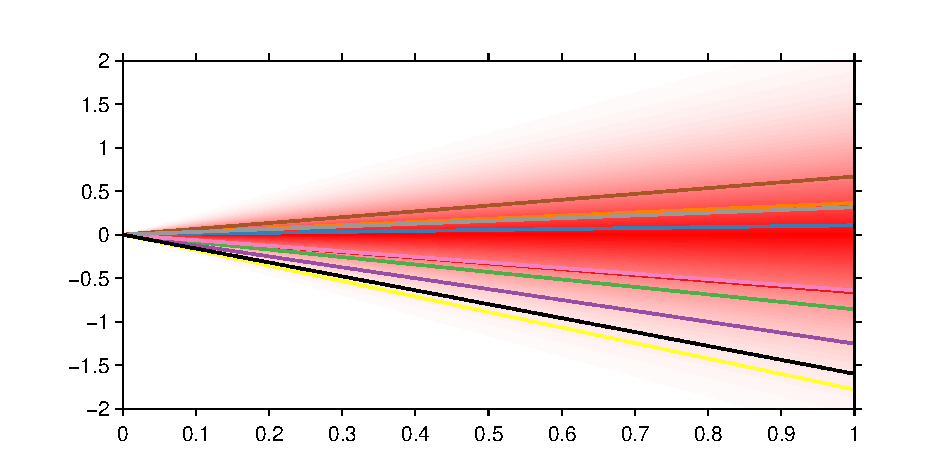
\includegraphics[width=0.3\columnwidth]{\introfigsdir/prior}
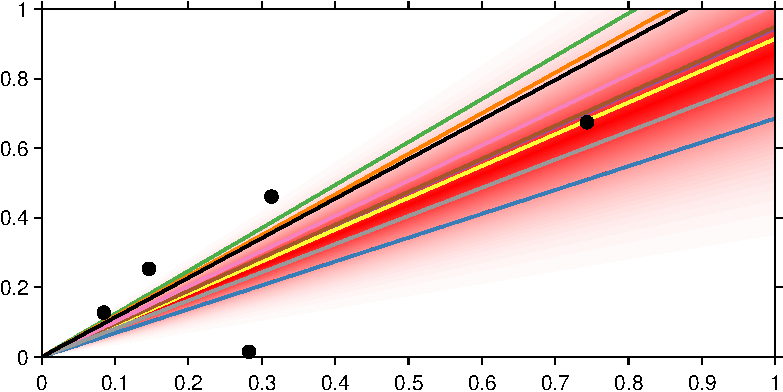
\includegraphics[width=0.3\columnwidth]{\introfigsdir/bayes_5}
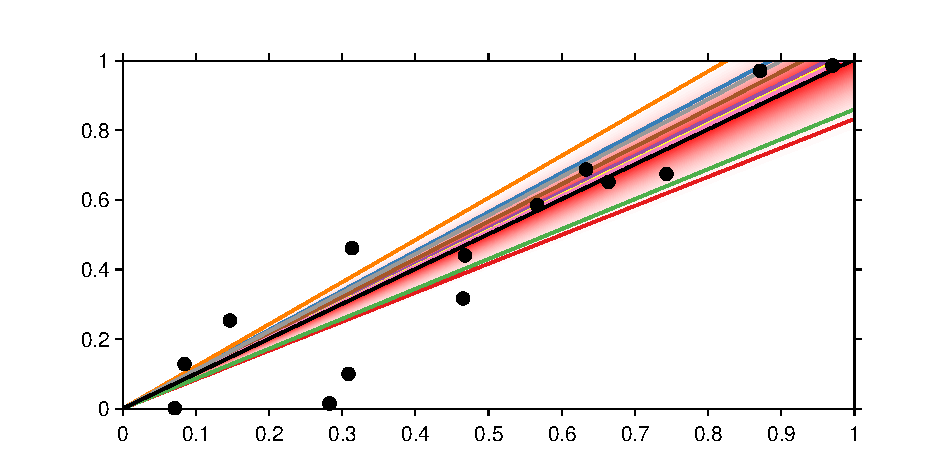
\includegraphics[width=0.3\columnwidth]{\introfigsdir/bayes_15}
\caption{
Bayesian linear regression.
\textit{Left}: Visualisation of prior distribution on gradient $m$.
Lines are random samples from the prior probability distribution, the red shading is a representation of the probability distribution.
\textit{Middle}: Visualiation of the posterior distribution for the gradient $m$ after 5 samples of data have been observed.
\textit{Right}: The posterior after 15 observations.
}
\label{fig:intro:lin_reg}
\end{figure}

We now rewrite the equations for the noisy linear relationship between $y$ and $x$ in an equivalent form
\[
  y_i &\sim \mathcal{N}(0, x_i^2 + \sigma_\varepsilon^2) \\
  \Cov(y_i, y_j) &= x_i x_j \quad \forall\,i\neq j
\]
\ie the prior distribution for $y$ has been assumed to be a multivariate Gaussian distribution
\[
  y \sim \Normal(0, K)
\]
where $K_{ij} = x_i x_j + \delta_{ij} \sigma_\varepsilon^2$ and $\delta_{ij}$ is the Kronecker delta.
Note that we can write this equation for the covariance as a function of pairs of inputs
\[
K_{ij} = k(x_i, x_j) = x_i x_j + \delta_{x_ix_j} \sigma_\varepsilon^2 \label{eq:intro:lin_noise_k}
\]
and this relationship holds for datasets of arbitrary finite size\footnotemark{}.
We now may reasonably ask whether or not we could define a probability distribution over $y$ when $x$ is infinite \eg when $x = \Reals$.
The answer to this question is yes.

\footnotetext{
We are implicitly assuming that the $x_i$ are disjoint.
This can be relaxed without any conceptual difficulty.
}

\begin{definition}[Gaussian process]
  A Gaussian process (\gp{}) is a collection of random variables, any finite subset of which have a joint Gaussian distribution.
\end{definition}

To specify a Gaussian process we must specify the mean and covariance of any finite subset of random variables which we achieve with a mean function $\mu : \mathcal{X} \to \Reals$ and a covariance function or kernel $k : \mathcal{X}^2 \to \Reals$ where $\mathcal{X}$ is the space inhabited by the inputs $x$ which can be written
\[
  y_i &\sim \mathcal{N}(\mu(x_i), k(x_i, x_i)) \\
  \Cov(y_i, y_j) &= k(x_i, x_j)
\]
or alternatively
\[
  (y_i : i = 1,\dots,n) \sim \Normal\bigg(\big(\mu(x_i) : i = 1,\dots,n\big), K\bigg)
\]
where $K_{ij} = k(x_i, x_j)$; note that $k$ must be such that $K$ is always positive (semi) definite to define a valid probability distribution.
Since these equations hold for any value of the inputs $x$ we can see that by writing $y_i = f(x_i)$ we have essentially specified a probability distribution over functions $f$.
We denote this distribution as
\[
  f \sim \gp(\mu,k).
\]

It is now reasonable to enquire as to the properties of this probability distribution over functions as we change $\mu$ and $k$.
The role of the mean function $\mu$ is particularly easy to characterise; it specifies the pointwise mean of this distribution over functions.
The covariance or kernel $k$ is more interesting.
Random samples from Gaussian processes with a zero mean function but different kernels are shown in figure~\ref{fig:intro:samples}; the randomly sampled functions display qualitatively different patterns of linearity, smoothness and periodicity.

\begin{figure}[ht]
\centering
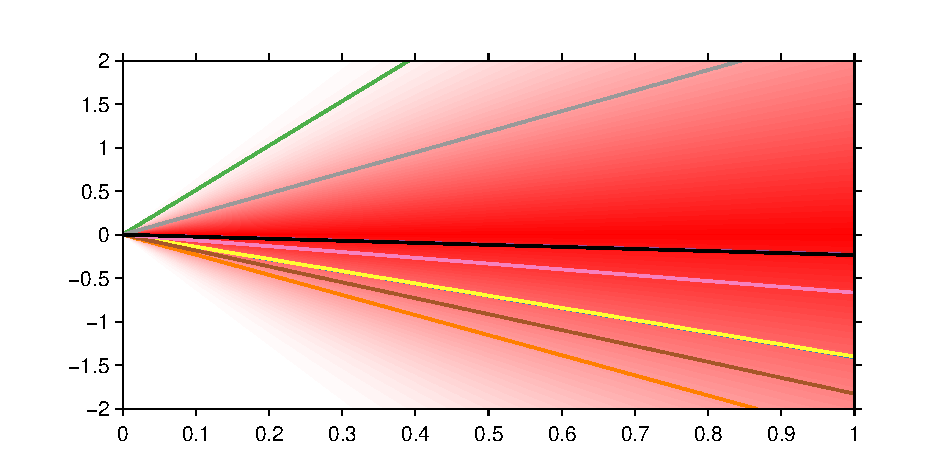
\includegraphics[width=0.3\columnwidth]{\introfigsdir/lin_prior}
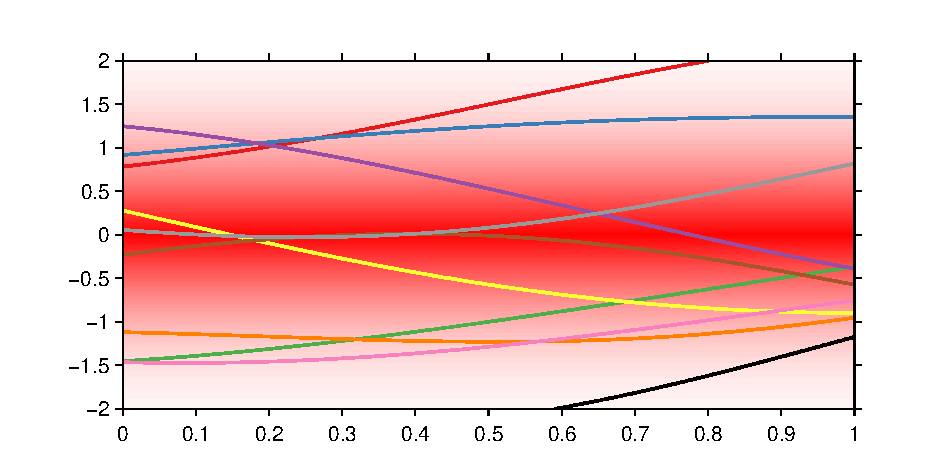
\includegraphics[width=0.3\columnwidth]{\introfigsdir/sq_exp_prior}
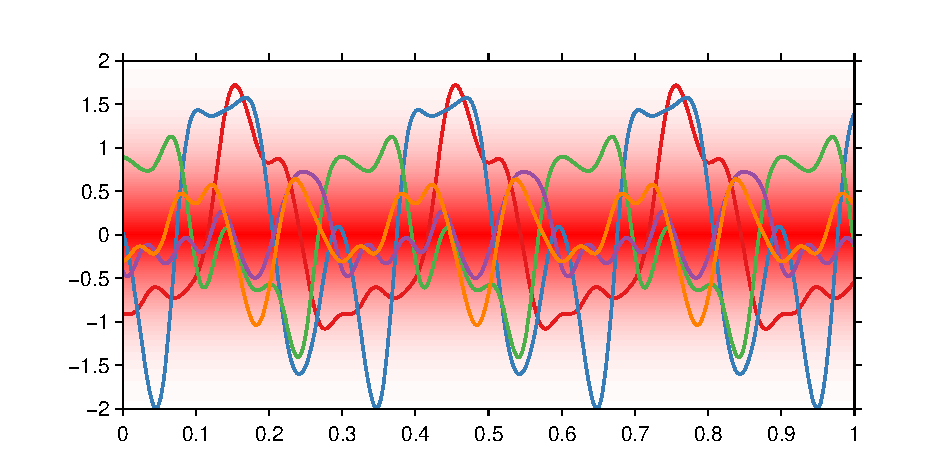
\includegraphics[width=0.3\columnwidth]{\introfigsdir/periodic_prior}
\caption{
Random samples from zero mean Gaussian processes with different covariance functions.
Lines are random samples from the Gaussian process distributions, the red shading is a representation of the pointwise probability distribution.
\textit{Left}: Linear functions.
\textit{Middle}: Smooth and slowly varying functions.
\textit{Right}: Smooth but exactly periodic functions.
}
\label{fig:intro:samples}
\end{figure}

The distribution over linear functions was constructed using a covariance of the form
\[
  k(x_i, x_j) = x_i x_j
\]
which is the same as that in equation~\eqref{eq:intro:lin_noise_k} with the noise variance equal to zero.

The distribution over smooth functions was constructed with a kernel of the form
\[
  k(x_i, x_j) = \exp(-\alpha|x_i - x_j|^2)
\]
where $\alpha$ is a constant.
When the distance between $x_i$ and $x_j$ is small, the covariance (and correlation) between $f(x_i)$ and $f(x_j)$ will be approximately equal to 1.
As a result, nearby values of the function will be similar to each other.
As the distance $|x_i - x_j|$ increases the correlation monotonically decreases to zero; the exact way in which the correlation decreases determines the characteristic smoothness one observes in figure~\ref{fig:intro:samples}.

Finally, the distribution over periodic functions was constructed using a covariance of the form
\[
  k(x_i, x_j) = \exp\left(-\frac{2\sin^2 (\pi(x_i - x_j)/p)}{\ell^2}\right)
\]
where $\ell$ and $p$ are constants.
Whenever $|x_i - x_j|$ is an integer multiple of $p$ the correlation is equal to 1 resulting in exact periodicity of the random functions.

In chapter~\ref{ch:construction} we demonstrate how to learn an appropriate kernel for a particular dataset by constructing new kernels from old.
In chapter~\ref{ch:description} we demonstrate that by carefully choosing which kernels we compose with each other we can always automatically produce natural language descriptions of the probability distributions they encode for.
In chapter~\ref{ch:gefcom} we demonstrate how these ideas were applied to a data mining competition and where this reveals scope for future work.

\outbpdocument{
\bibliographystyle{plainnat}
\bibliography{references.bib}
}



%
% A header that lets you compile a chapter by itself, or inside a larger document.
% Adapted from stackoverflow.com/questions/3655454/conditional-import-in-latex
%
%
%Use \inbpdocument and \outbpdocument in your individual files, in place of \begin{document} and \end{document}. In your main file, put in a \def \ismaindoc {} before including or importing anything.
%
% David Duvenaud
% June 2011
% 
% ======================================
%
%


\ifx\ismaindoc\undefined
	\newcommand{\inbpdocument}{
		\def \ismaindoc {}
		% Use this header if we are compiling by ourselves.
		\documentclass[a4paper,11pt,authoryear,index]{common/PhDThesisPSnPDF}
		
%\usepackage{draftwatermark}
%\SetWatermarkLightness{0.95}

% ******************************************************************************
% ****************************** Custom Margin *********************************

% Add `custommargin' in the document class options to use this section
% Set {innerside margin / outerside margin / topmargin / bottom margin}  and
% other page dimensions

\ifsetMargin
\else
    \RequirePackage[left=37mm,right=30mm,top=35mm,bottom=30mm]{geometry}
    \setFancyHdr % To apply fancy header after geometry package is loaded
\fi


%\chead{Unfinished draft}
%\cfoot{\texttt{Unfinished draft - compiled on \today{} at \currenttime}}

% *****************************************************************************
% ******************* Fonts (like different typewriter fonts etc.)*************

% Add `customfont' in the document class option to use this section

\ifsetFont
\else
    % Set your custom font here and use `customfont' in options. Leave empty to
    % load computer modern font (default LaTeX font).  

    \RequirePackage{libertine} 
\fi

% *****************************************************************************
% *************************** Bibliography  and References ********************

%\usepackage{cleveref} %Referencing without need to explicitly state fig /table

% Add `custombib' in the document class option to use this section
\ifsetBib % True, Bibliography option is chosen in class options
\else % If custom bibliography style chosen then load bibstyle here

   \RequirePackage[square, sort, numbers, authoryear]{natbib} % CustomBib

% If you would like to use biblatex for your reference management, as opposed to the default `natbibpackage` pass the option `custombib` in the document class. Comment out the previous line to make sure you don't load the natbib package. Uncomment the following lines and specify the location of references.bib file

% \RequirePackage[backend=biber, style=numeric-comp, citestyle=numeric, sorting=nty, natbib=true]{biblatex}
% \bibliography{References/references} %Location of references.bib only for biblatex

\fi


% changes the default name `Bibliography` -> `References'
\renewcommand{\bibname}{References}


% *****************************************************************************
% *************** Changing the Visual Style of Chapter Headings ***************
% Uncomment the section below. Requires titlesec package.

%\RequirePackage{titlesec}
%\newcommand{\PreContentTitleFormat}{\titleformat{\chapter}[display]{\scshape\Large}
%{\Large\filleft{\chaptertitlename} \Huge\thechapter}
%{1ex}{}
%[\vspace{1ex}\titlerule]}
%\newcommand{\ContentTitleFormat}{\titleformat{\chapter}[display]{\scshape\huge}
%{\Large\filleft{\chaptertitlename} \Huge\thechapter}{1ex}
%{\titlerule\vspace{1ex}\filright}
%[\vspace{1ex}\titlerule]}
%\newcommand{\PostContentTitleFormat}{\PreContentTitleFormat}
%\PreContentTitleFormat


% *****************************************************************************
% **************************** Custom Packages ********************************
% *****************************************************************************


% ************************* Algorithms and Pseudocode **************************

%\usepackage{algpseudocode} 


% ********************Captions and Hyperreferencing / URL **********************

% Captions: This makes captions of figures use a boldfaced small font. 
%\RequirePackage[small,bf]{caption}

\RequirePackage[labelsep=space,tableposition=top]{caption} 
%\renewcommand{\figurename}{Figure} %to support older versions of captions.sty
\captionsetup{labelsep = colon,belowskip=12pt,aboveskip=4pt}

% ************************ Formatting / Footnote *******************************

%\usepackage[perpage]{footmisc} %Range of footnote options 


% ****************************** Line Numbers **********************************

%\RequirePackage{lineno}
%\linenumbers

% ************************** Graphics and figures *****************************

%\usepackage{rotating}
%\usepackage{wrapfig}
%\usepackage{float}
\usepackage{subfig} %note: subfig must be included after the `caption` package. 


% ********************************* Table **************************************

%\usepackage{longtable}
%\usepackage{multicol}
%\usepackage{multirow}
%\usepackage{tabularx}


% ***************************** Math and SI Units ******************************

\usepackage{amsfonts}
\usepackage{amsmath}
\usepackage{amssymb}
%\usepackage{siunitx} % use this package module for SI units


% ******************************************************************************
% ************************* User Defined Commands ******************************
% ******************************************************************************

% *********** To change the name of Table of Contents / LOF and LOT ************

%\renewcommand{\contentsname}{My Table of Contents}
%\renewcommand{\listfigurename}{List of figures}
%\renewcommand{\listtablename}{List of tables}


% ********************** TOC depth and numbering depth *************************

\setcounter{secnumdepth}{2}
\setcounter{tocdepth}{2}

% ******************************* Nomenclature *********************************

% To change the name of the Nomenclature section, uncomment the following line

%\renewcommand{\nomname}{Symbols}


% ********************************* Appendix ***********************************

% The default value of both \appendixtocname and \appendixpagename is `Appendices'. These names can all be changed via: 

%\renewcommand{\appendixtocname}{List of appendices}
%\renewcommand{\appendixname}{Appndx}

		% All my custom preamble stuff.  Shouldn't overlap with anything in official-preamble




% Paths to figure and table directories.
\newcommand{\symmetryfigsdir}{figures/symmetries}
\newcommand{\topologyfiguresdir}{figures/topology}
\newcommand{\infinitefiguresdir}{figures/infinite}
\newcommand{\grammarfiguresdir}{figures/grammar}
\newcommand{\introfigsdir}{figures/intro}
\newcommand{\gplvmfiguresdir}{figures/gplvm}
\newcommand{\warpedfiguresdir}{figures/warped-mixtures}
\newcommand{\deeplimitsfiguresdir}{figures/deep-limits}
\newcommand{\quadraturefigsdir}{figures/quadrature}
\newcommand{\additivefigsdir}{figures/additive}
\newcommand{\decompfigsdir}{figures/decomp}
\newcommand{\examplefigsdir}{figures/worked-example}

\usepackage{bm}  % for warped mixtures - is this necessary?
\usepackage{booktabs}
\usepackage{tabularx}
\usepackage{multirow}
\usepackage{datetime}
\renewcommand{\tabularxcolumn}[1]{>{\arraybackslash}m{#1}}
\usepackage{relsize}
\usepackage{graphicx}
\usepackage{amsmath,amssymb,textcomp}
\usepackage{nicefrac}
\usepackage{amsthm}
\usepackage{tikz}
\usetikzlibrary{arrows}
\usetikzlibrary{calc}
\usepackage{nth}
\usepackage{rotating}
\usepackage{array}
\usepackage{fp}
\usepackage{cleveref}   % Note: this package sometimes causes the page counter to reset.
\crefname{equation}{equation}{equations}
\crefname{figure}{figure}{figures}
%\usepackage{common/sectsty}

% Controls capitalization of all headers
%\usepackage{stringstrings}
%\usepackage[explicit]{titlesec}
%\newcommand\SentenceCase[1]{%
%  \caselower[e]{#1}%
%  \capitalize[q]{\thestring}%
%}
%\titleformat{\section}
%  {\normalfont\Large\bfseries}{\thesection}{1em}{\SentenceCase{#1}\thestring}


%\titleformat{\section} % The normal, unstarred version
%    {\Large\bfseries}{}{2ex}
%    {\thesection. \MakeSentenceCase{#1}}

%\titleformat{name=\section,numberless} % The starred version; note the `numberless` key
%    {\Large\bfseries}{}{2ex}
%    {\MakeSentenceCase{#1}}

\usepackage[hyperpageref]{backref}
% Setup to show (pages 4 and 9) sort of thing in the bibliography - DD
%\def\foo{\hspace{\fill}\mbox{}\linebreak[0]\hspace*{\fill}}
%\def\foo{\parbox{3cm}{\hfill}
%\def\foo{\parbox{3cm}{\hfill}
%\newcommand\foo[1]{{\raggedleft{\hfill{\mbox{\hfill{#1}}}}}}
\newcommand{\comfyfill}[1]{% = Thorsten Donig's \signed
  \unskip\hspace*{0.1em plus 1fill}
  \nolinebreak[3]%
  \hspace*{\fill}\mbox{#1}
  \parfillskip0pt\par
}
\newcommand\foo[1]{{\comfyfill{\mbox{#1}}}}
%\newcommand\foo[1]{{\mbox{#1}}}
\renewcommand*{\backref}[1]{}
\renewcommand*{\backrefalt}[4]{%
\ifcase #1 %
%
\or
\foo{(page #2)}%
\else
\foo{(pages #2)}%
\fi
}

\usepackage{stringstrings}

%\newcommand{\headercase}{\
%\DeclareFieldFormat{titlecase}{\MakeSentenceCase{#1}}


%% For submission, make all render blank.
\input{common/commenting.tex}
%\renewcommand{\LATER}[1]{}
%\renewcommand{\fLATER}[1]{}
%\renewcommand{\TBD}[1]{}
%\renewcommand{\fTBD}[1]{}
%\renewcommand{\PROBLEM}[1]{}
%\renewcommand{\fPROBLEM}[1]{}
%\renewcommand{\NA}[1]{}


% HUMBLE WORDS: shown slightly smaller when in normal text
% Thanks to Christian Steinruecken!
\input{common/humble.tex}


% TODO: Clean up duplicates
\declareHumble{ANOVA}{ANOVA}
\declareHumble{ARD}{ARD}
\declareHumble{BIC}{BIC}
\declareHumble{BMC}{BMC}
\declareHumble{bq}{BQ}
\declareHumble{CRP}{CRP}
\declareHumble{dirpro}{DP}
\declareHumble{HDMR}{HDMR}
\declareHumble{GAM}{GAM}
\declareHumble{GEM}{GEM}
\declareHumble{GMM}{GMM}
\declareHumble{gplvm}{GP-LVM}
\declareHumble{gpml}{GPML}
\declareHumble{GPML}{GPML}
\declareHumble{gprn}{GPRN}
\declareHumble{gpt}{GP}
\declareHumble{gp}{GP}
\declareHumble{HKL}{HKL}
\declareHumble{HMC}{HMC}
\declareHumble{ibp}{IBP}
\declareHumble{iGMM}{iGMM}
\declareHumble{iwmm}{iWMM}
\declareHumble{kCP}{CP}
\declareHumble{kCW}{CW}
\declareHumble{kC}{C}
\declareHumble{KDE}{KDE}
\declareHumble{kLin}{Lin}
\declareHumble{KPCA}{KPCA}
\declareHumble{kPer}{Per}
\declareHumble{kPerGen}{ZMPer}
\declareHumble{kRQ}{RQ}
\declareHumble{kSE}{SE}
\declareHumble{kWN}{WN}
\declareHumble{Lin}{Lin}
\declareHumble{LBFGS}{L-BFGS}
\declareHumble{LIBSVM}{LIBSVM}
\declareHumble{MAP}{MAP}
\declareHumble{mcmc}{MCMC}
\declareHumble{MKL}{MKL}
\declareHumble{MLP}{MLP}
\declareHumble{MNIST}{MNIST}
\declareHumble{MSE}{MSE}
\declareHumble{OU}{OU}
\declareHumble{Per}{Per}
\declareHumble{RBF}{RBF}
\declareHumble{RMSE}{RMSE}
\declareHumble{RQ}{RQ}
\declareHumble{SBQ}{SBQ}
\declareHumble{seard}{SE-ARD}
\declareHumble{sefull}{SE-\textnormal{full}}
\declareHumble{SEGP}{SE-GP}
\declareHumble{SE}{SE}
\declareHumble{SNR}{SNR}
\declareHumble{SSANOVA}{SS-ANOVA}
\declareHumble{SVM}{SVM}
\declareHumble{UCI}{UCI}
\declareHumble{UMIST}{UMIST}
\declareHumble{vbgplvm}{VB GP-LVM}

\newcommand{\kSig}{\boldsymbol\sigma}

\def\subexpr{{\cal S}}
\def\baseker{{\cal B}}
\def\numWinners{k}

\def\ie{i.e.\ }
\def\eg{e.g.\ }
\def\etc{etc.\ }
\let\oldemptyset\emptyset
%\let\emptyset 0




% Unify notation between neural-net land and GP-land.
\newcommand{\hphi}{h}
\newcommand{\hPhi}{\vh}
\newcommand{\walpha}{w}
\newcommand{\wboldalpha}{\bw}
\newcommand{\wcapalpha}{\vW}
\newcommand{\lengthscale}{w}

\newcommand{\layerindex}{\ell}



\newcommand{\gpdrawbox}[1]{
\setlength\fboxsep{0pt}
\hspace{-0.15in} 
\fbox{
\includegraphics[width=0.464\columnwidth]{\deeplimitsfiguresdir/deep_draws/deep_gp_sample_layer_#1}
}}



\newcommand{\procedurename}{ABCD}
\newcommand{\genText}[1]{{\sf #1}}



\newcommand{\asdf}{$^{\textnormal{th}}$}

\newcommand{\binarysum}{\sum_{\bf{x} \in \{0,1\}^D}}
\newcommand{\expect}{\mathbb{E}}
\newcommand{\expectargs}[2]{\mathbb{E}_{#1} \left[ {#2} \right]}
\newcommand{\var}{\mathbb{V}}
\newcommand{\varianceargs}[2]{\mathbb{V}_{#1} \left[ {#2} \right]}
\newcommand{\cov}{\operatorname{cov}}
\newcommand{\Cov}{\operatorname{Cov}}
\newcommand{\covargs}[2]{\Cov \left[ {#1}, {#2} \right]}
\newcommand{\variance}{\mathbb{V}}
\newcommand{\vecop}[1]{\operatorname{vec} \left( {#1} \right)}

\newcommand{\covarianceargs}[2]{\Cov_{#1} \left[ {#2} \right]}
\newcommand{\colvec}[2]{\left[ \begin{array}{c} {#1} \\ {#2} \end{array} \right]}
\newcommand{\tbtmat}[4]{\left[ \begin{array}{cc} {#1} & {#2} \\ {#3} & {#4} \end{array} \right]}

\newcommand{\acro}[1]{{\humble{#1}}}
%\newcommand{\vect}[1]{\boldsymbol{#1}}
\newcommand{\vect}[1]{{\bf{#1}}}
\newcommand{\mat}[1]{\mathbf{#1}}
\newcommand{\pderiv}[2]{\frac{\partial #1}{\partial #2}}
\newcommand{\npderiv}[2]{\nicefrac{\partial #1}{\partial #2}}

\newcommand{\pha}{^{\phantom{:}}}

\newcommand{\argmin}{\operatornamewithlimits{argmin}}
\newcommand{\argmax}{\operatornamewithlimits{argmax}}

% The following designed for probabilities with long arguments

\newcommand{\Prob}[2]{P\!\left(\,#1\;\middle\vert\;#2\,\right)}
\newcommand{\ProbF}[3]{P\!\left(\,#1\!=\!#2\;\middle\vert\;#3\,\right)}
\newcommand{\p}[2]{p\!\left(#1\middle\vert#2\right)}
\newcommand{\po}[1]{p\!\left(#1\right)}
\newcommand{\pF}[3]{p\!\left(\,#1\!=\!#2\;\middle\vert\;#3\,\right)} 
\newcommand{\mean}[2]{{m}\!\left(#1\middle\vert#2\right)}



\newcommand{\valpha}{\boldsymbol{\alpha}}
\newcommand{\va}{\vect{a}}
\newcommand{\vA}{\vect{A}}
\newcommand{\vB}{\mat{B}}
\newcommand{\vb}{\vect{b}}
\newcommand{\vC}{\mat{C}}
\newcommand{\vc}{\vect{c}}
\newcommand{\vecf}{\boldsymbol{f}}
\newcommand{\vell}{\vect{\ell}}
\newcommand{\vepsilon}{\boldsymbol{\epsilon}}
\newcommand{\veps}{\boldsymbol{\epsilon}}
\newcommand{\ve}{\boldsymbol{\epsilon}}
\newcommand{\vf}{\vecf}
\newcommand{\vg}{\vect{g}}
\newcommand{\vh}{\vect{h}}
\newcommand{\vI}{\mat{I}}
\newcommand{\vK}{\mat{K}}
\newcommand{\vk}{\vect{k}}
\newcommand{\vL}{\mat{L}}
\newcommand{\vl}{\vect{l}}
\newcommand{\vmu}{{\boldsymbol{\mu}}}
\newcommand{\vone}{\vect{1}}
\newcommand{\vphi}{{\boldsymbol{\phi}}}
\newcommand{\vpi}{{\boldsymbol{\pi}}}
\newcommand{\vq}{\vect{q}}
\newcommand{\vR}{\mat{R}}
\newcommand{\vr}{\vect{r}}
\newcommand{\vsigma}{{\boldsymbol{\sigma}}}
\newcommand{\vSigma}{\mat{\Sigma}}
\newcommand{\vS}{\mat{S}}
\newcommand{\vs}{\vect{s}}
\newcommand{\vtheta}{{\boldsymbol{\theta}}}
\newcommand{\vu}{\vect{u}}
\newcommand{\vV}{\mat{V}}
\newcommand{\vW}{\mat{W}}
\newcommand{\vw}{\vect{w}}
\newcommand{\vX}{\mat{X}}
\newcommand{\vx}{\vect{x}}
\newcommand{\vY}{\mat{Y}}
\newcommand{\vy}{\vect{y}}
\newcommand{\vzero}{\vect{0}}
\newcommand{\vZ}{\mat{Z}}
\newcommand{\vz}{\vect{z}}


% deep gp notation
\newcommand{\netweights}{w}
\newcommand{\vnetweights}{\vw}
\newcommand{\mnetweights}{\vW}
\newcommand{\outweights}{\v}
\newcommand{\voutweights}{\vv}
\newcommand{\moutweights}{\vV}

\newcommand{\unitparams}{\v}
\newcommand{\vunitparams}{\vv}
\newcommand{\munitparams}{\vV}


\newcommand{\He}{\mathcal{H}}
\newcommand{\normx}[2]{\left\|#1\right\|_{#2}}
\newcommand{\Hnorm}[1]{\normx{#1}{\He}}
\newcommand{\mmd}{{\rm MMD}}


\newcommand{\mf}{\bar{\vf}}

%\newcommand{\mf}{\mu} %{\bar{\ell}}
\newcommand{\lf}{f} % Likelihood function
\newcommand{\st}{_\star}

% from simpler log-bq writeup
\newcommand{\lftwo}{{\log \ell}}
\newcommand{\mftwo}{{\bar \ell}}
\newcommand{\loggp}{{\log\acro{GP}}}%| \bX, \vy )}}
\newcommand{\loggpdist}{{\acro{GP}(\lftwo)}}%| \vX, \vy )}}


\newcommand{\inv}{^{{\mathsmaller{-1}}}}
\newcommand{\tohalf}{^{{\mathsmaller{\nicefrac{1}{2}}}}}

\newcommand{\Normal}{\mathcal{N}}
\newcommand{\N}[3]{\mathcal{N}\!\left(#1 \middle| #2,#3\right)}
\newcommand{\Nt}[2]{\mathcal{N}\!\left(#1,#2\right)}
\newcommand{\NT}[2]{\mathcal{N}\!\left(#1,#2\right)}
\newcommand{\GPdist}[3]{\mathcal{GP}\!\left(#1 \, \middle| \, #2, #3 \right)}
\newcommand{\GPdisttwo}[2]{\mathcal{GP}\!\left(\, #1, #2 \right)}
\newcommand{\bN}[3]{\mathcal{N}\big(#1 \middle| #2,#3\big)}
\newcommand{\boldN}[3]{\text{\textbf{\mathcal{N}}}\big(#1;#2,#3\big)}
\newcommand{\ones}[1]{\mat{1}_{#1}}
\newcommand{\eye}[1]{\mat{E}_{#1}}
\newcommand{\tra}{^{\mathsf{T}}}
%\newcommand{\tra}{^{\top}}
%\mathsf{T}
\newcommand{\trace}{\operatorname{tr}}
\newcommand{\shift}{\operatorname{shift}}
\renewcommand{\mod}{\operatorname{mod}}
\newcommand{\deq}{:=}
\newcommand{\oneofk}{\operatorname{one-of-k}}
%\newcommand{\degree}{^\circ}

\newcommand{\GPt}[2]{\mathcal{GP}\!\left(#1,#2\right)}
%\newcommand{\GPt}[2]{\gp\!\left(#1,#2\right)}

\DeclareMathOperator{\tr}{tr}
\DeclareMathOperator{\chol}{chol}
\DeclareMathOperator{\diag}{diag}

\newenvironment{narrow}[2]{%
  \begin{list}{}{%
  \setlength{\topsep}{0pt}%
  \setlength{\leftmargin}{#1}%
  \setlength{\rightmargin}{#2}%
  \setlength{\listparindent}{\parindent}%
  \setlength{\itemindent}{\parindent}%
  \setlength{\parsep}{\parskip}}%
\item[]}{\end{list}}



\newcommand{\dist}{\ \sim\ }
\def\given{\,|\,}

% Table stuff
\newcolumntype{C}[1]{>{\centering\let\newline\\\arraybackslash\hspace{0pt}}m{#1}}
\newcolumntype{L}[1]{>{\raggedright\let\newline\\\arraybackslash\hspace{0pt}}m{#1}}
\newcolumntype{R}[1]{>{\raggedleft\let\newline\\\arraybackslash\hspace{0pt}}m{#1}}

\newcommand{\defeq}{\mathrel{:\mkern-0.25mu=}}

\def\ie{i.e.\ }
\def\eg{e.g.\ }
\def\iid{i.i.d.\ }
%\def\simiid{\sim_{\mbox{\tiny iid}}}
\def\simiid{\overset{\mbox{\tiny iid}}{\sim}}
\def\simind{\overset{\mbox{\tiny \textnormal{ind}}}{\sim}}
\def\eqdist{\stackrel{\mbox{\tiny d}}{=}}
%\newcommand{\distas}[1]{\mathbin{\overset{#1}{\kern \z@ \sim}}}
%TODO: fix this - it worked outside the thesis!
\newcommand{\distas}[1]{\mathbin{\overset{#1}{\sim}}}

\def\Reals{\mathbb{R}}

\def\Uniform{\mbox{\rm Uniform}}
\def\Bernoulli{\mbox{\rm Bernoulli}}
\def\GP{\mathcal{GP}}
\def\GPLVM{\mathcal{GP-LVM}}




% Kernel stuff

\def\iva{\vect{\inputVar}}
\def\ivaone{\inputVar}
\def\inputVar{x}
\def\InputVar{X}
\def\InputSpace{\mathcal{X}}
\def\outputVar{y}
\def\OutputSpace{\mathcal{Y}}
\def\function{f}
\def\kernel{k}
\def\KernelMatrix{K}
\def\SumKernel{\sum}
\def\ProductKernel{\prod}
\def\expression{e}
\def\feat{\vh}

\newcommand{\kerntimes}{ \! \times \!}
\newcommand{\kernplus}{ \, + \,}


% Proof stuff
\theoremstyle{plain}
\newtheorem{theorem}{Theorem}[section]
\newtheorem{lemma}[theorem]{Lemma}
\newtheorem{prop}[theorem]{Proposition}
\newtheorem{proposition}{Proposition}
\newtheorem*{cor}{Corollary}

% For infinite bq
\newcommand{\iv}{\theta}
\newcommand{\viv}{\vtheta}

% For intro chapter
\newcommand{\funcval}{\vf(\vX)}
\newcommand{\testpoint}{{\vx^\star}}

\newcommand{\underwrite}[2]{{\underbrace{#1}_{\textnormal{#2}}}}



% For kernel figures
\newcommand{\fhbig}{2cm}%
\newcommand{\fwbig}{3cm}%
\newcommand{\kernpic}[1]{\includegraphics[height=\fhbig,width=\fwbig]{\grammarfiguresdir/structure_examples/#1}}%
\newcommand{\kernpicr}[1]{\rotatebox{90}{\includegraphics[height=\fwbig,width=\fhbig]{\grammarfiguresdir/structure_examples/#1}}}%
\newcommand{\addkernpic}[1]{{\includegraphics[height=\fhbig,width=\fwbig]{\grammarfiguresdir/additive_multi_d/#1}}}%
\newcommand{\largeplus}{\tabbox{{\Large+}}}%
\newcommand{\largeeq}{\tabbox{{\Large=}}}%
\newcommand{\largetimes}{\tabbox{{\Large$\times$}}}%
\newcommand{\fixedx}{$x$ (with $x' = 1$)}%

% for warped mixtures
\newcommand{\CLAS}{\vz}  %cluster assignments
\newcommand{\CLASi}{z} % individual cluster assignments


		% ************************ Thesis Information & Meta-data **********************

%% The title of the thesis
\title{Automating statistical modelling}

%\texorpdfstring is used for PDF metadata. Usage:
%\texorpdfstring{LaTeX_Version}{PDF Version (non-latex)} eg.,
%\texorpdfstring{$sigma$}{sigma}

%% The full name of the author
\author{James Robert Lloyd}

%% Department (eg. Department of Engineering, Maths, Physics)
%\dept{Department of Engineering}

%% University and Crest
\university{University of Cambridge}
\crest{
\includegraphics[width=0.25\textwidth]{misc/University_Crest}}

%% You can redefine the submission text:
% Default as per the University guidelines: This dissertation is submitted for
% the degree of Doctor of Philosophy
%\renewcommand{\submissiontext}{change the default text here if needed}

%% Full title of the Degree 
\degree{Doctor of Philosophy}
 
%% College affiliation (optional)
\college{Trinity College}

%% Submission date
\degreedate{December 2014} 

%% Meta information
\subject{Machine Learning}
\keywords{{LaTeX} {PhD Thesis} {Engineering} {University of Cambridge} {Machine Learning} {Gaussian processes} {Time Series} {Model checking} {Model criticism} {Aldous--Hoover} {Networks}}



		\begin{document}
	}	
	\newcommand{\outbpdocument}[1]{
		% Fake chapters so references aren't broken
		\label{ch:intro}                
		\label{ch:dummy}
		\label{ch:discussion}
		%\bibliographystyle{common/CUEDthesis}
		\bibliographystyle{plainnat}
		\bibliography{references.bib}
		\end{document}
	}	
\else
	%If we're inside another document, no need to re-start the document.
	\ifx\inbpdocument\undefined
		\newcommand{\inbpdocument}{}
		\newcommand{\outbpdocument}[1]{}
	\fi
\fi

\inbpdocument

\chapter{Statistical models for networks}
\label{ch:networks}

In much of the machine learning literature, data can naturally be viewed as a sequence or a list.
Of course, there are many other types and structures of data, such as those which are most naturally represented as a network.
In this chapter we make the distinction between these types of data precise by symmetry arguments and invoke a theorem due to Aldous and Hoover to demonstrate appropriate forms of statistical model for these data types.
In particular, we propose a nonparametric model of networks as a literal interpretation of this theorem.
In chapter~\ref{ch:arrays} we extend these results to yet more data structures.

This chapter is based on joint work with Peter Orbanz, Zoubin Ghahramani and Daniel Roy \citep{Lloyd2012-sb}.

\section{Introduction}

Relational data records relations between entities.
Such data arises in a variety of contexts, including graph-valued data \citep[e.g.][]{Airoldi2008-fr,Hoff2002-vy}, micro-array data, tensor data \citep[e.g.][]{Xu2012-ub} and collaborative filtering \citep[e.g.][]{Salakhutdinov2008-tp}.
Pairwise relations can be summarized in a 2-dimensional array (often also called a matrix);
more generally, relations between $d$-tuples are recorded as $d$-dimensional arrays.
We consider probabilistic models of infinite 2-arrays $\{\darray_{ij} : i,j\in\Nats\}$, where entries $\darray_{ij}$ take values in a space $\dataspace$. 
Each entry $\darray_{ij}$ describes the relation between objects $i$ and $j$. Finite
samples---relational measurements for $n$ objects---are $n\times n$-arrays. As the sample size increases, the data aggregates into
a larger and larger array. 
Graph-valued data, for example, corresponds to the case $\dataspace=\lbrace{0,1}\rbrace$.
In collaborative filtering problems, the set of objects is subdivided into two disjoint sets, \eg users and items.
This corresponds to a bipartite graph if the relations are additionally binary.

Latent variable models for relational data explain observations by means of an underlying structure
or summary,
such as a low-rank approximation to an observed matrix or an embedding into a Euclidean space.
This structure is formalized as a latent (unobserved) variable.
Examples of such models include probabilistic matrix factorization (PMF) \citep{Salakhutdinov2008-tp}, the eigenmodel of 
\citet{Hoff2007-ja}, the mixed-membership stochastic blockmodel (MMSB) \citep{Airoldi2008-fr}
and the Gaussian process latent variable model (GPLVM) \citep[e.g.][]{Lawrence2009-za}.

\citet{Hoff2007-ja} first noted that latent variable models of relational data can be justified by an exchangeability or symmetry argument.
Building on this connection, we consider nonparametric models for graphs and arrays.
Results of
Aldous \cite{Aldous1981-lg}, Hoover \cite{Hoover1979-br} and Kallenberg \cite{Kallenberg1992-gb} show
that random arrays which satisfy an exchangeability property can be represented in terms of a random
function. These representations have been further developed in discrete analysis for the
special case of graphs \citep{Lovasz2006-hc}; this case is illustrated in Fig.~\ref{fig:W:graph}.
The results can be regarded as a generalization of de Finetti's theorem to array-valued data.
Their implication for probabilistic modelling is that
\emph{we can specify a probability distribution for an exchangeable random array by specifying a probability distribution on (measurable) functions}.
%The prior is in general a distribution on the space of all functions which can arise in the representation result, and the dimension of this space is infinite.
% A prior must hence be nonparametric to have reasonably large support; a parametric prior concentrates on a finite-dimensional subset.
In this chapter, we model this function explicitly using a nonparametric distribution over functions.

\begin{figure}
 \begin{center}
    \begin{tikzpicture}[>=stealth,scale=2.4]%,transform canvas={xshift=-3cm,yshift=1cm}]
  \begin{scope}[yshift=0.5cm]
  \begin{scope}
    %\path[use as bounding box] (-0.5,0.5) rectangle (2.8,-1.5);
    \draw (0,0) --(0,-1) --(1,-1) --(1,0) --(0,0);
    %\draw (0,0)--(1,-1);
    \node[font=\scriptsize] at (0,0.1) {$0$};
    \node[font=\scriptsize] at (-0.1,0) {$0$};
    \node[font=\scriptsize] at (1,-1.1) {$1$};
    \node[font=\scriptsize] at (1.1,-1) {$1$};
    \draw [dashed] (0.2,0.1) -- (0.2,-1.1); \node at (0.2,0.2) {$U_1$};
    \draw [dashed] (-0.1,-0.2) -- (1.1,-0.2); \node at (-0.25,-0.2) {$U_1$};
    \draw [dashed] (0.65,0.1) -- (0.65,-1.1); \node at (0.65,0.2) {$U_2$};
    \draw [dashed] (-0.1,-0.65) -- (1.1,-0.65); \node at (-0.25,-0.65) {$U_2$};
    \node[circle,fill,scale=0.4,color=red] at (0.65,-0.2) {};
  \end{scope}
  \begin{scope}[xshift=2cm]
    \draw (0,0)--(0,-1);
    \draw (-0.05,0)--(0.05,0); \node at (0.15,0) {$0$};
    \draw (-0.05,-1)--(0.05,-1); \node at (0.15,-1) {$1$};
    \node[circle,fill,scale=0.4,color=red] at (0,-0.21) {};
    \node[font=\scriptsize] at (0.38,-0.23) {$\mbox{Pr}\lbrace X_{ij}=1\rbrace$};
  \end{scope}
  \begin{scope}
  \draw[->] (0.7,-0.25) .. controls (1.3,-0.5) and (1.5,-0.5) .. (1.95,-0.26);
  \draw (1.4,-0.45) node [fill=white] {$\Theta$};
  \end{scope}
  \end{scope}
  \begin{scope}[xshift=3.4cm]
    \node [mybox] (box){
    
\includegraphics[width=2.9cm]{\networksfigsdir/uniform_attachment_graphon.pdf}
  };
  \end{scope}  
  \begin{scope}[xshift=4.8cm]
    \node [mybox] (box){
    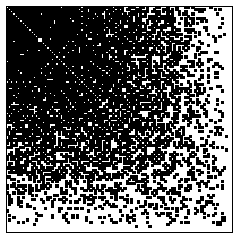
\includegraphics[width=2.8cm]{\networksfigsdir/uniform_attachment_empirical.pdf}
  };
  \end{scope}
\end{tikzpicture}

  \end{center}
 \caption{\emph{Left:} Any exchangeable random graph with vertex set $\Nats$ and edges ${E=(\darray_{ij})_{i,j\in\Nats}}$ can be represented
   by a random function ${\Theta:[0,1]^2\rightarrow[0,1]}$. Given $\AHfunction$, a graph can be sampled by generating a uniform random 
   variable $\AHvar_i$ for each vertex $i$, and sampling edges as ${\darray_{ij}\sim\Bernoulli(\AHfunction(\AHvar_i,\AHvar_j))}$.
   \emph{Middle:} A heat map of an example function $\AHfunction$.
   \emph{Right:} A ${100\times 100}$ symmetric adjacency matrix sampled from $\AHfunction$.
   Only unordered index pairs $\darray_{ij}$ are sampled in the symmetric case. Rows and columns are ordered
   by increasing value of $\AHvar_i$, rather than $i$.}
 \label{fig:W:graph}
\end{figure}


\section{Background: Exchangeable sequences and arrays}
\label{sec:background}

\subsection{Reminder: de Finetti's theorem}

Repeating from the main introduction to this thesis, suppose one receives a sequence of data $(X_1, X_2, \dots)$ and we wish to specify our beliefs about this data with a probability distribution.
An often reasonable prior assumption is that we do not believe the order of the data contains any information, or rather that any probability distribution encoding our beliefs about this data should be invariant to reorderings of the data.
That is, we may often believe that our data is an exchangeable sequence:
\[
  \label{eq:networks:exch}
  (X_1, X_2, \dots) \eqdist (X_{p(1)}, X_{p(2)}, \dots) \qquad \forall\, p\in\SGinf
\]
where $\eqdist$ denotes equality in distribution, and $\SGinf$ is the set of all permutations of $\Nats$ which permute at most a finite number of elements.

de Finetti's theorem \citep[e.g.][]{Kallenberg2002-il} characterises all probability distributions of sequences with this property;  $(X_i)_{i\in\Nats}$ is an exchangeable sequence if and only if there exists a random probability measure $\AHfunction$ such that $\darray_1,\darray_2,\ldots\simiid\AHfunction$.
In other words, observations are conditionally \iid given some random $\AHfunction$.
For the purposes of probabilistic modelling, this implies that our beliefs about exchangeable sequences of data can be expressed in the form of a distribution over probability measures.

\subsection{de Finetti-type representations for exchangeable arrays}

To specify probabilistic models for graph- or array-valued data, it would be helpful to have a suitable counterpart to de Finetti's theorem applicable when the infinite random sequences in \eqref{eq:networks:exch} are substituted by infinite random arrays $\darray=(\darray_{ij})_{i,j\in\Nats}$.
For such data, the invariance assumption \eqref{eq:networks:exch} is typically too restrictive: In the graph case $\darray_{ij}\in\lbrace 0,1\rbrace$, for example, the probability of $\darray$ would then depend only on the proportion of present edges in the graph, but not on the graph structure.
Instead, we define exchangeability of random 2-arrays in terms of the \emph{simultaneous} application of a permutation to rows and columns.
More precisely:
\begin{definition}
  An array $\darray=(\darray_{ij})_{i,j\in\Nats}$ is called a \emph{jointly exchangeable array} if 
  \begin{equation}
    \label{eq:jointly:ex}
    (\darray_{ij})\eqdist(\darray_{p(i)p(j)}) \qquad\text{ for every }pi\in\SGinf\;.
  \end{equation}
\end{definition}

The assumption of exchangeability stated in~\eqref{eq:networks:exch} states that the order of the data does not matter.
In contrast, array exchangeability is a statement of indifference to any ordering of the entities or objects that the data measures relations between.
In fact, exchangeable sequences can be viewed in this way too, the difference is that data is measured at individual entities or objects rather than at pairs.

Since this form of exchangeability weakens the hypothesis \eqref{eq:networks:exch} by demanding invariance only under a subset of all permutations of $\Nats^2$---those of the form $(i,j)\mapsto(p(i),p(j))$---we can no longer expect de Finetti's theorem to hold.
The relevant generalisation of the de Finetti theorem to this case is the following:
\begin{thm}[Aldous, Hoover]
  \label{theorem:ah}
  A random array $(\darray_{ij})$ is jointly exchangeable if and only if there is a random (measurable) function ${F:[0,1]^3\rightarrow\dataspace}$ such that the following holds: If $(\AHvar_i)_{i\in\Nats}$ and $(\AHvar_{\{ij\}})_{ij\in\Nats}$ are \iid sequences of ~$\Uniform[0,1]$ random variables, then
  \begin{equation}
    \label{eq:ah}
    (\darray_{ij})\eqdist (F(\AHvar_i,\AHvar_j,\AHvar_{\{ij\}})) \qquad\text{ for all }i,j\in\Nats\;.
  \end{equation}
\end{thm}

\begin{rem}%\fTBD{To be reviewed. I have made reference to simplicity}
\label{rem:U_ij}
Note that the symmetry of $(U_{\{ij\}})$ is not restrictive, in the sense that a representation where \eg $U_{ij}$ and $U_{ji}$ are \iid is trivially jointly exchangeable and thus can be given a representation of the above form.
%\NA{In section \ref{sec:simple} we describe a representation result which does not involve $(U_{ij})$ and thus the symmetry does not place a restriction on potential models of $\darray$.}\fTBD{DR: Need to think about this.}
\end{rem}
%\begin{rem}[symmetric arrays]\label{remsym}
%When modeling a symmetric array $X$, one can reduce the index set from ordered pairs $(i,j)$ to unordered pairs $\{i,j\}$.  
%In this case, $(X_{\{i,j\}}) \eqdist (F(U_i,U_j,U_{\{i,j\}}))$ where $F(\cdot,\cdot,d)$ is symmetric for every fixed value $d$.
%\end{rem}
\begin{rem}[separately exchangeable arrays]\label{remsep}
We say that an array $(X_{ij})$ is \emph{separately exchangeable} when $(X_{ij}) \eqdist (X_{p(i)p'(j)})$ for every pair $p,p' \in \SGinf$ of permutations. 
Such symmetry would be appropriate when modelling, e.g., a collaborative filtering task where the order of users and items are simultaneously irrelevant.
A separately exchangeable array can be seen to correspond with an off-diagonal subarray of a jointly exchangeable array, and thus can be shown to have the representation $(X_{ij}) \eqdist (F(U_i,V_j,W_{ij}))$, where $(U_i)$, $(V_j)$ and $(W_{ij})_{i,j\in\Nats}$ are \iid $\Uniform[0,1]$ random variables.
\end{rem}

\subsection{Random graphs}

The graph-valued data case $\dataspace=\lbrace{0,1}\rbrace$ is of particular interest. Here, the array $\darray$, interpreted as 
an adjacency matrix, specifies a random simple graph with vertex set $\Nats$. If $\darray$ is symmetric, the graph is undirected. We call a 
random graph exchangeable if $\darray$ satisfies \eqref{eq:jointly:ex}, \ie if its distribution is invariant under permutation of vertices.

For graphs, the representation \eqref{eq:ah} simplifies further:
For any exchangeable random graph, there is a random
function ${\AHfunction:[0,1]^2\rightarrow[0,1]}$ such that
\begin{equation}
  \label{eq:ah:graphon:case}
  %(\darray_{ij})\eqdist 
  F(\AHvar_i,\AHvar_j,\AHvar_{ij}):=\mathbb{I}\lbrace \AHvar_{ij} < \AHfunction(\AHvar_i,\AHvar_j)\rbrace\;.
\end{equation}
Each variable $\AHvar_i$ is associated with a vertex, each variable $\AHvar_{ij}$ with an edge. 
The representation \eqref{eq:ah:graphon:case} is equivalent to the sampling scheme
\begin{equation}
  \label{eq:W:graph}
  \AHvar_1,\AHvar_2,\dots\simiid\Uniform[0,1]\qquad\text{and}\qquad X_{i,j}\sim\Bernoulli(\AHfunction(\AHvar_i,\AHvar_j))\;,
\end{equation}
which is illustrated in Fig.~\ref{fig:W:graph}. If the graph is undirected, edges are sampled only for unordered index pairs as $\AHvar_{\lbrace ij\rbrace}$,
and it is sufficient to consider symmetric functions $\AHfunction$.

Recent work in discrete analysis shows that any measurable function $[0,1]^2\rightarrow[0,1]$ can be regarded as a (suitably defined) limit of adjacency matrices of graphs of increasing size \citep{Lovasz2006-hc}---intuitively speaking, 
as the number of rows and columns increases, the
matrix in Fig.~\ref{fig:W:graph} (right) converges to the heat map in Fig.~\ref{fig:W:graph} (middle).
The figure also illustrates that convergence, and hence the parametrisation of the random graph distribution
by $\AHfunction$, are only unique up to a reordering of rows and columns.

In particular, if we fix an instance ${\AHfunction=\theta_0}$ and generate a random graph according to \eqref{eq:W:graph},
we asymptotically recover the function $\theta_0$. This can be regarded as analogous to the law of large
numbers, guaranteeing that a distribution can asymptotically be recovered from a sample.

\subsection{The general case: $d$-arrays}

Theorem \ref{theorem:ah} can in fact be stated in a more general setting than matrices, namely for random $d$-arrays, which are collections
of random variables of the form ${\{\darray_{i_1\dots i_d} i_1,\dots,i_d\in\Nats\}}$. Thus, a sequence is a $1$-array, a matrix a $2$-array. A $d$-array 
can be interpreted as an encoding of a relation between $d$-tuples.
In this general case, Theorem \ref{theorem:ah} still holds, but the random function $F$ in \eqref{eq:ah} is in general more complex:
In addition to the collections $\AHvar_{\lbrace i\rbrace}$ and $\AHvar_{\lbrace ij\rbrace}$ of uniform variables, the representation requires an additional
collection $\AHvar_{\lbrace i_j\rbrace_{j\in I}}$ for any non-empty subset $I$ of the set $\lbrace 1,\ldots,d\rbrace$; \eg
$\AHvar_{i_1 i_3 i_4}$ for $d\geq 4$ and ${I=\lbrace 1,3,4\rbrace}$. The representation \eqref{eq:ah} is then substituted by
\begin{equation}
  F:[0,1]^{2^d-1}\longrightarrow\dataspace\qquad\text{and}\qquad \darray_{i_1,\dots,i_d}=F(\AHvar_{I_1},\dots,\AHvar_{I_{(2^d-1)}})\;.
\end{equation}
For $d=1$, we recover de Finetti's theorem. In particular, if $\dataspace=\mathbb{R}$, $F$ is given by the inverse cumulative distribution function
of the random measure guaranteed by de Finetti's theorem.
For a discussion of convergence properties of general arrays similar to those sketched above for random graphs, see  \citep{Aldous2010-iw}.

Since we do not explicitly consider the case $d>2$ in our experiments in this chapter, we restrict 
our presentation throughout to the matrix-valued case for simplicity.
We note, however, that the model and inference algorithms described in the following are applicable to general array-valued data.
In chapter \ref{ch:arrays} we extend these representation results to arbitrary collections of arrays of arbitrary size.

\section{A nonparametric model of exchangeable arrays}
\label{sec:networks:model}

To define a probabilistic model for array- or graph-valued data, we start with Theorem \ref{theorem:ah}: A distribution on exchangeable matrices
can be specified by specifying a distribution on measurable functions $[0,1]^3\rightarrow\dataspace$. 
We decompose the function $F$ into two functions 
${\AHfunction:[0,1]^2\rightarrow\latentspace}$ 
and ${H:[0,1]\times\latentspace\rightarrow\dataspace}$ for a suitable space $\latentspace$ , such that
\begin{equation}
  \label{eq:decomposition}
  F(\AHvar_i,\AHvar_j,\AHvar_{ij})=H(\AHvar_{ij},\AHfunction(\AHvar_i,\AHvar_j))\;.
\end{equation}
Such a decomposition always exists---trivially, choose $\latentspace=[0,1]^2$.
Equivalently, there is a conditional probability $P[\,.\,|\AHfunction]$ on $\dataspace$ such that
\begin{equation}
  \label{eq:decomposition:sampling}
  F(\AHvar_i,\AHvar_j,\AHvar_{ij})\sim P[\,.\,|\AHfunction(\AHvar_i,\AHvar_j)]\;.
\end{equation}
Thus, \eqref{eq:decomposition} can be interpreted as a decomposition into a variable $\AHfunction$---the model parameter---which captures the structure of the underlying graph or array,
and random noise represented by $H$ or $P$, respectively.

To define a model, we assume $\AHfunction$ to be continuous, and to be distributed according to a Gaussian process. More precisely,
we set ${\latentspace = \Reals}$ and consider a zero-mean Gaussian process on 
$\cfspace_{\latentspace}:=\cfspace([0,1]^2,\latentspace)$, the space of continuous functions $[0,1]^2\rightarrow\latentspace$,
with kernel function 
${\kernel:[0,1]^2\times[0,1]^2\rightarrow\latentspace}$.
We assume the following generative model:
\begin{equation}
  \label{eq:model}
  \begin{split}
    \AHfunction\; &\sim\; \gp{}(0,\kernel) \\
    \AHvar_{1},\AHvar_{2},\ldots\; &\simiid\; \Uniform[0,1] \\
    \darray_{ij}\; &\sim\; \likelihood[\,.\,|\AHfunction_{ij}] \;.
  \end{split}
\end{equation}
Additionally, the kernel may depend on parameters, which we denote by $\covhyppar$.

The decomposition of $F$ introduces a natural set of latent variables $W_{ij}:=\AHfunction(\AHvar_i,\AHvar_j)$, conditioned on which the data is explained as $\darray_{ij}\sim\likelihood[\,.\,|\larray_{ij}]$. 
The parameter space of the model is the infinite-dimensional space $\cfspace_{\latentspace}$.
%Hence, the model is nonparametric.

The choice of $P$ depends on the type of data considered, and we are here interested in two cases, graphs and 
real-valued matrices.
In either case, the model first generates a latent matrix $W=(W_{ij})$. 
Depending on the type of data, observations are then generated as follows:
\begin{center}
  \begin{tabular}{llll} 
    Observed data & Sample space & $P[\darray_{ij}\in\,.\,|\larray_{ij}]$  \\
    \midrule
    Graph & $\dataspace=\lbrace{0,1}\rbrace$  & $\Bernoulli(\logistic(\larray_{ij}))$
    \vspace{2pt}\\
    Real matrix & $\dataspace=\mathbb{R}$  & $\mbox{Normal}(\larray_{ij},\sigma_\dataspace^2)$\\
  \end{tabular}
\end{center}
where $\logistic$ is the logistic function, and $\sigma_\dataspace^2$ is a noise variance parameter.

The modeling assumptions we impose in addition to exchangeability are thus (i) that the function $\AHfunction$ is continuous---which implies measurability but is a stronger requirement---and (ii) that it is distributed according to a Gaussian process measure on $\cfspace_{\latentspace}$.
Additionally, (iii) the specific choice of $P$ may or may not introduce an additional assumption.
In the case of graphs, the only assumptions are (i) and (ii), 
as any exchangeable graph can be represented by \eqref{eq:ah:graphon:case} or by the equivalent sampling scheme \eqref{eq:W:graph}.
In the case of real-valued matrices, however, the model additionally assumes that the function 
$H$ in \eqref{eq:decomposition} is of the form
\begin{equation}
  H(\AHvar_{ij},\AHfunction(\AHvar_i,\AHvar_j))\eqdist \AHfunction(\AHvar_i,\AHvar_j)+\varepsilon_{ij} \qquad\text{ where }\qquad \varepsilon_{ij}\sim\mbox{Normal}(0,\sigma)\;.
\end{equation}

The Gaussian process prior favors smooth functions, which may result in interpretable latent space embeddings.
Inference in Gaussian processes is a well-understood problem, and the choice of a Gaussian prior allows us to leverage the full range of inference methods available for these models.



\begin{rem}[Dense vs. sparse data]
  The methods described here address random matrices that are \emph{dense}, \ie as the size of a finite, observed $n\times n$ matrix increases,
  the number of non-zero entries (or the number of edges in a graph) grows as $O(n^2)$. Although the Aldous-Hoover theorem is sometimes invoked
  for data such as social networks, it should be kept in mind that network data is typically \emph{sparse}, with $O(n)$ non-vanishing entries.
  Density is an immediate consequence of Theorem \ref{theorem:ah}: For graph data, for example, the asymptotic proportion of present edges is
  ${p:=\int\AHfunction(x,y)dxdy}$, and the graph is hence either empty (for $p=0$) or dense (since
  $O(pn^2)=O(n^2)$). Analogous representation theorems for sparse random graphs are to date an open problem in probability.
\end{rem}

\section{Related work}
\label{sec:networks:related}

Our model has some noteworthy relations to the Gaussian process latent variable model (GPLVM); a dimensionality-reduction technique \citep[e.g.][]{Lawrence2005-cn}.
GPLVMs can be applied to relational data \citep{Lawrence2009-za}, but doing so makes the assumption that either the rows or the columns of the random matrix are independent. 
In terms of our model, this corresponds to choosing kernels of the form $\kernel_\AHvar \otimes \delta_\AHvaralt$, where $\otimes$ represents the Kronecker matrix product and $\delta$ represents an `identity' kernel (\ie the corresponding kernel matrix is the identity matrix).
From this perspective, the application of our model to separately exchangeable real-valued matrices can be interpreted as a form of co-dimensionality reduction. 

A related parametric model is the eigenmodel of \citet{Hoff2007-ja}.
This model, also justified by exchangeability arguments, approximates a matrix with a bilinear form, followed by some link function and distribution depending on the type of data.
We show in proposition \ref{prop:matrixfactorisation} that this can be represented in the form of our model by using a kernel function of the form $L_\AHvar \otimes L_\AHvaralt$ where $L$ represents the dot product kernel (\ie the kernel that gives rise to linear functions).

%\fTBD{To be reviewed - also mentions nonparametric matrix factorisation}
Available models for graph data include the parametric mixed membership stochastic blockmodel (MMSB) \citep{Airoldi2008-fr} and nonparametric infinite relational model (IRM) \cite{Kemp2006-jt}, latent feature relational model (LFRM) \cite{Miller2009-wg}, infinite latent attribute model \cite{Palla2012-ch} and many others.
%\NA{
Similar models also exist for real valued matrices, including the infinite hidden relational model (IHRM) \citep{Xu2006-uy} which is a counterpart to the IRM and binary matrix factorisation (BMF) \citep{Meeds2007-gd} which is a counterpart to the LFRM.
%}

Roy and Teh \citep{Roy2009-ge} present a nonparametric Bayesian model of relational data that approximates $\AHfunction$ by a piece-wise constant function whose hierarchical structure is a Mondrian process. In contrast, we approximate $\AHfunction$ by a smooth function.

A recent development is the Sparse Matrix Variate Gaussian Process Blockmodel (SMGB) of Yan, Xu and Qi \cite{Yan2011-lc}, and the extension to higher order arrays \cite{Xu2012-ub} (InfTucker).
Although not motivated in terms of exchangeability, these Gaussian process models do not impose independence assumptions on either rows or columns, in contrast to the GPLVM.
These models can be represented as placing a prior ${\AHfunction \dist \GP\,(0, \kernel_1 \otimes \kernel_2)}$ on the function $\AHfunction$ in \eqref{eq:decomposition}.
%\fTBD{Needs review}
This prior is equivalent to \eqref{eq:model} for some common choices of kernel $\kernel$ (\eg squared exponential) but excludes others such as those that give rise to symmetric functions or additive kernels.
Existing efficient algorithms for Gaussian processes of this form \citep[e.g.][]{Saatci2011-yo} perform calculations using a complete grid of data, which results in computational complexities that depend on the size of the array.
Our work suggests that it may not be necessary to impose Kronecker product structure on the kernel, which allows for inference with improved scaling when data is sparsely observed.
However, their most recent work \citep{Zhe2013-tv} has employed many other approximate inference strategies resulting in an algorithm that can be applied to data much larger than that considered here.

\subsection{A common perspective on the literature}

The representations \eqref{eq:decomposition} and \eqref{eq:decomposition:sampling} allow for a common perspective on a range of models in the literature depending on how they construct $(W_{ij})$ or place a prior over $\AHfunction$.
The following proposition allows us to specify many models in both forms.
%In fact, one can show an equivalence between these different ways of specifying a model as described in the following proposition which is a trivial extension of a similar result linking linear regression and Gaussian process regression \cite[Bishop book?].

\begin{prop}
\label{prop:matrixfactorisation}
A matrix factorisation model defined as
\begin{equation}
W_{ij} = \AHvar_i\Lambda\AHvaralt_j' \quad \quad \Lambda_{ij} \simiid \Normal (0, 1)
\end{equation}
is equivalent to
\begin{equation}
W_{ij} = \AHfunction\,(\AHvar_i, \AHvaralt_j) \quad \quad \AHfunction \sim \GP\,(0, L_\AHvar \otimes L_\AHvaralt)
\end{equation}
where $L_U(\AHvar_i, \AHvar_j) = \AHvar_{i_1}\AHvar_{i_2}'$ and similarly for $L_V$.
\end{prop}

\begin{proof}
For a finite collection of $(W_{ij})$, the Gaussian process model can be written as
\begin{equation}
(W_{ij}) \sim \Normal\,(0, K_U \otimes K_V)
\end{equation}
where $K$ is the kernel matrix corresponding to the kernel function $L$ and $\otimes$ represents a Kronecker product.
In the matrix factorisation, $W_{ij}$ is a linear combination of Gaussian distributed random variables and hence is Gaussian distributed itself. Thus, we need only show that it has zero mean and the required covariance structure. This is trivial,
\begin{eqnarray}
\mathbb{E} (W_{ij} \given \AHvar_i, \AHvaralt_j) = \AHvar_i\mathbb{E}(\Lambda)\AHvaralt_j' & = & 0 \\
\textrm{Cov} (W_{i_1j_1}, W_{i_2j_2} \given \AHvar_i, \AHvaralt_j) & = & \mathbb{E} (W_{i_1j_1} W_{i_2j_2} \given \AHvar_i, \AHvaralt_j ) \nonumber \\
%& = & \mathbb{E}\bigg(\Big(\sum_{k_1,l_1} u_{i_1k_1}v_{j_1l_1}\lambda_{k_1,l_1}\Big)\Big(\sum_{k_2,l_2} u_{i_2k_2}v_{j_2l_2}\lambda_{k_2l_2}\Big)\bigg) \nonumber \\
& = & \sum_{k_1,l_1,k_2,l_2} u_{i_1k_1}v_{j_1l_1}u_{i_2k_2}v_{j_2l_2}\mathbb{E}(\lambda_{k_1,l_1}\lambda_{k_2l_2}) \nonumber \\
& = & \Big(\sum_k u_{i_1k}u_{i_2k}\Big)\Big(\sum_l v_{j_1l}v_{j_2l}\Big) \nonumber \\
& = & \AHvar_{i_1}\AHvar_{i_2}' \times \AHvaralt_{j_1}\AHvaralt_{j_2}'.
\end{eqnarray}
\end{proof}

This correspondence between matrix factorisation and priors on functions can be kernelized by mapping $\AHvar_i, \AHvaralt_j$ through functions $\phi_U, \phi_V$ respectively.
Thus, we see that a Gaussian process model using a tensor product of general kernels is equivalent to kernelized matrix factorisation.

This correspondence allows us to succinctly summarize many of the models in the literature review in table \ref{table:ModelComparison} below (the model introduced here is referred to as the random function model).

\begin{table}[h]
  \centering
  \begin{tabular}{l|ccc}%c} 
%    \toprule
    & $W_{ij}$ & $\kernel$ & $U_i, V_j \in \, .$ \\% & $\dataspace$\\ 
    %\multicolumn{4}{c}{Graph data}\\
    \midrule
    %\addlinespace[2pt]
    %\textcolor{red}{Random function model} 
    Random function model & $\phi(U_i, V_j)\Lambda$ & $\kernel_{U\times V}$ & $\Reals^d \, , \, [0,1]$\\% & All\\
    SMGB, InfTucker & $\phi(\AHvar_i)'\Lambda\phi(\AHvaralt_j)$ & $\kernel_U \otimes \kernel_V$ & $\Reals^d$\\% & $\{0,1\},\, \Reals$\\
    GPLVM, Kernel PCA & $\phi(\AHvar_i)\Lambda$ & $\kernel_\AHvar \otimes \delta_V$ & $\Reals^d$ \\% & All\\
    Eigenmodel & $\AHvar_i\Lambda \AHvaralt_j'$ & $L_U \otimes L_V$ & $\Reals^d$ \\% & All\\
    Linear relational GP & $\AHvar_i\Lambda \AHvaralt_j'$ & $L_U \otimes L_V$ & $\Reals^d$ \\% & $\{0,1\}$\\
    PMF & $\AHvar_i V_j'$ & 0 & $\Reals^d$ \\% & $\Reals$\\
    PCA, Factor analysis, etc. & $\AHvar_i\Lambda$ & $L_U \otimes \delta_V$ & $\Reals^d$ \\% & $\Reals$\\
    Latent distance & $-|\AHvar_i - \AHvar_j|$ & 0 & $\Reals^d$ \\% & $\{0,1\}$\\
    Mondrian process based & Decision tree & * & $[0, 1]^d$ \\% & All\\
    \midrule
    Latent class & $\Lambda_{\AHvar_i\AHvar_j}$ & $\delta_{U\times U}$ & $\{1,\ldots,d\}$ \\% & $\{0,1\}$\\
    IRM &$\Lambda_{\AHvar_i\AHvar_j}$ & $\delta_{U\times U}$ & $\{1,\ldots,\infty\}$ \\% & $\{0,1\}$\\
    IHRM  &$\Lambda_{\AHvar_i\AHvaralt_j}$ & $\delta_{U\times V}$ & $\{1,\ldots,\infty\}$ \\% & $\Reals$\\
    BMF  & $\AHvar_i\Lambda \AHvaralt_j'$ & $L_U \otimes L_V$ & $\{0,1\}^\infty$ \\% & $\Reals$\\
    LFRM  & $\AHvar_i\Lambda \AHvar_j'$ & $L_U \otimes L_U$ & $\{0,1\}^\infty$ \\% & $\{0,1\}$\\
    ILA & $\sum_d \mathbb{I}_{U_{id}}\mathbb{I}_{U_{jd}}\Lambda^{(d)}_{U_{id}U_{jd}}$ & * & $\{0,\ldots,\infty\}^\infty$ \\% &$\{0,1\}$ \\
    %\midrule
    %\addlinespace[4pt]
    %\multicolumn{4}{c}{Real-valued matrix data}\\
    %\midrule
    %\textcolor{red}{Random function model} 
%\bottomrule
\end{tabular}
\caption{
Summary of models classified by equation for $W_{ij}$, equivalent kernel $\kernel$ in GP representation and domain of latent variables $(U_i), (V_j)$.
$\Lambda$ is a matrix $\phi$ is some mapping into a feature space and $\mathbb{I}_A$ is the indicator function of the event $A>0$.
$\kernel$ represents any kernel function, $\delta$ the identity kernel function, $L$ the simple dot product kernel function and $L^k$ is the dot product kernel applied only to the $k$th components of its arguments.
}
\label{table:ModelComparison}
\end{table}

The above necessarily glosses over many details (\eg choice of priors, inference methods), but it is hoped that it reveals the structural similarities between many models in the literature.
Also, we have included principal component analysis (PCA) as a linear counterpart to the non-linear GPLVM.

This table reveals that the majority of models included here model $\AHfunction$ as linear or bilinear (potentially kernalized).
The Mondrian process \cite{Roy2009} is a notable exception since it models $\AHfunction$ as a piecewise constant random function which is fundamentally different from our approach of modelling $\AHfunction$ to be continuous.
For simplicity we have refrained from writing down the kernel corresponding to the Mondrian process based model; it could be described as an indicator function of the equivalence class induced by the Mondrian process.
We also see that the ILA model is significantly more flexible in its specification of $\AHfunction$ than other models using discrete latent variables.
Again, we refrain from writing down what would be a fairly complicated kernel function corresponding to this model.

This table could be interpreted as revealing that our model is a small modification of other models that use latent variables in $\Reals^d$.
However, we would argue that our work is a joint generalisation rather than a modification.
Despite being more general, our model is arguably simpler and firmly rooted in the relevant theory (and achieves superior empirical performance as shown in section \ref{sec:experiments}).

We note that the nonparametric Gaussian process prior on $\AHfunction$ in the random function models means that, if supported by the data, the posterior distribution of $\AHfunction$ could approximate any of the functions specified by other models.
This is of course true of the other nonparametric models; particular priors will influence the rate at which different forms of $\AHfunction$ can be inferred.

\section{Posterior computation}
\label{sec:Inference}

In this section we describe Markov Chain Monte Carlo (MCMC) algorithms for generating approximate samples from the posterior distribution of the model parameters given a partially observed array.  Most importantly, we describe a random subset-of-regressors approximation that scales to graphs with hundreds of nodes and tens of thousands of edge observations. Given the relatively straightforward nature of the proposed algorithms and approximations, we refer the reader to other papers whenever appropriate.

\subsection{Latent space and kernel}
\label{sec:Kernel}
The random function representation in theorem \ref{theorem:ah} is not restricted to the use of uniform distributions for the variables $\AHvar_i$ and $\AHvar_{ij}$.
The uniform distributions arise in the proof of the theorem as generic distributions with which one can encode the information of other random variables via a measurable function.
Therefore, the proof remains unchanged if one replaces the uniform distributions with any isomorphic probability distribution \ie any non-atomic
probability measure on a Borel space.
For the presentation in section~\ref{sec:background}, the domain $[0,1]^2$ of the pairs of uniforms provides an intuitive analogy
with adjacency matrices.
For the purposes of inference, normal distributions are more convenient, and we henceforth use ${\AHvar_{1},\AHvar_{2},\ldots\; \simiid \Normal(0, I_r)}$ for some integer $r$.

Since we focus on undirected graphical data, we require the symmetry condition $\larray_{ij} = \larray_{ji}$. This can be achieved by constructing the kernel function in the following way \citep[e.g.][]{Duvenaud2014-em}
\begin{eqnarray}
\kernel(\inputpoints_1, \inputpoints_2) & = & \frac{1}{2}\big(\bar\kernel(\inputpoints_1, \inputpoints_2) + \bar\kernel(\inputpoints_1, \bar\inputpoints_2)\big) + \sigma^2I \quad \quad \textrm{(Symmetry + noise)} \\
\bar\kernel(\inputpoints_1, \inputpoints_2) & = & \scalefactor^2\exp(-|\inputpoints_1 - \inputpoints_2|^2/(2\lengthscale^2)) \quad \quad \quad \quad \quad \textrm{(RBF kernel)}
\end{eqnarray}
where $\inputpoints_k = (\AHvar_{i_k}, \AHvar_{j_k})$, $\bar\inputpoints_k= (\AHvar_{j_k}, \AHvar_{i_k})$ and $\scalefactor, \lengthscale, \sigma$ represent a scale factor, length scale and noise respectively (see \citep[e.g.][]{Rasmussen2006-ml} for a discussion of kernel functions). We collectively denote the kernel parameters by $\covhyppar$.
For undirected data one can model only the upper triangular part of the adjacency matrix.

\subsection{Sampling without approximating the model}

\newcommand{\numobs}{\mathrm O}
\newcommand{\numnodes}{\mathrm N}
In the simpler case of a real-valued array $\darray$, we construct an MCMC algorithm over the variables $(\AHvar,\covhyppar, \sigma_\darray)$ by repeatedly slice sampling \citep{Neal2003-zv} from the conditional distributions
\[
\covhyppar_i \given \covhyppar_{-i}, \sigma_\darray, \AHvar, \darray
\qquad\quad
\sigma_\darray \given \covhyppar, \AHvar, \darray
\qquad\quad \text{and} \qquad\quad
\AHvar_j \given \AHvar_{-j}, \covhyppar, \sigma_\darray, \darray
\]
where $\sigma_\darray$ is the noise variance parameter used when modelling real valued data introduced in section \ref{sec:networks:model}.
Let $\numnodes = |\AHvar_{\lbrace i\rbrace}|$ denote the number of rows in the observed array,
let $\inputpoints$ be the set of all pairs $(\AHvar_i,\AHvar_j)$ for all observed relations $\darray_{ij}$, 
let $\numobs = |\inputpoints|$ denote the number of observed relations,
and 
let $K$ represent the $\numobs \times \numobs$ kernel matrix between all points in $\inputpoints$. Changes to $\covhyppar$ affect every entry in the kernel matrix $K$ and so, naively, the computation of the Gaussian likelihood of $\darray$ takes $\CompOrder(\numobs^3)$ time.  Likewise, changes to $\AHvar$ also affect entries in $K$. Naively re-evaluating the Gaussian likelihood term again takes $\CompOrder(\numobs^3)$ time, and so, across all $\numnodes$ rows, we expend $\CompOrder(\numobs^3 \numnodes)$ time. Whether or not this can be improved by exploiting structure in the modifications, the cubic dependence on $\numobs$ seems unavoidable, and thus this naive algorithm is unusable for all but very small data sets. 


\subsection{A random subset-of-regressor approximation}

In order to scale the method to much larger graphs, we applied a variation of a sparse approximation method known as Subsets-of-Regressors, or simply SoR \citep{Alex_J_Smola2001-ev,Wahba1999-bl,Silverman1985-ys} (See \citep{Quinonero-Candela2005-er} for an excellent survey of this and other sparse approximations).
The SoR approximation replaces the infinite dimensional GP with a finite dimensional approximation.
Our approach is to treat both the inputs and outputs of the GP as latent variables.
%, a random version of the SoR approximation appears to work very well, even with few pseudoinputs (see below).

In particular, 
introduce $k$ Gaussian distributed pseudoinputs $\pseudopoints=(\pseudopoints_1,\dotsc,\pseudopoints_k)$, and, for each $j=1,\dotsc,k$, define target values ${\targets_j = \AHfunction(\pseudopoints_j)}$.  In other words, writing $K_{\pseudopoints\pseudopoints}$ for the kernel matrix formed from the pseudoinputs $\pseudopoints$, we have
\[
(\pseudopoints_i) \simiid \Normal(0,1) \qquad\text{and}\qquad
\targets \given \pseudopoints \sim \Normal(0,K_{\pseudopoints\pseudopoints}).
\]
The idea of the SoR approximation is to replace $\larray_{ij}$ with the posterior mean conditioned on $(\pseudopoints,\targets)$,
\[
\larray = K_{\inputpoints\pseudopoints} K_{\pseudopoints\pseudopoints}^{-1}\targets,
\label{eqn:GPConditional}
\]
where $K_{\inputpoints\pseudopoints}$ is the kernel matrix between the latent embeddings $\inputpoints$ and the pseudoinputs $\pseudopoints$.  By considering random pseudoinputs, we construct an MCMC analogue of the techniques proposed in~\cite{Titsias2008-gp}.
% in be seen to be doing a Bayesian version of sparse variational techniques proposed by Titsias and Lawrence \cite{Titsias2010}.

Given this approximate model, the conditional distribution $\targets \given \AHvar, \pseudopoints, \covhyppar, (\sigma_\darray), \darray$ is amenable to elliptical slice sampling \citep{Murray2010-zu}, for both real valued and binary $\darray$. All other random parameters, including the $(U_i)$, can again be sampled from their full conditional distributions using slice sampling.  The sampling algorithms require that one computes expressions involving~\eqref{eqn:GPConditional}. As a result they cost at most $\CompOrder(k^3 \numobs)$.

%These sampling algorithms now require that one recomputes at most $K_{\pseudopoints\pseudopoints}^{-1}$ (or more precisely the Cholesky decomposition) and $K_{\inputpoints\pseudopoints}^{-1}$.  As a result, they cost at most $\Theta(k^3 \numobs)$ time. 

\section{Experiments}
\label{sec:experiments}
We evaluate the model on three different network data sets. Two of these data sets---the high school and NIPS co-authorship data---have been extensively
analyzed in the literature.
The third data set, a protein interactome, was previously noted by \citet{Hoff2007-ja} to be of interest since it exhibits both block structure and transitivity.

\begin{center}
  \begin{tabular}{l  l  c  l}
    Data set & Recorded data & Vertices & Reference\\
    \midrule
    High school & high school social network & 90 & e.g.\ \cite{Hoff2007-ja} \\
    NIPS & subset of coauthorship network & 234 & e.g.\ \cite{Miller2009-wg} \\
    Protein & protein interactome & 230 & e.g.\ \cite{Hoff2007-ja}\\
  \end{tabular}
\end{center}

We compare performance of our model on these data sets to three other models, probabilistic matrix factorization (PMF) \citep{Salakhutdinov2008-tp},
Hoff's eigenmodel \citep{Hoff2007-ja}, and the GPLVM \citep{Lawrence2005-cn}. The models are chosen for comparability, since they all embed nodes into a Euclidean latent space.
%All of these models represent nodes as being embedded in a latent space, although the approaches vary considerably.
Experiments for all three models were performed using reference implementations by the respective 
authors.\footnotemark

\footnotetext{Implementations are available for PMF at
http://www.mit.edu/\texttildelow rsalakhu/software.html;
for the eigenmodel at
http://cran.r-project.org/src/contrib/Descriptions/eigenmodel.html;
and for the GPLVM at
http://www.cs.man.ac.uk/\texttildelow neill/collab/ .}

\begin{center}
  \begin{tabular}{l  l  c  l }
    Model & Method & Iterations [burn-in] & Parameters\\
    \midrule
    PMF & stochastic gradient & 1000 & author defaults
    \\
    Eigenmodel & MCMC & 10000 [250] & author defaults
    \\
    GPLVM & stochastic gradient  & 20 sweeps & author defaults
    \\
    Random function model & MCMC & 1000 [200] & (see below)
  \end{tabular}
  %\label{table:DataSets}
  %\end{table}
\end{center}

We use standard normal priors on the latent variables $\AHvar$ and pseudo points $\pseudopoints$, and log normal priors for kernel parameters.
\vspace{-0.18cm}
\parpic(7cm,3.9cm)[r]{
\begin{minipage}[h]{8cm}
\begin{center}
  \begin{tabular}{c | c c c}
    {} & exp mean & std & width \\
    \midrule
    length scale & 1 & 0.5 & 0.5 \\
    scale factor & 2 & 0.5 & 0.5 \\
    target noise & 0.1 & 0.5 & 0.1 \\
    $\AHvar$ & - & - & 4 \\
    $\pseudopoints$ & - & - & 2
  \end{tabular}
\end{center}
\end{minipage}}
Slice sampling parameters are chosen to favor slice sampling acceptance after a reasonable number of iterations, as evaluated over a range of data sets.
Specific values of prior and sampling parameters are summarized in the table on the right.
To balance the computational demands of the different sampling steps, we sampled $\targets$ 50 times per iteration whilst all other variables were sampled once per iteration.

In all experiments, we partitioned the edge data into 5 equally sized partitions and performed 5-fold cross validation, predicting the links in one held out partition given the other 4. 
Where the models did not restrict their outputs to values between 0 and 1, we truncated any predictions lying outside this range.
The following table reports average AUC (area under receiver operating characteristic) for the various models, with numbers for the top performing model set in bold.
Significance of results is evaluated by means of a $t$-test with a $p$-value of 0.05; results for models not distinguishable from the top performing model in terms of this $t$-test are also set in bold.

\begin{center}
  \begin{tabular}{r | r r r | r r r | r r r}
    \multicolumn{10}{c}{AUC results} \\
    \addlinespace[2pt]
    Data set & \multicolumn{3}{c|}{High school} & \multicolumn{3}{c|}{NIPS} & \multicolumn{3}{c}{Protein} \\
    $d$\footnotemark & 1 & 2 & 3 & 1 & 2 & 3 & 1 & 2 & 3 \\
    \midrule
    PMF                   & 0.747 & 0.792 & 0.792 & 0.729 & 0.789 & 0.820 & 0.787 & 0.810 & 0.841 \\
    Eigenmodel            & 0.742 & 0.806 & 0.806 & 0.789 & 0.818 & 0.845 & 0.805 & 0.866 & 0.882 \\
    GPLVM                 & 0.744 & 0.775 & 0.782 & 0.888 & 0.876 & 0.883 & 0.877 & 0.883 & 0.873 \\
    RFM & \textbf{0.815} & \textbf{0.827} & \textbf{0.820} & \textbf{0.907} & \textbf{0.914} & \textbf{0.919} & \textbf{0.903} & \textbf{0.910} & \textbf{0.912}
  \end{tabular}
\end{center}

\footnotetext{$d$ is the dimensionality of the latent variables}

%The random function model outperforms the other models in almost all tests.
The random function model outperforms the other models in \emph{all} tests.
%We also note that in most experiments, a single latent dimension suffices to achieve better performance, even when the other models use additional latent dimensions.
We also note that in all experiments, a single latent dimension suffices to achieve better performance, even when the other models use additional latent dimensions.
%\fTBD{Remove this sentence, if we just go with the new experiments}
%\NA{
%Since our first experiments, we investigated the single poor result observed on the High school data set (3 dimensions).
%The weak performance in this case was due to slow mixing of $\AHvar$ and $\pseudopoints$ as identified by Geweke tests \citep{Geweke2004}.
%We have subsequently found that sampling these variables on each iteration greatly improves mixing.
%We have shown the numerical results for this improved MCMC schedule in {\color{gray}\textit{gray italics}} to avoid mixing training and testing.
%With this more sensible MCMC schedule the random function model outperforms the other models across the board.
%}

In general, a more general model of data will not necessarily improve empirical performance compared to simpler models.
However, our results provide empirical evidence that the flexibility of a general nonparametric model can make an important difference for the problems considered here.

The posterior distribution of $\AHfunction$ favors functions defining random array distributions that explain the data well.
In this sense, our model fits a probability distribution.
The standard inference methods for GPLVM and PMF applied to relational data, in contrast, are designed to fit mean squared error, and should therefore be expected to show stronger performance under a mean squared error metric.
As the following table shows, this is indeed the case.
The reported values are RMSE results, with significance evaluated as above.

%\begin{center}
%  \begin{tabular}{r | r r r | r r r | r r r}
%    \multicolumn{10}{c}{RMSE results} \\
%    \addlinespace[2pt]
%    Data set & \multicolumn{3}{c|}{High school} & \multicolumn{3}{c|}{NIPS} & \multicolumn{3}{c}{Protein} \\
%    Latent dimensions & 1 & 2 & 3 & 1 & 2 & 3 & 1 & 2 & 3 \\
%    \midrule
%    PMF                   & 0.245 & 0.242 & 0.240 & 0.141 & 0.135 & 0.130 & 0.151 & 0.142 & 0.139 \\
%    Eigenmodel            & 0.244 & \textbf{0.238} & \textbf{0.236} & 0.141 & 0.132 & 0.124 & 0.149 & 0.142 & \textbf{0.138} \\
%    GPLVM                 &0.244 & 0.241 & 0.239 & \textbf{0.112} & \textbf{0.109} & \textbf{0.106} & \textbf{0.139} & \textbf{0.137} & \textbf{0.138} \\
%    RFM & \textbf{0.241} & \textbf{0.236} & 0.248 & 0.126 & \textbf{0.115} & \textbf{0.109} & 0.144 & 0.141 & 0.140 \\
%    \color{gray}
%    \textit{RFM} & \color{gray}\textit{0.239} & \color{gray}\textit{0.234} & \color{gray}\textit{0.235} & \color{gray}\textit{0.114} & \color{gray}\textit{0.111} & \color{gray}\textit{0.110} & \color{gray}\textit{0.138} & \color{gray}\textit{0.136} & \color{gray}\textit{0.136}
%  \end{tabular}
%\end{center}

\begin{center}
  \begin{tabular}{r | r r r | r r r | r r r}
    \multicolumn{10}{c}{RMSE results} \\
    \addlinespace[2pt]
    Data set & \multicolumn{3}{c|}{High school} & \multicolumn{3}{c|}{NIPS} & \multicolumn{3}{c}{Protein} \\
    $d$ & 1 & 2 & 3 & 1 & 2 & 3 & 1 & 2 & 3 \\
    \midrule
    PMF                   & 0.245 & 0.242 & 0.240 & 0.141 & 0.135 & 0.130 & 0.151 & 0.142 & 0.139 \\
    Eigenmodel            & 0.244 & 0.238 & \textbf{0.236} & 0.141 & 0.132 & 0.124 & 0.149 & 0.142 & \textbf{0.138} \\
    GPLVM                 &0.244 & 0.241 & 0.239 & \textbf{0.112} & \textbf{0.109} & \textbf{0.106} & \textbf{0.139} & \textbf{0.137} & \textbf{0.138} \\
    RFM & \textbf{0.239} & \textbf{0.234} & \textbf{0.235} & \textbf{0.114} & \textbf{0.111} & \textbf{0.110} & \textbf{0.138} & \textbf{0.136} & \textbf{0.136}
  \end{tabular}
\end{center}

An arguably more suitable metric is comparison in terms of conditional edge probability \ie ${\likelihood(\darray_{\lbrace ij \rbrace} \given \larray_{\lbrace ij \rbrace})}$ for all $i,j$ in the held out data. These cannot, however, be computed in a meaningful manner for
standard versions of models such as PMF and GPLVM, which assign a Gaussian likelihood to data. The next table hence reports only comparisons to the eigenmodel.
%This table is negative conditional log likelihood * 1000 / (number of predicted links).
%\begin{center}
%  \begin{tabular}{r | r r r | r r r | r r r}
%     \multicolumn{10}{c}{Negative log conditional edge probability\footnotemark} \\
%     \addlinespace[2pt]
%     Data set & \multicolumn{3}{c|}{High school} & \multicolumn{3}{c|}{NIPS} & \multicolumn{3}{c}{Protein} \\
%    Latent dimensions & 1 & 2 & 3 & 1 & 2 & 3 & 1 & 2 & 3 \\
%    \midrule
%    Eigenmodel & 220 & \textbf{210} & \textbf{200} & 88 & 81 & 75 & 96 & 92 & 86 \\
%    RFM        & \textbf{210} & \textbf{200} & 240 & \textbf{71} & \textbf{58} & \textbf{55} & \textbf{83} & \textbf{81} & \textbf{79}  \\
%    \color{gray}
%    \textit{RFM} & \color{gray}\textit{205} & \color{gray}\textit{199} & \color{gray}\textit{201} & \color{gray}\textit{65} & \color{gray}\textit{57} & \color{gray}\textit{56} & \color{gray}\textit{78} & \color{gray}\textit{75} & \color{gray}\textit{75}
%  \end{tabular}
%\end{center}

\begin{center}
  \begin{tabular}{r | r r r | r r r | r r r}
     \multicolumn{10}{c}{Negative log conditional edge probability\footnotemark} \\
     \addlinespace[2pt]
     Data set & \multicolumn{3}{c|}{High school} & \multicolumn{3}{c|}{NIPS} & \multicolumn{3}{c}{Protein} \\
    $d$ & 1 & 2 & 3 & 1 & 2 & 3 & 1 & 2 & 3 \\
    \midrule
    Eigenmodel & 220 & 210 & \textbf{200} & 88 & 81 & 75 & 96 & 92 & 86 \\
    RFM & \textbf{205} & \textbf{199} & \textbf{201} & \textbf{65} & \textbf{57} & \textbf{56} & \textbf{78} & \textbf{75} & \textbf{75}
  \end{tabular}
\end{center}

\footnotetext{The precise calculation implemented is $-\log(\likelihood(\darray_{\lbrace ij \rbrace} \given \larray_{\lbrace ij \rbrace})) \times 1000 \, / \,(\textrm{Number of held out edges})$. }

\subsection{Inferred representing functions}

We now discuss what can be learned about a network by inspecting the posterior for the representing function $\Theta$.
Figure~\ref{fig:(R)GPLVM_Comparison} shows a visualisation of the protein interactome (left), its adjacency matrix (middle) and approximate maximum a posteriori (MAP) estimate of $\Theta$ (right).
The adjacency matrix has been sorted by the values of the approximate MAP $(U_i)$.

\begin{figure}[ht]
  \centering
  \begin{tikzpicture}%[transform canvas={xshift=-1cm,yshift=0cm}]
  %\path[use as bounding box] %,fill=white!50!black]
  %  (-4,3) rectangle (14,-3);
  \begin{scope}[xshift=0cm]
    \node [mybox] (box){
      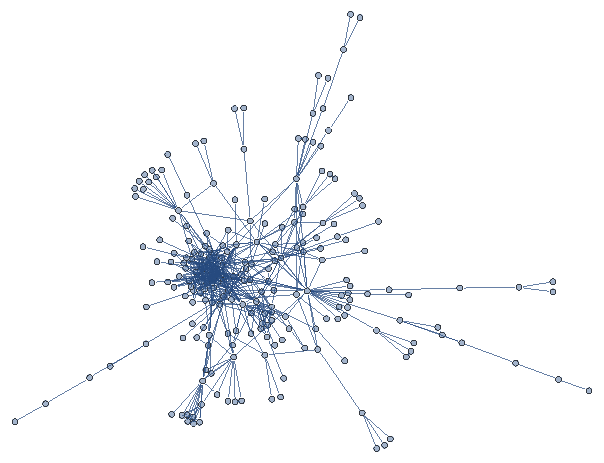
\includegraphics[width=5cm,height=4cm,angle=90]{\networksfigsdir/graph_standard.pdf}
    };
  \end{scope}
  \begin{scope}[xshift=4.5cm]
    \node [mybox] (box){
      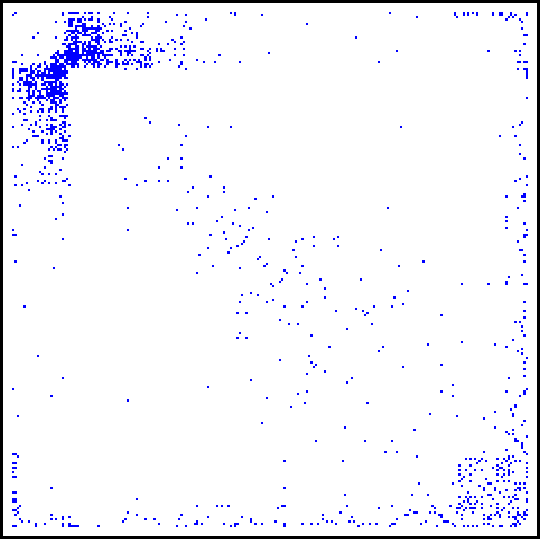
\includegraphics[width=3.5cm]{\networksfigsdir/interactome_adjacency_mathematica.pdf}

  };
  \end{scope}  
  \begin{scope}[xshift=9.2cm]
    \node [mybox] (box){
      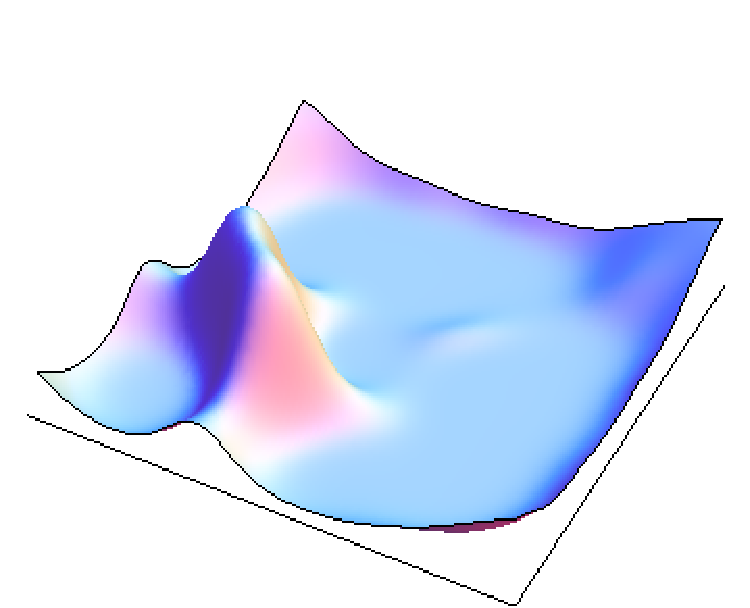
\includegraphics[width=5cm]{\networksfigsdir/graphon_listplot_bmp.pdf}
  };
  \end{scope}
\end{tikzpicture}

  \vspace{-0.5cm}
  \caption{Protein interactome data. 
    \emph{Left:} Interactome network. 
    \emph{Middle:} Sorted adjacency matrix. The network exhibits stochastic equivalence 
    (visible as block structure in the matrix) and homophily (concentration of points around the diagonal). 
    \emph{Right:} Maximum a posteriori estimate of the function $\AHfunction$, corresponding to the function in Fig.~\ref{fig:W:graph} (middle).
  }
  \label{fig:(R)GPLVM_Comparison}
\end{figure}

The sorted adjacency matrix and MAP estimate of $\Theta$ reveal many qualitatively different structures present in the network.
The bottom right of the adjacency matrix reveals a densely connected block of nodes; this is highlighted and visualised in figure~\ref{fig:networks:block}.
In contrast, figure~\ref{fig:networks:sparse} highlights many nodes which display patterns of transitivity although the overall connectivity is sparse.
A pair of hub nodes are also revealed as demonstrated in figure~\ref{fig:networks:hubs}.

\begin{figure}[ht]
  \centering
\begin{tikzpicture}[]
  \begin{scope}[xshift=0.0\textwidth]
    \node [mybox] (box){
      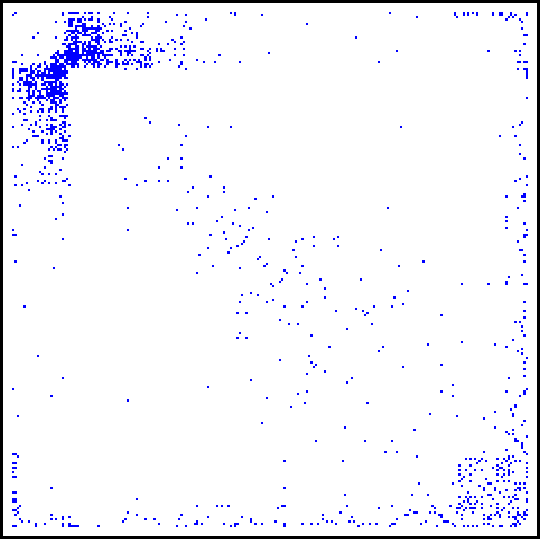
\includegraphics[width=0.45\textwidth]{\networksfigsdir/interactome_adjacency_mathematica.pdf}
    };
    \draw [dashed, ultra thick, red, opacity=0.7] (0.15\textwidth,-0.150\textwidth) -- (0.15\textwidth,-0.22\textwidth) -- (0.220\textwidth,-0.22\textwidth) -- (0.220\textwidth,-0.150\textwidth) -- (0.15\textwidth,-0.150\textwidth);
  \end{scope}  
  \begin{scope}[xshift=0.5\textwidth]
    \node [mybox] (box){
      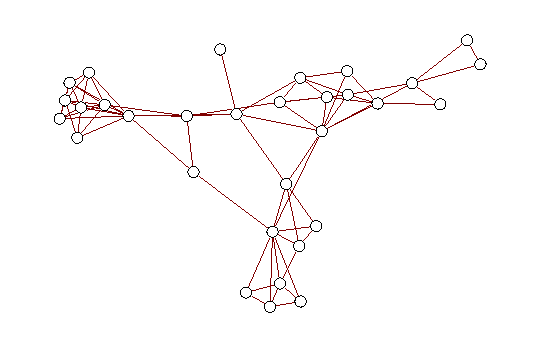
\includegraphics[width=0.45\textwidth]{\networksfigsdir/interactome_clique.pdf}
    };
  \end{scope}
\end{tikzpicture}
  \caption{A densely connected group of nodes in the protein interactome.}
  \label{fig:networks:block}
\end{figure}

\begin{figure}[ht]
  \centering
\begin{tikzpicture}[]
  \begin{scope}[xshift=0.0\textwidth]
    \node [mybox] (box){
      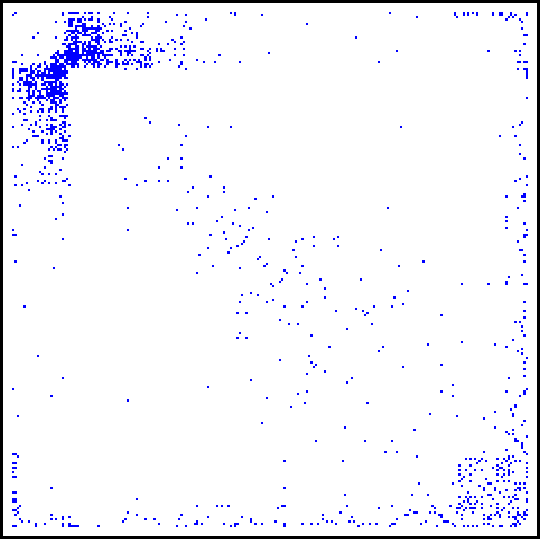
\includegraphics[width=0.45\textwidth]{\networksfigsdir/interactome_adjacency_mathematica.pdf}
    };
    \draw [dashed, ultra thick, red, opacity=0.7] (0.15\textwidth,-0.150\textwidth) -- (0.15\textwidth,+0.1\textwidth) -- (-0.1\textwidth,+0.1\textwidth) -- (-0.1\textwidth,-0.150\textwidth) -- (0.15\textwidth,-0.150\textwidth);
  \end{scope}  
  \begin{scope}[xshift=0.5\textwidth]
    \node [mybox] (box){
      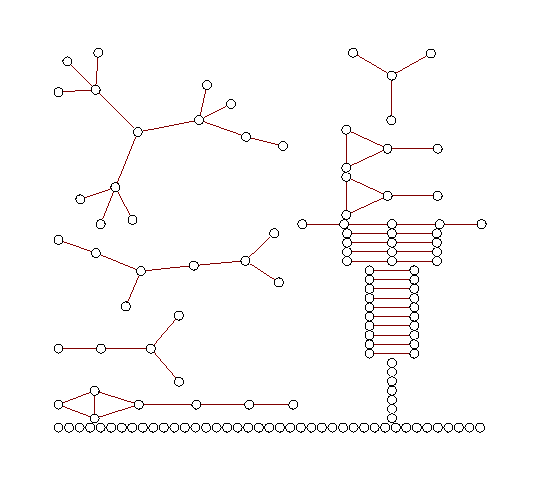
\includegraphics[width=0.45\textwidth]{\networksfigsdir/interactome_sparse.pdf}
    };
  \end{scope}
\end{tikzpicture}
  \caption{Sparsely connected nodes in the protein interactome with some transitivity (triangles).}
  \label{fig:networks:sparse}
\end{figure}

\begin{figure}[ht]
  \centering
\begin{tikzpicture}[]
  \begin{scope}[xshift=0.0\textwidth]
    \node [mybox] (box){
      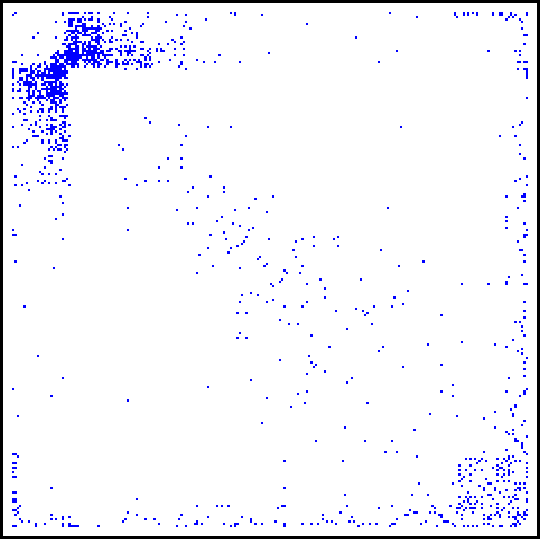
\includegraphics[width=0.45\textwidth]{\networksfigsdir/interactome_adjacency_mathematica.pdf}
    };
    \draw [dashed, ultra thick, red, opacity=0.7] (0.205\textwidth,0.22\textwidth) -- (0.205\textwidth,-0.22\textwidth) -- (0.220\textwidth,-0.22\textwidth) -- (0.220\textwidth,0.22\textwidth) -- (0.205\textwidth,0.22\textwidth);
  \end{scope}  
  \begin{scope}[xshift=0.5\textwidth]
    \node [mybox] (box){
      %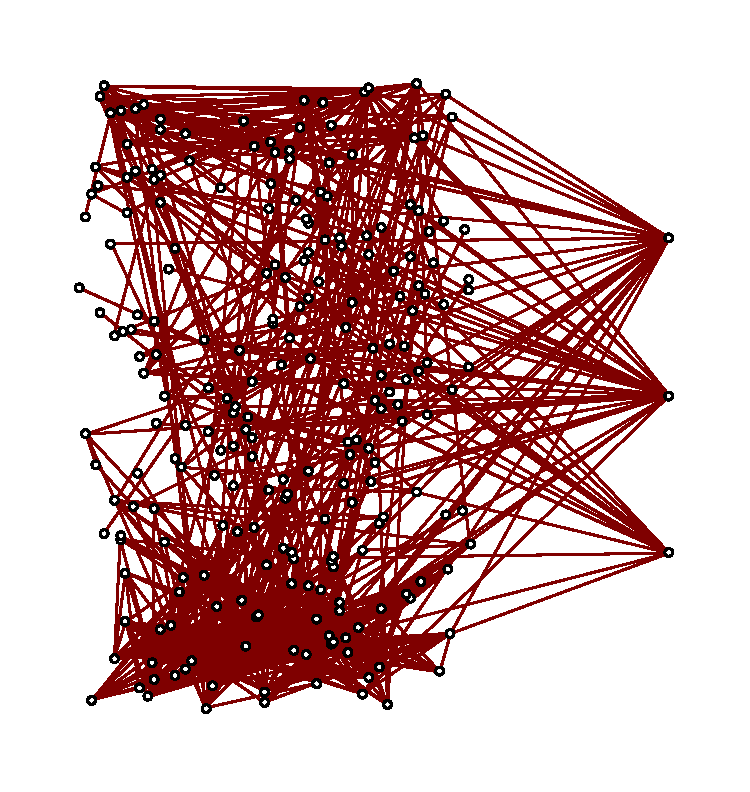
\includegraphics[width=0.45\textwidth]{\networksfigsdir/interactome_hub.pdf}
      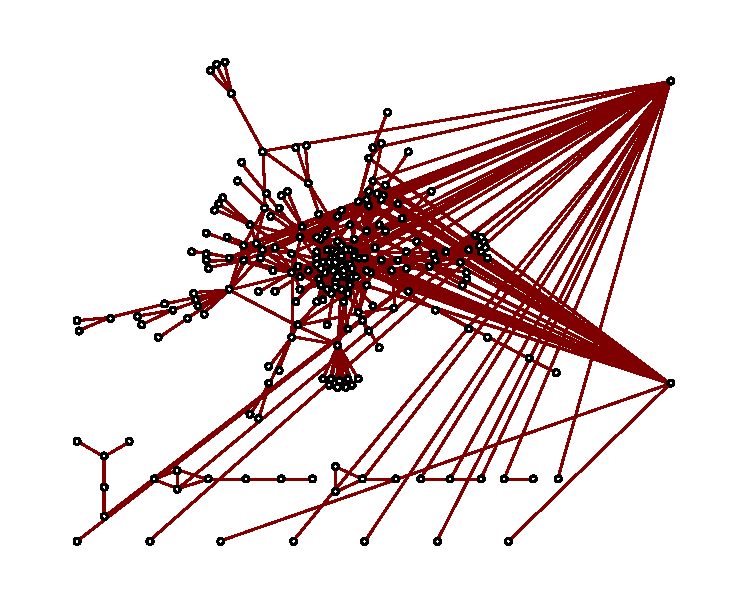
\includegraphics[width=0.45\textwidth]{\networksfigsdir/two_hub.pdf}
    };
  \end{scope}
\end{tikzpicture}
  \caption{Two hub nodes in the protein interactome.}
  \label{fig:networks:hubs}
\end{figure}

Finally, the prominent feature at the top left of the adjacency matrix is visualised in figure~\ref{fig:networks:butterfly}.
The sorted adjacency matrix has revealed three blocks of nodes which we will refer to as the left, right and top blocks according to the right hand side of figure~\ref{fig:networks:butterfly}.
Ignoring the top block, the left and right blocks are nearly bipartite.
The top block is almost a clique and is much more strongly connected to the right block than the left.
The degree distribution of the left and right blocks is also of interest; the variation is larger than expected by a block model (assuming that the probability of a link between different blocks is constant).
A more detailed analysis is currently ongoing, but the structure found by this analysis can be shown to correspond with reality; for example, the proteins on the left are almost all ribosomal subunits.

\begin{figure}[ht]
  \centering
\begin{tikzpicture}[]
  \begin{scope}[xshift=0.0\textwidth]
    \node [mybox] (box){
      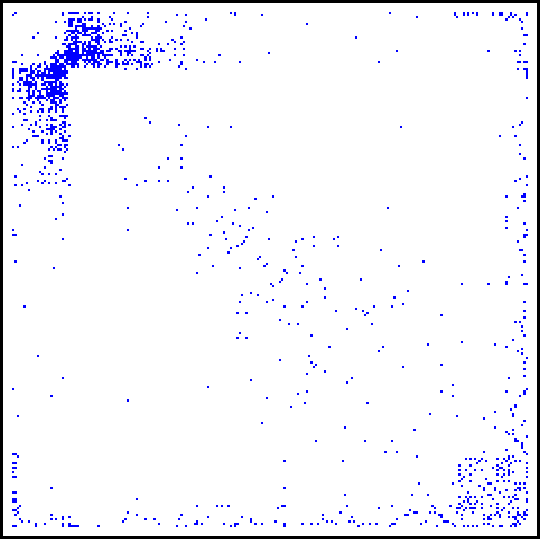
\includegraphics[width=0.45\textwidth]{\networksfigsdir/interactome_adjacency_mathematica.pdf}
    };
    \draw [dashed, ultra thick, red, opacity=0.7] (-0.22\textwidth,+0.220\textwidth) -- (-0.22\textwidth,+0.1\textwidth) -- (-0.1\textwidth,+0.1\textwidth) -- (-0.1\textwidth,+0.22\textwidth) -- (-0.22\textwidth,+0.220\textwidth);
    \draw [dotted, ultra thick, red, opacity=0.9] (-0.185\textwidth,+0.185\textwidth) -- (-0.185\textwidth,+0.16\textwidth) -- (-0.16\textwidth,+0.16\textwidth) -- (-0.16\textwidth,+0.185\textwidth) -- (-0.185\textwidth,+0.185\textwidth);
  \end{scope}  
  \begin{scope}[xshift=0.5\textwidth]
    \node [mybox] (box){
      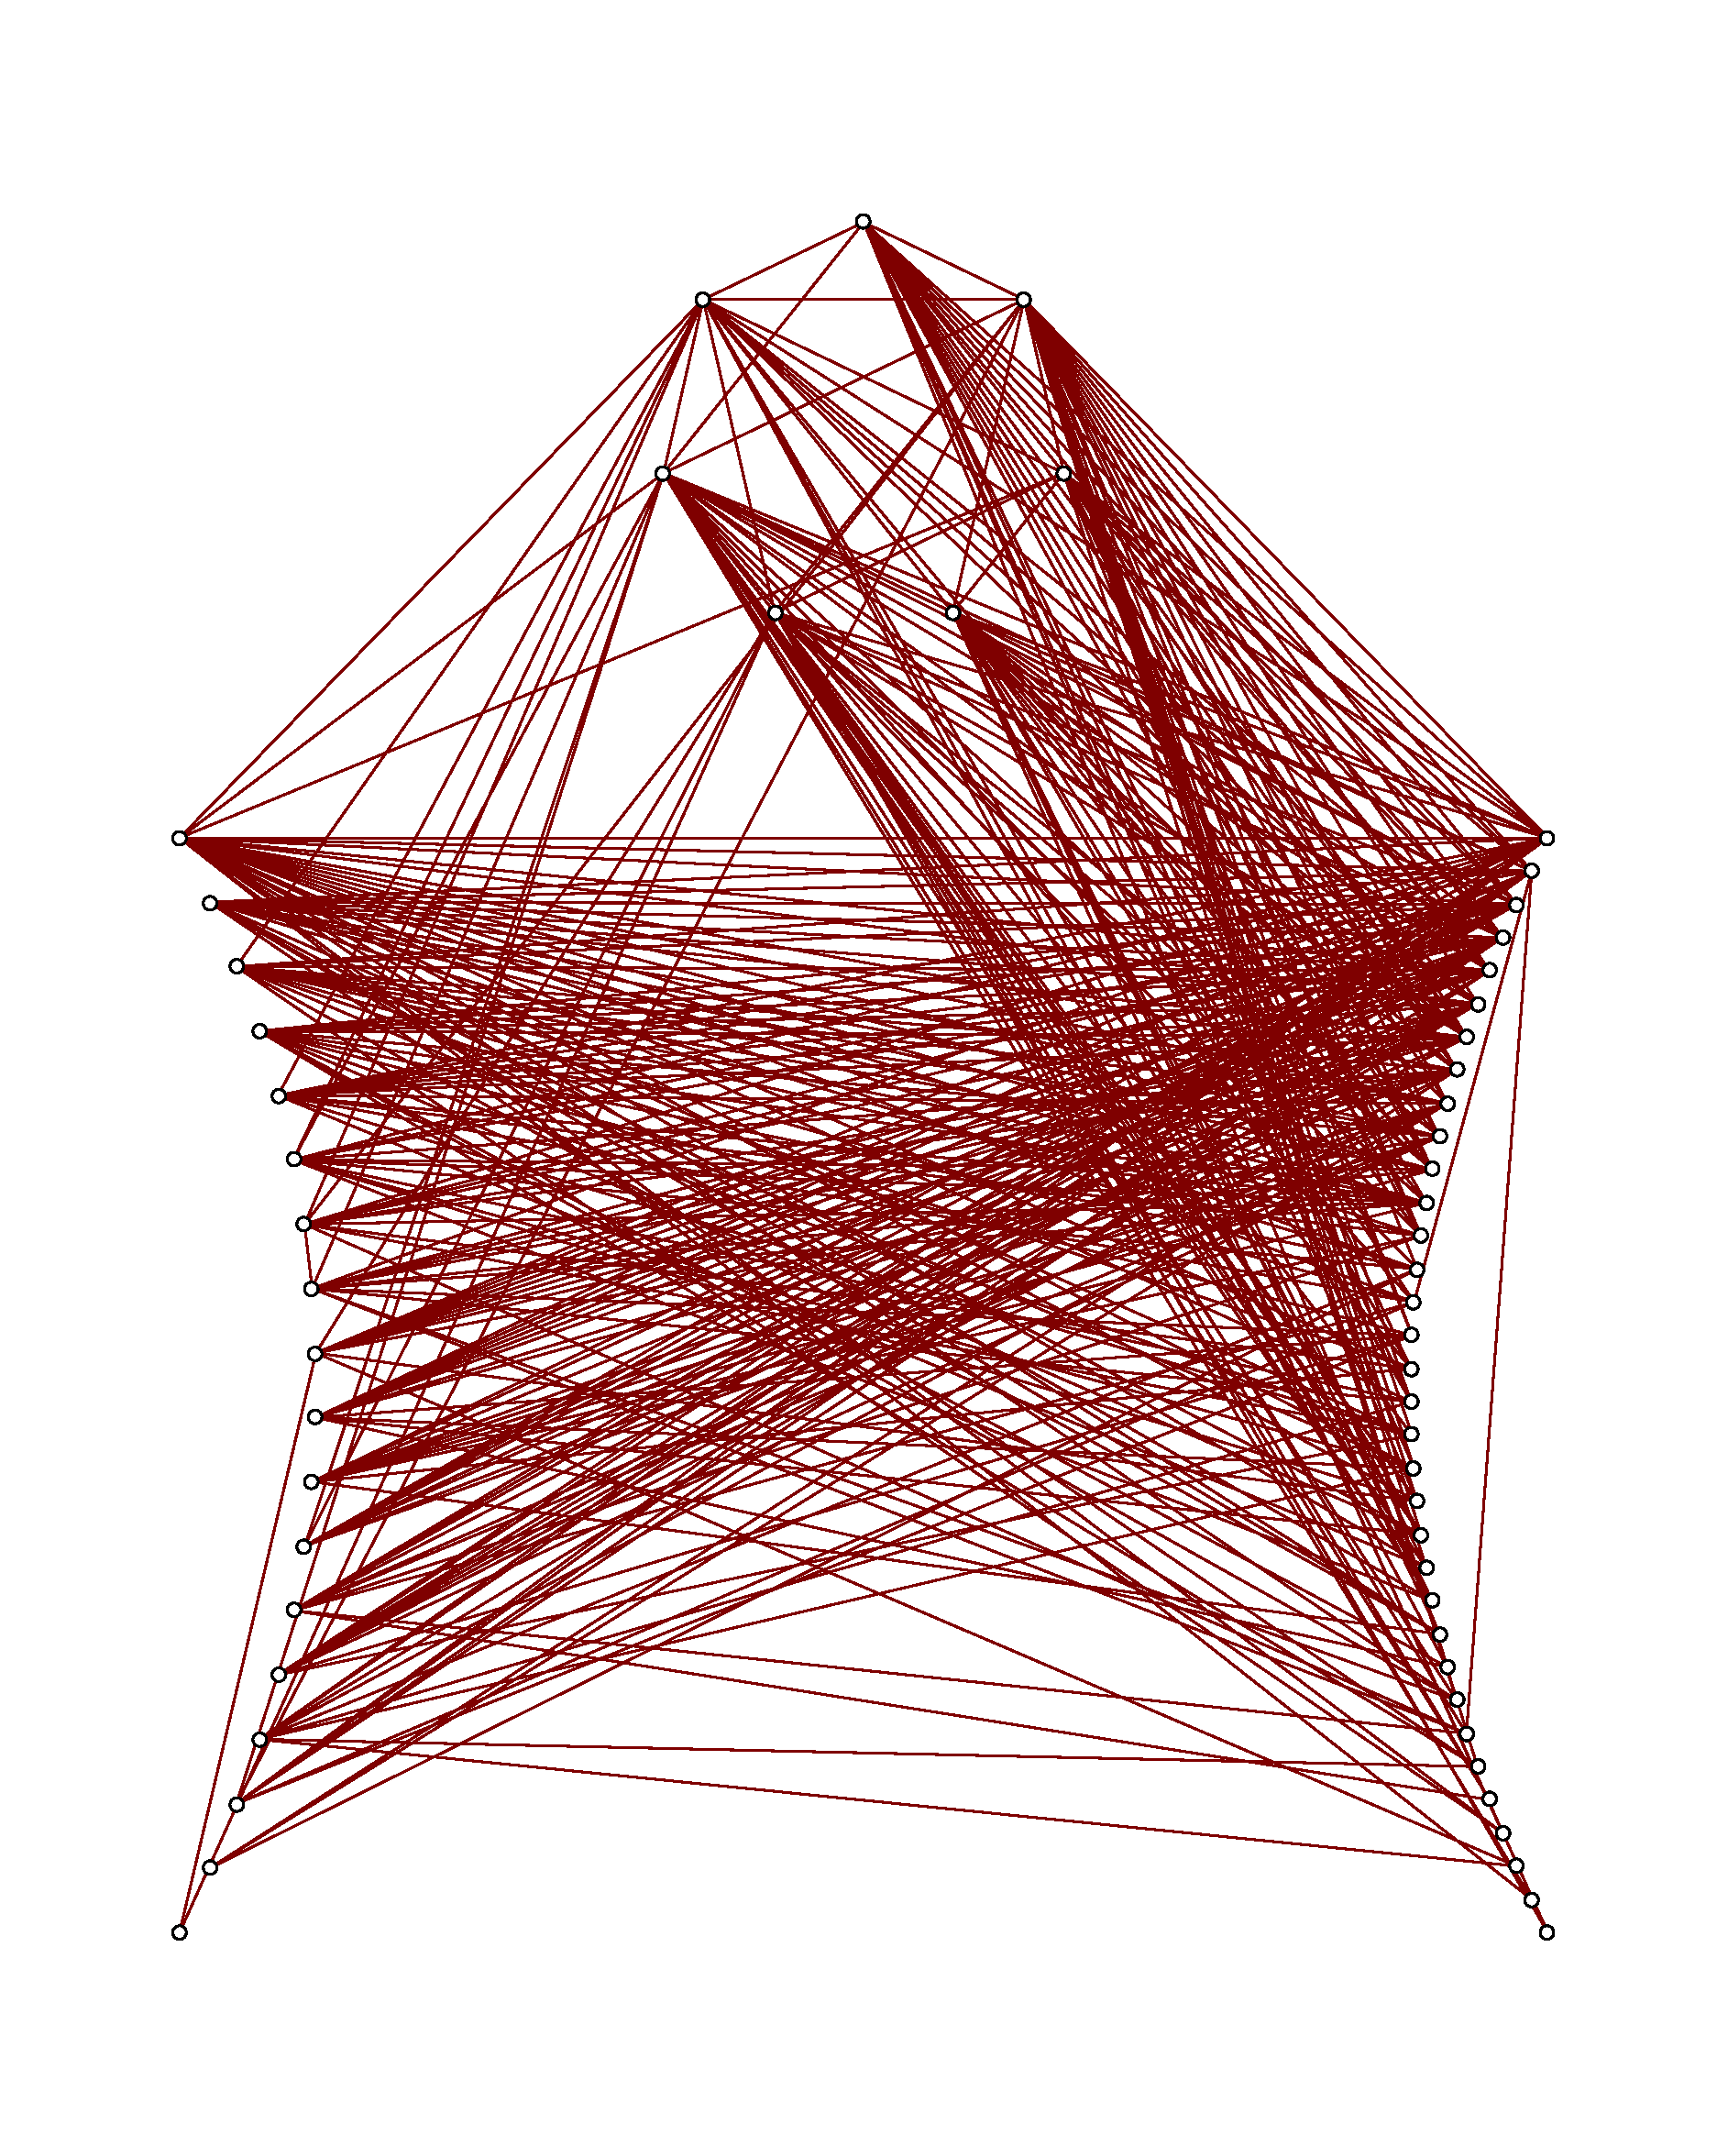
\includegraphics[width=0.45\textwidth]{\networksfigsdir/butterfly.pdf}
    };
  \end{scope}
\end{tikzpicture}
  \caption{Three groups of nodes in the protein interactome with an interesting connectivity pattern.}
  \label{fig:networks:butterfly}
\end{figure}

Similar but less complicated structures are observed in the NIPS and Highschool datasets.
Figure~\ref{fig:networks:nips} shows unsorted (left) and sorted (right) adjacency matrices for the NIPS coauthorship network.
The map embedding of the $U_i$ has identified clear block structures of densely connected groups of authors.\fTBD{Try to comment on these blocks}
However, there are many authors (in the middle of the adjacency matrix) for which there is no block structure, only transitivity (coauthors of coauthors are likely to be coauthors).
Similarly, the sorted high school social network adjacency matrix in figure~\ref{fig:networks:highschool} mostly shows patterns of transitivity with most links along the diagonal.

\begin{figure}[ht]
  \centering
  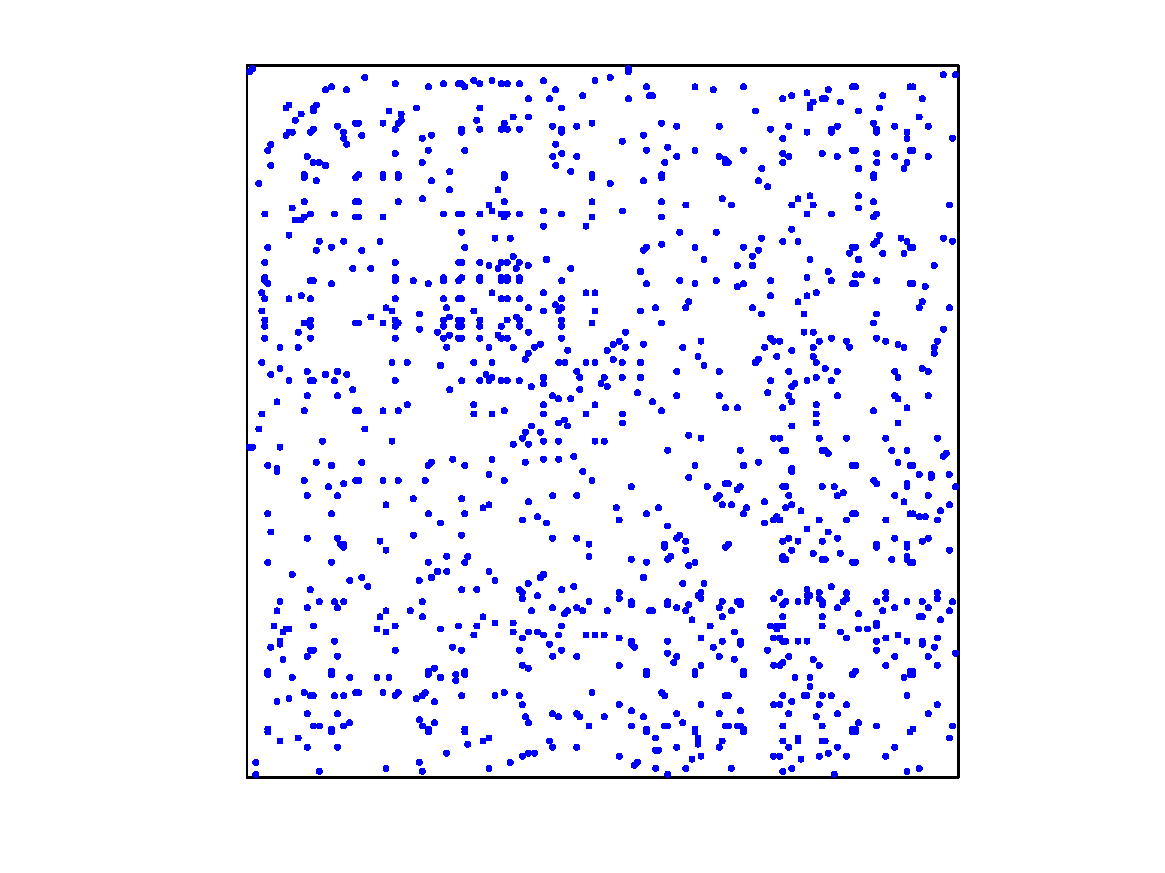
\includegraphics[width=0.45\textwidth]{\networksfigsdir/nips_unsorted}
  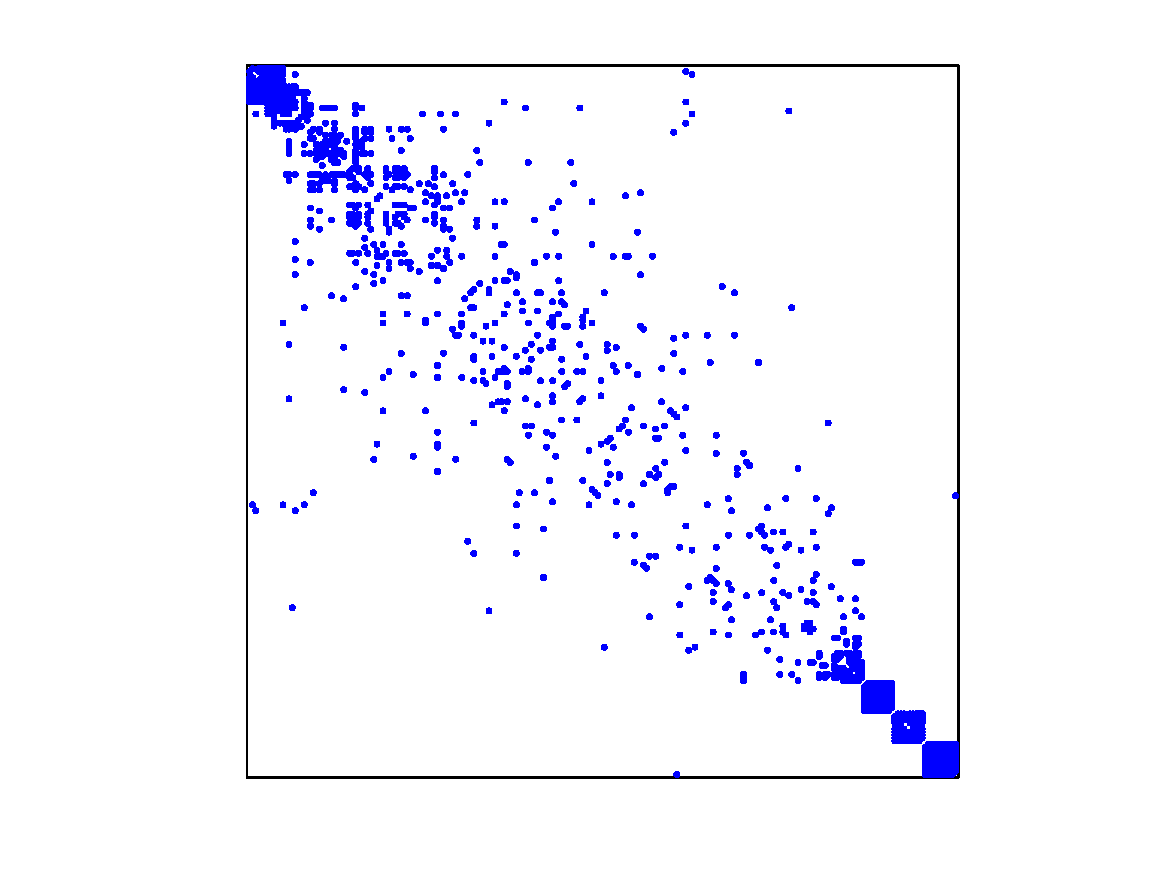
\includegraphics[width=0.45\textwidth]{\networksfigsdir/nips_sorted}
  \caption{NIPS coauthorship data. 
    \emph{Left:} Unsored adjacency matrix. 
    \emph{Middle:} Sorted adjacency matrix.
  }
  \label{fig:networks:nips}
\end{figure}

\begin{figure}[ht]
  \centering
  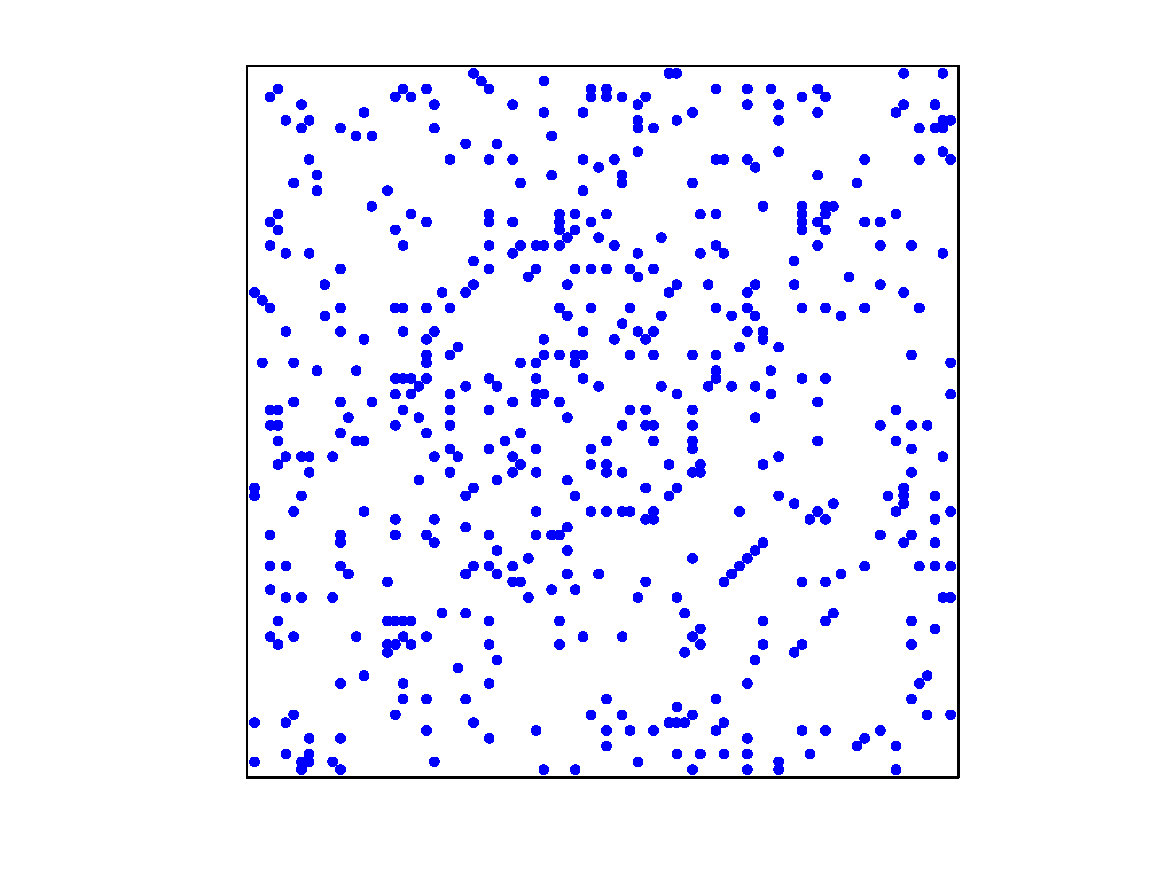
\includegraphics[width=0.45\textwidth]{\networksfigsdir/highschool_unsorted}
  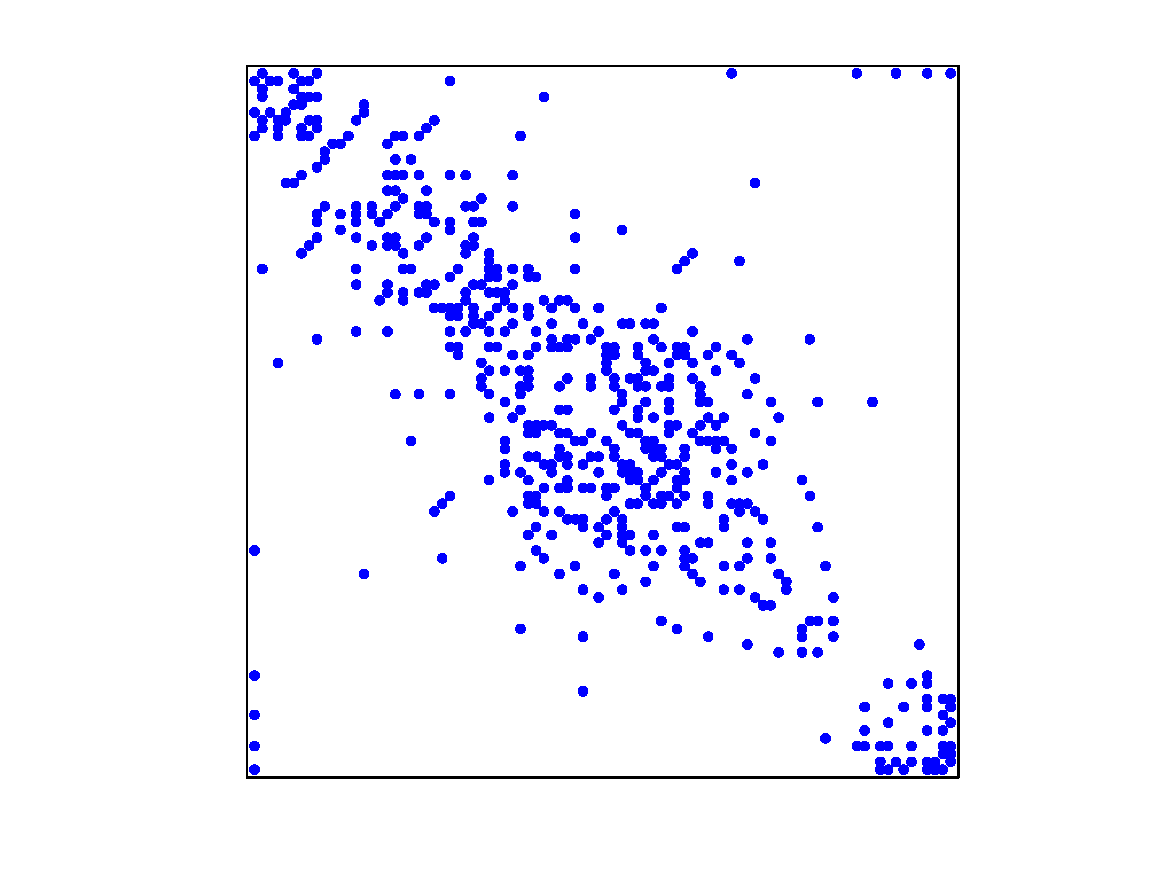
\includegraphics[width=0.45\textwidth]{\networksfigsdir/highschool_sorted}
  \caption{Highschool social network. 
    \emph{Left:} Unsored adjacency matrix. 
    \emph{Middle:} Sorted adjacency matrix.
  }
  \label{fig:networks:highschool}
\end{figure}

%\begin{rem}[Model complexity and lengthscales]
%\label{rem:lengthscale}  
%\fTBD{Needs review}
%Figure~\ref{fig:(R)GPLVM_Comparison} provides a visualisation of $\AHfunction$ when modelling the protein interactome data using 1 latent dimension.
%The most prominent feature of the plot is the smooth peak in the top left of the adjacency matrix.
%The likelihood of such a feature is sensitive to the lengthscale of the Gaussian process representation of $\AHfunction$; smaller lengthscales will encourage more complex functions and vice versa.
%It was noted in section~\ref{sec:Model} that the choice of a Gaussian process prior introduces the assumption that $\AHfunction$ is continuous.
%However, continuous functions are dense in the space of measurable functions, \ie any measurable function can be arbitrarily well approximated by a continuous one.
%The assumption of continuity is therefore not restrictive, but rather the lengthscale of the Gaussian process determines the complexity of the model a priori.
%The nonparametric prior placed on $\AHfunction$ allows the posterior to approximate any function if supported by the data, but by sampling the lengthscale we allow the model to quickly select an appropriate level of complexity.
%\end{rem}

\section{Discussion and conclusions}

There has been a tremendous amount of research into modelling matrices, arrays, graphs and relational data, but nonparametric
Bayesian modeling of such data has only recently been explored.
In most modelling circumstances, the assumption of exchangeability amongst data objects is natural and fundamental to the model.
In this case, the representation results 
\citep{Aldous1981-lg,Hoover1979-br,Kallenberg1992-gb} 
precisely map out the scope of possible probabilistic models for exchangeable arrays:
Any such model can be interpreted as a prior on random measurable functions on a suitable space.

Nonparametric Bayesian statistics provides a number of possible priors on random functions, but the Gaussian process
and its modifications are the only well-studied model for almost surely continuous functions.
For this choice of prior, our work provides a general and simple modelling approach that can be motivated directly by the
relevant representation results.
%Inference is then possible using an efficient MCMC algorithm for this model. 
The model results in both interpretable representations for networks, such as a visualisation of a protein interactome, and has 
competitive predictive performance on benchmark data.

%% There has been a tremendous amount of research into modelling matrices, arrays, graphs and relational data. 
%% In most modelling circumstances, the assumption of exchangeability amongst data objects is natural and fundamental to the model.
%% One of the contributions of this paper is to highlight fundamental results in probability theory that justify the use of latent variable models for exchangeable arrays, especially when one employs a nonparametric prior over the functions mapping from latent variables to data. We have also related our work to many other models for graphs and matrices.

%% In this paper we have used a Gaussian process prior to model random functions and have developed an efficient MCMC algorithm for this model. In doing so we have created an MCMC variant of a widely used sparse approximation for Gaussian processes.
%% Our model results in both interpretable representations for networks, such as a visualisation of a protein interactome, and has competitive predictive performance on three benchmark data sets.

\outbpdocument{
\bibliographystyle{plainnat}
\bibliography{references.bib}
}

%
% A header that lets you compile a chapter by itself, or inside a larger document.
% Adapted from stackoverflow.com/questions/3655454/conditional-import-in-latex
%
%
%Use \inbpdocument and \outbpdocument in your individual files, in place of \begin{document} and \end{document}. In your main file, put in a \def \ismaindoc {} before including or importing anything.
%
% David Duvenaud
% June 2011
% 
% ======================================
%
%


\ifx\ismaindoc\undefined
	\newcommand{\inbpdocument}{
		\def \ismaindoc {}
		% Use this header if we are compiling by ourselves.
		\documentclass[a4paper,11pt,authoryear,index]{common/PhDThesisPSnPDF}
		
%\usepackage{draftwatermark}
%\SetWatermarkLightness{0.95}

% ******************************************************************************
% ****************************** Custom Margin *********************************

% Add `custommargin' in the document class options to use this section
% Set {innerside margin / outerside margin / topmargin / bottom margin}  and
% other page dimensions

\ifsetMargin
\else
    \RequirePackage[left=37mm,right=30mm,top=35mm,bottom=30mm]{geometry}
    \setFancyHdr % To apply fancy header after geometry package is loaded
\fi


%\chead{Unfinished draft}
%\cfoot{\texttt{Unfinished draft - compiled on \today{} at \currenttime}}

% *****************************************************************************
% ******************* Fonts (like different typewriter fonts etc.)*************

% Add `customfont' in the document class option to use this section

\ifsetFont
\else
    % Set your custom font here and use `customfont' in options. Leave empty to
    % load computer modern font (default LaTeX font).  

    \RequirePackage{libertine} 
\fi

% *****************************************************************************
% *************************** Bibliography  and References ********************

%\usepackage{cleveref} %Referencing without need to explicitly state fig /table

% Add `custombib' in the document class option to use this section
\ifsetBib % True, Bibliography option is chosen in class options
\else % If custom bibliography style chosen then load bibstyle here

   \RequirePackage[square, sort, numbers, authoryear]{natbib} % CustomBib

% If you would like to use biblatex for your reference management, as opposed to the default `natbibpackage` pass the option `custombib` in the document class. Comment out the previous line to make sure you don't load the natbib package. Uncomment the following lines and specify the location of references.bib file

% \RequirePackage[backend=biber, style=numeric-comp, citestyle=numeric, sorting=nty, natbib=true]{biblatex}
% \bibliography{References/references} %Location of references.bib only for biblatex

\fi


% changes the default name `Bibliography` -> `References'
\renewcommand{\bibname}{References}


% *****************************************************************************
% *************** Changing the Visual Style of Chapter Headings ***************
% Uncomment the section below. Requires titlesec package.

%\RequirePackage{titlesec}
%\newcommand{\PreContentTitleFormat}{\titleformat{\chapter}[display]{\scshape\Large}
%{\Large\filleft{\chaptertitlename} \Huge\thechapter}
%{1ex}{}
%[\vspace{1ex}\titlerule]}
%\newcommand{\ContentTitleFormat}{\titleformat{\chapter}[display]{\scshape\huge}
%{\Large\filleft{\chaptertitlename} \Huge\thechapter}{1ex}
%{\titlerule\vspace{1ex}\filright}
%[\vspace{1ex}\titlerule]}
%\newcommand{\PostContentTitleFormat}{\PreContentTitleFormat}
%\PreContentTitleFormat


% *****************************************************************************
% **************************** Custom Packages ********************************
% *****************************************************************************


% ************************* Algorithms and Pseudocode **************************

%\usepackage{algpseudocode} 


% ********************Captions and Hyperreferencing / URL **********************

% Captions: This makes captions of figures use a boldfaced small font. 
%\RequirePackage[small,bf]{caption}

\RequirePackage[labelsep=space,tableposition=top]{caption} 
%\renewcommand{\figurename}{Figure} %to support older versions of captions.sty
\captionsetup{labelsep = colon,belowskip=12pt,aboveskip=4pt}

% ************************ Formatting / Footnote *******************************

%\usepackage[perpage]{footmisc} %Range of footnote options 


% ****************************** Line Numbers **********************************

%\RequirePackage{lineno}
%\linenumbers

% ************************** Graphics and figures *****************************

%\usepackage{rotating}
%\usepackage{wrapfig}
%\usepackage{float}
\usepackage{subfig} %note: subfig must be included after the `caption` package. 


% ********************************* Table **************************************

%\usepackage{longtable}
%\usepackage{multicol}
%\usepackage{multirow}
%\usepackage{tabularx}


% ***************************** Math and SI Units ******************************

\usepackage{amsfonts}
\usepackage{amsmath}
\usepackage{amssymb}
%\usepackage{siunitx} % use this package module for SI units


% ******************************************************************************
% ************************* User Defined Commands ******************************
% ******************************************************************************

% *********** To change the name of Table of Contents / LOF and LOT ************

%\renewcommand{\contentsname}{My Table of Contents}
%\renewcommand{\listfigurename}{List of figures}
%\renewcommand{\listtablename}{List of tables}


% ********************** TOC depth and numbering depth *************************

\setcounter{secnumdepth}{2}
\setcounter{tocdepth}{2}

% ******************************* Nomenclature *********************************

% To change the name of the Nomenclature section, uncomment the following line

%\renewcommand{\nomname}{Symbols}


% ********************************* Appendix ***********************************

% The default value of both \appendixtocname and \appendixpagename is `Appendices'. These names can all be changed via: 

%\renewcommand{\appendixtocname}{List of appendices}
%\renewcommand{\appendixname}{Appndx}

		% All my custom preamble stuff.  Shouldn't overlap with anything in official-preamble




% Paths to figure and table directories.
\newcommand{\symmetryfigsdir}{figures/symmetries}
\newcommand{\topologyfiguresdir}{figures/topology}
\newcommand{\infinitefiguresdir}{figures/infinite}
\newcommand{\grammarfiguresdir}{figures/grammar}
\newcommand{\introfigsdir}{figures/intro}
\newcommand{\gplvmfiguresdir}{figures/gplvm}
\newcommand{\warpedfiguresdir}{figures/warped-mixtures}
\newcommand{\deeplimitsfiguresdir}{figures/deep-limits}
\newcommand{\quadraturefigsdir}{figures/quadrature}
\newcommand{\additivefigsdir}{figures/additive}
\newcommand{\decompfigsdir}{figures/decomp}
\newcommand{\examplefigsdir}{figures/worked-example}

\usepackage{bm}  % for warped mixtures - is this necessary?
\usepackage{booktabs}
\usepackage{tabularx}
\usepackage{multirow}
\usepackage{datetime}
\renewcommand{\tabularxcolumn}[1]{>{\arraybackslash}m{#1}}
\usepackage{relsize}
\usepackage{graphicx}
\usepackage{amsmath,amssymb,textcomp}
\usepackage{nicefrac}
\usepackage{amsthm}
\usepackage{tikz}
\usetikzlibrary{arrows}
\usetikzlibrary{calc}
\usepackage{nth}
\usepackage{rotating}
\usepackage{array}
\usepackage{fp}
\usepackage{cleveref}   % Note: this package sometimes causes the page counter to reset.
\crefname{equation}{equation}{equations}
\crefname{figure}{figure}{figures}
%\usepackage{common/sectsty}

% Controls capitalization of all headers
%\usepackage{stringstrings}
%\usepackage[explicit]{titlesec}
%\newcommand\SentenceCase[1]{%
%  \caselower[e]{#1}%
%  \capitalize[q]{\thestring}%
%}
%\titleformat{\section}
%  {\normalfont\Large\bfseries}{\thesection}{1em}{\SentenceCase{#1}\thestring}


%\titleformat{\section} % The normal, unstarred version
%    {\Large\bfseries}{}{2ex}
%    {\thesection. \MakeSentenceCase{#1}}

%\titleformat{name=\section,numberless} % The starred version; note the `numberless` key
%    {\Large\bfseries}{}{2ex}
%    {\MakeSentenceCase{#1}}

\usepackage[hyperpageref]{backref}
% Setup to show (pages 4 and 9) sort of thing in the bibliography - DD
%\def\foo{\hspace{\fill}\mbox{}\linebreak[0]\hspace*{\fill}}
%\def\foo{\parbox{3cm}{\hfill}
%\def\foo{\parbox{3cm}{\hfill}
%\newcommand\foo[1]{{\raggedleft{\hfill{\mbox{\hfill{#1}}}}}}
\newcommand{\comfyfill}[1]{% = Thorsten Donig's \signed
  \unskip\hspace*{0.1em plus 1fill}
  \nolinebreak[3]%
  \hspace*{\fill}\mbox{#1}
  \parfillskip0pt\par
}
\newcommand\foo[1]{{\comfyfill{\mbox{#1}}}}
%\newcommand\foo[1]{{\mbox{#1}}}
\renewcommand*{\backref}[1]{}
\renewcommand*{\backrefalt}[4]{%
\ifcase #1 %
%
\or
\foo{(page #2)}%
\else
\foo{(pages #2)}%
\fi
}

\usepackage{stringstrings}

%\newcommand{\headercase}{\
%\DeclareFieldFormat{titlecase}{\MakeSentenceCase{#1}}


%% For submission, make all render blank.
\input{common/commenting.tex}
%\renewcommand{\LATER}[1]{}
%\renewcommand{\fLATER}[1]{}
%\renewcommand{\TBD}[1]{}
%\renewcommand{\fTBD}[1]{}
%\renewcommand{\PROBLEM}[1]{}
%\renewcommand{\fPROBLEM}[1]{}
%\renewcommand{\NA}[1]{}


% HUMBLE WORDS: shown slightly smaller when in normal text
% Thanks to Christian Steinruecken!
\input{common/humble.tex}


% TODO: Clean up duplicates
\declareHumble{ANOVA}{ANOVA}
\declareHumble{ARD}{ARD}
\declareHumble{BIC}{BIC}
\declareHumble{BMC}{BMC}
\declareHumble{bq}{BQ}
\declareHumble{CRP}{CRP}
\declareHumble{dirpro}{DP}
\declareHumble{HDMR}{HDMR}
\declareHumble{GAM}{GAM}
\declareHumble{GEM}{GEM}
\declareHumble{GMM}{GMM}
\declareHumble{gplvm}{GP-LVM}
\declareHumble{gpml}{GPML}
\declareHumble{GPML}{GPML}
\declareHumble{gprn}{GPRN}
\declareHumble{gpt}{GP}
\declareHumble{gp}{GP}
\declareHumble{HKL}{HKL}
\declareHumble{HMC}{HMC}
\declareHumble{ibp}{IBP}
\declareHumble{iGMM}{iGMM}
\declareHumble{iwmm}{iWMM}
\declareHumble{kCP}{CP}
\declareHumble{kCW}{CW}
\declareHumble{kC}{C}
\declareHumble{KDE}{KDE}
\declareHumble{kLin}{Lin}
\declareHumble{KPCA}{KPCA}
\declareHumble{kPer}{Per}
\declareHumble{kPerGen}{ZMPer}
\declareHumble{kRQ}{RQ}
\declareHumble{kSE}{SE}
\declareHumble{kWN}{WN}
\declareHumble{Lin}{Lin}
\declareHumble{LBFGS}{L-BFGS}
\declareHumble{LIBSVM}{LIBSVM}
\declareHumble{MAP}{MAP}
\declareHumble{mcmc}{MCMC}
\declareHumble{MKL}{MKL}
\declareHumble{MLP}{MLP}
\declareHumble{MNIST}{MNIST}
\declareHumble{MSE}{MSE}
\declareHumble{OU}{OU}
\declareHumble{Per}{Per}
\declareHumble{RBF}{RBF}
\declareHumble{RMSE}{RMSE}
\declareHumble{RQ}{RQ}
\declareHumble{SBQ}{SBQ}
\declareHumble{seard}{SE-ARD}
\declareHumble{sefull}{SE-\textnormal{full}}
\declareHumble{SEGP}{SE-GP}
\declareHumble{SE}{SE}
\declareHumble{SNR}{SNR}
\declareHumble{SSANOVA}{SS-ANOVA}
\declareHumble{SVM}{SVM}
\declareHumble{UCI}{UCI}
\declareHumble{UMIST}{UMIST}
\declareHumble{vbgplvm}{VB GP-LVM}

\newcommand{\kSig}{\boldsymbol\sigma}

\def\subexpr{{\cal S}}
\def\baseker{{\cal B}}
\def\numWinners{k}

\def\ie{i.e.\ }
\def\eg{e.g.\ }
\def\etc{etc.\ }
\let\oldemptyset\emptyset
%\let\emptyset 0




% Unify notation between neural-net land and GP-land.
\newcommand{\hphi}{h}
\newcommand{\hPhi}{\vh}
\newcommand{\walpha}{w}
\newcommand{\wboldalpha}{\bw}
\newcommand{\wcapalpha}{\vW}
\newcommand{\lengthscale}{w}

\newcommand{\layerindex}{\ell}



\newcommand{\gpdrawbox}[1]{
\setlength\fboxsep{0pt}
\hspace{-0.15in} 
\fbox{
\includegraphics[width=0.464\columnwidth]{\deeplimitsfiguresdir/deep_draws/deep_gp_sample_layer_#1}
}}



\newcommand{\procedurename}{ABCD}
\newcommand{\genText}[1]{{\sf #1}}



\newcommand{\asdf}{$^{\textnormal{th}}$}

\newcommand{\binarysum}{\sum_{\bf{x} \in \{0,1\}^D}}
\newcommand{\expect}{\mathbb{E}}
\newcommand{\expectargs}[2]{\mathbb{E}_{#1} \left[ {#2} \right]}
\newcommand{\var}{\mathbb{V}}
\newcommand{\varianceargs}[2]{\mathbb{V}_{#1} \left[ {#2} \right]}
\newcommand{\cov}{\operatorname{cov}}
\newcommand{\Cov}{\operatorname{Cov}}
\newcommand{\covargs}[2]{\Cov \left[ {#1}, {#2} \right]}
\newcommand{\variance}{\mathbb{V}}
\newcommand{\vecop}[1]{\operatorname{vec} \left( {#1} \right)}

\newcommand{\covarianceargs}[2]{\Cov_{#1} \left[ {#2} \right]}
\newcommand{\colvec}[2]{\left[ \begin{array}{c} {#1} \\ {#2} \end{array} \right]}
\newcommand{\tbtmat}[4]{\left[ \begin{array}{cc} {#1} & {#2} \\ {#3} & {#4} \end{array} \right]}

\newcommand{\acro}[1]{{\humble{#1}}}
%\newcommand{\vect}[1]{\boldsymbol{#1}}
\newcommand{\vect}[1]{{\bf{#1}}}
\newcommand{\mat}[1]{\mathbf{#1}}
\newcommand{\pderiv}[2]{\frac{\partial #1}{\partial #2}}
\newcommand{\npderiv}[2]{\nicefrac{\partial #1}{\partial #2}}

\newcommand{\pha}{^{\phantom{:}}}

\newcommand{\argmin}{\operatornamewithlimits{argmin}}
\newcommand{\argmax}{\operatornamewithlimits{argmax}}

% The following designed for probabilities with long arguments

\newcommand{\Prob}[2]{P\!\left(\,#1\;\middle\vert\;#2\,\right)}
\newcommand{\ProbF}[3]{P\!\left(\,#1\!=\!#2\;\middle\vert\;#3\,\right)}
\newcommand{\p}[2]{p\!\left(#1\middle\vert#2\right)}
\newcommand{\po}[1]{p\!\left(#1\right)}
\newcommand{\pF}[3]{p\!\left(\,#1\!=\!#2\;\middle\vert\;#3\,\right)} 
\newcommand{\mean}[2]{{m}\!\left(#1\middle\vert#2\right)}



\newcommand{\valpha}{\boldsymbol{\alpha}}
\newcommand{\va}{\vect{a}}
\newcommand{\vA}{\vect{A}}
\newcommand{\vB}{\mat{B}}
\newcommand{\vb}{\vect{b}}
\newcommand{\vC}{\mat{C}}
\newcommand{\vc}{\vect{c}}
\newcommand{\vecf}{\boldsymbol{f}}
\newcommand{\vell}{\vect{\ell}}
\newcommand{\vepsilon}{\boldsymbol{\epsilon}}
\newcommand{\veps}{\boldsymbol{\epsilon}}
\newcommand{\ve}{\boldsymbol{\epsilon}}
\newcommand{\vf}{\vecf}
\newcommand{\vg}{\vect{g}}
\newcommand{\vh}{\vect{h}}
\newcommand{\vI}{\mat{I}}
\newcommand{\vK}{\mat{K}}
\newcommand{\vk}{\vect{k}}
\newcommand{\vL}{\mat{L}}
\newcommand{\vl}{\vect{l}}
\newcommand{\vmu}{{\boldsymbol{\mu}}}
\newcommand{\vone}{\vect{1}}
\newcommand{\vphi}{{\boldsymbol{\phi}}}
\newcommand{\vpi}{{\boldsymbol{\pi}}}
\newcommand{\vq}{\vect{q}}
\newcommand{\vR}{\mat{R}}
\newcommand{\vr}{\vect{r}}
\newcommand{\vsigma}{{\boldsymbol{\sigma}}}
\newcommand{\vSigma}{\mat{\Sigma}}
\newcommand{\vS}{\mat{S}}
\newcommand{\vs}{\vect{s}}
\newcommand{\vtheta}{{\boldsymbol{\theta}}}
\newcommand{\vu}{\vect{u}}
\newcommand{\vV}{\mat{V}}
\newcommand{\vW}{\mat{W}}
\newcommand{\vw}{\vect{w}}
\newcommand{\vX}{\mat{X}}
\newcommand{\vx}{\vect{x}}
\newcommand{\vY}{\mat{Y}}
\newcommand{\vy}{\vect{y}}
\newcommand{\vzero}{\vect{0}}
\newcommand{\vZ}{\mat{Z}}
\newcommand{\vz}{\vect{z}}


% deep gp notation
\newcommand{\netweights}{w}
\newcommand{\vnetweights}{\vw}
\newcommand{\mnetweights}{\vW}
\newcommand{\outweights}{\v}
\newcommand{\voutweights}{\vv}
\newcommand{\moutweights}{\vV}

\newcommand{\unitparams}{\v}
\newcommand{\vunitparams}{\vv}
\newcommand{\munitparams}{\vV}


\newcommand{\He}{\mathcal{H}}
\newcommand{\normx}[2]{\left\|#1\right\|_{#2}}
\newcommand{\Hnorm}[1]{\normx{#1}{\He}}
\newcommand{\mmd}{{\rm MMD}}


\newcommand{\mf}{\bar{\vf}}

%\newcommand{\mf}{\mu} %{\bar{\ell}}
\newcommand{\lf}{f} % Likelihood function
\newcommand{\st}{_\star}

% from simpler log-bq writeup
\newcommand{\lftwo}{{\log \ell}}
\newcommand{\mftwo}{{\bar \ell}}
\newcommand{\loggp}{{\log\acro{GP}}}%| \bX, \vy )}}
\newcommand{\loggpdist}{{\acro{GP}(\lftwo)}}%| \vX, \vy )}}


\newcommand{\inv}{^{{\mathsmaller{-1}}}}
\newcommand{\tohalf}{^{{\mathsmaller{\nicefrac{1}{2}}}}}

\newcommand{\Normal}{\mathcal{N}}
\newcommand{\N}[3]{\mathcal{N}\!\left(#1 \middle| #2,#3\right)}
\newcommand{\Nt}[2]{\mathcal{N}\!\left(#1,#2\right)}
\newcommand{\NT}[2]{\mathcal{N}\!\left(#1,#2\right)}
\newcommand{\GPdist}[3]{\mathcal{GP}\!\left(#1 \, \middle| \, #2, #3 \right)}
\newcommand{\GPdisttwo}[2]{\mathcal{GP}\!\left(\, #1, #2 \right)}
\newcommand{\bN}[3]{\mathcal{N}\big(#1 \middle| #2,#3\big)}
\newcommand{\boldN}[3]{\text{\textbf{\mathcal{N}}}\big(#1;#2,#3\big)}
\newcommand{\ones}[1]{\mat{1}_{#1}}
\newcommand{\eye}[1]{\mat{E}_{#1}}
\newcommand{\tra}{^{\mathsf{T}}}
%\newcommand{\tra}{^{\top}}
%\mathsf{T}
\newcommand{\trace}{\operatorname{tr}}
\newcommand{\shift}{\operatorname{shift}}
\renewcommand{\mod}{\operatorname{mod}}
\newcommand{\deq}{:=}
\newcommand{\oneofk}{\operatorname{one-of-k}}
%\newcommand{\degree}{^\circ}

\newcommand{\GPt}[2]{\mathcal{GP}\!\left(#1,#2\right)}
%\newcommand{\GPt}[2]{\gp\!\left(#1,#2\right)}

\DeclareMathOperator{\tr}{tr}
\DeclareMathOperator{\chol}{chol}
\DeclareMathOperator{\diag}{diag}

\newenvironment{narrow}[2]{%
  \begin{list}{}{%
  \setlength{\topsep}{0pt}%
  \setlength{\leftmargin}{#1}%
  \setlength{\rightmargin}{#2}%
  \setlength{\listparindent}{\parindent}%
  \setlength{\itemindent}{\parindent}%
  \setlength{\parsep}{\parskip}}%
\item[]}{\end{list}}



\newcommand{\dist}{\ \sim\ }
\def\given{\,|\,}

% Table stuff
\newcolumntype{C}[1]{>{\centering\let\newline\\\arraybackslash\hspace{0pt}}m{#1}}
\newcolumntype{L}[1]{>{\raggedright\let\newline\\\arraybackslash\hspace{0pt}}m{#1}}
\newcolumntype{R}[1]{>{\raggedleft\let\newline\\\arraybackslash\hspace{0pt}}m{#1}}

\newcommand{\defeq}{\mathrel{:\mkern-0.25mu=}}

\def\ie{i.e.\ }
\def\eg{e.g.\ }
\def\iid{i.i.d.\ }
%\def\simiid{\sim_{\mbox{\tiny iid}}}
\def\simiid{\overset{\mbox{\tiny iid}}{\sim}}
\def\simind{\overset{\mbox{\tiny \textnormal{ind}}}{\sim}}
\def\eqdist{\stackrel{\mbox{\tiny d}}{=}}
%\newcommand{\distas}[1]{\mathbin{\overset{#1}{\kern \z@ \sim}}}
%TODO: fix this - it worked outside the thesis!
\newcommand{\distas}[1]{\mathbin{\overset{#1}{\sim}}}

\def\Reals{\mathbb{R}}

\def\Uniform{\mbox{\rm Uniform}}
\def\Bernoulli{\mbox{\rm Bernoulli}}
\def\GP{\mathcal{GP}}
\def\GPLVM{\mathcal{GP-LVM}}




% Kernel stuff

\def\iva{\vect{\inputVar}}
\def\ivaone{\inputVar}
\def\inputVar{x}
\def\InputVar{X}
\def\InputSpace{\mathcal{X}}
\def\outputVar{y}
\def\OutputSpace{\mathcal{Y}}
\def\function{f}
\def\kernel{k}
\def\KernelMatrix{K}
\def\SumKernel{\sum}
\def\ProductKernel{\prod}
\def\expression{e}
\def\feat{\vh}

\newcommand{\kerntimes}{ \! \times \!}
\newcommand{\kernplus}{ \, + \,}


% Proof stuff
\theoremstyle{plain}
\newtheorem{theorem}{Theorem}[section]
\newtheorem{lemma}[theorem]{Lemma}
\newtheorem{prop}[theorem]{Proposition}
\newtheorem{proposition}{Proposition}
\newtheorem*{cor}{Corollary}

% For infinite bq
\newcommand{\iv}{\theta}
\newcommand{\viv}{\vtheta}

% For intro chapter
\newcommand{\funcval}{\vf(\vX)}
\newcommand{\testpoint}{{\vx^\star}}

\newcommand{\underwrite}[2]{{\underbrace{#1}_{\textnormal{#2}}}}



% For kernel figures
\newcommand{\fhbig}{2cm}%
\newcommand{\fwbig}{3cm}%
\newcommand{\kernpic}[1]{\includegraphics[height=\fhbig,width=\fwbig]{\grammarfiguresdir/structure_examples/#1}}%
\newcommand{\kernpicr}[1]{\rotatebox{90}{\includegraphics[height=\fwbig,width=\fhbig]{\grammarfiguresdir/structure_examples/#1}}}%
\newcommand{\addkernpic}[1]{{\includegraphics[height=\fhbig,width=\fwbig]{\grammarfiguresdir/additive_multi_d/#1}}}%
\newcommand{\largeplus}{\tabbox{{\Large+}}}%
\newcommand{\largeeq}{\tabbox{{\Large=}}}%
\newcommand{\largetimes}{\tabbox{{\Large$\times$}}}%
\newcommand{\fixedx}{$x$ (with $x' = 1$)}%

% for warped mixtures
\newcommand{\CLAS}{\vz}  %cluster assignments
\newcommand{\CLASi}{z} % individual cluster assignments


		% ************************ Thesis Information & Meta-data **********************

%% The title of the thesis
\title{Automating statistical modelling}

%\texorpdfstring is used for PDF metadata. Usage:
%\texorpdfstring{LaTeX_Version}{PDF Version (non-latex)} eg.,
%\texorpdfstring{$sigma$}{sigma}

%% The full name of the author
\author{James Robert Lloyd}

%% Department (eg. Department of Engineering, Maths, Physics)
%\dept{Department of Engineering}

%% University and Crest
\university{University of Cambridge}
\crest{\includegraphics[width=0.25\textwidth]{misc/University_Crest}}

%% You can redefine the submission text:
% Default as per the University guidelines: This dissertation is submitted for
% the degree of Doctor of Philosophy
%\renewcommand{\submissiontext}{change the default text here if needed}

%% Full title of the Degree 
\degree{Doctor of Philosophy}
 
%% College affiliation (optional)
\college{Trinity College}

%% Submission date
\degreedate{December 2014} 

%% Meta information
\subject{Machine Learning}
\keywords{{LaTeX} {PhD Thesis} {Engineering} {University of Cambridge} {Machine Learning} {Gaussian processes} {Time Series} {Model checking} {Model criticism} {Aldous--Hoover} {Networks}}



		\begin{document}
	}	
	\newcommand{\outbpdocument}[1]{
		% Fake chapters so references aren't broken
		\label{ch:intro}                
		\label{ch:dummy}
		\label{ch:discussion}
		%\bibliographystyle{common/CUEDthesis}
		\bibliographystyle{plainnat}
		\bibliography{references.bib}
		\end{document}
	}	
\else
	%If we're inside another document, no need to re-start the document.
	\ifx\inbpdocument\undefined
		\newcommand{\inbpdocument}{}
		\newcommand{\outbpdocument}[1]{}
	\fi
\fi

\inbpdocument

\chapter{Representing probability distributions of exchangeable databases and relational data}
\label{ch:arrays}

In chapter~\ref{ch:networks} we demonstrated how to characterise probability distributions over objects such as networks or user--item rating matrices.
The key properties that allowed us to characterise these distributions were symmetries in the data, or invariances to the way they are stored.
For networks, we assumed that the ordering of the nodes contained no information.
For user--item data we assumed that the order of both users and items were irrelevant to the meaning of the data.

In this chapter we extend these ideas of exchangeability to any data that can be stored in a relational database \ie arbitrary relational data.
We demonstrate that extensions of the Aldous--Hoover theorem to $n$-arrays due to \citet{Kallenberg1999-pj} can be extended to the case of exchangeable databases.
These new theorems reveal a natural parameter space for data stored in relational databases elucidating how to construct appropriate statistical models for such data.

This chapter is largely based on collaborations with Zoubin Ghahramani, Peter Orbanz and Daniel Roy.
In particular, the technical results presented in this chapter appeared at the Bayesian Nonparametrics Workshop 2012 and a NIPS workshop \citep{Lloyd_undated-iu} but without proof.

\section{Introduction}

Relational databases are an extremely common data structure so it is natural to want to perform statistical tasks with such data \eg predicting unobserved data or identifying latent structure.
In particular, network data is rarely encountered in isolation \eg in a social network one will often have access to information about each user.
To perform a statistical analysis of such data we will typically need to specify a probabilistic model of the data, but it is not immediately clear what an appropriate parameter space for such a model is.
The choice of parameter space is important because it indicates the targets of statistical inference and determines where we can share statistical strength between different aspects of the data.

We demonstrate that the weak assumption of an appropriate form of exchangeability can provide a natural parameter space.
This form of exchangeability is appropriate when the order of the objects underlying a relational database (\eg users and movies in a database of ratings data) is arbitrary or unimportant.
For example, the left hand side of figure~\ref{fig:exchangeable} shows the same network but with differently labeled nodes.
If the labeling is unimportant, then any probabilistic model of such data should assign them the same probability.

\begin{figure}[ht]
\centering
\begin{tabular}{c}
\tiny \begin{tikzpicture}[scale=3]
  \begin{scope}[yshift=0cm]
    \tikzstyle{graph_node}=[circle,minimum size=0.0225\textwidth,inner sep=0pt, fill=camlightblue]
    \def \radius {0.0225\textwidth}
    \begin{scope}[xshift=0cm]
      \foreach \s in {1,...,10}
      {
        \node[draw, graph_node] (N\s) at ({360/10 * (\s - 1) + 90}:\radius) {\s};
      }   
      \path (N2) edge (N6);
      \path (N4) edge (N9);
      \path (N5) edge (N6);
      \path (N5) edge (N8);
      \path (N7) edge (N8);
      \path (N8) edge (N9);
      \path (N8) edge (N10);
      \path (N9) edge (N10);
    \end{scope}
    \begin{scope}[xshift=0.08\textwidth]
      \def \s {1}
      \node[draw, graph_node] (N\s) at ({360/10 * (\s - 1) + 90}:\radius) {2};
      \def \s {2}
      \node[draw, graph_node] (N\s) at ({360/10 * (\s - 1) + 90}:\radius) {7};
      \def \s {3}
      \node[draw, graph_node] (N\s) at ({360/10 * (\s - 1) + 90}:\radius) {6};
      \def \s {4}
      \node[draw, graph_node] (N\s) at ({360/10 * (\s - 1) + 90}:\radius) {5};
      \def \s {5}
      \node[draw, graph_node] (N\s) at ({360/10 * (\s - 1) + 90}:\radius) {3};
      \def \s {6}
      \node[draw, graph_node] (N\s) at ({360/10 * (\s - 1) + 90}:\radius) {1};
      \def \s {7}
      \node[draw, graph_node] (N\s) at ({360/10 * (\s - 1) + 90}:\radius) {10};
      \def \s {8}
      \node[draw, graph_node] (N\s) at ({360/10 * (\s - 1) + 90}:\radius) {8};
      \def \s {9}
      \node[draw, graph_node] (N\s) at ({360/10 * (\s - 1) + 90}:\radius) {4};
      \def \s {10}
      \node[draw, graph_node] (N\s) at ({360/10 * (\s - 1) + 90}:\radius) {9};
      \path (N2) edge (N6);
      \path (N4) edge (N9);
      \path (N5) edge (N6);
      \path (N5) edge (N8);
      \path (N7) edge (N8);
      \path (N8) edge (N9);
      \path (N8) edge (N10);
      \path (N9) edge (N10);
    \end{scope}
    \begin{scope}[xshift=0.04\textwidth]
      \node[inner sep=0,text width=0.13\textwidth, text centered,font=\Huge] (note1) at (0,0) {
         $\equiv$};
    \end{scope}
  \end{scope}
  \begin{scope}[xshift=0.16\textwidth]
    \begin{scope}[xshift=0cm]
      \node [mybox] (box){
        \includegraphics[width=0.225\textwidth]{\arraysfigsdir/adj.png}
      };
    \end{scope}
    \begin{scope}[xshift=0.08\textwidth]
      \node [mybox] (box){
        \includegraphics[width=0.225\textwidth]{\arraysfigsdir/adj_perm.png}
      };
    \end{scope}
    \begin{scope}[xshift=0.04\textwidth]
      \node[inner sep=0,text width=0.13\textwidth, text centered,font=\Huge] (note1) at (0,0) {
         $\equiv$};
    \end{scope}
  \end{scope}
\end{tikzpicture}

\end{tabular}
\caption{Left: Networks with equivalent structure but different node labels. Right: Corresponding adjacency matrix representations of these networks}
\label{fig:exchangeable}
\end{figure}

Relational data are typically stored in arrays; the right hand side of figure~\ref{fig:exchangeable} shows the corresponding adjacency matrix representations of the networks on the left.
We demonstrate that exchangeability of the objects underlying a relational database can be expressed in terms of array exchangeability.
Prior work on array exchangeability, both theoretical \citep[e.g.][]{Hoover1979-br, Aldous1981-lg, Hoover1982-ty, Kallenberg1999-pj, Diaconis2007-mi, Aldous2010-iw, Austin2012-jq, Choi2013-th, Wolfe2013-vs} and applied \citep[e.g.][]{Hoff2007-ja,Roy2009-ge,Lloyd2012-sb}, has focused on single exchangaeble arrays.
We show that the representation theorems for single arrays can be used to derive representations for collections of exchangeable arrays \ie exchangeable databases or exchangeable relational data.

\section{Exchangeable databases}

We abstractly define a database following the entity-relationship formalism \citep[e.g.][]{Ullman2002-eo} where the values of attributes are the result of evaluating functions (relations) over a collection of entities / objects.

\newcommand{\bi}{\bm{i}}
\newcommand{\Types}{T}
\newcommand{\Space}{S}
\begin{definition}[types, signatures, relation]
Fix a finite set $\Types$ of \defn{types}.  Define a \defn{signature} to be a finite sequence $s \in \Types^d$ of types.
Define a \defn{relation $r$ of signature $s \in \Types^d$ with values in a space $\Space$} to be a function from $\Nats^d$ to $\Space$.
\end{definition}

We may encode a relation $r$ with signature $s \in \Types^d$ as an array $X^r \defas (X^r_{\bi})_{\bi \in \Nats^d}$ given by
\[
X^r_{\bi} = r(i_1,\dotsc,i_d), \qquad \text{for } \bi = (i_1,\dotsc, i_d) \in \Nats^d.
\]

\begin{example} 
Let $\Types = \{\textit{users,movies}\}$.
A relation $r$ of signature $(\textit{users},\textit{movies})$ taking values in $\{1,2,3,4,5\}$ might record movie ratings.
This could be stored in an array, with rows corresponding to some enumeration of \textit{users}, and columns corresponding to some enumeration of \textit{movies}. 
A relation $r'$ of signature $(\textit{users},\textit{users})$ taking values in $\{0,1\}$ might store the symmetric friendship relations in a social network.
\end{example}

\begin{definition}[database]
Define a \defn{database} to be a collection of $R$ relations $r_1,\dotsc,r_R$ of signature $s_1,\dotsc,s_R \in T^{d_1},\dotsc,T^{d_R}$, taking values in spaces $\Space_1,\dotsc,\Space_R$, respectively.
\end{definition}

We may encode a database as a collection of arrays $(X^{r_j})_{j=1}^R$, where $X^{r_j}$ encodes the relation $r_j$.  
For notational simplicity, we will often refer to the collection of arrays $(X^{r_j})_{j=1}^R$ as if it were the database itself.

Permuting the ordering of objects within a database can result in a permutation of the indices of several of the arrays encoding its relations.
For each type $t \in \Types$, let $p_t \in \SGinf$ be a permutation of $\Nats$. 
Write $p = (p_t ; t \in \Types) \in \SGinf^T$ for a collection of such permutations.
Given a signature $s \in \Types^{d}$, define $p^s$ to be the map from $\Nats^{d}$ to $\Nats^{d}$ such that
\[
p^s(\bi) \defas (p_{s_1}(i_1), \dotsc,p_{s_{d}}(i_{d})), \qquad \text{for } \bi \in \Nats^{d}.
\]
In other words, $p^s$ maps a sequence $i_1,\dotsc,i_d$ of indices (indexing objects of type $s_1,\dotsc,s_d$, respectively) to the sequence where each index is permuted by the permutation corresponding to its type.

If $X^r$ is the encoding of a relation $r$ with signature $s \in \Types^d$, then the permuted relation $r \circ p$ is represented by the array $X^{r\circ p}$ given by
\[
X^{r \circ p}_{\bi} = X^r_{p^s(\bi)}, \qquad \text{for } \bi \in \Nats^d.
\]

\begin{definition}[exchangeable database]
We say that a random database $(X^{r_j})_{j=1}^R$ is \emph{exchangeable} when it has the same distribution as $(X^{r_j\circ p})_{j=1}^R$ for every $p \in \SGinf^T$.
\end{definition}

%If the ordering of all objects is arbitrary, then $X^r$ is $\pi$-exchangeable where $\pi$ is the partition of consecutive integers with lengths $m^r_1, m^r_2, \ldots, m^r_O$.

%\PROBLEM{Here}

\subsection{A simplified representation theorem}

%Let $\Law(Y)$ be the law (distribution) of a random variable $Y$ and define $\chi_m X \defas (X_{i_1\ldots i_d}; \ i_j \le m )$.
The following result characterises the distribution of any exchangeable database to arbitrary accuracy.

\begin{cor}[simple functional representation for exchangeable databases]
  \label{cor:simple-database}
   Let $(X^{r_j})_{j=1}^R$ be an exchangeable random database.
   Then there exists a sequence of random measurable functions $F^{j,1}, F^{j,2}, \dotsc$ for 
   every $j=1,\ldots, R$ and collection of \iid Uniform$[0,1]$ random variables $(\AHvar^t_i)_{i\in\Nats,t \in \Types}$ such that 
   the random databases $(X^{r_j,n})_{j=1}^R$
    converge in distribution to $(X^{r_j})_{j=1\ldots R}$ on all finite subarrays as $n\to \infty$, where   
   the sequence of arrays $X^{j,1},X^{j,2},\dotsc$ for $j = 1,\dotsc,R$ are given by
   \[
     X^{r_j,n}_{\bi} := F^{j,n}(\AHvar^{s_j(1)}_{i_1},\dotsc,\AHvar^{s_j(d_j)}_{i_{d_j}}), \qquad \text{for } \bi \in \Nats^{d_j}.
   \]
\end{cor}

This is a corollary of theorem~\ref{thm:simple-database} which states that the distributions of finite subarrays are mutually absolutely continuous and the associated Radon--Nikodym derivatives converge uniformly to $1$ as $n \to \infty$.
We also present an almost-sure representational result which requires some heavy notation which we build up in subsequent sections.

To demonstrate this result, we present two special cases applicable to modelling a network with side information for each node and a social network with associated user-item data.

\begin{cor}
  \label{cor:network-side-simple}
  Consider an exchangeable database with one object type, one unary relationship, and one binary relationship; denote the binary relationship by the array $X=(X_{ij})_{i,j\in\Nats}$ and the unary relationship with the sequence $C=(C_i)_{i\in\Nats}$.
   Then there exists a sequence of pairs of random measurable functions $(F^n, G^n)_{n\in\Nats}$ and a collection of \iid Uniform$[0,1]$ random variables $(\AHvar_{i})_{i\in\Nats}$ such that if we define the arrays $X^1,X^2,\dotsc$ and sequences $C^1,C^2,\dotsc$ by
   \[ 
     X^n_{i,j} &\defas F^n(\AHvar_{i},\AHvar_{j}), \qquad \text{for } i,j,n\in\Nats, \\
     C^n_{i} &\defas G^n(\AHvar_{i}), \qquad \text{for } i,n\in\Nats,
    \]
   then $(X^n,C^n)$ converges in distribution to $(X,C)$ as $n \to \infty$ on all finite subarrays.
\end{cor}

\begin{cor}
  Consider an exchangeable database with two object types, one binary relation between two objects of the first type and a binary relation between objects of different types;  denote the first relation by the array $X=(X_{ij})_{i,j\in\Nats}$ and the second by $Y=(Y_{ik})_{i,k\in\Nats}$.
   Then there exists a sequence of pairs of random measurable functions $(F^n, G^n)_{n\in\Nats}$ and a collection of \iid Uniform$[0,1]$ random variables $(\AHvar_{i})_{i\in\Nats}, (\AHvaralt_{i})_{i\in\Nats}$ such that if we define the arrays $X^1,X^2,\dotsc$ and  $Y^1,Y^2,\dotsc$ by
   \[ 
     X^n_{ij} &\defas F^n(\AHvar_{i},\AHvar_{j}), \qquad \text{for } i,j,n\in\Nats, \\
     Y^n_{ik} &\defas G^n(\AHvar_{i}, \AHvaralt_{k}), \qquad \text{for } i,k,n\in\Nats,
    \]
   then $(X^n,Y^n)$ converges in distribution to $(X,Y)$ as $n \to \infty$ on all finite subarrays.
\end{cor}

%\begin{rem}[uniform distributions]\label{rem:uniform}
%The uniform distributions in the theorem are canonical but the theorem still holds with any non-atomic probability measure on a Borel space \eg Gaussian distributions.
%\end{rem}

\begin{rem}[random functions]\label{rem:randfunc}
  When we refer to a random function we mean a deterministic function which takes an additional source of randomness as input.
  For example $F(\textrm{arguments}) \defas f(U, \textrm{arguments})$ where $f$ is deterministic and $U$ is uniformly distributed would be an example of a random function.
  This is made precise in the statements of the main results.
\end{rem}

\subsection{Interpretation and examples}

Corollary~\ref{cor:simple-database} states that the joint distribution of an exchangeable database can be arbitrarily well approximated by a collection of random measurable functions and uniform random variables.
This functional form provides a set of parameters to be estimated that are naturally hierarchical.
The functions $(F^{j,n})$ capture properties of entire relations whilst the $(U^t_i)$ represent randomness associated with particular objects underlying the relational data.

\subsubsection{Example : Exchangeable networks}

Consider modeling a single binary relation which indicates whether or not two nodes in a network are connected or not.
This data is typically represented in the form of an adjacency matrix $(X_{ij})$ where $X_{ij} = 1$ if and only if node $i$ is connected to node $j$.
Theorem~\ref{thm:simple-database} states that if the distribution of $X$ is exchangeable then it can be arbitrarily well approximated by
\begin{equation}
(F(\AHvar_i, \AHvar_j))
\end{equation}
where $F$ is a random measurable function and $(U_i)$ are \iid Uniform$[0,1]$ random variables\footnotemark{}.
This special case was used previously by \cite{Hoff2007-ja,Roy2009-ge,Lloyd2012-sb} and in chapter~\ref{ch:networks} to inspire probabilistic models of networks of the form
\begin{eqnarray}
(\AHvar_i) & \simiid & \textrm{\eg Gaussian} \\
F & \sim & \textrm{\eg Gaussian process, bilinear function}\ldots \\
W_{ij} & := & F(\AHvar_i, \AHvar_j) \\
X_{ij} & \sim & \textrm{Bernoulli}(\sigma(W_{ij}))\label{eq:graphon}.
\end{eqnarray}
This is demonstrated pictorially in figure~\ref{fig:graphon}; in this case $F$ can be interpreted as a blurred adjacency matrix.

\footnotetext{Note that we occassionally omit the index sets of collections of random variables for reduce notational clutter. For example $(U_i)$ is short hand for $(U_i)_{i\in\Nats}$.}

\begin{figure}[ht]
\centering
\begin{tabular}{c}
\begin{tikzpicture}[>=stealth,scale=0.0075\columnwidth]%,transform canvas={xshift=-3cm,yshift=1cm}]
  \begin{scope}[yshift=0.5cm]
  \begin{scope}
    \node [mybox] (box) at (0.5, -0.5){
    \includegraphics[width=0.225\columnwidth]{\arraysfigsdir/min_function.pdf} 
    };
    %\path[use as bounding box] (-0.5,0.5) rectangle (2.8,-1.5);
    %\draw (0,0) --(0,-1) --(1,-1) --(1,0) --(0,0);
    %\draw (0,0)--(1,-1);
    \node[font=\normalsize] at (0,0.1) {$0$};
    \node[font=\normalsize] at (-0.1,0) {$0$};
    \node[font=\normalsize] at (1,-1.1) {$1$};
    \node[font=\normalsize] at (1.1,-1) {$1$};
    \draw [dashed] (0.2,0.1) -- (0.2,-1.1); \node at (0.2,0.2) {$U_1$};
    \draw [dashed] (-0.1,-0.2) -- (1.1,-0.2); \node at (-0.25,-0.2) {$U_1$};
    \draw [dashed] (0.65,0.1) -- (0.65,-1.1); \node at (0.65,0.2) {$U_2$};
    \draw [dashed] (-0.1,-0.65) -- (1.1,-0.65); \node at (-0.25,-0.65) {$U_2$};
    \node[circle,fill,scale=0.4,color=red] at (0.65,-0.2) {};
  \end{scope}
  \begin{scope}[xshift=2cm]
    \draw (0,0)--(0,-1);
    \draw (-0.05,0)--(0.05,0); \node at (0.15,0) {$0$};
    \draw (-0.05,-1)--(0.05,-1); \node at (0.15,-1) {$1$};
    \node[circle,fill,scale=0.4,color=red] at (0,-0.21) {};
    \node[font=\normalsize] at (0.45,-0.23) {$\mbox{Pr}\lbrace X_{12}=1\rbrace$};
  \end{scope}
  \begin{scope}
  \draw[->] (0.7,-0.25) .. controls (1.3,-0.5) and (1.5,-0.5) .. (1.95,-0.26);
  \draw (1.4,-0.45) node [fill=white] {$\sigma(\Theta)$};
  \end{scope}
  \end{scope}
  %\begin{scope}[xshift=3.4cm]
  %  \node [mybox] (box){
  %  \includegraphics[width=0.18\columnwidth]{\arraysfigsdir/min_function.pdf} 
    %\includegraphics[width=2.9cm]{\arraysfigsdir/uniform_attachment_graphon.pdf}
  %};
  %\end{scope}  
  %\begin{scope}[xshift=3.4cm]
  \begin{scope}[xshift=-1.2cm]
    \node [mybox] (box){
    \includegraphics[width=0.225\columnwidth]{\arraysfigsdir/lovasz_sample100.pdf}
    %\includegraphics[width=2.8cm]{\arraysfigsdir/uniform_attachment_empirical.pdf}
  };
  \end{scope}
\end{tikzpicture}

\end{tabular}
\caption[Pictorial representation of the Aldous--Hoover theorem]{
A pictorial representation of a model for network data inspired by the Aldous--Hover representation theorem.
The left shows a random sample of a binary network (represented by an adjacency matrix) generated by a model of the form given by equation~\eqref{eq:graphon}.
}
\label{fig:graphon}
\end{figure}

\subsubsection{Example : A simple database}

Consider the database shown on the left hand side of figure~\ref{fig:multi-rel-seq}.
There are two objects, students and courses, and three relations, the unary relation `age' acting on students, the binary relation `friends' acting on pairs of students and the binary relation `grade' that acts on students and courses.
Sample data encoded in arrays is shown at the bottom of this figure.

Exchangeability of this database means that the entries of the leftmost table, the rows and columns of the second table and the rows of the third table can be arbitrarily permuted without changing the distribution of the database when viewed as a random variable.
Similarly the columns of the rightmost table may be independently arbitrarily permuted.

The functional form resulting from the application of theorem~\ref{thm:simple-database} or corollary~\ref{cor:simple-database} to this data structure is shown on the right hand side of figure~\ref{fig:multi-rel-seq}.
The two objects are represented by \iid random variables, $(U_i)$ for students, $(V_i)$ for courses and the three relations are represented by three random functions $F,G$ and $H$ whose inputs are the random variables representing the objects the relations act upon.

\begin{figure}[ht]
\centering
\begin{tabular}{cc}
\tiny \begin{tikzpicture}[scale=0.5, node distance = 4cm, auto]
  % Define block styles
  \tikzstyle{decision} = [diamond, draw, fill=blue!20, 
      text width=4.0em, text badly centered, node distance=1.0cm, inner sep=0pt]
  \tikzstyle{invisible} = [diamond, draw=white, fill=white, 
      text width=4.0em, text badly centered, node distance=1.0cm, inner sep=0pt]
  \tikzstyle{block} = [rectangle, draw, fill=blue!20, 
      text width=4.0em, text centered, rounded corners, minimum height=2em]
  \tikzstyle{placeholder} = [rectangle, draw, 
      text width=5em, text centered, rounded corners, minimum height=2em]
  \tikzstyle{line} = [draw, -latex']
  \tikzstyle{cloud} = [draw, ellipse,fill=red!20, node distance=0.75cm,
      minimum height=1em]
  \begin{scope}[yshift=0cm]
    % Place nodes
    \node [block] (student) at (-2.5,1) {Student};
    %\node [block, right of=student] (course) {Course};
    \node [block] (course) at (+2.5,1) {Course};
    \node [decision] at(+2.5, -1.5) (takes) {Takes};
    \node [cloud] (friends) at (-2.5, -4.0) {Friends};
    \node [cloud] (grade) at (+2.5, -4.0) {Grade};
    \node [cloud] (age) at (-5.5, -4.0) {Age};
    % Draw edges
    \path [line] (student) -- (takes);
    \path [line] (course) -- (takes);
    \path [line] (takes) -- (grade);
    %\path [line] (student) -- (observed);
    %\path [line] (observed) -- (friends);
    \draw[->] (student.south) .. controls (-1.0,-1) and (-1.0,-2) .. (friends.north east);
    \draw[->] (student.south) .. controls (-4.0,-1) and (-4.0,-2) .. (friends.north west);
    \path [line] (student.south west) -- (age.north east);
  \end{scope}
  \begin{scope}[yshift=-5cm]
    \draw (-4,0) --(-4,-3) --(-1,-3) --(-1,0) --(-4,0);
    \draw (0,0) --(0,-3) --(5,-3) --(5,0) --(0,0);
    \draw (-6.5,0) --(-6.5,-3) --(-4.5,-3) --(-4.5,0) --(-6.5,0);
    \draw (0,0) --(0,-3) --(5,-3) --(5,0) --(0,0);
    \node at (-3.25, -0.25) {\checkmark};
    \node at (-2.75, -0.25) {\checkmark};
    \node at (-2.25, -0.25) {\checkmark};
    \node at (-1.75, -0.25) {\checkmark};
    \node at (-1.25, -0.25) {\checkmark};
    \node at (-3.75, -0.75) {\checkmark};
    \node at (-3.75, -1.25) {\checkmark};
    \node at (-3.75, -1.75) {\checkmark};
    \node at (-3.75, -2.25) {\checkmark};
    \node at (-3.75, -2.75) {\checkmark};
    \node at (-2.75, -0.75) {$\times$};
    \node at (-3.25, -1.25) {$\times$};
    \node at (-1.25, -1.75) {\checkmark};
    \node at (-2.25, -2.75) {\checkmark};
    
    \node at (0.25, -0.25) {A};
    \node at (4.25, -0.75) {A};
    \node at (3.75, -1.25) {B};
    \node at (1.25, -2.75) {B};
    \node at (0.75, -1.25) {C};
    \node at (2.75, -2.75) {C};
    \node at (2.25, -1.25) {D};
    \node at (2.25, -1.75) {D};
    \node at (3.75, -0.75) {E};
    \node at (4.75, -1.25) {F};
    
    \node at (-5.5, -0.25) {15};
    \node at (-5.5, -0.75) {15};
    \node at (-5.5, -1.25) {15};
    \node at (-5.5, -1.75) {14};
    \node at (-5.5, -2.25) {14};
    \node at (-5.5, -2.75) {16};
  \end{scope}
\end{tikzpicture}
 & \tiny \begin{tikzpicture}[scale=0.5, node distance = 4cm, auto]
  % Define block styles
  \tikzstyle{decision} = [diamond, draw, fill=blue!20, 
      text width=4.0em, text badly centered, node distance=1.0cm, inner sep=0pt]
  \tikzstyle{block} = [rectangle, draw, fill=blue!20, 
      text width=4.0em, text centered, rounded corners, minimum height=2em]
  \tikzstyle{placeholder} = [rectangle, draw, 
      text width=5em, text centered, rounded corners, minimum height=2em]
  \tikzstyle{line} = [draw, -latex']
  \tikzstyle{cloud} = [draw, ellipse,fill=red!20, node distance=0.75cm,
      minimum height=1em]
  \begin{scope}[yshift=0cm]
    % Place nodes
    \node [block] (student) at (-2.5,0) {$(\AHvar_i)$};
    %\node [block, right of=student] (course) {Course};
    \node [block] (course) at (+2.5,0) {$(\AHvaralt_i)$};
    \node [decision, below of=student] (observed) {Observed};
    \node [decision, below of=course] (takes) {Takes};
    \node [cloud] (friends) at (-2.5, -4.0) {Friends};
    \node [cloud] (grade) at (+2.5, -4.0) {Grade};
    \node [cloud] (age) at (-5.5, -4.0) {Age};
    % Draw edges
    \path [line] (student) -- (takes);
    \path [line] (course) -- (takes);
    \path [line] (takes) -- (grade);
    %\path [line] (student) -- (observed);
    \path [line] (observed) -- (friends);
    \draw[->] (student.south) .. controls (-2.0,-0.8) and (-2.0,-1.0) .. (observed.north east);
    \draw[->] (student.south) .. controls (-3.0,-0.8) and (-3.0,-1.0) .. (observed.north west);
    \path [line] (student.south west) -- (age.north east);
  \end{scope}
  \begin{scope}[yshift=-5cm]
    \draw (-4,0) --(-4,-3) --(-1,-3) --(-1,0) --(-4,0);
    \draw (0,0) --(0,-3) --(5,-3) --(5,0) --(0,0);
    \draw (-6.5,0) --(-6.5,-3) --(-4.5,-3) --(-4.5,0) --(-6.5,0);
    \draw (0,0) --(0,-3) --(5,-3) --(5,0) --(0,0);
%    \node at (-3.25, -0.25) {\checkmark};
%    \node at (-2.75, -0.25) {\checkmark};
%    \node at (-2.25, -0.25) {\checkmark};
%    \node at (-1.75, -0.25) {\checkmark};
%    \node at (-1.25, -0.25) {\checkmark};
%    \node at (-3.75, -0.75) {\checkmark};
%    \node at (-3.75, -1.25) {\checkmark};
%    \node at (-3.75, -1.75) {\checkmark};
%    \node at (-3.75, -2.25) {\checkmark};
%    \node at (-3.75, -2.75) {\checkmark};
%    \node at (-2.75, -0.75) {$\times$};
%    \node at (-3.25, -1.25) {$\times$};
%    \node at (-1.25, -1.75) {\checkmark};
%    \node at (-2.25, -2.75) {\checkmark};
    \node at (-2.5, -1.5) {$(G(\AHvar_i, \AHvar_j))$};
    
%    \node at (0.25, -0.25) {A};
%    \node at (4.25, -0.75) {A};
%    \node at (3.75, -1.25) {B};
%    \node at (1.25, -2.75) {B};
%    \node at (0.75, -1.25) {C};
%    \node at (2.75, -2.75) {C};
%    \node at (2.25, -1.25) {D};
%    \node at (2.25, -1.75) {D};
%    \node at (3.75, -0.75) {E};
%    \node at (4.75, -1.25) {F};
    \node at (2.5, -1.5) {$(H(\AHvar_i, \AHvaralt_j))$};
    
%    \node at (-5.5, -0.25) {15};
%    \node at (-5.5, -0.75) {15};
%    \node at (-5.5, -1.25) {15};
%    \node at (-5.5, -1.75) {14};
%    \node at (-5.5, -2.25) {14};
%    \node at (-5.5, -2.75) {16};
    \node at (-5.5, -1.5) {$(F(\AHvar_i))$};
  \end{scope}
\end{tikzpicture}

\end{tabular}
\caption[Pictorial representation of an exchangeable database]{Left: A pictorial representation of a relational database. Right: The functional representation of the distribution of data of this form guaranteed to be an arbitrarily good approximation by theorem~\ref{thm:simple-database}}
\label{fig:multi-rel-seq}
\end{figure}

\section{Representation theorems for exchangeable databases}
\label{sec:proof_database}

We now state and prove the main technical results of this chapter.

\subsection{Background: $\pi$-exchangeability}

We first summarise material from \citet{Kallenberg1999-pj}.
Let $\pi$ be a partition of the set $\{1,\dots,d\}$ and $p = \{p^{\pi_i} : i = 1,\dots,d\}$ be a collection of permutations of $\Nats$ where $\pi_i \defas \{I \in \pi : i \in I\}$.
We say that an array $X^r$ representing relation $r$ is $\pi$-exchangeable if 
\begin{equation}
  X^{r\circ p} \eqd X
\end{equation}
for all collections $p$ of permutations of $\Nats^d$ of the form given above.
Note that this is precisely the type of symmetry we defined for exchangeable databases.

We say that a $\pi$-exchangeable array $X$ is simple if it admits a functional representation of the form
\begin{equation}
  X_{\bi} = f(U, U^{\pi_1}_{\bi_1}, \dots, U^{\pi_d}_{\bi_d})
\end{equation}
where $f$ is a measurable function and $U, (U^{\pi_j}_{\bi_j})$ are \iid Uniform$[0,1]$ random variables.

\begin{prop}[$\pi$-exchangeability representation theorem]
  \label{thm:piex}
  Let $X$ be a $\pi$-exchangeable array.
  Then there exist some simple $\pi$-exchangeable arrays $X_1$ , $X_2$ , \dots such that
  $\chi_m X_n$ and $\chi_m X$ are mutually absolutely continuous for all $m,n \in \Nats$ and the associated Radon--Nikodym derivatives tend
  uniformly to 1 as $n \to \infty$ for fixed $m$ where $\chi_m$ is the array subset operation such that $\chi_m Y \defas (Y_{\bi} : \bi \in \{1,\dots,m\}^d)$.
\end{prop}

\subsection{Simple exchangeable database representation theorem}

We say that an exchangeable database $(X^{r_j})_{j=1}^R$ is simple if it admits a functional representation of the form
\begin{equation}
  X^{r_j}_{\bi} = F^{r_j}(U, U^{s_{j}(1)}_{\bi_1},\dots,U^{s_{j}(d_j)}_{\bi_{d_j}}) \,\, \forall \,\, \bi \in \Nats^{d_j} \,\, \forall \,\, j \in {1,\dots,R}.
\end{equation}

We first state a simple but useful lemma.
It can be proven by writing down the definitions of Radon--Nikodym derivatives and uniform convergence.

\begin{lem}
  \label{lem:contractionrnd}
  Suppose that two sequences of random variables $(X^n)$ and $(Y^n)$ are such that $X^n$ and $Y^n$ are mutually absolutely continous for all $n$, and the associated Radon--Nikodym derivatives converge uniformly to 1.
  Then for any measurable $f$, $f(X^n)$ and $f(Y^n)$ are mutually absolutely continuous for all $n$ and the associated Radon--Nikodym derivatives converge uniformly to 1.
\end{lem}

We also build up some notation for a particular exchangeable database $(X^{r_j})_{j=1}^R$.
Assume w.l.o.g.\ that the types are ordered (\eg type 1, type 2,\dots) and the types in each signature respect this ordering (\eg $s = (1,1,2,3,3,\dots)$).
Define the multiplicity of a type $t$ in signature $s$ by the number of times the type appears in the signature, and denote this by $m_{t}^s$.
Define the maximum multiplicity of a type $t$ in a database as $m_t = \max_j m_t^{s_j}$.
Let $d = \sum_{t\in T} m_t$ be the sum of the maximum multiplicities.
Let $\pi$ be the partition of $\{1,\ldots,d\}$ consisting of consecutive blocks of integers with sizes equal to $\{m_1,\ldots,m_T\}$.
Let $\rho_j : \Nats^d \to \Nats^{d_j}$ be the projection that keeps the first $m_{1}^{s_j}$ dimensions, ignores the next $m_1 - m_{1}^{s_j}$, keeps the next $m_{2}^{s_j}$ et cetera.
Similarly, let $\tilde{\rho}_j : \Nats^d \to \Nats^d$ be analogous to $\rho_j$ except that the indices removed by $\rho_j$ are now set to the value 1.
Again similarly, for a signature $s$ let $I_s$ be the subset of $\{1,\ldots,d\}$ that contains the first $m_1^s$ integers and then not the next $m_1 - m_1^s$ integers, then the next $m_2^s$ integers, and then not the next $m_2 - m_2^s$ integers and so on.
Let $\mathbb{I}_s$ be the indicator function of the set $I_s$ within $\{1,\ldots,d\}$.
We can now state and prove the first main result of this chapter.

\begin{thm}[Simple exchangeable database representation theorem]
  \label{thm:simple-database}
  Let $(X^{r_j})_{j=1}^R$ be an exchangeable database.
  Then there exist some simple exchangeable databases $(X^{r_j,1})_{j=1}^R$ , $(X^{r_j,2})_{j=1}^R$ , \dots such that
  $(\chi_m X^{r_j,n})_{j=1}^R$ and $(\chi_m X^{r_j})_{j=1}^R$ are mutually ansolutely continuous for all $m,n \in \Nats$ and the associated Radon--Nikodym derivatives converge uniformly to 1 as $n \to \infty$ for fixed $m$.
\end{thm}

\begin{proof}
  We first embed all of the arrays representing the exchangeable database into one larger array:
  \[
    R_{\bi} = (X^{r_j}_{\rho_j(\bi)} : j = 1,\dots,R) \quad \forall \, \bi \in \Nats^d.
  \]
  By the definition of an exchangeable database, this array is $\pi$ exchangeable where $\pi$ is as defined in the preceeding text.
  By proposition~\ref{thm:piex} there exists a sequence of measurable functions $(F^n)$ and collection of independent uniform random variables $U$ and $(U^t_i)$ such that $(\chi_m R_{\bi})$ and $(\chi_m F^n(U, U^{\pi_1}_{\bi_1}, \dots, U^{\pi_d}_{\bi_d}))$ are mutually absolutely continuous and the associated Radon--Nikodym derivates converge uniformly to 1 as $n \to \infty$ for all $m$.
  By lemma~\ref{lem:contractionrnd} we have the same convergence for the following subarrays
  \[
    F^{n,j}(U, U^{\pi_1}_{\tilde{\rho}_j(\bi_1)}, \dots, U^{\pi_d}_{\tilde{\rho}_j(\bi_d)}) \to X^{r_j}_{\rho_j(\bi)}.
  \]
  By the Borel isomorphism theorem there is a bimeasurable function $H$ and a uniformly distributed random variable $V$ such that
  \[
    V = h(U, U^1_1, \dots, U^T_1)
  \]
  Let
  \[
    G^{n,j}(V, U^{\pi_k}_{\bi_k} : k \in I_{s_j}) \defas F^{n,j}(U, U^{\pi_1}_{\tilde{\rho}_j(\bi_1)}, \dots, U^{\pi_d}_{\tilde{\rho}_j(\bi_d)}).
  \]
  $G$ is measurable by composition of measurable $F$ and $H$.
  Finally set
  \[
    X^{r_j,n}_{\bi} \defas G^{n,j}(V, U^{\pi_k}_{\bi_k} : k \in I_{s_j})
  \]
  and we are done.
\end{proof}

\subsection{Almost sure exchangeable database representation theorem}

To prove an almost sure representation theorem for exchangeable databases we will require yet more notation; we follow Kallenberg except where we think changes may make it easier to understand.
However, there is only so much we have been able to do to reduce the notational burden so we provide corollaries of the theorem after its statement and proof to demonstrate that behind the notation are some fairly intuitive concepts.

We define for each $k \in \Nats^d$ and $I \subset \{1,\ldots,d\}$ a set $k_I \subset \Nats$ by
\begin{equation}
k_I = \{k_i: i \in I\}, \quad k \in \Nats^d
\end{equation}
\ie $k_I$ only includes the indices in $I$.

We further define $k_{\pi I}$ by
\begin{equation}
  k_{\pi I} = (k_{I \cap J} : J \in \pi)
\end{equation}
N.B. we have replaced Kallenberg's function notation with a list since this may be more natural to the readers of this work.
Let $\Nats^{\leq d}$ be the collection of all subsets of the naturals $K \subset \Nats$ with cardinality $|K| \leq d$.

We refer to indexed collections of \iid Uniform$[0,1]$ random variables as $U$-arrays.

\begin{prop}[\citet{Kallenberg1999-pj}]
\label{prop:piexas}
  Let $X$ be a random $d$-array in a Borel space $S$.
  Then $X$ is $\pi$-exchangeable iff there exists a measurable function $f:[0,1]^{2^d}\to S$ and a $U$-array $\xi$ with index set $\prod_{J\in\pi} \Nats^{\leq |J|}$ such that
  \begin{equation}
    X_k = f(\xi_{k_{\pi I}} : I \subset \{1,\ldots,d\}) \ \as, \quad k \in \Nats^d.
    \label{eq:piexas}
  \end{equation}
\end{prop}

We now extend this proposition to the case of an exchangeable database.
Again we state a useful lemma.

\begin{lemma}
  \label{lemma:copies-full-simple}
  Let $X_{ij} = f({U}_i, {V}_{ij}) \ \as \ i,j \in \Nats$ where $f$ is measurable and ${V}_{ij} \independent {V}_{ij'} \, \forall \, j \neq j'$.
  Suppose further that $X_{ij} = X_i \ \as$ for some collection of random variables $X_{i} \, \forall \, i,j \in \Nats$.
  Then there exists a measurable function $g$ such that $X_i = g({U}_i) \ \as$
\end{lemma}

\begin{proof}
  Conditional strong law of large numbers essentially \TBD{TBD}.
\end{proof}

Let $k^s \defas (k_i : i \in I_s)$ and let $\pi_s \defas \{J \cap I_s : J \in \pi\}$

\begin{thm}[almost sure functional representation for exchangeable databases]
  \label{thm:as-database}
  A database $(X^{r_j})_{j=1}^R$ is exchangeable iff there exist measurable functions $f^j : [0,1]^{2^{d_j}} \to S_j$ such that
  \begin{equation}
    X_{k^{s_j}}^{r_j} = f^j(\xi_{k_{\pi I}} : I \subset I_{s_j}) \ \as, \quad k \in \Nats^d, \ j \in \{1,\ldots,R\}.
  \end{equation}
\end{thm}

\begin{proof}
  It is simple to verify that this construction produces databases with the required symmetry properties to be exchangeable so we need only show that such a construction is guaranteed to exist by exchangeability.
  We proceed as before by embedding each array into one larger array
  \[
    R_{\bi} = (X^{r_j}_{\rho(\bi)} : j = 1,\dots,R) \quad \forall \, \bi \in \Nats^d
  \]
  which is $\pi$ exchangeable and thus by proposition~\ref{prop:piexas} there exists a measurable $g$ and $U$-array $\xi$ with index set $\prod_{J\in\pi} \Nats^{\leq |J|}$ such that
  \[
    R_{\bi} = g(\xi_{\bi_{\pi I}} : I \subset \{1,\ldots,d\}) \ \as, \quad \bi \in \Nats^d.
  \]
  We then repeatedly apply lemma~\ref{lemma:copies-full-simple} to remove the redundancy of this representation.
  For example, for some $k \notin I_{s_j}$ we have that there exists some measurable $h^j$ such that
  \[
    h^j(\xi_{\bi_{\pi I}} : I \subset \{1,\ldots,d\} \backslash k) = X^{r_j}_{\rho(\bi)} \ \as
  \]
  After repeated application we will find that there exists measureable $f^j$ such that
  \[
    f^j(\xi_{\bi_{\pi I}} : I \subset I_{s_j}) = X^{r_j}_{\rho(\bi)} \ \as
  \]
  and we are done.
\end{proof}

\subsection{Examples}

\begin{cor}
  Consider an exchangeable database with one object type, one unary relationship, and one binary relationship; denote the binary relationship by the array $X=(X_{i,j})_{i,j\in\Nats}$ and the unary relationship with the sequence $C=(C_i)_{i\in\Nats}$.
   Then there exist measurable functions $(F, G)$ and a collection of \iid Uniform$[0,1]$ random variables $U, (\AHvar_{i})_{i\in\Nats}, (\AHvar_{\{i,j\}})_{i,j\in\Nats}$ such that
   \[ 
     X_{ij} & = F(U, \AHvar_{i},\AHvar_{j}, \AHvar_{\{i,j\}}), \qquad \text{for } i,j,n\in\Nats, \\
     C_i & = G(U, \AHvar_{i}), \qquad \text{for } i,n\in\Nats,
    \]
almost surely.
\end{cor}

This is the Aldous--Hoover representation for a jointly exchangeable array and the de Finetti representation of an exchangeable sequence at the same time, with coupled uniform random variables.

\begin{cor}
  Consider an exchangeable database with two object types, one binary relation between two objects of the first type and a binary relation between objects of different types;  denote the first relation by the array $X=(X_{i,j})_{i,j\in\Nats}$ and the second by $Y=(Y_{i,k})_{i,k\in\Nats}$.
   Then there exists a pair of measurable functions $(F, G)$ and a collection of \iid Uniform$[0,1]$ random variables $U, (\AHvar_{i})_{i\in\Nats}, (\AHvaralt_{i})_{i\in\Nats}, (\AHvar_{\{i,j\}})_{i,j\in\Nats}, (W_{i,j})_{i,j\in\Nats}$ such that
   \[ 
     X_{ij} & = F(U,\AHvar_{i},\AHvar_{j},  \AHvar_{\{i,j\}}),  \qquad &\text{for } i,j\in\Nats, \\
     Y_{ik} & = G(U, \AHvar_{i}, \AHvaralt_{k}, W_{ik}), \qquad &\text{for } i,k\in\Nats,
    \]
almost surely.
\end{cor}

This is the Aldous--Hoover representation for a jointly exchangeable array and the Aldous--Hoover representation of a separately exchangeable array at the same time, but with coupled uniform random variables due to the shared objects underlying the data.

\begin{cor}
  Consider an exchangeable database with two object types, one binary relation between two objects of the first type and a ternary relation between two objects of the first type and one of the second type;  denote the first relation by the array $X=(X_{i,j})_{i,j\in\Nats}$ and the second by $Y=(Y_{i,j,k})_{i,j,k\in\Nats}$.
   Then there exists a pair of measurable functions $(F, G)$ and a collection of \iid Uniform$[0,1]$ random variables $U, (\AHvar_{i})_{i\in\Nats}, (\AHvaralt_{i})_{i\in\Nats}, (\AHvar_{\{i,j\}})_{i,j\in\Nats}, (W_{i,j})_{i,j\in\Nats} (Z_{\{i,j\}k})_{i,j,k\in\Nats}$ such that
   \[ 
     X_{ij} & = F(U,\AHvar_{i},\AHvar_{j},  \AHvar_{\{i,j\}}),  \qquad &\text{for } i,j\in\Nats, \\
     Y_{ijk} & = G(U, \AHvar_{i}, U_j \AHvaralt_{k}, \AHvar_{\{i,j\}}, W_{ik}, W_{jk}, Z_{\{i,j\},k}), \qquad &\text{for } i,j,k\in\Nats,
    \]
almost surely.
\end{cor}

This is the Aldous--Hoover representation for a jointly exchangeable array and the Kallenberg representation of a $\pi$-exchangeable array at the same time, but again with shared uniform random variables.

\section{A generic statistical model template}

In analogy to the work of \cite{Hoff2007-ja, Roy2009-ge, Lloyd2012-sb} on exchangeable arrays, theorem~\ref{thm:as-database} naturally inspires a generic generative model of exchangeable databases.
Each object of type $t$ in the database is associated with an \iid sample, $\AHvar_i^t$, from some distribution $\mathcal{U}$ \eg Uniform, Gaussian.
For each relation $r_1,\dotsc,r_R$ we sample a random function $F^j$ from some distribution $\mathcal{F}^j$, \eg Gaussian process, random (bi/tri/\ldots)linear functions.
We denote the evaluation of these functions at the corresponding values of $(\AHvar_i^t)$ by $W^j$.
$W^j$ can then be passed through a link function and distribution $L^j(\cdot)$ to model the observed value of the relation $r_j$.
\[
(\AHvar_i^t) & \simiid  \mathcal{U} \\
F^j & \sim  \mathcal{F}^j \\
W^j_{\bi} & \defas F^j(\AHvar^{s_j(1)}_{i_1},\cdots,\AHvar^{s_j(n)}_{i_n}) \\
X^{r_j}_{\bi} \given W & \sim  L^j(W^j_{\bi}) \qquad \text{independently across $j$ and $\bi$.}
\]

\begin{rem}[dependence between functions]
In general, the functions $F^j$ may be dependent.
However, the representation results presented in this chapter provide no guidance on the form of this dependence; stronger assumptions than exchangeability would have to be made.
In practice one may model the functions to be independent a priori at the risk of wasting statistical strength.
\end{rem}

\subsection{Deriving appropriate forms for discriminative models}

Consider a social network with side information on each user.
The natural generative model for such data inspired by the simple database representation result is
\[
  U_i & \simiid \mathcal{U} \\
  F & \sim \mathcal{F} \\
  G & \sim \mathcal{G} \\
  X_{ij} & \sim L^X(F(U_i, U_j)) \\
  C_{i} & \sim L^C(G(U_i))
\]
but in the situation where $C$ is fully observed and the task is to predict missing entries of $X$ it may be unnecessary to learn a model of $C$.
Indeed, if $C$ is assumed to be noiselessly observed, then we have $C_i = L^C(G(U_i))$ where $L^C(G(.))$ is a deterministic function.
We can then choose to model $X$ as follows
\[
  F'(U_i, U_j, C_i, C_j) & = F'(U_i, U_j, L^C(G(U_i)), L^C(G(U_j))) = F(U_i, U_j) \\
  X_{ij} & \sim L^X(F'(U_i, U_j, C_i, C_j)).
\]
Furthermore we could choose $F'$ to not depend on $U_i, U_j$ resulting in the model
\[
  X_{ij} & \sim L^X(F''(C_i, C_j))
\]
which is simply a regression model.

Indeed, the same logic can be applied to exchangeable sequences to derive more standard regression models.
Suppose that $(X_i, Y_i)$ is an exchangeable sequence.
By de Finetti's theorem we can model this as
\[
  U_i & \sim \mathcal{U} \\
  F & \sim \mathcal{F} \\
  G & \sim \mathcal{G} \\
  X_i & \sim L^X(F(U_i)) \\
  Y_i & \sim L^Y(G(U_i))
\]
and by similar arguments to those above, if we were to assume that $X$ was noiselessly observed we could model $Y$ as
\[
  Y_i & \sim L^Y(G(X_i))
\]
which is a standard regression model, or
\[
  Y_i & \sim L^Y(G(U_i, X_i))
\]
which combines latent variable modelling and regression.
An example of this hybrid model structure can be found in \cite{Wang2012-rc} but is otherwise surprisingly uncommon.

Now suppose we perfectly observe a binary relation; what can this tell us about modelling a related unary relation?
We now demonstrate how we could reconstruct an example model presented in \cite{Friedman1999-mo}.
They present a simple genetic model where one's maternal chromosome depends on your mother's maternal and paternal chromosomes and similarly for one's paternal chromosome.
In this example we have two binary relations, mother-of and father-of and two unary relations, maternal and paternal chromosomes.
We write this as $X_{ij} = 1 \iff$ person $i$ is the mother of person $j$ and $Y_{ij} = 1 \iff$ person $i$ is the father of person $j$ and the arrays elements take the value 0 otherwise.
Further let $M_i$ and $P_i$ be the maternal and paternal chromosomes of person $i$ respectively.
A potential form of a model for this data is
\[
  U_i & \sim \mathcal{U} \\
  F & \sim \mathcal{F} \\
  G & \sim \mathcal{G} \\
  H & \sim \mathcal{H} \\
  J & \sim \mathcal{J} \\
  X_{ij} & \sim L^X(F(U_i, U_j)) \\
  Y_{ij} & \sim L^Y(G(U_i, U_j)) \\
  M_i & \sim L^M(H(U_i)) \\
  P_i & \sim L^P(J(U_i))
\]
Applying similar arguments to before we can replace $U_i$ by $U_i'  \defas (U_i, V_i, M_i, P_i)$ where we have split the latent variable $U_i$ into $U_i$ and $V_i$ for convenience.
We could then define
\begin{align}
L^X(F(U_i',U_j')) &= 
  \begin{cases}
    1 & \textrm{if } (M_i, P_i) = U_j \\
    0 & \textrm{otherwise}  
  \end{cases}\\
L^Y(G(U_i',U_j')) &=
  \begin{cases}
    1 & \textrm{if } (M_i, P_i) = V_j \\
    0 & \textrm{otherwise}  
  \end{cases}
\end{align}
Performing inference in this model we would then find that in the posterior $U_i = (M_j, P_j)$ where person $j$ is the mother of person $i$ and similarly for $V_i$.
This would then allow the functions $H$ and $J$ to specify that the maternal chromosome of person $i$ depend probabilistically on the chromosomes of their mother and similarly for their paternal chromosome.
We have therefore shown how this particular probabilistic relational model can be cast in the form guaranteed to exist by the theorems presented in this chapter.
In principle, suitable prior distributions on the latent variables and functions could learn such a representation purely from data, although in this situation it is sensible to use prior knowledge.

However, the alert reader will have noticed that the functions $L^X(F(.,.))$ and $L^Y(G(.,.))$ defined above are almost everywhere zero.
This is exactly because the relations mother-of and father-of define sparse graphs with in-degrees of at most one.
As remarked in chapter~\ref{ch:networks}, any not almost everywhere zero representing function will imply density when modelling a graph.
The above exercise is certainly quite a contortion that is only clear when one knows the model one is aiming at.
We repeat that general representation results for sparse graphs that can usefully imply model structures are still unknown.

As before with the regression example, it may be wise to use models which use both observed and hidden variables within the representing functions.
Examples are again rare but this has been applied in \eg the movie recommendation context \citep[e.g.][]{Menon2011-ku}.\fTBD{To be expanded upon}

\subsection{Higher order dependencies}

So far we have only considered probabilistic models inspired by the simple array versions of exchangeability theorems.
Do the almost sure representation theorems, with their more detailed latent variable representations, tell us anything?
Consider the following dataset: we have a social network $X_{ij}$ and a ternary relation $Y_{ijk}$ that records if both person $i$ and person $j$ have been to location $k$.
The simple array inspired representation of this data is of the form
\[
  X_{ij} & \sim L^X(F(U_i, U_j)) \\
  Y_{ijk} & \sim L^Y(G(U_i, U_j, V_k))
\]
and in contrast the almost sure result would suggest a more elaborate model of the form
\[
  X_{ij} & \sim L^X(F(U_i, U_j, U_{\{ij\}})) \\
  Y_{ijk} & \sim L^Y(G(U_i, U_j, U_{\{ij\}}, V_k, W_{ik}, W_{jk}, Z_{\{ij\}k})).
\]
Now suppose that $X$ included information on the type of relations in the social network, and that people $i$ and $j$ were in a romantic relationship.
This knowledge would make it more likely for this couple to visit \eg restaurants typically frequented by couples.
In the almost sure representation this information could easily be transferred from $X$ to the modelling of $Y$ via the shared latent variable $U_{\{i,j\}}$.
In the simple array representation this knowledge would somehow have to be encoded in the latent variables $U_i$ and $U_j$ meaning that the problem of sharing this information is at least as hard as producing an effective generative model of which pairs of people are in a relationship\footnote{Presumably a problem that has been well studied by online dating services.}.

We are however unaware of any standard probabilistic models making use of this type of dependence.
This is most probably due to the potentially large computational barrier to storing and inferring the values of latent variables for each pair of objects.
There may however be use in this type of relationship on small datasets where one can afford relatively high computational costs to perform a more detailed analysis.

\subsection{A brief word about longitudinal data}

It is worth mentioning how the modelling paradigms presented here can be extended to longitudinal data (\ie time varying).
For example, consider longitudinal measurements of a social network $X_{ij}^t$.
Let $Y_{ij} \defas \{X_{ij}^t : t \in \mathcal{T}\}$ where $\mathcal{T}$ represents some period of time.
Then $Y_{ij}$ can be assumed to be exchangeable meaning that we can represent its distribution as
\[
  Y_{ij} = G(U_i, U_j)
\]
which in turn means
\[
  X_{ij}^t = G^t(U_i, U_j)
\]
or more conventionally
\[
  X_{ij}^t = F(U_i, U_j, t)
\]
meaning that we can represent the distribution of the time evolving social network with fixed latent variables for each node but a time varying representing function.
The form of the time varying function is completely general, but it could be constrained further by assumptions of continuity, Markov assumptions or Markov exchangeability for example.
It is more typical however to assume that the latent variables also evolve through time (this still produces an exchangeable distribution) with the representing function potentially static.
\TBD{
Reference Ryan Adams basketball work and Dunson's work on this.
}
It may be advantageous however to have fixed latent variables when one is jointly modelling both time evolving and static data.

\subsection{Prior work using models of this form}

\fTBD{Don't forget this early block model variant \cite{Hoffman_undated-ri}}

In section~\ref{sec:networks:related} it was demonstrated that many models of single 2-arrays fit the form of the generic model presented above.
In particular there are models that assume $F$ is linear \citep[e.g.][]{Hoff2007-ja, Meeds2007-gd, Salakhutdinov2008-zt, Yu2008-tz, Miller2009-wg}, that $F$ is Gaussian process distributed \citep[e.g.][]{Lawrence2009-za, Yan2011-lc, Lloyd2012-sb} and other non-linear forms for $F$ both parametric \citep[e.g.][]{Hoff2002-vy} and nonparametric \citep[e.g.][]{Roy2009-ge}.
In addition to this there has been a line of work that uses increasingly more expressive forms of the distribution $\mathcal{U}$ \citep[e.g.][]{Wang1987-jd, Nowicki2001-xm, Kemp2006-jt, Xu2006-uy, Meeds2007-gd, Miller2009-wg, Palla2012-ch}.

Many, but not all, of these models have been extended to model $d$-arrays.
A summary of models using linear forms of $F$ is given in \cite{Kolda2009-ba}; non-linear models include \cite{Xu2012-ub} \TBD{cite the latest inftucker stuff}.

For full databases, the literature is limited to clustering / block / latent class models \cite{Kemp2006-jt} \TBD{don't forget IHRM} and models using linear forms for the $F^r$ \citep[e.g.][]{Lippert2008-gg, Singh2008-cb, Singh2008-qw, Jimeng2009-rw, Acar2011-vg, Gallinari2011-ac, Nickel2011-pi, Acar2012-no, Ermis2012-gk, Shangguan2012-ga, Singh2012-jj, Acar2013-na, Andersen2013-rg, Yin2013-we}.

We should certainly expect to see new research using some of the more advanced forms proposed for networks being applied to higher order arrays or full databases.
However, rather than proposing yet more specific models it would be very interesting to see automated model building techniques applied to these domains, potentially combined with model forms inspired by probabilistic relational models.

\section{Discussion}

We have demonstrated how the concept of exchangeability can be applied to databases and used to derive a natural parameter space for statistical models of such data.
Identifying a parameter space is the first step in any statistical analysis, allowing either frequentist estimation of the parameters or Bayesian prior specification.
This concept is well established for exchangeable sequences where de Finetti's theorem applies.
For exchangeable arrays, the relevant representation theorems were presented by Aldous and Hoover \cite{Aldous1981-lg, Hoover1979-br} over 30 years ago but it is only recently that these results are being used to inspire probabilistic models \cite{Hoff2007-ja, Roy2009-ge, Lloyd2012-sb} and frequentist estimation procedures \cite{Kallenberg1999-pj, Choi2013-th, Wolfe2013-vs}.
We hope that this work will continue and be extended to the analysis of exchangeable databases.

%\subsection{Mention sparsity again}

%\TBD{This is really important to talk about at all times! Reference latest literature on this topic.}

\outbpdocument{
\bibliographystyle{plainnat}
\bibliography{references.bib}
}

%
% A header that lets you compile a chapter by itself, or inside a larger document.
% Adapted from stackoverflow.com/questions/3655454/conditional-import-in-latex
%
%
%Use \inbpdocument and \outbpdocument in your individual files, in place of \begin{document} and \end{document}. In your main file, put in a \def \ismaindoc {} before including or importing anything.
%
% David Duvenaud
% June 2011
% 
% ======================================
%
%


\ifx\ismaindoc\undefined
	\newcommand{\inbpdocument}{
		\def \ismaindoc {}
		% Use this header if we are compiling by ourselves.
		\documentclass[a4paper,11pt,authoryear,index]{common/PhDThesisPSnPDF}
		
%\usepackage{draftwatermark}
%\SetWatermarkLightness{0.95}

% ******************************************************************************
% ****************************** Custom Margin *********************************

% Add `custommargin' in the document class options to use this section
% Set {innerside margin / outerside margin / topmargin / bottom margin}  and
% other page dimensions

\ifsetMargin
\else
    \RequirePackage[left=37mm,right=30mm,top=35mm,bottom=30mm]{geometry}
    \setFancyHdr % To apply fancy header after geometry package is loaded
\fi


%\chead{Unfinished draft}
%\cfoot{\texttt{Unfinished draft - compiled on \today{} at \currenttime}}

% *****************************************************************************
% ******************* Fonts (like different typewriter fonts etc.)*************

% Add `customfont' in the document class option to use this section

\ifsetFont
\else
    % Set your custom font here and use `customfont' in options. Leave empty to
    % load computer modern font (default LaTeX font).  

    \RequirePackage{libertine} 
\fi

% *****************************************************************************
% *************************** Bibliography  and References ********************

%\usepackage{cleveref} %Referencing without need to explicitly state fig /table

% Add `custombib' in the document class option to use this section
\ifsetBib % True, Bibliography option is chosen in class options
\else % If custom bibliography style chosen then load bibstyle here

   \RequirePackage[square, sort, numbers, authoryear]{natbib} % CustomBib

% If you would like to use biblatex for your reference management, as opposed to the default `natbibpackage` pass the option `custombib` in the document class. Comment out the previous line to make sure you don't load the natbib package. Uncomment the following lines and specify the location of references.bib file

% \RequirePackage[backend=biber, style=numeric-comp, citestyle=numeric, sorting=nty, natbib=true]{biblatex}
% \bibliography{References/references} %Location of references.bib only for biblatex

\fi


% changes the default name `Bibliography` -> `References'
\renewcommand{\bibname}{References}


% *****************************************************************************
% *************** Changing the Visual Style of Chapter Headings ***************
% Uncomment the section below. Requires titlesec package.

%\RequirePackage{titlesec}
%\newcommand{\PreContentTitleFormat}{\titleformat{\chapter}[display]{\scshape\Large}
%{\Large\filleft{\chaptertitlename} \Huge\thechapter}
%{1ex}{}
%[\vspace{1ex}\titlerule]}
%\newcommand{\ContentTitleFormat}{\titleformat{\chapter}[display]{\scshape\huge}
%{\Large\filleft{\chaptertitlename} \Huge\thechapter}{1ex}
%{\titlerule\vspace{1ex}\filright}
%[\vspace{1ex}\titlerule]}
%\newcommand{\PostContentTitleFormat}{\PreContentTitleFormat}
%\PreContentTitleFormat


% *****************************************************************************
% **************************** Custom Packages ********************************
% *****************************************************************************


% ************************* Algorithms and Pseudocode **************************

%\usepackage{algpseudocode} 


% ********************Captions and Hyperreferencing / URL **********************

% Captions: This makes captions of figures use a boldfaced small font. 
%\RequirePackage[small,bf]{caption}

\RequirePackage[labelsep=space,tableposition=top]{caption} 
%\renewcommand{\figurename}{Figure} %to support older versions of captions.sty
\captionsetup{labelsep = colon,belowskip=12pt,aboveskip=4pt}

% ************************ Formatting / Footnote *******************************

%\usepackage[perpage]{footmisc} %Range of footnote options 


% ****************************** Line Numbers **********************************

%\RequirePackage{lineno}
%\linenumbers

% ************************** Graphics and figures *****************************

%\usepackage{rotating}
%\usepackage{wrapfig}
%\usepackage{float}
\usepackage{subfig} %note: subfig must be included after the `caption` package. 


% ********************************* Table **************************************

%\usepackage{longtable}
%\usepackage{multicol}
%\usepackage{multirow}
%\usepackage{tabularx}


% ***************************** Math and SI Units ******************************

\usepackage{amsfonts}
\usepackage{amsmath}
\usepackage{amssymb}
%\usepackage{siunitx} % use this package module for SI units


% ******************************************************************************
% ************************* User Defined Commands ******************************
% ******************************************************************************

% *********** To change the name of Table of Contents / LOF and LOT ************

%\renewcommand{\contentsname}{My Table of Contents}
%\renewcommand{\listfigurename}{List of figures}
%\renewcommand{\listtablename}{List of tables}


% ********************** TOC depth and numbering depth *************************

\setcounter{secnumdepth}{2}
\setcounter{tocdepth}{2}

% ******************************* Nomenclature *********************************

% To change the name of the Nomenclature section, uncomment the following line

%\renewcommand{\nomname}{Symbols}


% ********************************* Appendix ***********************************

% The default value of both \appendixtocname and \appendixpagename is `Appendices'. These names can all be changed via: 

%\renewcommand{\appendixtocname}{List of appendices}
%\renewcommand{\appendixname}{Appndx}

		% All my custom preamble stuff.  Shouldn't overlap with anything in official-preamble




% Paths to figure and table directories.
\newcommand{\symmetryfigsdir}{figures/symmetries}
\newcommand{\topologyfiguresdir}{figures/topology}
\newcommand{\infinitefiguresdir}{figures/infinite}
\newcommand{\grammarfiguresdir}{figures/grammar}
\newcommand{\introfigsdir}{figures/intro}
\newcommand{\gplvmfiguresdir}{figures/gplvm}
\newcommand{\warpedfiguresdir}{figures/warped-mixtures}
\newcommand{\deeplimitsfiguresdir}{figures/deep-limits}
\newcommand{\quadraturefigsdir}{figures/quadrature}
\newcommand{\additivefigsdir}{figures/additive}
\newcommand{\decompfigsdir}{figures/decomp}
\newcommand{\examplefigsdir}{figures/worked-example}

\usepackage{bm}  % for warped mixtures - is this necessary?
\usepackage{booktabs}
\usepackage{tabularx}
\usepackage{multirow}
\usepackage{datetime}
\renewcommand{\tabularxcolumn}[1]{>{\arraybackslash}m{#1}}
\usepackage{relsize}
\usepackage{graphicx}
\usepackage{amsmath,amssymb,textcomp}
\usepackage{nicefrac}
\usepackage{amsthm}
\usepackage{tikz}
\usetikzlibrary{arrows}
\usetikzlibrary{calc}
\usepackage{nth}
\usepackage{rotating}
\usepackage{array}
\usepackage{fp}
\usepackage{cleveref}   % Note: this package sometimes causes the page counter to reset.
\crefname{equation}{equation}{equations}
\crefname{figure}{figure}{figures}
%\usepackage{common/sectsty}

% Controls capitalization of all headers
%\usepackage{stringstrings}
%\usepackage[explicit]{titlesec}
%\newcommand\SentenceCase[1]{%
%  \caselower[e]{#1}%
%  \capitalize[q]{\thestring}%
%}
%\titleformat{\section}
%  {\normalfont\Large\bfseries}{\thesection}{1em}{\SentenceCase{#1}\thestring}


%\titleformat{\section} % The normal, unstarred version
%    {\Large\bfseries}{}{2ex}
%    {\thesection. \MakeSentenceCase{#1}}

%\titleformat{name=\section,numberless} % The starred version; note the `numberless` key
%    {\Large\bfseries}{}{2ex}
%    {\MakeSentenceCase{#1}}

\usepackage[hyperpageref]{backref}
% Setup to show (pages 4 and 9) sort of thing in the bibliography - DD
%\def\foo{\hspace{\fill}\mbox{}\linebreak[0]\hspace*{\fill}}
%\def\foo{\parbox{3cm}{\hfill}
%\def\foo{\parbox{3cm}{\hfill}
%\newcommand\foo[1]{{\raggedleft{\hfill{\mbox{\hfill{#1}}}}}}
\newcommand{\comfyfill}[1]{% = Thorsten Donig's \signed
  \unskip\hspace*{0.1em plus 1fill}
  \nolinebreak[3]%
  \hspace*{\fill}\mbox{#1}
  \parfillskip0pt\par
}
\newcommand\foo[1]{{\comfyfill{\mbox{#1}}}}
%\newcommand\foo[1]{{\mbox{#1}}}
\renewcommand*{\backref}[1]{}
\renewcommand*{\backrefalt}[4]{%
\ifcase #1 %
%
\or
\foo{(page #2)}%
\else
\foo{(pages #2)}%
\fi
}

\usepackage{stringstrings}

%\newcommand{\headercase}{\
%\DeclareFieldFormat{titlecase}{\MakeSentenceCase{#1}}


%% For submission, make all render blank.
\input{common/commenting.tex}
%\renewcommand{\LATER}[1]{}
%\renewcommand{\fLATER}[1]{}
%\renewcommand{\TBD}[1]{}
%\renewcommand{\fTBD}[1]{}
%\renewcommand{\PROBLEM}[1]{}
%\renewcommand{\fPROBLEM}[1]{}
%\renewcommand{\NA}[1]{}


% HUMBLE WORDS: shown slightly smaller when in normal text
% Thanks to Christian Steinruecken!
\input{common/humble.tex}


% TODO: Clean up duplicates
\declareHumble{ANOVA}{ANOVA}
\declareHumble{ARD}{ARD}
\declareHumble{BIC}{BIC}
\declareHumble{BMC}{BMC}
\declareHumble{bq}{BQ}
\declareHumble{CRP}{CRP}
\declareHumble{dirpro}{DP}
\declareHumble{HDMR}{HDMR}
\declareHumble{GAM}{GAM}
\declareHumble{GEM}{GEM}
\declareHumble{GMM}{GMM}
\declareHumble{gplvm}{GP-LVM}
\declareHumble{gpml}{GPML}
\declareHumble{GPML}{GPML}
\declareHumble{gprn}{GPRN}
\declareHumble{gpt}{GP}
\declareHumble{gp}{GP}
\declareHumble{HKL}{HKL}
\declareHumble{HMC}{HMC}
\declareHumble{ibp}{IBP}
\declareHumble{iGMM}{iGMM}
\declareHumble{iwmm}{iWMM}
\declareHumble{kCP}{CP}
\declareHumble{kCW}{CW}
\declareHumble{kC}{C}
\declareHumble{KDE}{KDE}
\declareHumble{kLin}{Lin}
\declareHumble{KPCA}{KPCA}
\declareHumble{kPer}{Per}
\declareHumble{kPerGen}{ZMPer}
\declareHumble{kRQ}{RQ}
\declareHumble{kSE}{SE}
\declareHumble{kWN}{WN}
\declareHumble{Lin}{Lin}
\declareHumble{LBFGS}{L-BFGS}
\declareHumble{LIBSVM}{LIBSVM}
\declareHumble{MAP}{MAP}
\declareHumble{mcmc}{MCMC}
\declareHumble{MKL}{MKL}
\declareHumble{MLP}{MLP}
\declareHumble{MNIST}{MNIST}
\declareHumble{MSE}{MSE}
\declareHumble{OU}{OU}
\declareHumble{Per}{Per}
\declareHumble{RBF}{RBF}
\declareHumble{RMSE}{RMSE}
\declareHumble{RQ}{RQ}
\declareHumble{SBQ}{SBQ}
\declareHumble{seard}{SE-ARD}
\declareHumble{sefull}{SE-\textnormal{full}}
\declareHumble{SEGP}{SE-GP}
\declareHumble{SE}{SE}
\declareHumble{SNR}{SNR}
\declareHumble{SSANOVA}{SS-ANOVA}
\declareHumble{SVM}{SVM}
\declareHumble{UCI}{UCI}
\declareHumble{UMIST}{UMIST}
\declareHumble{vbgplvm}{VB GP-LVM}

\newcommand{\kSig}{\boldsymbol\sigma}

\def\subexpr{{\cal S}}
\def\baseker{{\cal B}}
\def\numWinners{k}

\def\ie{i.e.\ }
\def\eg{e.g.\ }
\def\etc{etc.\ }
\let\oldemptyset\emptyset
%\let\emptyset 0




% Unify notation between neural-net land and GP-land.
\newcommand{\hphi}{h}
\newcommand{\hPhi}{\vh}
\newcommand{\walpha}{w}
\newcommand{\wboldalpha}{\bw}
\newcommand{\wcapalpha}{\vW}
\newcommand{\lengthscale}{w}

\newcommand{\layerindex}{\ell}



\newcommand{\gpdrawbox}[1]{
\setlength\fboxsep{0pt}
\hspace{-0.15in} 
\fbox{
\includegraphics[width=0.464\columnwidth]{\deeplimitsfiguresdir/deep_draws/deep_gp_sample_layer_#1}
}}



\newcommand{\procedurename}{ABCD}
\newcommand{\genText}[1]{{\sf #1}}



\newcommand{\asdf}{$^{\textnormal{th}}$}

\newcommand{\binarysum}{\sum_{\bf{x} \in \{0,1\}^D}}
\newcommand{\expect}{\mathbb{E}}
\newcommand{\expectargs}[2]{\mathbb{E}_{#1} \left[ {#2} \right]}
\newcommand{\var}{\mathbb{V}}
\newcommand{\varianceargs}[2]{\mathbb{V}_{#1} \left[ {#2} \right]}
\newcommand{\cov}{\operatorname{cov}}
\newcommand{\Cov}{\operatorname{Cov}}
\newcommand{\covargs}[2]{\Cov \left[ {#1}, {#2} \right]}
\newcommand{\variance}{\mathbb{V}}
\newcommand{\vecop}[1]{\operatorname{vec} \left( {#1} \right)}

\newcommand{\covarianceargs}[2]{\Cov_{#1} \left[ {#2} \right]}
\newcommand{\colvec}[2]{\left[ \begin{array}{c} {#1} \\ {#2} \end{array} \right]}
\newcommand{\tbtmat}[4]{\left[ \begin{array}{cc} {#1} & {#2} \\ {#3} & {#4} \end{array} \right]}

\newcommand{\acro}[1]{{\humble{#1}}}
%\newcommand{\vect}[1]{\boldsymbol{#1}}
\newcommand{\vect}[1]{{\bf{#1}}}
\newcommand{\mat}[1]{\mathbf{#1}}
\newcommand{\pderiv}[2]{\frac{\partial #1}{\partial #2}}
\newcommand{\npderiv}[2]{\nicefrac{\partial #1}{\partial #2}}

\newcommand{\pha}{^{\phantom{:}}}

\newcommand{\argmin}{\operatornamewithlimits{argmin}}
\newcommand{\argmax}{\operatornamewithlimits{argmax}}

% The following designed for probabilities with long arguments

\newcommand{\Prob}[2]{P\!\left(\,#1\;\middle\vert\;#2\,\right)}
\newcommand{\ProbF}[3]{P\!\left(\,#1\!=\!#2\;\middle\vert\;#3\,\right)}
\newcommand{\p}[2]{p\!\left(#1\middle\vert#2\right)}
\newcommand{\po}[1]{p\!\left(#1\right)}
\newcommand{\pF}[3]{p\!\left(\,#1\!=\!#2\;\middle\vert\;#3\,\right)} 
\newcommand{\mean}[2]{{m}\!\left(#1\middle\vert#2\right)}



\newcommand{\valpha}{\boldsymbol{\alpha}}
\newcommand{\va}{\vect{a}}
\newcommand{\vA}{\vect{A}}
\newcommand{\vB}{\mat{B}}
\newcommand{\vb}{\vect{b}}
\newcommand{\vC}{\mat{C}}
\newcommand{\vc}{\vect{c}}
\newcommand{\vecf}{\boldsymbol{f}}
\newcommand{\vell}{\vect{\ell}}
\newcommand{\vepsilon}{\boldsymbol{\epsilon}}
\newcommand{\veps}{\boldsymbol{\epsilon}}
\newcommand{\ve}{\boldsymbol{\epsilon}}
\newcommand{\vf}{\vecf}
\newcommand{\vg}{\vect{g}}
\newcommand{\vh}{\vect{h}}
\newcommand{\vI}{\mat{I}}
\newcommand{\vK}{\mat{K}}
\newcommand{\vk}{\vect{k}}
\newcommand{\vL}{\mat{L}}
\newcommand{\vl}{\vect{l}}
\newcommand{\vmu}{{\boldsymbol{\mu}}}
\newcommand{\vone}{\vect{1}}
\newcommand{\vphi}{{\boldsymbol{\phi}}}
\newcommand{\vpi}{{\boldsymbol{\pi}}}
\newcommand{\vq}{\vect{q}}
\newcommand{\vR}{\mat{R}}
\newcommand{\vr}{\vect{r}}
\newcommand{\vsigma}{{\boldsymbol{\sigma}}}
\newcommand{\vSigma}{\mat{\Sigma}}
\newcommand{\vS}{\mat{S}}
\newcommand{\vs}{\vect{s}}
\newcommand{\vtheta}{{\boldsymbol{\theta}}}
\newcommand{\vu}{\vect{u}}
\newcommand{\vV}{\mat{V}}
\newcommand{\vW}{\mat{W}}
\newcommand{\vw}{\vect{w}}
\newcommand{\vX}{\mat{X}}
\newcommand{\vx}{\vect{x}}
\newcommand{\vY}{\mat{Y}}
\newcommand{\vy}{\vect{y}}
\newcommand{\vzero}{\vect{0}}
\newcommand{\vZ}{\mat{Z}}
\newcommand{\vz}{\vect{z}}


% deep gp notation
\newcommand{\netweights}{w}
\newcommand{\vnetweights}{\vw}
\newcommand{\mnetweights}{\vW}
\newcommand{\outweights}{\v}
\newcommand{\voutweights}{\vv}
\newcommand{\moutweights}{\vV}

\newcommand{\unitparams}{\v}
\newcommand{\vunitparams}{\vv}
\newcommand{\munitparams}{\vV}


\newcommand{\He}{\mathcal{H}}
\newcommand{\normx}[2]{\left\|#1\right\|_{#2}}
\newcommand{\Hnorm}[1]{\normx{#1}{\He}}
\newcommand{\mmd}{{\rm MMD}}


\newcommand{\mf}{\bar{\vf}}

%\newcommand{\mf}{\mu} %{\bar{\ell}}
\newcommand{\lf}{f} % Likelihood function
\newcommand{\st}{_\star}

% from simpler log-bq writeup
\newcommand{\lftwo}{{\log \ell}}
\newcommand{\mftwo}{{\bar \ell}}
\newcommand{\loggp}{{\log\acro{GP}}}%| \bX, \vy )}}
\newcommand{\loggpdist}{{\acro{GP}(\lftwo)}}%| \vX, \vy )}}


\newcommand{\inv}{^{{\mathsmaller{-1}}}}
\newcommand{\tohalf}{^{{\mathsmaller{\nicefrac{1}{2}}}}}

\newcommand{\Normal}{\mathcal{N}}
\newcommand{\N}[3]{\mathcal{N}\!\left(#1 \middle| #2,#3\right)}
\newcommand{\Nt}[2]{\mathcal{N}\!\left(#1,#2\right)}
\newcommand{\NT}[2]{\mathcal{N}\!\left(#1,#2\right)}
\newcommand{\GPdist}[3]{\mathcal{GP}\!\left(#1 \, \middle| \, #2, #3 \right)}
\newcommand{\GPdisttwo}[2]{\mathcal{GP}\!\left(\, #1, #2 \right)}
\newcommand{\bN}[3]{\mathcal{N}\big(#1 \middle| #2,#3\big)}
\newcommand{\boldN}[3]{\text{\textbf{\mathcal{N}}}\big(#1;#2,#3\big)}
\newcommand{\ones}[1]{\mat{1}_{#1}}
\newcommand{\eye}[1]{\mat{E}_{#1}}
\newcommand{\tra}{^{\mathsf{T}}}
%\newcommand{\tra}{^{\top}}
%\mathsf{T}
\newcommand{\trace}{\operatorname{tr}}
\newcommand{\shift}{\operatorname{shift}}
\renewcommand{\mod}{\operatorname{mod}}
\newcommand{\deq}{:=}
\newcommand{\oneofk}{\operatorname{one-of-k}}
%\newcommand{\degree}{^\circ}

\newcommand{\GPt}[2]{\mathcal{GP}\!\left(#1,#2\right)}
%\newcommand{\GPt}[2]{\gp\!\left(#1,#2\right)}

\DeclareMathOperator{\tr}{tr}
\DeclareMathOperator{\chol}{chol}
\DeclareMathOperator{\diag}{diag}

\newenvironment{narrow}[2]{%
  \begin{list}{}{%
  \setlength{\topsep}{0pt}%
  \setlength{\leftmargin}{#1}%
  \setlength{\rightmargin}{#2}%
  \setlength{\listparindent}{\parindent}%
  \setlength{\itemindent}{\parindent}%
  \setlength{\parsep}{\parskip}}%
\item[]}{\end{list}}



\newcommand{\dist}{\ \sim\ }
\def\given{\,|\,}

% Table stuff
\newcolumntype{C}[1]{>{\centering\let\newline\\\arraybackslash\hspace{0pt}}m{#1}}
\newcolumntype{L}[1]{>{\raggedright\let\newline\\\arraybackslash\hspace{0pt}}m{#1}}
\newcolumntype{R}[1]{>{\raggedleft\let\newline\\\arraybackslash\hspace{0pt}}m{#1}}

\newcommand{\defeq}{\mathrel{:\mkern-0.25mu=}}

\def\ie{i.e.\ }
\def\eg{e.g.\ }
\def\iid{i.i.d.\ }
%\def\simiid{\sim_{\mbox{\tiny iid}}}
\def\simiid{\overset{\mbox{\tiny iid}}{\sim}}
\def\simind{\overset{\mbox{\tiny \textnormal{ind}}}{\sim}}
\def\eqdist{\stackrel{\mbox{\tiny d}}{=}}
%\newcommand{\distas}[1]{\mathbin{\overset{#1}{\kern \z@ \sim}}}
%TODO: fix this - it worked outside the thesis!
\newcommand{\distas}[1]{\mathbin{\overset{#1}{\sim}}}

\def\Reals{\mathbb{R}}

\def\Uniform{\mbox{\rm Uniform}}
\def\Bernoulli{\mbox{\rm Bernoulli}}
\def\GP{\mathcal{GP}}
\def\GPLVM{\mathcal{GP-LVM}}




% Kernel stuff

\def\iva{\vect{\inputVar}}
\def\ivaone{\inputVar}
\def\inputVar{x}
\def\InputVar{X}
\def\InputSpace{\mathcal{X}}
\def\outputVar{y}
\def\OutputSpace{\mathcal{Y}}
\def\function{f}
\def\kernel{k}
\def\KernelMatrix{K}
\def\SumKernel{\sum}
\def\ProductKernel{\prod}
\def\expression{e}
\def\feat{\vh}

\newcommand{\kerntimes}{ \! \times \!}
\newcommand{\kernplus}{ \, + \,}


% Proof stuff
\theoremstyle{plain}
\newtheorem{theorem}{Theorem}[section]
\newtheorem{lemma}[theorem]{Lemma}
\newtheorem{prop}[theorem]{Proposition}
\newtheorem{proposition}{Proposition}
\newtheorem*{cor}{Corollary}

% For infinite bq
\newcommand{\iv}{\theta}
\newcommand{\viv}{\vtheta}

% For intro chapter
\newcommand{\funcval}{\vf(\vX)}
\newcommand{\testpoint}{{\vx^\star}}

\newcommand{\underwrite}[2]{{\underbrace{#1}_{\textnormal{#2}}}}



% For kernel figures
\newcommand{\fhbig}{2cm}%
\newcommand{\fwbig}{3cm}%
\newcommand{\kernpic}[1]{\includegraphics[height=\fhbig,width=\fwbig]{\grammarfiguresdir/structure_examples/#1}}%
\newcommand{\kernpicr}[1]{\rotatebox{90}{\includegraphics[height=\fwbig,width=\fhbig]{\grammarfiguresdir/structure_examples/#1}}}%
\newcommand{\addkernpic}[1]{{\includegraphics[height=\fhbig,width=\fwbig]{\grammarfiguresdir/additive_multi_d/#1}}}%
\newcommand{\largeplus}{\tabbox{{\Large+}}}%
\newcommand{\largeeq}{\tabbox{{\Large=}}}%
\newcommand{\largetimes}{\tabbox{{\Large$\times$}}}%
\newcommand{\fixedx}{$x$ (with $x' = 1$)}%

% for warped mixtures
\newcommand{\CLAS}{\vz}  %cluster assignments
\newcommand{\CLASi}{z} % individual cluster assignments


		% ************************ Thesis Information & Meta-data **********************

%% The title of the thesis
\title{Automating statistical modelling}

%\texorpdfstring is used for PDF metadata. Usage:
%\texorpdfstring{LaTeX_Version}{PDF Version (non-latex)} eg.,
%\texorpdfstring{$sigma$}{sigma}

%% The full name of the author
\author{James Robert Lloyd}

%% Department (eg. Department of Engineering, Maths, Physics)
%\dept{Department of Engineering}

%% University and Crest
\university{University of Cambridge}
\crest{\includegraphics[width=0.25\textwidth]{misc/University_Crest}}

%% You can redefine the submission text:
% Default as per the University guidelines: This dissertation is submitted for
% the degree of Doctor of Philosophy
%\renewcommand{\submissiontext}{change the default text here if needed}

%% Full title of the Degree 
\degree{Doctor of Philosophy}
 
%% College affiliation (optional)
\college{Trinity College}

%% Submission date
\degreedate{December 2014} 

%% Meta information
\subject{Machine Learning}
\keywords{{LaTeX} {PhD Thesis} {Engineering} {University of Cambridge} {Machine Learning} {Gaussian processes} {Time Series} {Model checking} {Model criticism} {Aldous--Hoover} {Networks}}



		\begin{document}
	}	
	\newcommand{\outbpdocument}[1]{
		% Fake chapters so references aren't broken
		\label{ch:intro}                
		\label{ch:dummy}
		\label{ch:discussion}
		%\bibliographystyle{common/CUEDthesis}
		\bibliographystyle{plainnat}
		\bibliography{references.bib}
		\end{document}
	}	
\else
	%If we're inside another document, no need to re-start the document.
	\ifx\inbpdocument\undefined
		\newcommand{\inbpdocument}{}
		\newcommand{\outbpdocument}[1]{}
	\fi
\fi

\inbpdocument

\chapter{Compositionally constructed kernels for Gaussian process models}
\label{ch:construction}

In the introduction we demonstrated that Gaussian processes can be used to express probability distributions over functions.
The properties of these distributions very much depended on the choice of kernel; different kernels where shown to yield probability distributions over smooth, linear and periodic functions.
In this chapter we address the problem of selecting which kernel to use in a Gaussian process model.
Our approach is to define an open ended space of potential kernel functions via a generative grammar and then perform model selection combined with a simple search strategy to explore the space of models.

This chapter is based upon joint work with David Duvenaud, Roger Grosse, Joshua Tenenbaum and Zoubin Ghahramani \citep{Duvenaud2013-dn}.
The initial ideas were formed during discussions between Roger, David and myself.
I performed the majority of experiments; all were involved with the writing.

\section{Introduction}

Kernel-based nonparametric models, such as support vector machines and Gaussian processes (\gp{}s), have been one of the dominant paradigms for supervised machine learning over the last 20 years.
These methods depend on defining a kernel function, $\kernel(\inputVar,\inputVar')$, which specifies how similar or correlated outputs $\outputVar$ and $\outputVar'$ are expected to be at two inputs $\inputVar$ and $\inputVar'$.
By defining the measure of similarity between inputs, the kernel determines the pattern of inductive generalisation.

%Most existing techniques pose kernel learning as a potentially high-dimensional parameter estimation problem.
%Examples include learning kernel parameters \cite{Rasmussen2006-ml}, linear combinations of fixed kernels \cite{Bach_HKL}, and mappings from the input space to an embedding space \cite{salakhutdinov2008using}.

However, to apply existing kernel learning algorithms, the user must typically specify the parametric form of the kernel, and this can require considerable expertise and / or several iterations of trial and error.

To make kernel learning more generally applicable we propose an automatic procedure to select an appropriate parametric form of a kernel.
In particular, we formulate a space of kernel structures defined compositionally in terms of sums and products of a small number of base kernels.
This produces an expressive modelling language which concisely captures many widely used techniques for constructing kernels.
We focus on Gaussian process regression, where the kernel specifies a covariance function, since the Bayesian framework provides natural methods by which to select between models.
Borrowing discrete search techniques which have proved successful in equation discovery \citep{Todorovski1997-st} and unsupervised learning \citep{Grosse2012-zi}, we automatically search over this space of kernel structures using model evidence as the search criterion.

We found that our kernel search algorithm is able to automatically recover known structures from synthetic data as well as plausible structures for a variety of real-world datasets. 
On a variety of time series datasets, the learned kernels yield decompositions of the unknown function into interpretable components that enable accurate extrapolation beyond the range of the observations.
Furthermore, the automatically discovered kernels outperform a variety of widely used kernel classes and kernel combination methods on supervised prediction tasks.

While we focus on Gaussian process regression, we believe our kernel search method can be extended to other supervised learning frameworks such as classification or ordinal regression, or to other kinds of kernel architectures such as kernel SVMs.
We hope that the algorithm developed in this chapter and the refinements made in chapter~\ref{ch:description} will help replace the current and often opaque art of kernel engineering with a more transparent science of automated kernel construction.

\section{Expressing high level patterns with kernels} 
\label{sec:construction:structure}

Gaussian process regression models use a kernel to define the covariance between any two function values: ${\textrm{Cov}(\outputVar, \outputVar') = \kernel(\inputVar,\inputVar')}$.
The kernel specifies which structures are likely under the \gp{} prior, which in turn determines the generalisation properties of the model.
In this section, we review the ways in which kernel families\footnotemark{} can be composed to express diverse probability distributions over functions. 
\footnotetext{When unclear from context, we use `kernel family' to refer to the parametric forms of the kernel functions. A kernel is a kernel family with all of the parameters specified.}  

There has been significant work on constructing kernels for use with Gaussian processes \citep[e.g. chapter 4 of][]{Rasmussen2006-ml}.
Commonly used kernel families include the squared exponential (\kSE)\footnotemark, periodic (\kPer), linear (\kLin), and rational quadratic (\kRQ) which are defined as follows:
\[
\kSE(\inputVar, \inputVar') =& \sigma^2\exp\left(-\frac{(\inputVar - \inputVar')^2}{2\ell^2}\right) \\
\kPer(\inputVar, \inputVar') =& \sigma^2\exp\left(-\frac{2\sin^2 (\pi(\inputVar - \inputVar')/p)}{\ell^2}\right) \\
\kLin(\inputVar, \inputVar') =& \sigma_b^2 + \sigma_v^2(\inputVar - \ell)(\inputVar' - \ell) \\
\kRQ(\inputVar, \inputVar') =& \sigma^2\left( 1 + \frac{(\inputVar - \inputVar')^2}{2 \alpha \ell^2} \right)^{-\alpha}
\]
\footnotetext{This kernel family is also known as the exponentiated quadratic and radial basis function.
I prefer the term exponentiated quadratic and recommend others to use it in future, but old habits die hard.}

\newcommand{\fhbig}{1.6cm}
\newcommand{\fwbig}{1.8cm}
\newcommand{\kernpic}[1]{\includegraphics[height=\fhbig,width=\fwbig]{\constructionfigsdir/structure_examples/#1}}
\newcommand{\kernpicr}[1]{\rotatebox{90}{\includegraphics[height=\fwbig,width=\fhbig]{\constructionfigsdir/structure_examples/#1}}}
\newcommand{\addkernpic}[1]{{\includegraphics[height=\fhbig,width=\fwbig]{\constructionfigsdir/additive_multi_d/#1}}}
\newcommand{\largeplus}{\tabbox{{\Large+}}}
\newcommand{\largeeq}{\tabbox{{\Large=}}}
\newcommand{\largetimes}{\tabbox{{\Large$\times$}}}
\begin{figure}[ht]
\centering
\renewcommand{\tabularxcolumn}[1]{>{\arraybackslash}m{#1}}
\begin{tabularx}{\columnwidth}{XXXX}
  \kernpic{se_kernel} & \kernpic{se_kernel_draws}
& \kernpic{per_kernel} & \kernpic{per_kernel_draws_s2}
\\
  {\small Squared \newline exponential (\kSE)} & {\small smooth} 
& {\small Periodic (\kPer)} & {\small periodic \newline and smooth}
\\
  \kernpic{lin_kernel} & \kernpic{lin_kernel_draws}
& \kernpic{rq_kernel} & \kernpic{rq_kernel_draws}
\\
  {\small Linear (\kLin)} & {\small linear \newline functions} 
& {\small Rational- \newline quadratic(\kRQ)} & {\small multi-scale \newline smoothness}
\end{tabularx}
\caption[Samples from Gaussian processes with differnet kernels.]{
Left and third columns: base kernels $k(\cdot,0)$.  Second and fourth columns: samples from a GP from each kernel.
The x-axis has the same range on all plots.}
\label{fig:basic_kernels}
\end{figure}

\paragraph{Composing Kernels}
Positive semidefinite kernels (\ie those which define valid covariance functions) are closed under addition and multiplication\footnotemark{}.
We can therefore use these two operations to create new kernels from old.
\footnotetext{And other operations \citep[e.g.][]{Rasmussen2006-ml}}

In particular, kernels over multidimensional inputs can be constructed by summation and multiplication of kernels acting on single dimensions of the input.
We therefore define our base kernel families to be one dimensional where we indicate the dimension the kernel applies to using subscripts e.g. $\SE_2$ represents an \kSE{} kernel over the second dimension of the input $\inputVar$.
%
\begin{figure}[ht]
\centering
\renewcommand{\tabularxcolumn}[1]{>{\arraybackslash}m{#1}}
\begin{tabularx}{\columnwidth}{XXXX}
  \kernpic{lin_times_lin} & \kernpic{lin_times_lin_draws} 
& \kernpic{se_times_per} & \kernpic{se_times_per_draws_s7}
\\
  {\small $\kLin \times \kLin$} & {\small quadratic}
& {\small $\kSE \times \kPer$} & {\small locally \newline periodic}
\\
  \kernpic{lin_plus_per} & \kernpic{lin_plus_per_draws}
& \kernpic{se_plus_per} & \kernpic{se_plus_per_draws_s7}
\\
  {\small $\kLin + \kPer$} & {\small periodic plus \newline linear trend}
& {\small $\kSE + \kPer$ } & {\small periodic plus \newline smooth trend}
\\
%  \kernpic{se_times_lin} & \kernpic{se_times_lin_draws_s2}
%& \kernpic{lin_times_per} & \kernpic{lin_times_per_draws_s2}
%\\
%  {\small $\kLin \times \kSE$} & {\small growing amplitude \newline smooth}
%& {\small $\kLin \times \kPer$} & {\small growing amplitude}
%\\
  \addkernpic{additive_kernel} & \addkernpic{additive_kernel_draw_sum}
& \addkernpic{sqexp_kernel}  & \addkernpic{sqexp_draw}
\\
  {\small $\kSE_1 + \kSE_2$} & {\small $f_1(x_1)$ $+$ $f_2(x_2)$}
& {\small $\kSE_1 \times \kSE_2$} & {\small $f(x_1, x_2)$}
\end{tabularx}
\caption[Samples from Gaussian processes with compositionally constructed kernels.]{Examples of structures expressible by
  composite kernels.  
  Left column and third columns: composite kernels $k(\cdot,0)$.
  Plots have the same meaning as in figure \ref{fig:basic_kernels}.}
\label{fig:kernels}
\end{figure}

\paragraph{Summation}

Suppose functions $\function_1$ and $\function_2$ are samples from independent \gp{} distributions, ${\function_1 \dist \gp{}(\mu_1, \kernel_1)}$, ${\function_2 \dist \gp{}(\mu_2, \kernel_2)}$.
Then ${\function \defas \function_1 + \function_2 \dist \gp{}(\mu_1 + \mu_2, \kernel_1 + \kernel_2)}$.
This allows us to create kernels that encode for distributions over superpositions of independent functions with different properties.

In a single dimension, sums of functions / kernels can express superposition of different processes, possibly operating at different scales.
In multiple dimensions, summing kernels gives additive structure over different dimensions, similar to generalized additive models~\citep{Hastie1990-ay}.
These two kinds of structure are demonstrated in rows 2 and 3 of figure~\ref{fig:kernels}, respectively.

\paragraph{Multiplication}

Multiplying kernels allows us to account for interactions between different input dimensions or different notions of similarity. 
For example, for multidimensional data, the multiplicative kernel $\SE_1 \times \SE_3$ encodes for a distribution over functions that vary smoothly with input dimensions 1 and 3 but is not constrained to be additive.
In one dimension, multiplying a kernel by \kSE{} removes any long range correlations in the distribution it encodes for.
For example, $\Per$ corresponds to globally periodic structure, whereas $\Per \times \SE$ corresponds to locally periodic structure, as shown in row 1 of figure~\ref{fig:kernels}.
This is made more precise in chapter~\ref{ch:description}.

Many architectures for learning complex functions, such as convolutional neural networks \citep[e.g.][]{LeCun1989-ba} or sum-product networks \citep{Poon2011-sc}, include units which compute AND-like and OR-like operations.
The composite kernels defined here can be viewed similarly.
A sum of kernels can be understood as an OR-like operation: two points are considered similar if either kernel has a high value.
Similarly, multiplying kernels is an AND-like operation, since two points are considered similar only if both kernels have high values.
Since we are applying these operations to the similarity functions rather than the regression functions themselves, compositions of even a few base kernels are able to capture complex relationships in data which do not have a simple parametric form.

\paragraph{Example expressions}

In addition to the examples given in figure~\ref{fig:kernels}, many common motifs of supervised learning can be captured using sums and products of one-dimensional base kernels:

\begin{tabular}{l|l}
Bayesian linear regression & $\Lin$ \\
Bayesian polynomial regression & $\Lin \times \Lin \times \ldots$\\
Generalised Fourier decomposition & $\Per + \Per + \ldots$ \\
Additive smoothing & $\sum_{d=1}^D \SE_d$ \\
Automatic relevance determination & $\prod_{d=1}^D \SE_d$ \\
Linear regression with correlated residuals & $\Lin + \SE$ \\
\end{tabular}

We use the term `generalised Fourier decomposition' to express that the periodic functions expressible by a \gp{} with a periodic kernel are not limited to sinusoids.

\section{Searching over kernel families}
\label{sec:construction:search}

We have demonstrated that we can construct a wide variety of kernel structures compositionally by adding and multiplying a small number of base kernels.
In particular, we consider four base kernel families: \kSE, \kPer, \kLin, and \kRQ.
Any algebraic expression combining these kernels using the operations $+$ and $\times$ defines a kernel family.

Our search procedure begins by proposing all base kernel families applied to all input dimensions. 
We propose the following search operators over the algebra of kernel families we have just defined:
\begin{itemize}
\item[(1)] Any subexpression $\subexpr$ can be replaced with $\subexpr + \baseker$, where $\baseker$ is any base kernel family.
\item[(2)] Any subexpression $\subexpr$ can be replaced with $\subexpr \times \baseker$, where $\baseker$ is any base kernel family.
\item[(3)] Any base kernel $\baseker$ may be replaced with any other base kernel family $\baseker^\prime$.
\end{itemize}

These operators can generate all possible algebraic expressions.
To see this, observe that if we restricted the $+$ and $\times$ rules only to apply to base kernel families, we would obtain a context-free grammar (CFG) which generates the set of algebraic expressions.
However, the more general versions of these rules allow more flexibility in the search procedure, which is useful because the CFG derivation may not be the most straightforward way to arrive at a kernel family.

Our algorithm searches over this space using a greedy search: at each stage, we choose the highest scoring kernel and expand it by applying all possible operators.
Our search operators are motivated by strategies researchers often use to construct kernels or other modularly constructed probabilistic models.
In particular,
\begin{itemize}
\item One can look for patterns, \eg periodicity, in the residuals of a model, and then extend the model to capture this pattern.
This corresponds to applying rule (1).
\item One can start with a pattern, \eg linearity, which is assumed to hold globally, but find that it only holds locally.
This corresponds to applying rule (2) to obtain structure like those shown in the top right of figure~\ref{fig:kernels}.
\item One can add features incrementally, analogous to algorithms like boosting, backfitting, or forward selection.
This corresponds to applying rules (1) or (2) to dimensions not yet included in the model.
\end{itemize}

This potentially suboptimal search strategy was chosen for its simplicity and previously demonstrated empirical performance~\citep{Grosse2012-zi}.
We discuss its shortcomings and potential improvements in the discussion in section~\ref{sec:construction:discussion}.

\paragraph{Scoring kernel families}

Choosing kernel families within the greedy search requires a criterion for evaluating them.
We choose model evidence as our criterion, since it balances the fit and complexity of a model and implements what is known as ``Bayesian Occam's Razor'' \citep[e.g.][]{Rasmussen2001-rv, MacKay2003-rp}.
Conditioned on kernel parameters, the model evidence of a \gp{} can be computed analytically \citep[e.g.][]{Rasmussen2006-ml}.
However, to evaluate the model evidence of an entire kernel family we must integrate over kernel parameters (after having also defined a prior distribution over them). 
We approximate this intractable integral with the Bayesian information criterion \citep{Schwarz1978-wp} after first optimising to find the maximum-marginal-likelihood kernel parameters by conjugate gradient descent.
For each optimised model, $M$, the Bayesian Information Criterion (BIC) is calculated as follows:
\begin{equation}
\textrm{BIC}(M) = -2 \log p(D\given M) + |M| \log n
\end{equation}
where $|M|$ is the number of kernel parameters, $p(D|M)$ is the marginal likelihood of the data, $D$, and $n$ is the number of data points.
We note however that using the Bayesian information criterion is not theoretically justified in this context; but attempts to use a theoretically justified approximation to the marginal likelihood uncover interesting fundamental problems which we discuss in section~\ref{sec:construction:discussion}.

Unfortunately, optimising over parameters is not a convex optimisation problem, and the space can have many local optima.
For example, in data with periodic structure, integer multiples of the true period (\ie harmonics) are often local optima. 
To alleviate this difficulty, we take advantage of our search procedure to hot start the optimisation problem: all of the parameters which were part of the previous kernel are initialised to their previous values.
All parameters are then optimised using conjugate gradients, randomly restarting the newly introduced parameters.
This procedure is not guaranteed to find the global optimum, but it is similar to the commonly used heuristic of iteratively modelling residuals.

\section{Related Work}
\label{sec:construction:related_work}

\subsection{Nonparametric regression in high dimensions}
Nonparametric regression methods such as smoothing splines, locally weighted regression, and \gp{} regression are popular because they are capable of learning arbitrary smooth functions of the data.
Unfortunately, they suffer from the curse of dimensionality: it is very difficult for the basic versions of these methods to generalise well in more than a few dimensions.
Applying nonparametric methods in high-dimensional spaces can require imposing additional structure on the model.

One such structure is additivity.
Generalised additive models (GAM) assume the regression function is a transformed sum of functions defined on the individual dimensions: $\expect[f(\vx)] = g\inv(\sum_{d=1}^D f_d(x_d))$.
These models have a limited compositional form, but one which is interpretable and often generalises better than an analogous but unconstrained model.
In our grammar, we can capture analogous structure through sums of base kernels along different dimensions.

It is possible to add more flexibility to additive models by considering higher-order interactions between different dimensions. 
Additive Gaussian processes \citep{Duvenaud2011-wb} are a \gp{} model whose kernel implicitly sums over all possible products of one-dimensional base kernels; this large summation is efficiently computed at the expense of tying together various parameters of the base kernels.  
\citet{Plate1999-xh} constructs a \gp{} with a composite kernel, summing an \kSE{} kernel along each dimension, with an SE-ARD kernel (\ie a product of \kSE{} over all dimensions).
Both of these models can be expressed in our grammar.

A closely related procedure is smoothing-splines ANOVA \citep{Wahba1990-ml, Gu2002-at, Wahba2004-fk}.
This model is a linear combination of smoothing splines along each dimension, all pairs of dimensions, and possibly higher-order combinations.
Since the number of terms to consider grows exponentially in the order, in practice, only terms of first and second order are usually considered.

Semiparametric regression \citep[e.g.][]{Ruppert2003-uq} attempts to combine interpretability with flexibility by building  a composite model out of an interpretable, parametric part (such as linear regression) and a `catch-all' nonparametric part (such as a \gp{} with a $\kSE$ kernel).
In our approach, this can be represented as a sum of \kSE{} and \kLin{}.

\subsection{Kernel learning}
There is a large body of work attempting to construct composite kernels defined as a weighted sum of base kernels \citep[e.g.][]{Christoudias2009-an, Bach2009-hr}.
While these approaches find the optimal solution in polynomial time, speed comes at a cost: the component kernels, as well as their parameters, are typically specified in advance.

Another approach to kernel learning is to learn an embedding of the data points such that the mapping between the embedding locations and the regression function is simple (\eg linear or smooth).
\citet{Lawrence2005-cn} learns an embedding of the data into a low-dimensional space, and constructs a fixed kernel structure over that space.
This model is typically used in unsupervised tasks and requires an expensive integration or optimisation over potential embeddings when generalising to test points.
\citet{Salakhutdinov2008-zt} use a deep neural network to learn an embedding; this is a flexible approach to kernel learning but relies upon finding structure in the input density, p(\inputVar).
Instead we focus on domains where most of the interesting structure is in the regression function \function(\inputVar).

Sparse spectrum \gp{}s \citep{Lazaro-gredilla2010-hc} approximate the spectral density of a stationary kernel function using delta functions; this corresponds to kernels of the form $\sum \cos$.
Similarly, \citet{Wilson2013-eq} introduce spectral mixture kernels which approximate the spectral density using a scale-location mixture of Gaussian distributions corresponding to kernels of the form $\sum \kSE \times \cos$.
Both demonstrate, using Bochner's theorem \citep{Bochner1959-yk}, that these kernels can approximate any stationary covariance function.
In chapter~\ref{ch:description} we introduce a new version of the periodic kernel for which $\cos(x-x')$ is a limiting form and hence we also attain this completeness property.

\cite{Rasmussen2006-ml} devote 4 pages to manually constructing a composite kernel to model a time series of carbon dioxide concentrations.
When applied to this dataset our procedure chose a model similar to the one they constructed by hand.
Other examples of papers whose main contribution is to manually construct and fit a composite \gp{} kernel are \cite{Klenske_undated-ys} and \cite{Lloyd2013-yn}.

\citet{Diosan2007-un, Bing2010-of} and \citet{Kronberger_undated-vf} learn composite kernels for support vector machines, relevance vector machines and Gaussian processes, using genetic search algorithms.
We go beyond these works by demonstrating the interpretability of the structure implied by composite kernels, and how such structure allows for extrapolation (these claims are more thoroughly justified in chapter~\ref{ch:description}.

\subsection{Structure discovery}

There have been several attempts to uncover the structural form of a dataset by searching over a grammar of structures.
For example, \citet{Schmidt2009-if}, \citet{Todorovski1997-st} and \citet{Washio1999-vy} attempt to learn parametric forms of equations to describe time series, or relations between quantities.
Since we learn expressions describing the covariance structure rather than the functions themselves, we are able to capture patterns which do not have a simple parametric forms.

\citet{Kemp2008-ye} learned the structural form of a graph used to model human similarity judgments.
Examples of graphs included planes, trees, and cylinders.
Some of their discrete graph structures have continuous analogues in our own space; \eg $\SE_1 \times \SE_2$ and $\SE_1 \times \Per_2$ can be seen as mapping the data to a plane and a cylinder, respectively \citep[e.g.][]{Duvenaud2014-em}.

\citet{Grosse2012-zi} performed a greedy search over a compositional model class for unsupervised learning, using a grammar and a search procedure which parallel our own.
This model class contained a large number of existing unsupervised models as special cases and was able to choose appropriate models automatically from data.
Our work is tackling a similar problem, but in a supervised setting.

\section{Pattern discovery in time series}
\label{sec:time_series}

To investigate our method's ability to discover patterns, we ran the kernel search on several time-series to a depth of 10.
As discussed in section \ref{sec:construction:structure}, a \gp{} whose kernel is a sum of kernels can be viewed as a sum of functions drawn from independent component \gp{}s.
In particular, all kernels in our search space can be equivalently written as sums of products of base kernels by applying distributivity of multiplication over addition.
For example,
\[
{\SE \times (\RQ + \Lin) = \SE \times \RQ + \SE \times \Lin}.
\]
This allows us to visualise the learned models as a sum of functions for which we now present the relevant formulae.

\paragraph{Posterior decomposition}
\label{sec:decomposing}
We can analytically decompose a \gp{} posterior distribution over additive components using the following identity:
The conditional distribution of a Gaussian vector $\vf_1$ conditioned on its sum with another Gaussian vector $\vf = \vf_1 + \vf_2$ where $\vf_1 \sim \Nt{\vmu_1}{\vK_1}$ and $\vf_2 \sim \Nt{\vmu_2}{\vK_2}$ is given by
\begin{align}
\vf_1 | \vf \sim \mathcal{N} \big( & \vmu_1 + \vK_1\tra (\vK_1 + \vK_2)\inv \left( \vf - \vmu_1 - \vmu_2 \right), \nonumber \\
& \vK_1 - \vK_1\tra (\vK_1 + \vK_2)\inv \vK_1 \big) \nonumber .
\end{align}

\paragraph{Mauna Loa atmospheric CO$\mathbf{_{2}}$ measurements}

Using our method, we analysed records of carbon dioxide levels recorded at the Mauna Loa observatory.
Since this dataset was analysed in detail by \citet{Rasmussen2006-ml}, we can compare the kernel chosen by our method to a kernel constructed by human experts.

\begin{figure}[ht]
\centering
\newcommand{\wmg}{0.3\columnwidth}  % width maunu growth
\begin{tabular}{c}
\includegraphics[width=\wmg]{\constructionfigsdir/decomposition/11-Feb-v4-03-mauna2003-s_max_level_0/03-mauna2003-s_all_small} 
\includegraphics[width=\wmg]{\constructionfigsdir/decomposition/11-Feb-v4-03-mauna2003-s_max_level_1/03-mauna2003-s_all_small}
\includegraphics[width=\wmg]{\constructionfigsdir/decomposition/11-Feb-v4-03-mauna2003-s_max_level_2/03-mauna2003-s_all_small}
\end{tabular}
\caption[Improving model fit and extrapolations of the kernel search algorithm.]{Posterior mean and variance for different depths of kernel search.  The dashed line marks the extent of the dataset.  In the first column, the function is only modelled as a locally smooth function, and the extrapolation is poor.  Next, a periodic component is added, and the extrapolation improves.  At depth 3, the kernel can capture most of the relevant structure, and is able to extrapolate reasonably.
}
\label{fig:mauna_grow}
\end{figure}

\begin{figure}[ht]
\begin{centering}
\newcommand{\wmgd}{0.75\columnwidth}  % width mauna decomp
\newcommand{\hmgd}{0.22\columnwidth}  % height mauna decomp
\newcommand{\mdrd}{\constructionfigsdir/decomposition/11-Feb-03-mauna2003-s}  % mauna decomp results dir
\newcommand{\mbm}{\hspace{-0.0cm}}  % move back
\begin{tabular}{c}
\mbm \includegraphics[width=\wmgd,height=\hmgd]{\mdrd/03-mauna2003-s_all} \\ = \\
\mbm \includegraphics[width=\wmgd,height=\hmgd]{\mdrd/03-mauna2003-s_1} \\ + \\
\mbm \includegraphics[width=\wmgd,height=\hmgd]{\mdrd/03-mauna2003-s_2_zoom} \\ + \\
\mbm \includegraphics[width=\wmgd,height=\hmgd]{\mdrd/03-mauna2003-s_3} \\ + \\
\mbm \includegraphics[width=\wmgd,height=\hmgd]{\mdrd/03-mauna2003-s_resid}
\end{tabular}
\caption[Decomposition of the Mauna Loa data.]{First row: The posterior on the Mauna Loa dataset, after a search of depth 10.  Subsequent rows show the automatic decomposition of the time series.  The decompositions shows long-term, yearly periodic, medium-term anomaly components, and residuals, respectively.  In the third row, the scale has been changed in order to clearly show the yearly periodic structure.}
\label{fig:mauna_decomp}
\end{centering}
\end{figure}

Figure \ref{fig:mauna_grow} shows the posterior mean and variance on this dataset as the search depth increases.
While the data can be smoothly interpolated by a single base kernel model, the extrapolations improve dramatically as the increased search depth allows more structure to be included.

Figure \ref{fig:mauna_decomp} shows the final model chosen by our method, together with its decomposition into additive components.
The final model exhibits both plausible extrapolation and interpretable components: a long-term trend, annual periodicity and medium-term correlated deviations; the same components chosen by \citet{Rasmussen2006-ml}.
We also plot the residuals, observing that there is little obvious structure left in the data.  
On this example, our search procedure is able to automate this construction where previously two \gp{} experts devoted 4 pages of text and analysis\footnotemark{} to the development of a composite kernel.
\footnotetext{Admittedly this was intended as teaching material}

\paragraph{Airline passenger data}

Figure \ref{fig:airline_decomp} shows the decomposition produced by applying our method to monthly totals of international airline passengers~\citep[e.g.][]{Box1976-qk}.
We observe similar components to the previous dataset: a long term trend, annual periodicity and medium-term deviations.
In addition, the composite kernel captures the near-linearity of the long-term trend, and the linearly growing amplitude of the annual oscillations.

\paragraph{Solar irradiance Data} 
Finally, we analysed annual solar irradiation data from 1610 to 2011 \citep{Lean1995-vp}.
%
\begin{figure}[ht]
\begin{centering}
\newcommand{\wsd}{0.75\columnwidth}
\newcommand{\hsd}{0.22\columnwidth}
\newcommand{\srd}{\constructionfigsdir/decomposition/11-Feb-02-solar-s}  % solar decomp results dir
\newcommand{\mbs}{\hspace{-0.0cm}}  % move back
\begin{tabular}{c}
\mbs \includegraphics[width=\wsd,height=\hsd]{\srd/02-solar-s_all} \\
\mbs \includegraphics[width=\wsd,height=\hsd]{\srd/02-solar-s_resid}
\end{tabular}
\caption[Posterior and residuals on the solar irradiance data.]{Full posterior and residuals on the solar irradiance dataset.}
\label{fig:solar_decomp}
\end{centering}
\end{figure}
%
The posterior and residuals of the learned kernel are shown in figure \ref{fig:solar_decomp}.
%
\begin{figure}[ht]
\begin{centering}
\newcommand{\wagd}{0.75\columnwidth}
\newcommand{\hagd}{0.22\columnwidth}
\newcommand{\mb}{\hspace{-0.0cm}}  % move back
%\newcommand{\ard}{../figures/decomposition/11-Feb-01-airline-s}  % airline results dir
\newcommand{\ard}{\constructionfigsdir/decomposition/31-Jan-v301-airline-months}  % airline results dir
\begin{tabular}{c}
\mb \includegraphics[width=\wagd,height=\hagd]{\ard/01-airline-months_all} \\
 = \\ 
\mb \includegraphics[width=\wagd,height=\hagd]{\ard/01-airline-months_1} \\
 + \\
\mb \includegraphics[width=\wagd,height=\hagd]{\ard/01-airline-months_2} \\
 + \\
\mb \includegraphics[width=\wagd,height=\hagd]{\ard/01-airline-months_3} \\
 + \\
\mb \includegraphics[width=\wagd,height=\hagd]{\ard/01-airline-months_resid}
\end{tabular}
\caption[Decomposition of the airline data.]{First row:  The airline dataset and posterior after a search of depth 10.  Subsequent rows: Additive decomposition of posterior into long-term smooth trend, yearly variation, and short-term deviations.  Due to the linear kernel, the marginal variance grows over time, making this a heteroscedastic model.
}
\label{fig:airline_decomp}
\end{centering}
\end{figure}
%
None of the models in our search space are capable of parsimoniously representing the lack of variation from 1645 to 1715.
Despite this, our approach fails gracefully: the learned kernel still captures the periodic structure, and the quickly growing posterior variance demonstrates that the model is uncertain about long term structure.
In chapter~\ref{ch:description} we demonstrate that an expanded space of kernel families is able to accurately model this phenomenon.

\section{Validation on synthetic data}
\label{sec:synthetic}

\begin{table}[ht!]
\caption[Synthetic validation of kernel search.]{{\small
Kernels chosen by our method on synthetic data generated using known kernel structures. $D$ denotes the dimension of the functions being modelled.  SNR indicates the signal-to-noise ratio. Dashes - indicate no structure.
}}
\label{tbl:synthetic}
\begin{center}
{\small
\begin{tabular}{c c | c c c}
True Kernel & $D$ & SNR = 10 & SNR = 1 & SNR = 0.1 \\
\hline
$\SE + \RQ$                               & 1 
                                              & $\SE$
                                              & $\SE \kerntimes \Per$
                                              & $\SE$
                                              \\
$\Lin \kerntimes \Per$                        & 1 
                                              & $\Lin \kerntimes \Per$
                                              & $\Lin \kerntimes \Per$
                                              & $\SE$
                                              \\
$\SE_1 + \RQ_2$                           & 2 
                                              & $\SE_1 + \SE_2$
                                              & $\Lin_1 + \SE_2$ 
                                              & $\Lin_1$
                                              \\
$\SE_1 + \SE_2 \kerntimes \Per_1 + \SE_3$     & 3 
                                              & $\SE_1 + \SE_2 \kerntimes \Per_1 + \SE_3$
                                              & $\SE_2 \kerntimes \Per_1 + \SE_3$
                                              & -
                                              \\
$\SE_1 \kerntimes \SE_2$                      & 4 
                                              & $\SE_1 \kerntimes \SE_2$
                                              & $\Lin_1 \kerntimes \SE_2$
                                              & $\Lin_2$
                                              \\
$\SE_1 \kerntimes \SE_2 + \SE_2 \kerntimes \SE_3$ & 4 
                                              & $\SE_1 \kerntimes \SE_2 + \SE_2 \kerntimes \SE_3$
                                              & $\SE_1 + \SE_2 \kerntimes \SE_3$
                                              & $\SE_1$
                                              \\
\multirow{2}{*}{$(\SE_1 + \SE_2) \kerntimes (\SE_3 + \SE_4)$} & \multirow{2}{*}{4} 
                                              & $(\SE_1 + \SE_2) \kerntimes \ldots$
                                              & $(\SE_1 + \SE_2) \kerntimes \dots$
                                              & \multirow{2}{*}{-}
                                              \\
                                              &
                                              & $(\SE_3\kerntimes\Lin_3\kerntimes\Lin_1 + \SE_4)$ 
                                              & $\SE_3 \kerntimes \SE_4$                                           
\end{tabular}
}
\end{center}
\end{table}

We validated our method's ability to recover known structure on a set of synthetic datasets.
For several composite kernel expressions, we constructed synthetic data by first sampling 300 points uniformly at random, then sampling function values at those points from a \gp{} distribution.
We then added \iid Gaussian noise to the functions, at various signal-to-noise ratios (SNR).

Table~\ref{tbl:synthetic} lists the true kernels we used to generate the data.
Subscripts indicate which dimension each kernel was applied to.
Subsequent columns show the dimensionality $D$ of the input space, and the kernels chosen by our search for different SNRs.
Dashes - indicate that no kernel had a higher marginal likelihood than modelling the data as \iid Gaussian noise.

For the highest SNR, the method finds all relevant structure in all but one test.
The reported additional linear structure is explainable by the fact that functions sampled from \kSE{} kernels with long length scales occasionally have near-linear trends.
As the noise increases, our method generally backs off to simpler structures.

\section{Quantitative evaluation}
\label{sec:quantitative}

%In addition to producing highly interpretable decompositions of regression functions, our method also produces state of the art predictions in both extrapolation and interpolation tasks.
In addition to the qualitative evaluation above, we investigated quantitatively how our method performs on both extrapolation and interpolation tasks.

\subsection{Extrapolation}

\begin{figure}
\centering
\begin{tabular}{c}
\hspace{-0.0cm} \includegraphics[width=0.8\columnwidth]{\constructionfigsdir/extrapolation_curves/01-airline-s-ex-curve_hint.pdf}
\end{tabular}
\caption[Extrapolation performance on the airline dataset.]{Extrapolation performance on the airline dataset.  We plot test-set MSE as a function of the fraction of the dataset used for training. 
}
\label{fig:extrapolation}
\end{figure}

We compared the extrapolation capabilities of our model against standard baselines\footnotemark.
Dividing the airline dataset into contiguous training and test sets, we computed the predictive mean-squared-error (MSE) of each method.
We varied the size of the training set from the first 10\% to the first 90\% of the data.

Figure \ref{fig:extrapolation} shows the learning curves of linear regression, a variety of fixed kernel family \gp{} models, and our method.  
\gp{} models with only \kSE{} and \kPer{} kernels did not capture the long-term trends, since the best parameter values in terms of \gp{} marginal likelihood only capture short term correlations. 
Linear regression approximately captured the long-term trend, but quickly plateaued in predictive performance.
The more richly structured \gp{} models (${\kSE + \kPer}$ and ${\kSE \times \kPer}$) eventually captured more structure and performed better, but the full structures discovered by our search outperformed the other approaches in terms of predictive performance for all data amounts.
We perform a more extensive version of this experiment in chapter~\ref{ch:description}.

\footnotetext{
In one dimension, the predictive means of all baseline methods in table \ref{tbl:Regression Mean Squared Error} are identical to that of a \gp{} with an $\kSE{}$ kernel.}

\subsection{High-dimensional prediction}

To evaluate the predictive accuracy of our method in a high-dimensional setting, we extended the comparison of \cite{Duvenaud2011-wb} to include our method.
We performed 10 fold cross validation on 5 datasets\footnotemark{} comparing 5 methods in terms of mean squared error and predictive likelihood.
Our kernel search procedure was run up to depth 10, using the \SE{} and \RQ{} base kernel families\footnotemark{}.
\footnotetext{We did not believe a priori to find any periodicity or perfect linearity in these data sets}

\footnotetext{The data sets had dimensionalities ranging from 4 to 13, and the number of data points ranged from 150 to 450.} 

The comparison included three methods with fixed kernel families: Additive \gp{}s, Generalized Additive Models (GAM), and a \gp{} with a standard \kSE{} kernel using Automatic Relevance Determination (\gp{} \kSE{}-ARD). 
Also included was the related kernel-search method of Hierarchical Kernel Learning (HKL).

Results are presented in tables \ref{tbl:Regression Mean Squared Error} and \ref{tbl:Regression Negative Log Likelihood}.
Our method outperformed the next-best method in each test, although not substantially.

\begin{table}[ht]
\caption[MSE comparison of kernel search and related algorithms.]{{\small
Comparison of multidimensional regression performance in terms of cross validated mean squared error. Bold results are not significantly different from the best-performing method in each experiment, in a paired t-test with a $p$-value of 5\%.
}}
\label{tbl:Regression Mean Squared Error}
\begin{center}
\begin{tabular}{l | r r r r r}
Method & \rotatebox{0}{ bach  }  & \rotatebox{0}{ concrete  }  & \rotatebox{0}{ puma }  & \rotatebox{0}{ servo }  & \rotatebox{0}{ housing }  \\ \hline
Linear Regression & $1.031$ & $0.404$ & $0.641$ & $0.523$ & $0.289$ \\
GP GAM & $1.259$ & $0.149$ & $0.598$ & $0.281$ & $0.161$ \\
HKL & $\mathbf{0.199}$ & $0.147$ & $0.346$ & $0.199$ & $0.151$ \\
GP Squared-exp & $\mathbf{0.045}$ & $0.157$ & $\mathbf{0.317}$ & $\mathbf{0.126}$ & $\mathbf{0.092}$ \\
GP Additive & $\mathbf{0.045}$ & $\mathbf{0.089}$ & $\mathbf{0.316}$ & $\mathbf{0.110}$ & $0.102$ \\
\hline
Kernel search & $\mathbf{0.044}$ & $\mathbf{0.087}$ & $\mathbf{0.315}$ & $\mathbf{0.102}$ & $\mathbf{0.082}$ \\
\end{tabular}
\end{center}
\end{table}

\begin{table}[ht]
\caption[Likelihood comparison of kernel search and related algorithms.]{{\small
Comparison of multidimensional regression performance in terms of cross validated negative log likelihood. Bold results are not significantly different from the best-performing method in each experiment, in a paired t-test with a $p$-value of 5\%.
}}
\label{tbl:Regression Negative Log Likelihood}
\begin{center}
\begin{tabular}{l | r r r r r}
Method & \rotatebox{0}{ bach  }  & \rotatebox{0}{ concrete  }  & \rotatebox{0}{ puma }  & \rotatebox{0}{ servo }  & \rotatebox{0}{ housing }  \\ \hline
Linear Regression & $2.430$ & $1.403$ & $1.881$ & $1.678$ & $1.052$ \\
GP GAM & $1.708$ & $0.467$ & $1.195$ & $0.800$ & $0.457$ \\
GP Squared-exp & $\mathbf{-0.131}$ & $0.398$ & $\mathbf{0.843}$ & $0.429$ & $0.207$ \\
GP Additive & $\mathbf{-0.131}$ & $\mathbf{0.114}$ & $\mathbf{0.841}$ & $\mathbf{0.309}$ & $0.194$ \\
\hline
Kernel search & $\mathbf{-0.141}$ & $\mathbf{0.065}$ & $\mathbf{0.840}$ & $\mathbf{0.265}$ & $\mathbf{0.059}$ \\
\end{tabular}
\end{center}
\end{table}

All \gp{} kernel parameter estimation was performed by automated calls to the GPML toolbox\footnote{Available at 
\href{http://www.gaussianprocess.org/gpml/code/}
{\texttt{www.gaussianprocess.org/gpml/code/}}
}; Python code to perform all experiments is available on github\footnote{
\href{http://www.github.com/jamesrobertlloyd/gp-structure-search}
{\texttt{github.com/jamesrobertlloyd/gp-structure-search}}
}.

\section{Discussion}
\label{sec:construction:discussion}

Towards the goal of automating the choice of kernel family, we introduced a space of composite kernels defined compositionally as sums and products of a small number of base kernels.  
The set of models in this space includes many standard regression models.
We proposed a search procedure for this space of kernels which parallels human model building strategies.

We found that the learned structures are often capable of accurate extrapolation in complex time-series datasets, and are competitive with widely used kernel classes and kernel combination methods on a variety of prediction tasks.
The learned kernels often yield decompositions of a signal into diverse and interpretable components, enabling visual model criticism of complex nonparametric models.
We believe that a data-driven approach to choosing kernel structures automatically can help make nonparametric regression and classification methods accessible to non-experts.

However, there are a number of improvements that could be made to the procedure described in this chapter.
Some of those improvements are implemented in the work described in chapter~\ref{ch:description} but we now discuss two other shortcomings and discuss potential future work to overcome them.

\subsection{Estimating marginal likelihoods}

In section~\ref{sec:construction:search} it was stated that we used the Bayesian information criterion (BIC) \citep{Schwarz1978-wp} to approximate the model evidence of a kernel family.
The model evidence is a central quantity in this work since it allows us to balance model complexity and model fit in order to find a parsimonious explanation of a data set.
However, the technical conditions required for a completely sound usage of BIC are not met by the Gaussian process models considered in this chapter.
We now discuss more principled alternatives and the difficulties that remain before they can be applied.

In an exact and fully Bayesian approach we would put priors over the kernel parameters and compute the model evidence of the kernel families with all the parameters integrated out.
Since the relevant equations of Bayes' rule are analytically intractable in this case we turn to approximate inference techniques.
The majority of approximate inference methods taking a fully Bayesian approach to Gaussian process regression have focused on producing approximate samples from the posterior distribution \citep[e.g.][]{Murray2010-hv, Lloyd2012-sb, Snoek2012-ri} but have ignored the estimation of the model evidence.
Variational Bayes and expectation propagation methods naturally produce an estimate or lower bound of model evidence and have been applied to Gaussian processes \citep[e.g.][]{Rasmussen2006-ml, Hensman2013-ox}.
However, to the best of my knowledge, all existing techniques condition on kernel parameters which are then optimised which means we are still faced with the problem of appropriately penalising our optimisation of a growing number of kernel parameters.
While there is a growing literature on generic and automatic methods for approximating model evidences \citep[e.g.][]{Skilling2006-ez, Gerrish_undated-zh, Feroz2013-dj} I am unaware of successful applications of these techniques to Gaussian processes with unknown kernel parameters.

A simple method that we attempted to utilise was the Laplace approximation to the model evidence \citep[e.g.][]{Bishop2006-yy}.
This method approximates the log-likelihood function as a quadratic with centre at a mode of the likelihood and curvature at the mode matched to that of the true log-likelihood.
To be able to calculate this approximation one must be sufficiently close to a mode of the likelihood in order to be able to produce a numerical estimate of the curvature that is strictly negative definite (\ie defining an appropriate turning point of the likelihood).

The situation of not quite being at the mode however is not just a numerical annoyance, it is becoming increasingly common.
We found that the conjugate gradients solver used within the kernel search algorithm could become confused by numerical noise and would terminate before it reached a mode.
Also, as data sets become increasingly large and computation and time constraints of algorithms become increasingly important it will often be irrational to run optimisers to completion since it may be more beneficial to spend computation on investigating other models \citep[e.g.][]{Swersky2014-aw}.

A potential way forward is to imagine a more general version of the Laplace approximation.
The Laplace approximation attempts to approximate the log-likelihood with a quadratic; this can be achieved without exactly having found the mode simply by performing regression using a quadratic regression function.
This could be viewed as a simple version of Bayesian quadrature \citep[e.g.][]{Ghahramani2002-by, OHagan1991-wg} with potentially attractive computation time.
A full analysis of this idea would also likely interact with recent reinterpretations of classic optimisation algorithms as approximate inference in probabilistic models \citep[e.g.][]{Hennig2012-wv}.

\subsection{Model selection rather than model averaging}

In this chapter we have demonstrated that selecting the model with the highest model evidence encountered along the search was sufficient to achieve good empirical performance on the moderate dimensional datasets considered.
However, much like BIC guided linear model selection will fail on high dimensional problems \citep[e.g.][]{Hastie2009-hj}, so will the kernel search as currently described.
Staying within the Bayesian paradigm it is conceptually simple to alleviate this problem by instead computing a Bayes model average \citep[e.g.][]{Hoeting1999-tn} over kernel families.
The natural search objective would then change from optimising the model evidence of a single kernel family to that of the sum of model evidences of all kernel families visited by the search, appropriately weighted by a prior over kernel families.

\outbpdocument{
\bibliographystyle{plainnat}
\bibliography{references.bib}
}

%
% A header that lets you compile a chapter by itself, or inside a larger document.
% Adapted from stackoverflow.com/questions/3655454/conditional-import-in-latex
%
%
%Use \inbpdocument and \outbpdocument in your individual files, in place of \begin{document} and \end{document}. In your main file, put in a \def \ismaindoc {} before including or importing anything.
%
% David Duvenaud
% June 2011
% 
% ======================================
%
%


\ifx\ismaindoc\undefined
	\newcommand{\inbpdocument}{
		\def \ismaindoc {}
		% Use this header if we are compiling by ourselves.
		\documentclass[a4paper,11pt,authoryear,index]{common/PhDThesisPSnPDF}
		
%\usepackage{draftwatermark}
%\SetWatermarkLightness{0.95}

% ******************************************************************************
% ****************************** Custom Margin *********************************

% Add `custommargin' in the document class options to use this section
% Set {innerside margin / outerside margin / topmargin / bottom margin}  and
% other page dimensions

\ifsetMargin
\else
    \RequirePackage[left=37mm,right=30mm,top=35mm,bottom=30mm]{geometry}
    \setFancyHdr % To apply fancy header after geometry package is loaded
\fi


%\chead{Unfinished draft}
%\cfoot{\texttt{Unfinished draft - compiled on \today{} at \currenttime}}

% *****************************************************************************
% ******************* Fonts (like different typewriter fonts etc.)*************

% Add `customfont' in the document class option to use this section

\ifsetFont
\else
    % Set your custom font here and use `customfont' in options. Leave empty to
    % load computer modern font (default LaTeX font).  

    \RequirePackage{libertine} 
\fi

% *****************************************************************************
% *************************** Bibliography  and References ********************

%\usepackage{cleveref} %Referencing without need to explicitly state fig /table

% Add `custombib' in the document class option to use this section
\ifsetBib % True, Bibliography option is chosen in class options
\else % If custom bibliography style chosen then load bibstyle here

   \RequirePackage[square, sort, numbers, authoryear]{natbib} % CustomBib

% If you would like to use biblatex for your reference management, as opposed to the default `natbibpackage` pass the option `custombib` in the document class. Comment out the previous line to make sure you don't load the natbib package. Uncomment the following lines and specify the location of references.bib file

% \RequirePackage[backend=biber, style=numeric-comp, citestyle=numeric, sorting=nty, natbib=true]{biblatex}
% \bibliography{References/references} %Location of references.bib only for biblatex

\fi


% changes the default name `Bibliography` -> `References'
\renewcommand{\bibname}{References}


% *****************************************************************************
% *************** Changing the Visual Style of Chapter Headings ***************
% Uncomment the section below. Requires titlesec package.

%\RequirePackage{titlesec}
%\newcommand{\PreContentTitleFormat}{\titleformat{\chapter}[display]{\scshape\Large}
%{\Large\filleft{\chaptertitlename} \Huge\thechapter}
%{1ex}{}
%[\vspace{1ex}\titlerule]}
%\newcommand{\ContentTitleFormat}{\titleformat{\chapter}[display]{\scshape\huge}
%{\Large\filleft{\chaptertitlename} \Huge\thechapter}{1ex}
%{\titlerule\vspace{1ex}\filright}
%[\vspace{1ex}\titlerule]}
%\newcommand{\PostContentTitleFormat}{\PreContentTitleFormat}
%\PreContentTitleFormat


% *****************************************************************************
% **************************** Custom Packages ********************************
% *****************************************************************************


% ************************* Algorithms and Pseudocode **************************

%\usepackage{algpseudocode} 


% ********************Captions and Hyperreferencing / URL **********************

% Captions: This makes captions of figures use a boldfaced small font. 
%\RequirePackage[small,bf]{caption}

\RequirePackage[labelsep=space,tableposition=top]{caption} 
%\renewcommand{\figurename}{Figure} %to support older versions of captions.sty
\captionsetup{labelsep = colon,belowskip=12pt,aboveskip=4pt}

% ************************ Formatting / Footnote *******************************

%\usepackage[perpage]{footmisc} %Range of footnote options 


% ****************************** Line Numbers **********************************

%\RequirePackage{lineno}
%\linenumbers

% ************************** Graphics and figures *****************************

%\usepackage{rotating}
%\usepackage{wrapfig}
%\usepackage{float}
\usepackage{subfig} %note: subfig must be included after the `caption` package. 


% ********************************* Table **************************************

%\usepackage{longtable}
%\usepackage{multicol}
%\usepackage{multirow}
%\usepackage{tabularx}


% ***************************** Math and SI Units ******************************

\usepackage{amsfonts}
\usepackage{amsmath}
\usepackage{amssymb}
%\usepackage{siunitx} % use this package module for SI units


% ******************************************************************************
% ************************* User Defined Commands ******************************
% ******************************************************************************

% *********** To change the name of Table of Contents / LOF and LOT ************

%\renewcommand{\contentsname}{My Table of Contents}
%\renewcommand{\listfigurename}{List of figures}
%\renewcommand{\listtablename}{List of tables}


% ********************** TOC depth and numbering depth *************************

\setcounter{secnumdepth}{2}
\setcounter{tocdepth}{2}

% ******************************* Nomenclature *********************************

% To change the name of the Nomenclature section, uncomment the following line

%\renewcommand{\nomname}{Symbols}


% ********************************* Appendix ***********************************

% The default value of both \appendixtocname and \appendixpagename is `Appendices'. These names can all be changed via: 

%\renewcommand{\appendixtocname}{List of appendices}
%\renewcommand{\appendixname}{Appndx}

		% All my custom preamble stuff.  Shouldn't overlap with anything in official-preamble




% Paths to figure and table directories.
\newcommand{\symmetryfigsdir}{figures/symmetries}
\newcommand{\topologyfiguresdir}{figures/topology}
\newcommand{\infinitefiguresdir}{figures/infinite}
\newcommand{\grammarfiguresdir}{figures/grammar}
\newcommand{\introfigsdir}{figures/intro}
\newcommand{\gplvmfiguresdir}{figures/gplvm}
\newcommand{\warpedfiguresdir}{figures/warped-mixtures}
\newcommand{\deeplimitsfiguresdir}{figures/deep-limits}
\newcommand{\quadraturefigsdir}{figures/quadrature}
\newcommand{\additivefigsdir}{figures/additive}
\newcommand{\decompfigsdir}{figures/decomp}
\newcommand{\examplefigsdir}{figures/worked-example}

\usepackage{bm}  % for warped mixtures - is this necessary?
\usepackage{booktabs}
\usepackage{tabularx}
\usepackage{multirow}
\usepackage{datetime}
\renewcommand{\tabularxcolumn}[1]{>{\arraybackslash}m{#1}}
\usepackage{relsize}
\usepackage{graphicx}
\usepackage{amsmath,amssymb,textcomp}
\usepackage{nicefrac}
\usepackage{amsthm}
\usepackage{tikz}
\usetikzlibrary{arrows}
\usetikzlibrary{calc}
\usepackage{nth}
\usepackage{rotating}
\usepackage{array}
\usepackage{fp}
\usepackage{cleveref}   % Note: this package sometimes causes the page counter to reset.
\crefname{equation}{equation}{equations}
\crefname{figure}{figure}{figures}
%\usepackage{common/sectsty}

% Controls capitalization of all headers
%\usepackage{stringstrings}
%\usepackage[explicit]{titlesec}
%\newcommand\SentenceCase[1]{%
%  \caselower[e]{#1}%
%  \capitalize[q]{\thestring}%
%}
%\titleformat{\section}
%  {\normalfont\Large\bfseries}{\thesection}{1em}{\SentenceCase{#1}\thestring}


%\titleformat{\section} % The normal, unstarred version
%    {\Large\bfseries}{}{2ex}
%    {\thesection. \MakeSentenceCase{#1}}

%\titleformat{name=\section,numberless} % The starred version; note the `numberless` key
%    {\Large\bfseries}{}{2ex}
%    {\MakeSentenceCase{#1}}

\usepackage[hyperpageref]{backref}
% Setup to show (pages 4 and 9) sort of thing in the bibliography - DD
%\def\foo{\hspace{\fill}\mbox{}\linebreak[0]\hspace*{\fill}}
%\def\foo{\parbox{3cm}{\hfill}
%\def\foo{\parbox{3cm}{\hfill}
%\newcommand\foo[1]{{\raggedleft{\hfill{\mbox{\hfill{#1}}}}}}
\newcommand{\comfyfill}[1]{% = Thorsten Donig's \signed
  \unskip\hspace*{0.1em plus 1fill}
  \nolinebreak[3]%
  \hspace*{\fill}\mbox{#1}
  \parfillskip0pt\par
}
\newcommand\foo[1]{{\comfyfill{\mbox{#1}}}}
%\newcommand\foo[1]{{\mbox{#1}}}
\renewcommand*{\backref}[1]{}
\renewcommand*{\backrefalt}[4]{%
\ifcase #1 %
%
\or
\foo{(page #2)}%
\else
\foo{(pages #2)}%
\fi
}

\usepackage{stringstrings}

%\newcommand{\headercase}{\
%\DeclareFieldFormat{titlecase}{\MakeSentenceCase{#1}}


%% For submission, make all render blank.
\input{common/commenting.tex}
%\renewcommand{\LATER}[1]{}
%\renewcommand{\fLATER}[1]{}
%\renewcommand{\TBD}[1]{}
%\renewcommand{\fTBD}[1]{}
%\renewcommand{\PROBLEM}[1]{}
%\renewcommand{\fPROBLEM}[1]{}
%\renewcommand{\NA}[1]{}


% HUMBLE WORDS: shown slightly smaller when in normal text
% Thanks to Christian Steinruecken!
\input{common/humble.tex}


% TODO: Clean up duplicates
\declareHumble{ANOVA}{ANOVA}
\declareHumble{ARD}{ARD}
\declareHumble{BIC}{BIC}
\declareHumble{BMC}{BMC}
\declareHumble{bq}{BQ}
\declareHumble{CRP}{CRP}
\declareHumble{dirpro}{DP}
\declareHumble{HDMR}{HDMR}
\declareHumble{GAM}{GAM}
\declareHumble{GEM}{GEM}
\declareHumble{GMM}{GMM}
\declareHumble{gplvm}{GP-LVM}
\declareHumble{gpml}{GPML}
\declareHumble{GPML}{GPML}
\declareHumble{gprn}{GPRN}
\declareHumble{gpt}{GP}
\declareHumble{gp}{GP}
\declareHumble{HKL}{HKL}
\declareHumble{HMC}{HMC}
\declareHumble{ibp}{IBP}
\declareHumble{iGMM}{iGMM}
\declareHumble{iwmm}{iWMM}
\declareHumble{kCP}{CP}
\declareHumble{kCW}{CW}
\declareHumble{kC}{C}
\declareHumble{KDE}{KDE}
\declareHumble{kLin}{Lin}
\declareHumble{KPCA}{KPCA}
\declareHumble{kPer}{Per}
\declareHumble{kPerGen}{ZMPer}
\declareHumble{kRQ}{RQ}
\declareHumble{kSE}{SE}
\declareHumble{kWN}{WN}
\declareHumble{Lin}{Lin}
\declareHumble{LBFGS}{L-BFGS}
\declareHumble{LIBSVM}{LIBSVM}
\declareHumble{MAP}{MAP}
\declareHumble{mcmc}{MCMC}
\declareHumble{MKL}{MKL}
\declareHumble{MLP}{MLP}
\declareHumble{MNIST}{MNIST}
\declareHumble{MSE}{MSE}
\declareHumble{OU}{OU}
\declareHumble{Per}{Per}
\declareHumble{RBF}{RBF}
\declareHumble{RMSE}{RMSE}
\declareHumble{RQ}{RQ}
\declareHumble{SBQ}{SBQ}
\declareHumble{seard}{SE-ARD}
\declareHumble{sefull}{SE-\textnormal{full}}
\declareHumble{SEGP}{SE-GP}
\declareHumble{SE}{SE}
\declareHumble{SNR}{SNR}
\declareHumble{SSANOVA}{SS-ANOVA}
\declareHumble{SVM}{SVM}
\declareHumble{UCI}{UCI}
\declareHumble{UMIST}{UMIST}
\declareHumble{vbgplvm}{VB GP-LVM}

\newcommand{\kSig}{\boldsymbol\sigma}

\def\subexpr{{\cal S}}
\def\baseker{{\cal B}}
\def\numWinners{k}

\def\ie{i.e.\ }
\def\eg{e.g.\ }
\def\etc{etc.\ }
\let\oldemptyset\emptyset
%\let\emptyset 0




% Unify notation between neural-net land and GP-land.
\newcommand{\hphi}{h}
\newcommand{\hPhi}{\vh}
\newcommand{\walpha}{w}
\newcommand{\wboldalpha}{\bw}
\newcommand{\wcapalpha}{\vW}
\newcommand{\lengthscale}{w}

\newcommand{\layerindex}{\ell}



\newcommand{\gpdrawbox}[1]{
\setlength\fboxsep{0pt}
\hspace{-0.15in} 
\fbox{
\includegraphics[width=0.464\columnwidth]{\deeplimitsfiguresdir/deep_draws/deep_gp_sample_layer_#1}
}}



\newcommand{\procedurename}{ABCD}
\newcommand{\genText}[1]{{\sf #1}}



\newcommand{\asdf}{$^{\textnormal{th}}$}

\newcommand{\binarysum}{\sum_{\bf{x} \in \{0,1\}^D}}
\newcommand{\expect}{\mathbb{E}}
\newcommand{\expectargs}[2]{\mathbb{E}_{#1} \left[ {#2} \right]}
\newcommand{\var}{\mathbb{V}}
\newcommand{\varianceargs}[2]{\mathbb{V}_{#1} \left[ {#2} \right]}
\newcommand{\cov}{\operatorname{cov}}
\newcommand{\Cov}{\operatorname{Cov}}
\newcommand{\covargs}[2]{\Cov \left[ {#1}, {#2} \right]}
\newcommand{\variance}{\mathbb{V}}
\newcommand{\vecop}[1]{\operatorname{vec} \left( {#1} \right)}

\newcommand{\covarianceargs}[2]{\Cov_{#1} \left[ {#2} \right]}
\newcommand{\colvec}[2]{\left[ \begin{array}{c} {#1} \\ {#2} \end{array} \right]}
\newcommand{\tbtmat}[4]{\left[ \begin{array}{cc} {#1} & {#2} \\ {#3} & {#4} \end{array} \right]}

\newcommand{\acro}[1]{{\humble{#1}}}
%\newcommand{\vect}[1]{\boldsymbol{#1}}
\newcommand{\vect}[1]{{\bf{#1}}}
\newcommand{\mat}[1]{\mathbf{#1}}
\newcommand{\pderiv}[2]{\frac{\partial #1}{\partial #2}}
\newcommand{\npderiv}[2]{\nicefrac{\partial #1}{\partial #2}}

\newcommand{\pha}{^{\phantom{:}}}

\newcommand{\argmin}{\operatornamewithlimits{argmin}}
\newcommand{\argmax}{\operatornamewithlimits{argmax}}

% The following designed for probabilities with long arguments

\newcommand{\Prob}[2]{P\!\left(\,#1\;\middle\vert\;#2\,\right)}
\newcommand{\ProbF}[3]{P\!\left(\,#1\!=\!#2\;\middle\vert\;#3\,\right)}
\newcommand{\p}[2]{p\!\left(#1\middle\vert#2\right)}
\newcommand{\po}[1]{p\!\left(#1\right)}
\newcommand{\pF}[3]{p\!\left(\,#1\!=\!#2\;\middle\vert\;#3\,\right)} 
\newcommand{\mean}[2]{{m}\!\left(#1\middle\vert#2\right)}



\newcommand{\valpha}{\boldsymbol{\alpha}}
\newcommand{\va}{\vect{a}}
\newcommand{\vA}{\vect{A}}
\newcommand{\vB}{\mat{B}}
\newcommand{\vb}{\vect{b}}
\newcommand{\vC}{\mat{C}}
\newcommand{\vc}{\vect{c}}
\newcommand{\vecf}{\boldsymbol{f}}
\newcommand{\vell}{\vect{\ell}}
\newcommand{\vepsilon}{\boldsymbol{\epsilon}}
\newcommand{\veps}{\boldsymbol{\epsilon}}
\newcommand{\ve}{\boldsymbol{\epsilon}}
\newcommand{\vf}{\vecf}
\newcommand{\vg}{\vect{g}}
\newcommand{\vh}{\vect{h}}
\newcommand{\vI}{\mat{I}}
\newcommand{\vK}{\mat{K}}
\newcommand{\vk}{\vect{k}}
\newcommand{\vL}{\mat{L}}
\newcommand{\vl}{\vect{l}}
\newcommand{\vmu}{{\boldsymbol{\mu}}}
\newcommand{\vone}{\vect{1}}
\newcommand{\vphi}{{\boldsymbol{\phi}}}
\newcommand{\vpi}{{\boldsymbol{\pi}}}
\newcommand{\vq}{\vect{q}}
\newcommand{\vR}{\mat{R}}
\newcommand{\vr}{\vect{r}}
\newcommand{\vsigma}{{\boldsymbol{\sigma}}}
\newcommand{\vSigma}{\mat{\Sigma}}
\newcommand{\vS}{\mat{S}}
\newcommand{\vs}{\vect{s}}
\newcommand{\vtheta}{{\boldsymbol{\theta}}}
\newcommand{\vu}{\vect{u}}
\newcommand{\vV}{\mat{V}}
\newcommand{\vW}{\mat{W}}
\newcommand{\vw}{\vect{w}}
\newcommand{\vX}{\mat{X}}
\newcommand{\vx}{\vect{x}}
\newcommand{\vY}{\mat{Y}}
\newcommand{\vy}{\vect{y}}
\newcommand{\vzero}{\vect{0}}
\newcommand{\vZ}{\mat{Z}}
\newcommand{\vz}{\vect{z}}


% deep gp notation
\newcommand{\netweights}{w}
\newcommand{\vnetweights}{\vw}
\newcommand{\mnetweights}{\vW}
\newcommand{\outweights}{\v}
\newcommand{\voutweights}{\vv}
\newcommand{\moutweights}{\vV}

\newcommand{\unitparams}{\v}
\newcommand{\vunitparams}{\vv}
\newcommand{\munitparams}{\vV}


\newcommand{\He}{\mathcal{H}}
\newcommand{\normx}[2]{\left\|#1\right\|_{#2}}
\newcommand{\Hnorm}[1]{\normx{#1}{\He}}
\newcommand{\mmd}{{\rm MMD}}


\newcommand{\mf}{\bar{\vf}}

%\newcommand{\mf}{\mu} %{\bar{\ell}}
\newcommand{\lf}{f} % Likelihood function
\newcommand{\st}{_\star}

% from simpler log-bq writeup
\newcommand{\lftwo}{{\log \ell}}
\newcommand{\mftwo}{{\bar \ell}}
\newcommand{\loggp}{{\log\acro{GP}}}%| \bX, \vy )}}
\newcommand{\loggpdist}{{\acro{GP}(\lftwo)}}%| \vX, \vy )}}


\newcommand{\inv}{^{{\mathsmaller{-1}}}}
\newcommand{\tohalf}{^{{\mathsmaller{\nicefrac{1}{2}}}}}

\newcommand{\Normal}{\mathcal{N}}
\newcommand{\N}[3]{\mathcal{N}\!\left(#1 \middle| #2,#3\right)}
\newcommand{\Nt}[2]{\mathcal{N}\!\left(#1,#2\right)}
\newcommand{\NT}[2]{\mathcal{N}\!\left(#1,#2\right)}
\newcommand{\GPdist}[3]{\mathcal{GP}\!\left(#1 \, \middle| \, #2, #3 \right)}
\newcommand{\GPdisttwo}[2]{\mathcal{GP}\!\left(\, #1, #2 \right)}
\newcommand{\bN}[3]{\mathcal{N}\big(#1 \middle| #2,#3\big)}
\newcommand{\boldN}[3]{\text{\textbf{\mathcal{N}}}\big(#1;#2,#3\big)}
\newcommand{\ones}[1]{\mat{1}_{#1}}
\newcommand{\eye}[1]{\mat{E}_{#1}}
\newcommand{\tra}{^{\mathsf{T}}}
%\newcommand{\tra}{^{\top}}
%\mathsf{T}
\newcommand{\trace}{\operatorname{tr}}
\newcommand{\shift}{\operatorname{shift}}
\renewcommand{\mod}{\operatorname{mod}}
\newcommand{\deq}{:=}
\newcommand{\oneofk}{\operatorname{one-of-k}}
%\newcommand{\degree}{^\circ}

\newcommand{\GPt}[2]{\mathcal{GP}\!\left(#1,#2\right)}
%\newcommand{\GPt}[2]{\gp\!\left(#1,#2\right)}

\DeclareMathOperator{\tr}{tr}
\DeclareMathOperator{\chol}{chol}
\DeclareMathOperator{\diag}{diag}

\newenvironment{narrow}[2]{%
  \begin{list}{}{%
  \setlength{\topsep}{0pt}%
  \setlength{\leftmargin}{#1}%
  \setlength{\rightmargin}{#2}%
  \setlength{\listparindent}{\parindent}%
  \setlength{\itemindent}{\parindent}%
  \setlength{\parsep}{\parskip}}%
\item[]}{\end{list}}



\newcommand{\dist}{\ \sim\ }
\def\given{\,|\,}

% Table stuff
\newcolumntype{C}[1]{>{\centering\let\newline\\\arraybackslash\hspace{0pt}}m{#1}}
\newcolumntype{L}[1]{>{\raggedright\let\newline\\\arraybackslash\hspace{0pt}}m{#1}}
\newcolumntype{R}[1]{>{\raggedleft\let\newline\\\arraybackslash\hspace{0pt}}m{#1}}

\newcommand{\defeq}{\mathrel{:\mkern-0.25mu=}}

\def\ie{i.e.\ }
\def\eg{e.g.\ }
\def\iid{i.i.d.\ }
%\def\simiid{\sim_{\mbox{\tiny iid}}}
\def\simiid{\overset{\mbox{\tiny iid}}{\sim}}
\def\simind{\overset{\mbox{\tiny \textnormal{ind}}}{\sim}}
\def\eqdist{\stackrel{\mbox{\tiny d}}{=}}
%\newcommand{\distas}[1]{\mathbin{\overset{#1}{\kern \z@ \sim}}}
%TODO: fix this - it worked outside the thesis!
\newcommand{\distas}[1]{\mathbin{\overset{#1}{\sim}}}

\def\Reals{\mathbb{R}}

\def\Uniform{\mbox{\rm Uniform}}
\def\Bernoulli{\mbox{\rm Bernoulli}}
\def\GP{\mathcal{GP}}
\def\GPLVM{\mathcal{GP-LVM}}




% Kernel stuff

\def\iva{\vect{\inputVar}}
\def\ivaone{\inputVar}
\def\inputVar{x}
\def\InputVar{X}
\def\InputSpace{\mathcal{X}}
\def\outputVar{y}
\def\OutputSpace{\mathcal{Y}}
\def\function{f}
\def\kernel{k}
\def\KernelMatrix{K}
\def\SumKernel{\sum}
\def\ProductKernel{\prod}
\def\expression{e}
\def\feat{\vh}

\newcommand{\kerntimes}{ \! \times \!}
\newcommand{\kernplus}{ \, + \,}


% Proof stuff
\theoremstyle{plain}
\newtheorem{theorem}{Theorem}[section]
\newtheorem{lemma}[theorem]{Lemma}
\newtheorem{prop}[theorem]{Proposition}
\newtheorem{proposition}{Proposition}
\newtheorem*{cor}{Corollary}

% For infinite bq
\newcommand{\iv}{\theta}
\newcommand{\viv}{\vtheta}

% For intro chapter
\newcommand{\funcval}{\vf(\vX)}
\newcommand{\testpoint}{{\vx^\star}}

\newcommand{\underwrite}[2]{{\underbrace{#1}_{\textnormal{#2}}}}



% For kernel figures
\newcommand{\fhbig}{2cm}%
\newcommand{\fwbig}{3cm}%
\newcommand{\kernpic}[1]{\includegraphics[height=\fhbig,width=\fwbig]{\grammarfiguresdir/structure_examples/#1}}%
\newcommand{\kernpicr}[1]{\rotatebox{90}{\includegraphics[height=\fwbig,width=\fhbig]{\grammarfiguresdir/structure_examples/#1}}}%
\newcommand{\addkernpic}[1]{{\includegraphics[height=\fhbig,width=\fwbig]{\grammarfiguresdir/additive_multi_d/#1}}}%
\newcommand{\largeplus}{\tabbox{{\Large+}}}%
\newcommand{\largeeq}{\tabbox{{\Large=}}}%
\newcommand{\largetimes}{\tabbox{{\Large$\times$}}}%
\newcommand{\fixedx}{$x$ (with $x' = 1$)}%

% for warped mixtures
\newcommand{\CLAS}{\vz}  %cluster assignments
\newcommand{\CLASi}{z} % individual cluster assignments


		% ************************ Thesis Information & Meta-data **********************

%% The title of the thesis
\title{Automating statistical modelling}

%\texorpdfstring is used for PDF metadata. Usage:
%\texorpdfstring{LaTeX_Version}{PDF Version (non-latex)} eg.,
%\texorpdfstring{$sigma$}{sigma}

%% The full name of the author
\author{James Robert Lloyd}

%% Department (eg. Department of Engineering, Maths, Physics)
%\dept{Department of Engineering}

%% University and Crest
\university{University of Cambridge}
\crest{\includegraphics[width=0.25\textwidth]{misc/University_Crest}}

%% You can redefine the submission text:
% Default as per the University guidelines: This dissertation is submitted for
% the degree of Doctor of Philosophy
%\renewcommand{\submissiontext}{change the default text here if needed}

%% Full title of the Degree 
\degree{Doctor of Philosophy}
 
%% College affiliation (optional)
\college{Trinity College}

%% Submission date
\degreedate{December 2014} 

%% Meta information
\subject{Machine Learning}
\keywords{{LaTeX} {PhD Thesis} {Engineering} {University of Cambridge} {Machine Learning} {Gaussian processes} {Time Series} {Model checking} {Model criticism} {Aldous--Hoover} {Networks}}



		\begin{document}
	}	
	\newcommand{\outbpdocument}[1]{
		% Fake chapters so references aren't broken
		\label{ch:intro}                
		\label{ch:dummy}
		\label{ch:discussion}
		%\bibliographystyle{common/CUEDthesis}
		\bibliographystyle{plainnat}
		\bibliography{references.bib}
		\end{document}
	}	
\else
	%If we're inside another document, no need to re-start the document.
	\ifx\inbpdocument\undefined
		\newcommand{\inbpdocument}{}
		\newcommand{\outbpdocument}[1]{}
	\fi
\fi

\inbpdocument

\chapter{Natural-language description of Gaussian process models}
\label{ch:description}

In chapter~\ref{ch:construction} we demonstrated that the models produced by the Gaussian process kernel search could yield interpretable decompositions of regression models when applied to time series.
We now justify this claim of interpretability by demonstrating that the models produced by the kernel search can be automatically interpreted.
In particular we show that the grammar generated language of kernel families neatly maps onto natural-language sentences describing the properties of the functions these kernels encode for.

This chapter is based upon joint work with David Duvenaud, Roger Grosse, Joshua Tenenbaum and Zoubin Ghahramani \citep{Lloyd2014-nz}.
I performed all experiments; all were involved with the writing.

\section{Introduction}

The kernel search procedure introduced in chapter~\ref{ch:construction} can be viewed as an approximately Bayesian agent performing an exploratory data analysis.
Given no information about a data set other than the data itself the kernel search explores a large space of potential statistical models, reporting those which appear to be the most parsimonious description of the data.
Viewed either as an autonomous agent or as a tool, this type of system has the potential to significantly aid those without expert machine learning or statistical knowledge to perform exploratory analyses of novel data sets.

However, while graphical descriptions can convey some of the patterns encoded by a statistical model, much of the detail of the properties of the statistical model are expressed by the forms of the kernels.
However, there are very few people even who can interpret the meaning of Gaussian processes with novel kernel functions.
It is therefore natural to ask to what extent any kernel produced by the kernel search algorithm can be explained in relatively simple terms.

In this chapter we demonstrate that the compositional structure of the kernels produced by the search algorithm neatly map onto compositionally generated natural-language descriptions of the types of functions they encode for.
In attempting to produce an algorithm that can describe arbitrary kernel expressions we discover that some kernel expressions are much less easy to intuitively describe than others.
In response we revise the language of kernel functions which in turn leads to more interpretable models being produced by the search.

Combining the kernel search with automatic descriptions, predictions and model criticism (see chapter~\ref{ch:criticism}) we introduce a system for modelling time-series data which we call the Automatic Bayesian Covariance Discovery (ABCD) system.
A flow chart for the operation of the system is shown in figure \ref{fig:description:flow}.

\begin{figure}[ht]
  \centering
  \tikzstyle{block} = [rectangle, draw, fill=blue!20, 
                       text width=5em, text centered, rounded corners, minimum height=3em]
  \tikzstyle{line} = [draw, -latex']
  \tikzstyle{cloud} = [draw, ellipse,fill=red!20,minimum height=2em]
    
  \begin{tikzpicture}[node distance = 2.5cm]
    \footnotesize
    % Place nodes
    \node [cloud] (data) {Data};
    \node [block, right of=data] (search) {Search};
    \node [cloud, above of=search] (language) {Language of models};
    \node [block, below of=search] (eval) {Evaluation};
    \node [cloud, right of=search] (model) {Model};
    \node [block, right of=model] (pred) {Prediction};
    \node [block, above of=pred] (trans) {Description};
    \node [block, below of=pred] (checking) {Criticism};
    \node [cloud, right of=pred] (report) {Report};
    % Draw edges
    \path [line] (data) -- (search);
    \path [line] (language) -- (search);
    \path [line] (search) -- (model);
    \path [line] (search) -- (model);
    \path [line] (model.north east) -- (trans.south west);
    \path [line] (model.east) -- (pred.west);
    \path [line] (model.south east) -- (checking.north west);
    \path [line] (trans.south east) -- (report.north west);
    \path [line] (pred.east) -- (report.west);
    \path [line] (checking.north east) -- (report.south west);
    \draw[->,] (search.south east) .. controls (3.75,-1.25) .. (eval.north east);
    \draw[->,] (eval.north west) .. controls (1.25,-1.25) .. (search.south west);
  \end{tikzpicture}
  \caption[Flow chart of the \procedurename{} system.]{Flow chart of the \procedurename{} system.
  An open-ended language of Gaussian process models is defined by a compositional grammar.
  The space is searched greedily, using marginal likelihood and the Bayesian Information Criterion (BIC) to evaluate models.
  The  compositional structure of the language allows us to develop a method for automatically translating components of the model into natural-language descriptions of patterns in the data.
  These descriptions are then combined with predictions from the model and model criticism to form a report describing the data.}
  \label{fig:description:flow}
\end{figure}

\section{Improvements and additions to the language of kernels}
\label{sec:description:design}

\subsection{Improvements to interpretability}

We now demonstrate that some of the kernel expressions that can be reached by the search procedure described in chapter~\ref{ch:description} do not lend themselves to automatic description in natural language.
Furthermore, at their worst they can produce posterior distributions over functions that are highly uninterpretable or unusual.
We find that removing or modifying these kernels makes automatic description possible.
Furthermore, removing and modifying these kernels has the potentially unexpected benefit of improving the interpretability of the resulting statistical models.

\paragraph{Removal of the rational quadratic kernel}

The squared exponential ($\kSE$)  kernel encodes for probability distributions over smooth functions; the rational quadratic ($\kRQ$) kernel also encodes for smooth functions and can be expressed as a scale mixture of infinitely many $\kSE$ kernels.
Kernels such as $\kSE \kerntimes \kRQ$ and $\kRQ \kerntimes \kRQ$ also encode for yet more variations on smooth functions.
It seems unlikely that there can be simple descriptions of all of these different types of smoothness (there are only so many synonyms) without resorting to equations or graphs of the kernels; neither of these are easy to interpret, even by experts.

For this reason we remove the rational quadratic kernel from our set of base kernels with which we form the language of kernel families.
As we will see in section~\ref{sec:description:description} this will allow us to only have to describe one type of smoothness making the task of automatic description into natural language much simpler.
In addition to this, we avoid the occasionally pathological behaviour of the rational quadratic to capture multiple scales of variation in a single function.
The left of figure~\ref{fig:rq} shows the posterior of a component involving a rational quadratic kernel produced by the procedure of chapter~\ref{ch:construction} on the Mauna Loa data set.
This component has captured both a medium term trend and short term variation.
This is both visually unappealing and difficult to describe simply.
In contrast, the right of figure~\ref{fig:rq} shows two of the components produced by \procedurename{} on the same data set which clearly separate the medium term trend and short term deviations.

\begin{figure}[ht]
\centering
\begin{tikzpicture}[]
  \begin{scope}[xshift=0.0\textwidth]
    \node [mybox] (box){
      \fbox{\includegraphics[trim=0cm 0cm 0cm 0cm, clip, width=0.35\columnwidth]{\descriptionfigsdir/old-gpss/03-mauna2003-s_3.pdf}}
    };
  \end{scope}  
  \begin{scope}[xshift=0.25\columnwidth]
  \draw[->,thick] (-0.04\columnwidth,0.05\columnwidth) -- (0.04\columnwidth,0.11\columnwidth); 
  \draw[->,thick] (-0.04\columnwidth,-0.05\columnwidth) -- (0.04\columnwidth,-0.11\columnwidth); 
  \end{scope}
  \begin{scope}[xshift=0.5\columnwidth]
    \begin{scope}[yshift=+0.15\columnwidth]
    \node [mybox] (box){
      \fbox{\includegraphics[trim=0cm 0cm 0cm 0cm, clip, width=0.35\columnwidth]{\descriptionfigsdir/03-mauna/03-mauna_3}}
    };
    \end{scope}
    \node[font=\LARGE] at (0,0) {$+$};
    \begin{scope}[yshift=-0.15\columnwidth]
    \node [mybox] (box){
      \fbox{\includegraphics[trim=0cm 0cm 0cm 0cm, clip, width=0.35\columnwidth]{\descriptionfigsdir/03-mauna/03-mauna_5}}
    };
    \end{scope}
  \end{scope}
\end{tikzpicture}
\caption[Demonstration of rational quadratic kernel capturing multiple scales of variation on Mauna Loa data.]{
Left: Posterior of rational quadratic component of model for Mauna Loa data from chapter~\ref{ch:construction}.
Right: Posterior of two components found by \procedurename{} - the different scales of variation have been separated.
}
\label{fig:rq}
\end{figure}

An even more extreme pathological behaviour can be seen in figure~\ref{fig:description:rq_per} where a kernel of the form $\kRQ \kerntimes \kPer$ has explained a data set which \procedurename{} would more naturally described as a sum of a periodic component and uncorrelated noise.
The rational quadratic has introduced multiple lengthscales into the function allowing it to make a reasonable extrapolation of the periodicity in the data but also fit every data point perfectly.
For these reasons we exclude the rational quadratic kernel from our language.

\begin{figure}[ht]
  \centering
  \includegraphics[trim=0cm 0cm 0cm 0cm, clip, width=0.8\columnwidth]{\descriptionfigsdir/old-gpss/mink_fur.pdf}
\caption[The pathological properties of the rational quadratic kernel when applied to mink fur sales data]{
Fit of a kernel of the form $\kRQ \kerntimes \kPer$ to mink fur sales data.
While this kernel produces good extrapolations of the average periodicity, it simulataneously `joins the dots', fitting all data points almost exactly.
It would be difficult to parsimoniously describe the properties of this function in words.
}
\label{fig:description:rq_per}
\end{figure}

At this point one may reasonably ask what the definition of `more natural' is.
I am using these phrases in the sense of attempting to produce a language of statistical models that match my own subjective biases.
By finding these pathological examples we are finding consequences of the grammar of kernels that do not match our subjective beliefs about the types of functions we expect to see.
While subjectivity is often less desirable than some form of objectivity when beginning a scientific investigation, it is probably better than biasing an analysis towards mathematically convenient forms that go against our subjective biases unless they can be proven to have good properties.
We discuss these philosophical points at greater length in section~\ref{sec:description:discussion}.

\paragraph{Subtraction of unnecessary constants}

The typical definition of the periodic ($\kPer$) kernel \citep[e.g.][]{Rasmussen2006-ml} used by \citet{Duvenaud2013-dn}, \citet{Kronberger_undated-vf} and in chapter~\ref{ch:construction}\footnote{and almost every other application of Gaussian processes to periodic data} is always greater than zero.
This is not necessary for the kernel to be positive semidefinite; we can subtract a constant from this kernel.
Similarly, the linear kernel used by \citet{Duvenaud2013-dn} and in chapter~\ref{ch:construction} contains a constant term that can be subtracted.

Without these constants subtracted we observe two main problems.
First, descriptions of products of kernels would become convoluted \eg $(\kPer + \kC) \times (\kLin + \kC) = \kC + \kPer + \kLin + \kPer \times \kLin$ is a sum of four qualitatively different functions (see section~\ref{sec:description:description} for justification that each of these kernels encodes for a distinct type of function).
Second, the constant functions can result in anti-correlation between components in the posterior, resulting in unnecessarily inflated credible intervals for each component which is shown in figure~\ref{fig:constant}.

\begin{figure}[ht]
\centering
\begin{tikzpicture}[]
  \begin{scope}[xshift=0.0\textwidth]
    \begin{scope}[yshift=+0.15\columnwidth]
    \node [mybox] (box){
      \fbox{\includegraphics[trim=0cm 0cm 0cm 0cm, clip, width=0.35\columnwidth]{\descriptionfigsdir/old-gpss/01-airline-months_1.pdf}}
    };
    \end{scope}
    \node[font=\LARGE] at (0,0) {$+$};
    \begin{scope}[yshift=-0.15\columnwidth]
    \node [mybox] (box){
      \fbox{\includegraphics[trim=0cm 0cm 0cm 0cm, clip, width=0.35\columnwidth]{\descriptionfigsdir/old-gpss/01-airline-months_2.pdf}}
    };
    \end{scope}
  \end{scope}  
  \begin{scope}[xshift=0.25\columnwidth]
  \draw[->,thick] (-0.04\columnwidth,0.15\columnwidth) -- (0.04\columnwidth,0.15\columnwidth); 
  \draw[->,thick] (-0.04\columnwidth,-0.15\columnwidth) -- (0.04\columnwidth,-0.15\columnwidth); 
  \end{scope}
  \begin{scope}[xshift=0.5\columnwidth]
    \begin{scope}[yshift=+0.15\columnwidth]
    \node [mybox] (box){
      \fbox{\includegraphics[trim=0cm 0cm 0cm 0cm, clip, width=0.35\columnwidth]{\descriptionfigsdir/01-airline/01-airline_1}}
    };
    \end{scope}
    \node[font=\LARGE] at (0,0) {$+$};
    \begin{scope}[yshift=-0.15\columnwidth]
    \node [mybox] (box){
      \fbox{\includegraphics[trim=0cm 0cm 0cm 0cm, clip, width=0.35\columnwidth]{\descriptionfigsdir/01-airline/01-airline_2}}
    };
    \end{scope}
  \end{scope}
\end{tikzpicture}
\caption[Demonstration of inflated credible intervals when constants not removed from some kernels.]{
Left: Posterior of first two components for the airline passenger data from \citet{Duvenaud2013-dn} and chapter~\ref{ch:construction}.
Right: Posterior of first two components found by \procedurename{} - removing the constants from $\kLin$ and $\kPer$ has removed the inflated credible intervals due to anti-correlation in the posterior.
}
\label{fig:constant}
\end{figure}

\subsection{Properties of the new periodic kernel}

The newly defined zero-mean periodic kernel is given by
\[
  \kZMPer(\inputVar, \inputVar') =&  \sigma^2\frac{\exp\left(\frac{\cos\frac{2 \pi (\inputVar - \inputVar')}{p}}{\ell^2}\right) - I_0\left(\frac{1}{\ell^2}\right)}{\exp\left(\frac{1}{\ell^2}\right) - I_0\left(\frac{1}{\ell^2}\right)}
\]
where $I_0$ is the modified Bessel function of the first kind of order zero.
It is simply a carefully chosen linear transformation of the more common periodic kernel defined in equation~\ref{eq:kPer}.
A simple application of l'H\^opital's rule shows that
\begin{equation}
\kZMPer(x, x') \to \sigma^2\cos\left(\frac{2 \pi (x - x')}{p}\right) \quad \textrm{as} \quad\ell \to \infty.
\end{equation}
This limiting form is written as the cosine kernel ($\cos$).
It was recently demonstrated \citep{Wilson2013-eq} that any stationary kernel can be arbitrarily well approximated by kernels with expressions of the form
\begin{equation}
\sum \kSE \times \cos
\end{equation}
by appealing to Bochner's theorem \citep{Bochner1959-yk}.
By using this new periodic kernel our language of kernels also attains this completeness property.
Note that the infinite lengthscale ($\ell$) limit of the more common definition of the periodic kernel is a constant.

This version of the periodic kernel is now implemented in the GPML toolbox\footnotemark{} and is available at \url{gaussianprocess.org/gpml/code/matlab/cov/covPeriodicNoDC.m}
\footnotetext{\url{http://www.gaussianprocess.org/gpml/code/matlab/doc/}}

\subsection{Addition of the changepoint and changewindow operators}

In addition to these changes to the base kernels we also introduce changepoints into the language of kernels since they are a common phenomenon in time series (\eg figure~\ref{fig:periodic}).
We construct changepoints by assuming that the function we are attempting to model transitions between two different functions with the transition controlled by a sigmoidal function $\sigma$:
\[
  f(x) = \sigma(x)f_1(x) + (1 - \sigma(x))f_2(x).
\]
If we assume that $f_1 \sim \gp{}(0, k_1)$ and $f_2 \sim \gp{}(0, k_2)$ independently then $f \sim \gp{}(0, k)$ where
\[
  k(x, x') = \sigma(x)\sigma(x')k_1(x, x') + (1-\sigma(x))(1-\sigma(x'))k_2(x,x').
\]
We therefore define the changepoint operator as
\begin{align}
\kCP(\kernel_1, \kernel_2) = \kernel_1 \times \boldsymbol\sigma + \kernel_2 \times \boldsymbol{\bar\sigma}
\label{eq:cp}
\end{align}
where $\boldsymbol\sigma = \sigma(x)\sigma(x')$ and $\boldsymbol{\bar\sigma} = (1-\sigma(x))(1-\sigma(x'))$.
Not written are parameters of the sigmoid $\sigma$ that control its location and steepness.

We define changewindows $\kCW(\cdot,\cdot)$ similarly by replacing $\sigma(x)$ with a product of two sigmoids to create a `hat' function.
Examples of draws from Gaussian processes with kernels constructed using the changepoint operator are shown in figure~\ref{fig:description:cp}.

\begin{figure}[h]
\centering
\fbox{\includegraphics[width=0.22\columnwidth]{\descriptionfigsdir/cp/draw_1}}
\fbox{\includegraphics[width=0.22\columnwidth]{\descriptionfigsdir/cp/draw_2}}
\fbox{\includegraphics[width=0.22\columnwidth]{\descriptionfigsdir/cp/draw_3}}
\fbox{\includegraphics[width=0.22\columnwidth]{\descriptionfigsdir/cp/draw_4}}
\caption[Gaussian process samples with kernels formed using the changepoint operator.]{Examples of random samples from Gaussian processes with kernels constructed using the changepoint operator.}
\label{fig:description:cp}
\end{figure}

\subsection{Including heteroscedasticity}

In the language of kernels introduced in chapter~\ref{ch:construction} homoscedastic Gaussian noise was assumed for all models.
Gaussian noise is also a Gaussian process so we can introduce the noise model into the modelling language by introducing the white noise kernel
\[
\kWN(\inputVar, \inputVar') =& \sigma^2\delta_{\inputVar, \inputVar'}
\]
where $\delta_{\inputVar, \inputVar'}$ is the Kronecker delta function.
We use this as a base kernel and replace the model likelihood with a delta function.

Introducing the white noise kernel as a base kernel allows for the modelling language to express some forms of heteroscedasticity.
In particular, a $\kWN \kerntimes \kLin$ kernel encodes for uncorrelated Gaussian noise with linearly varying standard deviation.
The changepoint and changewindow operators also allow for heteroscedasticity when the noise model is included in the kernel.

\section{An updated language of  and search over regression models}
\label{sec:description:language}

%\gp{}s are distributions over functions such that any
%finite set of function evaluations, $(f(x_1), f(x_2), \ldots
%f(x_N))$, have a jointly Gaussian distribution
%\citep{rasmussen38gaussian}. A \gp{} is completely specified by its
%mean function, $\mu(x)=\mathbb{E}(f(x))$ and kernel (or covariance) function
%$\kernel(x,x') = \Cov(f(x),f(x'))$.
%It is common practice to assume zero mean,
%since marginalizing over an unknown mean function can be equivalently
%expressed as a zero-mean \gp{} with a new kernel. The structure of the
%kernel captures high-level properties of the unknown function, $f$,
%which in turn determines how the model generalizes or extrapolates to
%new data.  We can therefore define a language of regression models by
%specifying a language of kernels.

Since we have an updated set of base kernels and operators we review them.

\subsection{Base kernels}
\label{sec:description:base}

For scalar-valued inputs, the white noise ($\kWN$), constant ($\kC$), linear ($\kLin$), squared exponential ($\kSE$), and zero mean periodic kernels ($\kZMPer$) are defined as follows:
\begin{eqnarray}
\kWN(\inputVar, \inputVar') =& \sigma^2\delta_{\inputVar, \inputVar'} \\
\kC(\inputVar, \inputVar') =& \sigma^2 \\
\kLin(\inputVar, \inputVar') =& \sigma^2(\inputVar - \ell)(\inputVar' - \ell) \\
\kSE(\inputVar, \inputVar') =& \sigma^2\exp\left(-\frac{(\inputVar - \inputVar')^2}{2\ell^2}\right) \\
\kZMPer(\inputVar, \inputVar') =&  \sigma^2\frac{\exp\left(\frac{\cos\frac{2 \pi (\inputVar - \inputVar')}{p}}{\ell^2}\right) - I_0\left(\frac{1}{\ell^2}\right)}{\exp\left(\frac{1}{\ell^2}\right) - I_0\left(\frac{1}{\ell^2}\right)}
\end{eqnarray}
where $\delta_{\inputVar, \inputVar'}$ is the Kronecker delta function, $I_0$ is the modified Bessel function of the first kind of order zero and other symbols are parameters of the kernel functions.

\subsection{A larger language of regression models}

Table~\ref{table:motifs} lists common regression models that can be expressed by our language.
In this chapter we restrict to one dimensional functions (in particular, time series); the revised modelling language naturally extends into multiple dimensions in the manner described in chapter~\ref{ch:construction}.

\begin{table}[ht]
\centering
\begin{tabular}{l|l}
Regression model & Kernel \\
\midrule
\gp{} smoothing & $\kSE + \kWN$ \\
Linear regression & $\kC + \kLin + \kWN$ \\
Multiple kernel learning & $\sum \kSE$ + \kWN\\
Trend, cyclical, irregular & $\sum \kSE + \sum \kZMPer$ + \kWN\\
Fourier decomposition* & $\kC + \sum \cos$ + \kWN\\
Sparse spectrum \gp{}s* & $\sum \cos$ + \kWN\\
Spectral mixture* & $\sum \SE \times \cos$ + \kWN\\
Changepoints* & \eg $\kCP(\kSE, \kSE) + \kWN$ \\
Heteroscedasticity* & \eg $\kSE + \kLin \times \kWN$
\end{tabular}
\caption[Common regression models expressible in the \procedurename{} language.]{
Common regression models expressible in our language.
$\cos$ is a special case of $\kZMPer$.
* indicates a model that could not be expressed by the language defined in chapter~\ref{ch:construction}.
}
\label{table:motifs}
\end{table}

\subsection{Search operators}

The search operators introduced in chapter~\ref{ch:construction} are as follows:
%
\begin{eqnarray}
\mathcal{S} &\to& \mathcal{S} + \mathcal{B} \\
\mathcal{S} &\to& \mathcal{S} \times \mathcal{B} \\
\mathcal{B} &\to& \mathcal{B'}
\end{eqnarray}
%
where $\mathcal{S}$ represents any kernel subexpression and $\mathcal{B}$ is any base kernel \ie the search operators represent addition, multiplication and replacement.

To accommodate changepoint/window operators we introduce the following additional operators
%
\begin{eqnarray}
\mathcal{S} &\to& \kCP(\mathcal{S},\mathcal{S}) \\
\mathcal{S} &\to& \kCW(\mathcal{S},\mathcal{S}) \\
\mathcal{S} &\to& \kCW(\mathcal{S},\kC) \\
\mathcal{S} &\to& \kCW(\kC,\mathcal{S})
\end{eqnarray}
%
where $\kC$ is the constant kernel.
The last two operators result in a kernel only applying outside or within a certain region.

Based on experience with typical paths followed by the search algorithm we introduced the following operators
%
\begin{eqnarray}
\mathcal{S} &\to& \mathcal{S} \times (\mathcal{B} + \kC)\\
\mathcal{S} &\to& \mathcal{B}\\
\mathcal{S} + \mathcal{S'} &\to& \mathcal{S}\\
\mathcal{S} \times \mathcal{S'} &\to& \mathcal{S}
\end{eqnarray}
%
where $\mathcal{S'}$ represents any other kernel expression.
Their introduction is currently not rigorously justified.

\section{Automatic description of regression models}
\label{sec:description:description}

\paragraph{Overview}

In this section, we describe how \procedurename{} generates natural-language descriptions of the models found by the search procedure.
There are two main features of our language of \gp{} models that allow description to be performed automatically.

First, the sometimes complicated kernel expressions can be simplified into a sum of products.
A sum of kernels corresponds to a sum of functions so each product can be described separately.
Second, each kernel in a product modifies the resulting model in a consistent way.
Therefore, we can choose one kernel to be described as a noun, with all others described using adjectives or modifiers.

\paragraph{Sum of products normal form} 

We convert each kernel expression into a standard, simplified form.
We do this by first distributing all products of sums into a sum of products.
Next, we apply several simplifications to the kernel expression:
The product of two $\kSE$ kernels is another $\kSE$ with different parameters. Multiplying $\kWN$ by any stationary kernel ($\kC$, $\kWN$, $\kSE$, or $\kZMPer$) gives another $\kWN$ kernel. Multiplying any kernel by $\kC$ only changes the parameters of the original kernel.

After applying these rules, the kernel can as be written as a sum of terms of the form:
\begin{align*}
K \prod_m \kLin^{(m)} \prod_n \boldsymbol\sigma^{(n)},
\label{eq:sop}
\end{align*}
where $K$, if present, is one of \kWN, \kC, \kSE, $\prod_k \kZMPer^{(k)}$ or $\kSE \prod_k \kZMPer^{(k)}$
and $\prod_i\kernel^{(i)}$ denotes a product of kernels, each with different parameters.


\paragraph{Sums of kernels are sums of functions}
Formally, if $f_1(x) \dist \gp{}(0, \kernel_1)$ and independently $f_2(x) \dist \gp{}(0, \kernel_2)$ then ${f_1(x) + f_2(x) \dist \gp{}(0, \kernel_1 + \kernel_2)}$.
This lets us describe each product of kernels separately just as we plotted separate additive components in chapter~\ref{ch:construction}

\paragraph{Each kernel in a product modifies a model in a consistent way}
This allows us to describe the contribution of each kernel as a modifier of a noun phrase.
These descriptions are summarised in table~\ref{table:modifiers} and justified below:

\begin{itemize}
\item {\bf Multiplication by $\kSE$} removes long range correlations from a model since $\kSE(x,x')$ decreases monotonically to 0 as $|x - x'|$ increases.
This will convert any global correlation structure into local correlation only.
\item {\bf Multiplication by $\kLin$} is equivalent to multiplying the function being modelled by a linear function.
If $f(x) \dist \gp{}(0, \kernel)$, then $xf(x) \dist \gp{}\left(0, k \times \kLin \right)$.
This causes the standard deviation of the model to vary linearly without affecting the correlation.
\item {\bf Multiplication by $\boldsymbol\sigma$} is equivalent to multiplying the function being modelled by a sigmoid which means that the function goes to zero before or after some point.
\item {\bf Multiplication by $\kZMPer$}
modifies the correlation structure in the same way as multiplying the function by an independent periodic function.
Formally, if ${f_1(x) \dist \gp{}(0, \kernel_1)}$ and ${f_2(x) \dist \gp{}(0, \kernel_2)}$ then
\begin{align}
{\textrm{Cov} \left[f_1(x)f_2(x), f_1(x')f_2(x') \right] = k_1(x,x')k_2(x,x')}.\nonumber
\end{align}
We note however that since this multiplication affects only the correlation structure, the description given in table~\ref{table:modifiers} is somewhat loose.
\end{itemize}

\begin{table}[ht]
\centering
\begin{tabular}{l|l}
Kernel & Postmodifier phrase \\
\midrule
$\kSE$  & whose shape changes smoothly \\
$\kZMPer$ & modulated by a periodic function \\
$\kLin$ & with linearly varying amplitude \\
$\prod_k \kLin^{(k)}$ & with polynomially varying amplitude \\
$\prod_k \boldsymbol{\sigma}^{(k)}$ & which applies until / from [changepoint] \\
\end{tabular}
\caption[Postmodifier descriptions of each kernel.]{
Postmodifier descriptions of each kernel
}
\label{table:modifiers}
\end{table}

\paragraph{Constructing a complete description of a product of kernels}
We choose one kernel to act as a noun which is then described by the functions it encodes for when unmodified (see table~\ref{table:nouns}).
Modifiers corresponding to the other kernels in the product are then appended to this description, forming a noun phrase of the form:
\begin{align*}
\textnormal{Determiner}	+	\textnormal{Premodifiers} +	\textnormal{Noun}	+	\textnormal{Postmodifiers}
\end{align*}

As an example, a kernel of the form $\kZMPer \times  \kLin \times \boldsymbol{\sigma}$ could be described as a
\begin{align*}
\underbrace{\kZMPer}_{\textnormal{\scriptsize periodic function}} \times 
\underbrace{\kLin}_{\textnormal{\scriptsize with linearly varying amplitude}} \times 
\underbrace{\boldsymbol{\sigma}}_{\textnormal{\scriptsize which applies until 1700.}}
\end{align*}
where $\kZMPer$ has been selected as the head noun.

\begin{table}[ht]
\centering
\begin{tabular}{l|l}
Kernel & Noun phrase \\
\midrule
$\kWN$  & uncorrelated noise \\
$\kC$   & constant \\
$\kSE$  & smooth function \\
$\kZMPer$ & periodic function \\
$\kLin$ & linear function \\
$\prod_k \kLin^{(k)}$ & polynomial \\
\end{tabular}
\caption[Noun phrase descriptions of each kernel]{
Noun phrase descriptions of each kernel
}
\label{table:nouns}
\end{table}

\paragraph{Refinements to the descriptions}

There are a number of ways in which the descriptions of the kernels can be made more interpretable and informative:
\begin{itemize}
  \item Which kernel is chosen as the head noun can change the interpretability of a description.
  \item Descriptions can change qualitatively according to kernel parameters \eg `a rapidly varying smooth function'.
  \item Descriptions can include kernel parameters \eg `modulated by a periodic function with a period of [period]'.
  \item Descriptions can include extra information calculated from data \eg `a linearly increasing function'.
  \item Some kernels can be described as premodifiers \eg `an approximately periodic function'.
\end{itemize}

The reports in the supplementary material and in section~\ref{sec:examples} include some of these refinements.
For example, the head noun is chosen according to the following ordering:
\begin{align*}
\kZMPer > \kWN, \kSE, \kC > \prod_m \kLin^{(m)} > \prod_n \boldsymbol\sigma^{(n)}
\end{align*}
\ie $\kZMPer$ is always chosen as the head noun when present.
The parameters and design choices of these refinements have been chosen by our best judgement, but learning these parameters objectively from expert statisticians would be an interesting area for future study.

\paragraph{Ordering additive components}

The reports generated by \procedurename{} attempt to present the most interesting or important features of a data set first.
As a heuristic, we order components by always adding next the component which most reduces the 10-fold cross-validated mean absolute error.

\subsection{Worked example}

Suppose we start with a kernel of the form
\begin{align*}
\kSE \times (\kWN \times \kLin + \kCP(\kC, \kZMPer)).
\end{align*}
This is converted to a sum of products:
\begin{align*}
\kSE \times \kWN \times \kLin + \kSE \times \kC \times \boldsymbol{\sigma} + \kSE \times \kZMPer \times \boldsymbol{\bar\sigma}.
\end{align*}
which is simplified to
\begin{align*}
\kWN \times \kLin + \kSE \times \boldsymbol{\sigma} + \kSE \times \kZMPer \times \boldsymbol{\bar\sigma}.
\end{align*}

To describe the first component, the head noun description for $\kWN$, `uncorrelated noise', is concatenated with a modifier for $\kLin$, `with linearly increasing amplitude'.
The second component is described as `A smooth function with a lengthscale of [lengthscale] [units]', corresponding to the $\kSE$, `which applies until [changepoint]', which corresponds to the $\boldsymbol{\sigma}$.
Finally, the third component is described as `An approximately periodic function with a period of [period] [units] which applies from [changepoint]'.


\section{Example descriptions of time series}
\label{sec:examples}
We demonstrate the ability of our procedure to discover and describe a variety of patterns on two time series.
An example of a full automatically-generated report is provided in appendix~\ref{ch:example-solar}.

\subsection{Summarizing 400 Years of Solar Activity}
\label{sec:solar}

\begin{figure}[h]
\centering
\includegraphics[trim=0.2cm 18.0cm 8cm 2cm, clip, width=0.8\columnwidth]{\descriptionfigsdir/solarpages/pg_0002-crop}
\caption[Solar irradiance data]{
Solar irradiance data.}
\label{fig:solar}
\end{figure}

We show excerpts from the report automatically generated on annual solar irradiation data from 1610 to 2011 (figure~\ref{fig:solar}).
This time series has two pertinent features: a roughly 11-year cycle of solar activity, and a period lasting from 1645 to 1715 with much smaller variance than the rest of the dataset.
This flat region is known as the Maunder minimum, a period in which sunspots were extremely rare \citep{Lean1995-vp}.
\procedurename{} clearly identifies these two features, as discussed below.

\begin{figure}[h]
\centering
\fbox{\includegraphics[trim=0cm 10.8cm 0cm 6.3cm, clip, width=0.98\columnwidth]{\descriptionfigsdir/solarpages/pg_0002-crop}}
\caption[Summaries generated by \procedurename{} for the solar irradiance data.]{
Automatically generated descriptions of the components discovered by \procedurename{} on the solar irradiance data set.
The dataset has been decomposed into diverse structures with simple descriptions.}
\label{fig:exec}
\end{figure}
Figure \ref{fig:exec} shows the natural-language summaries of the top four components chosen by \procedurename{}.
From these short summaries, we can see that our system has identified the Maunder minimum (second component) and 11-year solar cycle (fourth component).
These components are visualised in figures~\ref{fig:maunder} and \ref{fig:periodic}, respectively. 
The third component corresponds to long-term trends, as visualised in figure~\ref{fig:smooth}.

\begin{figure}[ht]
\centering
\fbox{\includegraphics[trim=0cm 4.75cm 0cm 0.7cm, clip, width=0.98\columnwidth]{\descriptionfigsdir/solarpages/pg_0005-crop}}
\caption[Automatic identification of the Maunder minimum.]{One of the learned components corresponds to the Maunder minimum.}
\label{fig:maunder}
\end{figure}

\begin{figure}[h!]
\centering
\fbox{\includegraphics[trim=0cm 4.75cm 0cm 1cm, clip, width=0.98\columnwidth]{\descriptionfigsdir/solarpages/pg_0006-crop}}
\caption[Characterising the medium-term smoothness of solar activity levels.]{Characterising the medium-term smoothness of solar activity levels.  By allowing other components to explain the periodicity, noise, and the Maunder minimum, \procedurename{} can isolate the part of the signal best explained by a slowly-varying trend.}
\label{fig:smooth}
\end{figure}

\begin{figure}[ht]
\centering
\fbox{\includegraphics[trim=0cm 4.75cm 0cm 1.0cm, clip, width=0.98\columnwidth]{\descriptionfigsdir/solarpages/pg_0007-crop}}
\caption[Automatic identification of solar cycles.]{
Extract from an automatically-generated report describing the model components discovered by \procedurename{}.
This part of the report isolates and describes the approximately 11-year sunspot cycle, also noting its disappearance during the 16th century, a time known as the Maunder minimum \citep{Lean1995-vp}.
}
\label{fig:periodic}
\end{figure}

\subsection{Finding heteroscedasticity in air traffic data}
\label{sec:airline}

\begin{figure}[h]
\centering
\includegraphics[trim=0.4cm 16.8cm 8cm 2cm, clip, width=0.8\columnwidth]{\descriptionfigsdir/airlinepages/pg_0002-crop}
\caption[Airline data.]{
International airline passenger monthly volume \citep[e.g.][]{Box1976-qk}.}
\label{fig:airline}
\end{figure}

Next, we present the analysis generated by our procedure on international airline passenger data (figure~\ref{fig:airline}).
The model constructed by \procedurename{} has four components: $\kLin + \kSE \times \kZMPer \times \kLin + \kSE + \kWN \times \kLin$, with descriptions given in figure~\ref{fig:exec-airline}.

\begin{figure}[h]
\centering
\fbox{\includegraphics[trim=0cm 6.8cm 0cm 6cm, clip, width=0.98\columnwidth]{\descriptionfigsdir/airlinepages/pg_0002-crop}}
\caption[Summaries produced by \procedurename{} for the airline data.]{
Short descriptions and summary statistics for the four components of the airline model.}
\label{fig:exec-airline}
\end{figure}

The second component (figure~\ref{fig:lin_periodic}) is accurately described as approximately ($\kSE$) periodic ($\kZMPer$) with linearly increasing amplitude ($\kLin$).
%
\begin{figure}[h]
\centering
\fbox{\includegraphics[trim=0cm 4.75cm 0cm 0cm, clip, width=0.98\columnwidth]{\descriptionfigsdir/airlinepages/pg_0004-crop}}
\caption{Capturing non-stationary periodicity in the airline data.}
\label{fig:lin_periodic}
\end{figure}
%
By multiplying a white noise kernel by a linear kernel, the model is able to express heteroscedasticity (figure~\ref{fig:heteroscedastic}).
%
\begin{figure}[h]
\centering
\fbox{\includegraphics[trim=0cm 0cm 0cm 0cm, clip, width=0.98\columnwidth]{\descriptionfigsdir/airlinepages/pg_0006-crop}}
\caption{Modeling heteroscedasticity in the airline data.}
\label{fig:heteroscedastic}
\end{figure}

\subsection{Comparison to equation learning}
\label{sec:eqn-learning-comp}

We now compare the descriptions generated by \procedurename{} to parametric functions produced by an equation learning system.
We show equations produced by Eureqa \citep{Nutonian2011-el} for the data sets shown above, using the default mean absolute error performance metric.

The learned function for the solar irradiance data is
\begin{align*}
\textrm{Irradiance($t$)} = 1361 + \alpha\sin(\beta + \gamma t)\sin(\delta + \epsilon t^2 - \zeta t)
\end{align*}
where $t$ is time and constants are replaced with symbols for brevity.
This equation captures the constant offset of the data, and models the long-term trend with a product of sinusoids, but fails to capture the solar cycle or the Maunder minimum\fTBD{Plot if you can find the data}.

The learned function for the airline passenger data is
\begin{align*}
\textrm{Passengers($t$)} = \alpha t + \beta\cos(\gamma - \delta t)\textrm{logistic}(\epsilon t - \zeta) - \eta
\end{align*}
which captures the approximately linear trend, and the periodic component with approximately linearly (logistic) increasing amplitude.
However, the annual cycle is heavily approximated by a sinusoid and the model does not capture heteroscedasticity.

\section{Related work}
\label{sec:related-work}

Section~\ref{sec:construction:related_work} describes work most closely related to the construction of Gaussian process models with complex kernels.
In this section we review work relating to systems producing natural language output and the automation of data analysis.

\paragraph{Natural-language output}
To the best of our knowledge, our procedure is the first example of automatic description of nonparametric statistical models.
However, systems with natural language output have been built in the areas of scene interpretation \citep{Karpathy_undated-ww}, video interpretation \citep{Barbu2012-wv} and automated theorem proving \citep{Ganesalingam_undated-us}.

\paragraph{Automatic machine learning}

Our work joins a growing literature attempting to automate various aspects of machine learning.
\citet{Thornton2013-zg} present AutoWEKA, a system which automates model selection in the data analysis software WEKA.
Similarly the Google prediction API \citep{green2011prediction} provides an API which hides the model selection and optimisation aspects of making predictions given training data.
In a more restricted but no less important context, \citet{Snoek2012-ri} demonstrated how Bayesian optimisation techniques could be used to tune the parameters of machine learning methods automatically, improving upon state of the art performance in a number of domains merely by improved parameter tuning.
Our work moves this line of research forward by attempting to automatically explain a data set as well as building a model with good predictive performance.

\section{Predictive Accuracy}
\label{sec:numerical}

\begin{figure*}[ht]
\centering
\includegraphics[width=\textwidth]{\descriptionfigsdir/box_extrap_wide}
\vspace{-0.8cm}
\caption[RMSE comparison of \procedurename{} and other algorithms at extrapolation.]{
Raw data, and box plot (showing median and quartiles) of standardised extrapolation RMSE (best performance = 1) on 13 time-series.
The methods are ordered by median.
}
\label{fig:box_extrap_dist}
\end{figure*}

In addition to our demonstration of the interpretability of \procedurename{}, we compared the predictive accuracy of various model-building algorithms at interpolating and extrapolating time-series.
\procedurename{} outperforms the other methods on average.

\paragraph{Data sets}

We evaluate the performance of the algorithms listed below on 13 real time-series from various domains from the time series data library \citep{Hyndman_undated-zj}; plots of the data can be found in appendix~\ref{ch:datasets}.

\paragraph{Algorithms}

We compare \procedurename{} to equation learning using Eureqa \citep{Nutonian2011-el} and six other regression algorithms: linear regression, \gp{} regression with a single $\kSE$ kernel (squared exponential), a Bayesian variant of multiple kernel learning (MKL) \citep[e.g.][]{Bach2004-lb}, change point modeling \citep[e.g.][]{Garnett2010-rd, Saatci2010-el, Fox2012-fm}, spectral mixture kernels \citep{Wilson2013-eq} (spectral kernels) and trend-cyclical-irregular models \citep[e.g.][]{Lind2006-th}.

The spans of the languages of kernels of the language used by \procedurename{} and the kernel search introduced in chapter~\ref{ch:description} are very similar; the changes are close to being only a change of basis.
Consequently their predictive accuracy is nearly identical so we only include \procedurename{} in the results for brevity.

We use the default mean absolute error criterion when using Eureqa.
All other algorithms can be expressed as restrictions of our modelling language (see table~\ref{table:motifs}) so we perform inference using the same search methodology and selection criterion\footnotemark~with appropriate restrictions to the language.
For MKL, trend-cyclical-irregular and spectral kernels, the greedy search procedure of \procedurename{} corresponds to a forward-selection algorithm.
For squared exponential and linear regression the procedure corresponds to marginal likelihood optimisation.
More advanced inference methods are typically used for changepoint modelling but we use the same inference method for all algorithms for comparability.
\footnotetext{We experimented with using unpenalised marginal likelihood as the search criterion but observed overfitting, as is to be expected.} 

We restricted to regression algorithms for comparability; this excludes models which regress on previous values of times series, such as autoregressive or moving-average models \citep[e.g.][]{Box1976-qk}.
Constructing a language for this class of time-series model would be an interesting area for future research.

\paragraph{Interpretability versus accuracy}

BIC trades off model fit and complexity by penalising the number of parameters in a kernel expression.
This can result in \procedurename{} favouring kernel expressions with nested products of sums, producing descriptions involving many additive components.
While these models have good predictive performance the large number of components can make them less easy to interpret.
We experimented with distributing all products over addition during the search, causing models with many additive components to be more heavily penalised by BIC.
We call this procedure \procedurename{}-interpretability, in contrast to the unrestricted version of the search, \procedurename{}-accuracy.

\paragraph{Extrapolation}

To test extrapolation we trained all algorithms on the first 90\% of the data, predicted the remaining 10\% and then computed the root mean squared error (RMSE).
The RMSEs are then standardised by dividing by the smallest RMSE for each data set so that the best performance on each data set will have a value of 1.

Figure~\ref{fig:box_extrap_dist} shows the standardised RMSEs across algorithms.
\procedurename{}-accuracy outperforms \procedurename{}-interpretability but both versions have lower quartiles than all other methods.

Overall, the model construction methods with greater capacity perform better: \procedurename{} outperforms trend-cyclical-irregular, which outperforms Bayesian MKL, which outperforms squared exponential.
Despite searching over a rich model class, Eureqa performs relatively poorly, since very few datasets are parsimoniously explained by a parametric equation.

Not shown on the plot are large outliers for spectral kernels, Eureqa, squared exponential and linear regression with values of 11, 493, 22 and 29 respectively.
All of these outliers occurred on a data set with a large discontinuity (see the call centre data in appendix~\ref{ch:datasets}).

\paragraph{Interpolation}

To test the ability of the methods to interpolate, we randomly divided each data set into equal amounts of training data and testing data.
We trained each algorithm on the training half of the data, produced predictions for the remaining half and then computed the root mean squared error (RMSE).
The values of the RMSEs are then standardised by dividing by the smallest RMSE for each data set \ie the best performance on each data set will have a value of 1.

Figure~\ref{fig:box_interp} shows the standardised RMSEs for the different algorithms.
The box plots show that all quartiles of the distribution of standardised RMSEs are lower for both versions of \procedurename{}.
The median for \procedurename{}-accuracy is 1; it is the best performing algorithm on 7 datasets.
The largest outliers of \procedurename{} and spectral kernels are similar in value.

\begin{figure*}[ht]
\centering
\includegraphics[width=\textwidth]{\descriptionfigsdir/box_interp}
\caption[RMSE comparison of \procedurename{} and other algorithms at interpolation.]{
Box plot of standardised RMSE (best performance = 1) on 13 interpolation tasks.
}
\label{fig:box_interp}
\end{figure*}

Changepoints performs slightly worse than MKL despite being strictly more general than Changepoints.
The introduction of changepoints allows for more structured models, but it introduces parametric forms into the regression models (\ie the sigmoids expressing the changepoints).
This results in worse interpolations at the locations of the change points, suggesting that a more robust modelling language would require a more flexible class of changepoint shapes or improved inference (\eg fully Bayesian inference over the location and shape of the changepoint).

Eureqa is not suited to this task and performs poorly.
The models learned by Eureqa tend to capture only broad trends of the data since the fine details are not well explained by parametric forms.

\subsection{Tables of standardised RMSEs}

See table~\ref{table:interp} for raw interpolation results and table~\ref{table:extrap} for raw extrapolation results. 
The rows follow the order of the datasets in appendix~\ref{ch:datasets}.
The following abbreviations are used: \procedurename{}-accuracy (\procedurename{}-acc), \procedurename{}-interpretability ((\procedurename{}-int), Spectral kernels (SP), Trend-cyclical-irregular (TCI), Bayesian MKL (MKL), Eureqa (EL), Changepoints (CP), Squared exponential (SE) and Linear regression (Lin).

\begin{table}[ht]
\center
\begin{tabular}{|c|c|c|c|c|c|c|c|c|}
\hline
\procedurename{}-acc & \procedurename{}-int & SP & TCI & MKL & EL & CP & SE & Lin \\
\hline
1.04 & 1.00 & 2.09 & 1.32 & 3.20 & 5.30 & 3.25 & 4.87 & 5.01\\
1.00 & 1.27 & 1.09 & 1.50 & 1.50 & 3.22 & 1.75 & 2.75 & 3.26\\
1.00 & 1.00 & 1.09 & 1.00 & 2.69 & 26.20 & 2.69 & 7.93 & 10.74\\
1.09 & 1.04 & 1.00 & 1.00 & 1.00 & 1.59 & 1.37 & 1.33 & 1.55\\
1.00 & 1.06 & 1.08 & 1.06 & 1.01 & 1.49 & 1.01 & 1.07 & 1.58\\
1.50 & 1.00 & 2.19 & 1.37 & 2.09 & 7.88 & 2.23 & 6.19 & 7.36\\
1.55 & 1.50 & 1.02 & 1.00 & 1.00 & 2.40 & 1.52 & 1.22 & 6.28\\
1.00 & 1.30 & 1.26 & 1.24 & 1.49 & 2.43 & 1.49 & 2.30 & 3.20\\
1.00 & 1.09 & 1.08 & 1.06 & 1.30 & 2.84 & 1.29 & 2.81 & 3.79\\
1.08 & 1.00 & 1.15 & 1.19 & 1.23 & 42.56 & 1.38 & 1.45 & 2.70\\
1.13 & 1.00 & 1.42 & 1.05 & 2.44 & 3.29 & 2.96 & 2.97 & 3.40\\
1.00 & 1.15 & 1.76 & 1.20 & 1.79 & 1.93 & 1.79 & 1.81 & 1.87\\
1.00 & 1.10 & 1.03 & 1.03 & 1.03 & 2.24 & 1.02 & 1.77 & 9.97\\
\hline
\end{tabular}
\caption{Interpolation standardised RMSEs.}
\label{table:interp}
\end{table}

\begin{table}[ht]
\center
\begin{tabular}{|c|c|c|c|c|c|c|c|c|}
\hline
\procedurename{}-acc & \procedurename{}-int & SP & TCI & MKL & EL & CP & SE & Lin \\
\hline
1.14 & 2.10 & 1.00 & 1.44 & 4.73 & 3.24 & 4.80 & 32.21 & 4.94\\
1.00 & 1.26 & 1.21 & 1.03 & 1.00 & 2.64 & 1.03 & 1.61 & 1.07\\
1.40 & 1.00 & 1.32 & 1.29 & 1.74 & 2.54 & 1.74 & 1.85 & 3.19\\
1.07 & 1.18 & 3.00 & 3.00 & 3.00 & 1.31 & 1.00 & 3.03 & 1.02\\
1.00 & 1.00 & 1.03 & 1.00 & 1.35 & 1.28 & 1.35 & 2.72 & 1.51\\
1.00 & 2.03 & 3.38 & 2.14 & 4.09 & 6.26 & 4.17 & 4.13 & 4.93\\
2.98 & 1.00 & 11.04 & 1.80 & 1.80 & 493.30 & 3.54 & 22.63 & 28.76\\
3.10 & 1.88 & 1.00 & 2.31 & 3.13 & 1.41 & 3.13 & 8.46 & 4.31\\
1.00 & 2.05 & 1.61 & 1.52 & 2.90 & 2.73 & 3.14 & 2.85 & 2.64\\
1.00 & 1.45 & 1.43 & 1.80 & 1.61 & 1.97 & 2.25 & 1.08 & 3.52\\
2.16 & 2.03 & 3.57 & 2.23 & 1.71 & 2.23 & 1.66 & 1.89 & 1.00\\
1.06 & 1.00 & 1.54 & 1.56 & 1.85 & 1.93 & 1.84 & 1.66 & 1.96\\
3.03 & 4.00 & 3.63 & 3.12 & 3.16 & 1.00 & 5.83 & 5.35 & 4.25\\
\hline
\end{tabular}
\caption{Extrapolation standardised RMSEs.}
\label{table:extrap}
\end{table}

\section{Discussion}
\label{sec:description:discussion}

Towards the goal of automating exploratory statistical analyses we have presented a system which constructs an appropriate model from an open-ended language and automatically generates detailed reports that describe patterns in the data captured by the model.
We have demonstrated that our procedure can discover and describe a variety of patterns on several time series.
Our procedure's extrapolation and interpolation performance on time-series are state-of-the-art compared to existing model construction techniques.
We believe this procedure has the potential to make powerful statistical model-building techniques accessible to non-experts.

\subsection{We should probably stop using the squared exponential kernel}

With only the squared exponential kernel representing smoothness in the language, any kernel expression will have this one type of smoothness since the product of two $\kSE$ kernels is another $\kSE$ with different parameters.
This is a cute mathematical property, but a different kernel encoding for smoothness could have been chosen and the langauge of kernels restricted to only having one of these kernels in each product.
In this sense the $\kSE$ kernel has been used purely for convenience, rather than truly reflecting our beliefs about functions.
\citet{Stein1999-ps} recommends instead the Mat\'ern class of kernels, which possibly have more realistic smoothness assumptions than the squared exponential kernel in many situations.
\citet{Van_der_Vaart2011-wo} also demonstrate that the Mat\'ern class of kernels produce regression algorithms with improved convergence rates compared to the square exponential for all but very smooth functions\fTBD{Zoubin - Brief conclusion}.

%\subsection{Linguistic and subjective biases}

%Some of the changes to the language of kernels 
%Biasing the search to linguistically simple concepts seems to have moved the language closer to my own subjective beliefs.
%This seems better than biasing the search towards mathematically convenient forms.
%One may want to be objective but this endeavour has failed before (I should really read about reference priors).
%These linguistically simple concepts have become simple due to their common use and therefore common occurrence.
%However, one could imagine some system starting from scratch and being exposed to many data sets and over time learning a language of functions that most parsimoniously captured what it had seen.
%This could add some objectivity to the language chosen and would be very interesting to see if it picked the same things as humans have or perhaps teaches us some new and important concepts.
%PARAGRAPH.
%Essentially the claims are.
%My subjective beliefs are better than mathematically convenient forms.
%Linguistically simple concepts are closer to my subjective beliefs than mathematically convenient forms.
%Of course, the language is not entirely well aligned with my subjective beliefs; I believe in monotonic functions but I cannot express these with Gaussian processes.
%Also, language can be ambiguous and therefore one must be aware that its usefulness as a guide will be limited.

\outbpdocument{
\bibliographystyle{plainnat}
\bibliography{references.bib}
}

%
% A header that lets you compile a chapter by itself, or inside a larger document.
% Adapted from stackoverflow.com/questions/3655454/conditional-import-in-latex
%
%
%Use \inbpdocument and \outbpdocument in your individual files, in place of \begin{document} and \end{document}. In your main file, put in a \def \ismaindoc {} before including or importing anything.
%
% David Duvenaud
% June 2011
% 
% ======================================
%
%


\ifx\ismaindoc\undefined
	\newcommand{\inbpdocument}{
		\def \ismaindoc {}
		% Use this header if we are compiling by ourselves.
		\documentclass[a4paper,11pt,authoryear,index]{common/PhDThesisPSnPDF}
		
%\usepackage{draftwatermark}
%\SetWatermarkLightness{0.95}

% ******************************************************************************
% ****************************** Custom Margin *********************************

% Add `custommargin' in the document class options to use this section
% Set {innerside margin / outerside margin / topmargin / bottom margin}  and
% other page dimensions

\ifsetMargin
\else
    \RequirePackage[left=37mm,right=30mm,top=35mm,bottom=30mm]{geometry}
    \setFancyHdr % To apply fancy header after geometry package is loaded
\fi


%\chead{Unfinished draft}
%\cfoot{\texttt{Unfinished draft - compiled on \today{} at \currenttime}}

% *****************************************************************************
% ******************* Fonts (like different typewriter fonts etc.)*************

% Add `customfont' in the document class option to use this section

\ifsetFont
\else
    % Set your custom font here and use `customfont' in options. Leave empty to
    % load computer modern font (default LaTeX font).  

    \RequirePackage{libertine} 
\fi

% *****************************************************************************
% *************************** Bibliography  and References ********************

%\usepackage{cleveref} %Referencing without need to explicitly state fig /table

% Add `custombib' in the document class option to use this section
\ifsetBib % True, Bibliography option is chosen in class options
\else % If custom bibliography style chosen then load bibstyle here

   \RequirePackage[square, sort, numbers, authoryear]{natbib} % CustomBib

% If you would like to use biblatex for your reference management, as opposed to the default `natbibpackage` pass the option `custombib` in the document class. Comment out the previous line to make sure you don't load the natbib package. Uncomment the following lines and specify the location of references.bib file

% \RequirePackage[backend=biber, style=numeric-comp, citestyle=numeric, sorting=nty, natbib=true]{biblatex}
% \bibliography{References/references} %Location of references.bib only for biblatex

\fi


% changes the default name `Bibliography` -> `References'
\renewcommand{\bibname}{References}


% *****************************************************************************
% *************** Changing the Visual Style of Chapter Headings ***************
% Uncomment the section below. Requires titlesec package.

%\RequirePackage{titlesec}
%\newcommand{\PreContentTitleFormat}{\titleformat{\chapter}[display]{\scshape\Large}
%{\Large\filleft{\chaptertitlename} \Huge\thechapter}
%{1ex}{}
%[\vspace{1ex}\titlerule]}
%\newcommand{\ContentTitleFormat}{\titleformat{\chapter}[display]{\scshape\huge}
%{\Large\filleft{\chaptertitlename} \Huge\thechapter}{1ex}
%{\titlerule\vspace{1ex}\filright}
%[\vspace{1ex}\titlerule]}
%\newcommand{\PostContentTitleFormat}{\PreContentTitleFormat}
%\PreContentTitleFormat


% *****************************************************************************
% **************************** Custom Packages ********************************
% *****************************************************************************


% ************************* Algorithms and Pseudocode **************************

%\usepackage{algpseudocode} 


% ********************Captions and Hyperreferencing / URL **********************

% Captions: This makes captions of figures use a boldfaced small font. 
%\RequirePackage[small,bf]{caption}

\RequirePackage[labelsep=space,tableposition=top]{caption} 
%\renewcommand{\figurename}{Figure} %to support older versions of captions.sty
\captionsetup{labelsep = colon,belowskip=12pt,aboveskip=4pt}

% ************************ Formatting / Footnote *******************************

%\usepackage[perpage]{footmisc} %Range of footnote options 


% ****************************** Line Numbers **********************************

%\RequirePackage{lineno}
%\linenumbers

% ************************** Graphics and figures *****************************

%\usepackage{rotating}
%\usepackage{wrapfig}
%\usepackage{float}
\usepackage{subfig} %note: subfig must be included after the `caption` package. 


% ********************************* Table **************************************

%\usepackage{longtable}
%\usepackage{multicol}
%\usepackage{multirow}
%\usepackage{tabularx}


% ***************************** Math and SI Units ******************************

\usepackage{amsfonts}
\usepackage{amsmath}
\usepackage{amssymb}
%\usepackage{siunitx} % use this package module for SI units


% ******************************************************************************
% ************************* User Defined Commands ******************************
% ******************************************************************************

% *********** To change the name of Table of Contents / LOF and LOT ************

%\renewcommand{\contentsname}{My Table of Contents}
%\renewcommand{\listfigurename}{List of figures}
%\renewcommand{\listtablename}{List of tables}


% ********************** TOC depth and numbering depth *************************

\setcounter{secnumdepth}{2}
\setcounter{tocdepth}{2}

% ******************************* Nomenclature *********************************

% To change the name of the Nomenclature section, uncomment the following line

%\renewcommand{\nomname}{Symbols}


% ********************************* Appendix ***********************************

% The default value of both \appendixtocname and \appendixpagename is `Appendices'. These names can all be changed via: 

%\renewcommand{\appendixtocname}{List of appendices}
%\renewcommand{\appendixname}{Appndx}

		% All my custom preamble stuff.  Shouldn't overlap with anything in official-preamble




% Paths to figure and table directories.
\newcommand{\symmetryfigsdir}{figures/symmetries}
\newcommand{\topologyfiguresdir}{figures/topology}
\newcommand{\infinitefiguresdir}{figures/infinite}
\newcommand{\grammarfiguresdir}{figures/grammar}
\newcommand{\introfigsdir}{figures/intro}
\newcommand{\gplvmfiguresdir}{figures/gplvm}
\newcommand{\warpedfiguresdir}{figures/warped-mixtures}
\newcommand{\deeplimitsfiguresdir}{figures/deep-limits}
\newcommand{\quadraturefigsdir}{figures/quadrature}
\newcommand{\additivefigsdir}{figures/additive}
\newcommand{\decompfigsdir}{figures/decomp}
\newcommand{\examplefigsdir}{figures/worked-example}

\usepackage{bm}  % for warped mixtures - is this necessary?
\usepackage{booktabs}
\usepackage{tabularx}
\usepackage{multirow}
\usepackage{datetime}
\renewcommand{\tabularxcolumn}[1]{>{\arraybackslash}m{#1}}
\usepackage{relsize}
\usepackage{graphicx}
\usepackage{amsmath,amssymb,textcomp}
\usepackage{nicefrac}
\usepackage{amsthm}
\usepackage{tikz}
\usetikzlibrary{arrows}
\usetikzlibrary{calc}
\usepackage{nth}
\usepackage{rotating}
\usepackage{array}
\usepackage{fp}
\usepackage{cleveref}   % Note: this package sometimes causes the page counter to reset.
\crefname{equation}{equation}{equations}
\crefname{figure}{figure}{figures}
%\usepackage{common/sectsty}

% Controls capitalization of all headers
%\usepackage{stringstrings}
%\usepackage[explicit]{titlesec}
%\newcommand\SentenceCase[1]{%
%  \caselower[e]{#1}%
%  \capitalize[q]{\thestring}%
%}
%\titleformat{\section}
%  {\normalfont\Large\bfseries}{\thesection}{1em}{\SentenceCase{#1}\thestring}


%\titleformat{\section} % The normal, unstarred version
%    {\Large\bfseries}{}{2ex}
%    {\thesection. \MakeSentenceCase{#1}}

%\titleformat{name=\section,numberless} % The starred version; note the `numberless` key
%    {\Large\bfseries}{}{2ex}
%    {\MakeSentenceCase{#1}}

\usepackage[hyperpageref]{backref}
% Setup to show (pages 4 and 9) sort of thing in the bibliography - DD
%\def\foo{\hspace{\fill}\mbox{}\linebreak[0]\hspace*{\fill}}
%\def\foo{\parbox{3cm}{\hfill}
%\def\foo{\parbox{3cm}{\hfill}
%\newcommand\foo[1]{{\raggedleft{\hfill{\mbox{\hfill{#1}}}}}}
\newcommand{\comfyfill}[1]{% = Thorsten Donig's \signed
  \unskip\hspace*{0.1em plus 1fill}
  \nolinebreak[3]%
  \hspace*{\fill}\mbox{#1}
  \parfillskip0pt\par
}
\newcommand\foo[1]{{\comfyfill{\mbox{#1}}}}
%\newcommand\foo[1]{{\mbox{#1}}}
\renewcommand*{\backref}[1]{}
\renewcommand*{\backrefalt}[4]{%
\ifcase #1 %
%
\or
\foo{(page #2)}%
\else
\foo{(pages #2)}%
\fi
}

\usepackage{stringstrings}

%\newcommand{\headercase}{\
%\DeclareFieldFormat{titlecase}{\MakeSentenceCase{#1}}


%% For submission, make all render blank.
\input{common/commenting.tex}
%\renewcommand{\LATER}[1]{}
%\renewcommand{\fLATER}[1]{}
%\renewcommand{\TBD}[1]{}
%\renewcommand{\fTBD}[1]{}
%\renewcommand{\PROBLEM}[1]{}
%\renewcommand{\fPROBLEM}[1]{}
%\renewcommand{\NA}[1]{}


% HUMBLE WORDS: shown slightly smaller when in normal text
% Thanks to Christian Steinruecken!
\input{common/humble.tex}


% TODO: Clean up duplicates
\declareHumble{ANOVA}{ANOVA}
\declareHumble{ARD}{ARD}
\declareHumble{BIC}{BIC}
\declareHumble{BMC}{BMC}
\declareHumble{bq}{BQ}
\declareHumble{CRP}{CRP}
\declareHumble{dirpro}{DP}
\declareHumble{HDMR}{HDMR}
\declareHumble{GAM}{GAM}
\declareHumble{GEM}{GEM}
\declareHumble{GMM}{GMM}
\declareHumble{gplvm}{GP-LVM}
\declareHumble{gpml}{GPML}
\declareHumble{GPML}{GPML}
\declareHumble{gprn}{GPRN}
\declareHumble{gpt}{GP}
\declareHumble{gp}{GP}
\declareHumble{HKL}{HKL}
\declareHumble{HMC}{HMC}
\declareHumble{ibp}{IBP}
\declareHumble{iGMM}{iGMM}
\declareHumble{iwmm}{iWMM}
\declareHumble{kCP}{CP}
\declareHumble{kCW}{CW}
\declareHumble{kC}{C}
\declareHumble{KDE}{KDE}
\declareHumble{kLin}{Lin}
\declareHumble{KPCA}{KPCA}
\declareHumble{kPer}{Per}
\declareHumble{kPerGen}{ZMPer}
\declareHumble{kRQ}{RQ}
\declareHumble{kSE}{SE}
\declareHumble{kWN}{WN}
\declareHumble{Lin}{Lin}
\declareHumble{LBFGS}{L-BFGS}
\declareHumble{LIBSVM}{LIBSVM}
\declareHumble{MAP}{MAP}
\declareHumble{mcmc}{MCMC}
\declareHumble{MKL}{MKL}
\declareHumble{MLP}{MLP}
\declareHumble{MNIST}{MNIST}
\declareHumble{MSE}{MSE}
\declareHumble{OU}{OU}
\declareHumble{Per}{Per}
\declareHumble{RBF}{RBF}
\declareHumble{RMSE}{RMSE}
\declareHumble{RQ}{RQ}
\declareHumble{SBQ}{SBQ}
\declareHumble{seard}{SE-ARD}
\declareHumble{sefull}{SE-\textnormal{full}}
\declareHumble{SEGP}{SE-GP}
\declareHumble{SE}{SE}
\declareHumble{SNR}{SNR}
\declareHumble{SSANOVA}{SS-ANOVA}
\declareHumble{SVM}{SVM}
\declareHumble{UCI}{UCI}
\declareHumble{UMIST}{UMIST}
\declareHumble{vbgplvm}{VB GP-LVM}

\newcommand{\kSig}{\boldsymbol\sigma}

\def\subexpr{{\cal S}}
\def\baseker{{\cal B}}
\def\numWinners{k}

\def\ie{i.e.\ }
\def\eg{e.g.\ }
\def\etc{etc.\ }
\let\oldemptyset\emptyset
%\let\emptyset 0




% Unify notation between neural-net land and GP-land.
\newcommand{\hphi}{h}
\newcommand{\hPhi}{\vh}
\newcommand{\walpha}{w}
\newcommand{\wboldalpha}{\bw}
\newcommand{\wcapalpha}{\vW}
\newcommand{\lengthscale}{w}

\newcommand{\layerindex}{\ell}



\newcommand{\gpdrawbox}[1]{
\setlength\fboxsep{0pt}
\hspace{-0.15in} 
\fbox{
\includegraphics[width=0.464\columnwidth]{\deeplimitsfiguresdir/deep_draws/deep_gp_sample_layer_#1}
}}



\newcommand{\procedurename}{ABCD}
\newcommand{\genText}[1]{{\sf #1}}



\newcommand{\asdf}{$^{\textnormal{th}}$}

\newcommand{\binarysum}{\sum_{\bf{x} \in \{0,1\}^D}}
\newcommand{\expect}{\mathbb{E}}
\newcommand{\expectargs}[2]{\mathbb{E}_{#1} \left[ {#2} \right]}
\newcommand{\var}{\mathbb{V}}
\newcommand{\varianceargs}[2]{\mathbb{V}_{#1} \left[ {#2} \right]}
\newcommand{\cov}{\operatorname{cov}}
\newcommand{\Cov}{\operatorname{Cov}}
\newcommand{\covargs}[2]{\Cov \left[ {#1}, {#2} \right]}
\newcommand{\variance}{\mathbb{V}}
\newcommand{\vecop}[1]{\operatorname{vec} \left( {#1} \right)}

\newcommand{\covarianceargs}[2]{\Cov_{#1} \left[ {#2} \right]}
\newcommand{\colvec}[2]{\left[ \begin{array}{c} {#1} \\ {#2} \end{array} \right]}
\newcommand{\tbtmat}[4]{\left[ \begin{array}{cc} {#1} & {#2} \\ {#3} & {#4} \end{array} \right]}

\newcommand{\acro}[1]{{\humble{#1}}}
%\newcommand{\vect}[1]{\boldsymbol{#1}}
\newcommand{\vect}[1]{{\bf{#1}}}
\newcommand{\mat}[1]{\mathbf{#1}}
\newcommand{\pderiv}[2]{\frac{\partial #1}{\partial #2}}
\newcommand{\npderiv}[2]{\nicefrac{\partial #1}{\partial #2}}

\newcommand{\pha}{^{\phantom{:}}}

\newcommand{\argmin}{\operatornamewithlimits{argmin}}
\newcommand{\argmax}{\operatornamewithlimits{argmax}}

% The following designed for probabilities with long arguments

\newcommand{\Prob}[2]{P\!\left(\,#1\;\middle\vert\;#2\,\right)}
\newcommand{\ProbF}[3]{P\!\left(\,#1\!=\!#2\;\middle\vert\;#3\,\right)}
\newcommand{\p}[2]{p\!\left(#1\middle\vert#2\right)}
\newcommand{\po}[1]{p\!\left(#1\right)}
\newcommand{\pF}[3]{p\!\left(\,#1\!=\!#2\;\middle\vert\;#3\,\right)} 
\newcommand{\mean}[2]{{m}\!\left(#1\middle\vert#2\right)}



\newcommand{\valpha}{\boldsymbol{\alpha}}
\newcommand{\va}{\vect{a}}
\newcommand{\vA}{\vect{A}}
\newcommand{\vB}{\mat{B}}
\newcommand{\vb}{\vect{b}}
\newcommand{\vC}{\mat{C}}
\newcommand{\vc}{\vect{c}}
\newcommand{\vecf}{\boldsymbol{f}}
\newcommand{\vell}{\vect{\ell}}
\newcommand{\vepsilon}{\boldsymbol{\epsilon}}
\newcommand{\veps}{\boldsymbol{\epsilon}}
\newcommand{\ve}{\boldsymbol{\epsilon}}
\newcommand{\vf}{\vecf}
\newcommand{\vg}{\vect{g}}
\newcommand{\vh}{\vect{h}}
\newcommand{\vI}{\mat{I}}
\newcommand{\vK}{\mat{K}}
\newcommand{\vk}{\vect{k}}
\newcommand{\vL}{\mat{L}}
\newcommand{\vl}{\vect{l}}
\newcommand{\vmu}{{\boldsymbol{\mu}}}
\newcommand{\vone}{\vect{1}}
\newcommand{\vphi}{{\boldsymbol{\phi}}}
\newcommand{\vpi}{{\boldsymbol{\pi}}}
\newcommand{\vq}{\vect{q}}
\newcommand{\vR}{\mat{R}}
\newcommand{\vr}{\vect{r}}
\newcommand{\vsigma}{{\boldsymbol{\sigma}}}
\newcommand{\vSigma}{\mat{\Sigma}}
\newcommand{\vS}{\mat{S}}
\newcommand{\vs}{\vect{s}}
\newcommand{\vtheta}{{\boldsymbol{\theta}}}
\newcommand{\vu}{\vect{u}}
\newcommand{\vV}{\mat{V}}
\newcommand{\vW}{\mat{W}}
\newcommand{\vw}{\vect{w}}
\newcommand{\vX}{\mat{X}}
\newcommand{\vx}{\vect{x}}
\newcommand{\vY}{\mat{Y}}
\newcommand{\vy}{\vect{y}}
\newcommand{\vzero}{\vect{0}}
\newcommand{\vZ}{\mat{Z}}
\newcommand{\vz}{\vect{z}}


% deep gp notation
\newcommand{\netweights}{w}
\newcommand{\vnetweights}{\vw}
\newcommand{\mnetweights}{\vW}
\newcommand{\outweights}{\v}
\newcommand{\voutweights}{\vv}
\newcommand{\moutweights}{\vV}

\newcommand{\unitparams}{\v}
\newcommand{\vunitparams}{\vv}
\newcommand{\munitparams}{\vV}


\newcommand{\He}{\mathcal{H}}
\newcommand{\normx}[2]{\left\|#1\right\|_{#2}}
\newcommand{\Hnorm}[1]{\normx{#1}{\He}}
\newcommand{\mmd}{{\rm MMD}}


\newcommand{\mf}{\bar{\vf}}

%\newcommand{\mf}{\mu} %{\bar{\ell}}
\newcommand{\lf}{f} % Likelihood function
\newcommand{\st}{_\star}

% from simpler log-bq writeup
\newcommand{\lftwo}{{\log \ell}}
\newcommand{\mftwo}{{\bar \ell}}
\newcommand{\loggp}{{\log\acro{GP}}}%| \bX, \vy )}}
\newcommand{\loggpdist}{{\acro{GP}(\lftwo)}}%| \vX, \vy )}}


\newcommand{\inv}{^{{\mathsmaller{-1}}}}
\newcommand{\tohalf}{^{{\mathsmaller{\nicefrac{1}{2}}}}}

\newcommand{\Normal}{\mathcal{N}}
\newcommand{\N}[3]{\mathcal{N}\!\left(#1 \middle| #2,#3\right)}
\newcommand{\Nt}[2]{\mathcal{N}\!\left(#1,#2\right)}
\newcommand{\NT}[2]{\mathcal{N}\!\left(#1,#2\right)}
\newcommand{\GPdist}[3]{\mathcal{GP}\!\left(#1 \, \middle| \, #2, #3 \right)}
\newcommand{\GPdisttwo}[2]{\mathcal{GP}\!\left(\, #1, #2 \right)}
\newcommand{\bN}[3]{\mathcal{N}\big(#1 \middle| #2,#3\big)}
\newcommand{\boldN}[3]{\text{\textbf{\mathcal{N}}}\big(#1;#2,#3\big)}
\newcommand{\ones}[1]{\mat{1}_{#1}}
\newcommand{\eye}[1]{\mat{E}_{#1}}
\newcommand{\tra}{^{\mathsf{T}}}
%\newcommand{\tra}{^{\top}}
%\mathsf{T}
\newcommand{\trace}{\operatorname{tr}}
\newcommand{\shift}{\operatorname{shift}}
\renewcommand{\mod}{\operatorname{mod}}
\newcommand{\deq}{:=}
\newcommand{\oneofk}{\operatorname{one-of-k}}
%\newcommand{\degree}{^\circ}

\newcommand{\GPt}[2]{\mathcal{GP}\!\left(#1,#2\right)}
%\newcommand{\GPt}[2]{\gp\!\left(#1,#2\right)}

\DeclareMathOperator{\tr}{tr}
\DeclareMathOperator{\chol}{chol}
\DeclareMathOperator{\diag}{diag}

\newenvironment{narrow}[2]{%
  \begin{list}{}{%
  \setlength{\topsep}{0pt}%
  \setlength{\leftmargin}{#1}%
  \setlength{\rightmargin}{#2}%
  \setlength{\listparindent}{\parindent}%
  \setlength{\itemindent}{\parindent}%
  \setlength{\parsep}{\parskip}}%
\item[]}{\end{list}}



\newcommand{\dist}{\ \sim\ }
\def\given{\,|\,}

% Table stuff
\newcolumntype{C}[1]{>{\centering\let\newline\\\arraybackslash\hspace{0pt}}m{#1}}
\newcolumntype{L}[1]{>{\raggedright\let\newline\\\arraybackslash\hspace{0pt}}m{#1}}
\newcolumntype{R}[1]{>{\raggedleft\let\newline\\\arraybackslash\hspace{0pt}}m{#1}}

\newcommand{\defeq}{\mathrel{:\mkern-0.25mu=}}

\def\ie{i.e.\ }
\def\eg{e.g.\ }
\def\iid{i.i.d.\ }
%\def\simiid{\sim_{\mbox{\tiny iid}}}
\def\simiid{\overset{\mbox{\tiny iid}}{\sim}}
\def\simind{\overset{\mbox{\tiny \textnormal{ind}}}{\sim}}
\def\eqdist{\stackrel{\mbox{\tiny d}}{=}}
%\newcommand{\distas}[1]{\mathbin{\overset{#1}{\kern \z@ \sim}}}
%TODO: fix this - it worked outside the thesis!
\newcommand{\distas}[1]{\mathbin{\overset{#1}{\sim}}}

\def\Reals{\mathbb{R}}

\def\Uniform{\mbox{\rm Uniform}}
\def\Bernoulli{\mbox{\rm Bernoulli}}
\def\GP{\mathcal{GP}}
\def\GPLVM{\mathcal{GP-LVM}}




% Kernel stuff

\def\iva{\vect{\inputVar}}
\def\ivaone{\inputVar}
\def\inputVar{x}
\def\InputVar{X}
\def\InputSpace{\mathcal{X}}
\def\outputVar{y}
\def\OutputSpace{\mathcal{Y}}
\def\function{f}
\def\kernel{k}
\def\KernelMatrix{K}
\def\SumKernel{\sum}
\def\ProductKernel{\prod}
\def\expression{e}
\def\feat{\vh}

\newcommand{\kerntimes}{ \! \times \!}
\newcommand{\kernplus}{ \, + \,}


% Proof stuff
\theoremstyle{plain}
\newtheorem{theorem}{Theorem}[section]
\newtheorem{lemma}[theorem]{Lemma}
\newtheorem{prop}[theorem]{Proposition}
\newtheorem{proposition}{Proposition}
\newtheorem*{cor}{Corollary}

% For infinite bq
\newcommand{\iv}{\theta}
\newcommand{\viv}{\vtheta}

% For intro chapter
\newcommand{\funcval}{\vf(\vX)}
\newcommand{\testpoint}{{\vx^\star}}

\newcommand{\underwrite}[2]{{\underbrace{#1}_{\textnormal{#2}}}}



% For kernel figures
\newcommand{\fhbig}{2cm}%
\newcommand{\fwbig}{3cm}%
\newcommand{\kernpic}[1]{\includegraphics[height=\fhbig,width=\fwbig]{\grammarfiguresdir/structure_examples/#1}}%
\newcommand{\kernpicr}[1]{\rotatebox{90}{\includegraphics[height=\fwbig,width=\fhbig]{\grammarfiguresdir/structure_examples/#1}}}%
\newcommand{\addkernpic}[1]{{\includegraphics[height=\fhbig,width=\fwbig]{\grammarfiguresdir/additive_multi_d/#1}}}%
\newcommand{\largeplus}{\tabbox{{\Large+}}}%
\newcommand{\largeeq}{\tabbox{{\Large=}}}%
\newcommand{\largetimes}{\tabbox{{\Large$\times$}}}%
\newcommand{\fixedx}{$x$ (with $x' = 1$)}%

% for warped mixtures
\newcommand{\CLAS}{\vz}  %cluster assignments
\newcommand{\CLASi}{z} % individual cluster assignments


		% ************************ Thesis Information & Meta-data **********************

%% The title of the thesis
\title{Automating statistical modelling}

%\texorpdfstring is used for PDF metadata. Usage:
%\texorpdfstring{LaTeX_Version}{PDF Version (non-latex)} eg.,
%\texorpdfstring{$sigma$}{sigma}

%% The full name of the author
\author{James Robert Lloyd}

%% Department (eg. Department of Engineering, Maths, Physics)
%\dept{Department of Engineering}

%% University and Crest
\university{University of Cambridge}
\crest{\includegraphics[width=0.25\textwidth]{misc/University_Crest}}

%% You can redefine the submission text:
% Default as per the University guidelines: This dissertation is submitted for
% the degree of Doctor of Philosophy
%\renewcommand{\submissiontext}{change the default text here if needed}

%% Full title of the Degree 
\degree{Doctor of Philosophy}
 
%% College affiliation (optional)
\college{Trinity College}

%% Submission date
\degreedate{December 2014} 

%% Meta information
\subject{Machine Learning}
\keywords{{LaTeX} {PhD Thesis} {Engineering} {University of Cambridge} {Machine Learning} {Gaussian processes} {Time Series} {Model checking} {Model criticism} {Aldous--Hoover} {Networks}}



		\begin{document}
	}	
	\newcommand{\outbpdocument}[1]{
		% Fake chapters so references aren't broken
		\label{ch:intro}                
		\label{ch:dummy}
		\label{ch:discussion}
		%\bibliographystyle{common/CUEDthesis}
		\bibliographystyle{plainnat}
		\bibliography{references.bib}
		\end{document}
	}	
\else
	%If we're inside another document, no need to re-start the document.
	\ifx\inbpdocument\undefined
		\newcommand{\inbpdocument}{}
		\newcommand{\outbpdocument}[1]{}
	\fi
\fi

\inbpdocument

\chapter{Application of compositional kernels to a data mining competition}
\label{ch:gefcom}

In this chapter I will discuss how I used Gaussian processes with compositionally constructed kernels as part of an ensemble of predictors in a data mining competition.
In particular, this competition involved forecasting hourly loads of a US energy utility as part of the load forecasting track of the Global Energy Forecasting Competition 2012 hosted on Kaggle.
The chapter begins with a description of the relatively simple techniques I used to be ranked \nth{2} in the competition; this description is based on~\cite{Lloyd2013-yn}.
This work was completed before the work described in chapter~\ref{ch:construction} and hence the construction of kernels was not automated.
The chapter therefore concludes with an investigation of whether the kernels I used could have been automatically constructed.
This investigation identifies some short comings in the literature on approximation inference methods for Gaussian processes and I hypothesise about possible extensions to approximate inference methods that would overcome these difficulties.

\section{Introduction}

\subsection{Competition and data}

The data for this competition consisted of an hourly time series of energy utility loads at 20 zones with unknown location and temperatures at 13 stations also with unknown location.
The data stretched over a period of 4.5 years and 8 non-consecutive weeks of load data were missing.
The task of the competition was to fill in the missing 8 weeks (backcasting) and to predict loads for the week following the extent of the data where temperature data was not available (forecasting); use of additional sources of temperature data was expressly prohibited by the competition organisers.

\begin{figure}[ht]
\centering
\includegraphics[width=0.475\columnwidth]{\gefcomfigsdir/load_1}
\includegraphics[width=0.475\columnwidth]{\gefcomfigsdir/load_4} \\
\includegraphics[width=0.475\columnwidth]{\gefcomfigsdir/load_9}
\includegraphics[width=0.475\columnwidth]{\gefcomfigsdir/load_10}
\caption[Example load data from GEFCom.]{
Load data at zones 1 (top left), 4 (top right), 9 (bottom left) and 10 (bottom right).
All other zones look very similar to zones 1 and 4.
The vertical lines indicate the start and end of the regions where loads were to be predicted.
}
\label{fig:gefcom:exampleload}
\end{figure}

The full data at four of the load zones is shown in figure~\ref{fig:gefcom:exampleload}.
The other load zones are very similar to the top two plots showing clear seasonality; the bottom two plots are the only atypical zones.
The vertical lines indicate the starts and ends of the backcasting and forecasting regions.
Full temperature data at station 6 is shown in figure~\ref{fig:gefcom:exampletemp}; all temperature stations look similar.

\begin{figure}[ht]
\centering
\includegraphics[width=0.95\columnwidth]{\gefcomfigsdir/temp_6}
\caption[Example temperature data from GEFCom.]{
Temperature data at station 6.
All other stations look very similar.
The vertical lines indicate the start and end of the regions where loads were to be predicted.
}
\label{fig:gefcom:exampletemp}
\end{figure}

The evaluation metric of the competition (weighted root mean squared error) was heavily biased towards good performance on the forecasting task (much higher weightings were placed on forecast errors).
Whilst the competition was running, contestants could submit predictions to the Kaggle website and obtain the value of the evaluation metric evaluated on 25\% of the held out data.
This value was known as the public score since it was published during the competition.
Perhaps not too surprisingly this resulted in many participants overfitting heavily to this particular split of the data; the leaderboard changed substantially when final scores were evaluated on the remaining 75\% of the data (yielding the private scores).
The final public and private scores for the top 5 teams are shown in table~\ref{table:gefcom:scores}.
Further details can be found in the competition summary paper \citep{Hong2014-yf}.

\begin{table}[ht]
  \begin{center}
    \begin{tabular}{l|r|r}
      Team name & Public score & Private score \\
      \hline
      CountingLab & 70700 & 67215 \\
      James Lloyd & 71164 & 71416 \\
      Tololo & 52669 & 71780 \\
      TinTin & 64352 & 73307 \\
      Quadrivio & 72825 & 78196
    \end{tabular}
  \end{center}
  \caption[Scores of top 5 entries to GEFCom]{
    Scores of top 5 entries to GEFCom.
    The public score was evaluated on 25\% of the test data and was known to all participants during the challenge.
    The private score was evaluated on the other 75\% of the data at the end of the competition.}
  \label{table:gefcom:scores}
\end{table}

\subsection{Structure of chapter}

This chapter is split into sections describing each technique used for forecasting temperatures and loads.
Within each section I have motivated the particular choice of algorithm, discussed how it was used and described how to replicate the results using the spreadsheets and scripts available at \url{https://github.com/jamesrobertlloyd/GEFCOM2012}.
The source code is not necessary for understanding this chapter, it is referenced purely for those interested in replicating my work (submissions to the competition were required to be entirely replicable).
The chapter then concludes with attempts to apply the kernel construction procedure of chapter~\ref{ch:construction} in order to automatically build the kernels I used in this competition.

\subsection{Methodology}

I approached the competition in the spirit of a data mining competition.
Consequently, some of the choices detailed below were based on intuition to save time and focus on the aspects of the data most likely to give the largest increases in performance.
Many of these choices could have been replaced by appropriate searches and cross validation; where more complex techniques would be required I have briefly described how one could perform a more objective analysis.
In general this chapter is much less rigorous then the rest of this thesis but it is hoped it provides an interesting example of the practical uses of the techniques described in chapter~\ref{ch:construction} and also highlights how data analysis actually proceeds when there are strict time deadlines and the only measure of success is predictive performance.

My methodology for load back / forecasting was to try different general purpose regression algorithms and then ensemble (average) the predictions.
The final ensemble comprised predictions from a gradient boosting machine (GBM), Gaussian process (GP) regression and the benchmark solution provided by the competition organisers (a linear model).

\section{Data cleansing}

\label{sec:cleans}

A sensible first step in any prediction task is to look at your data; in particular searching for anomalies.
This was performed for both temperature and load data using the spreadsheets \texttt{temp/temp.xlsx} and \texttt{load/load.xlsx} by plotting the data as time series and using various types of conditional formatting to search for irregularities visually.

\begin{figure}[ht]
  \begin{center}
    \begin{tikzpicture}
  \begin{scope}[xshift=0cm]
    \node [mybox] (box){
      %\includegraphics[width=9.0cm]{figures/gefcom/load_pred.pdf}
      \includegraphics[width=7.0cm]{figures/gefcom/zone_10.pdf}
    };
  \end{scope}
  \begin{scope}[xshift=7.0cm]
    \node [mybox] (box){
      %\includegraphics[width=9.0cm]{figures/gefcom/load_pred.pdf}
      \includegraphics[width=7.0cm]{figures/gefcom/zone_09.pdf}
    };
  \end{scope}
\end{tikzpicture}

  \end{center}
  \caption[Examples of unusual load dynamics.]{Left: Raw data at zone 10, showing a large discontinuity. Right: Raw data at zone 9, showing atypical load dynamics.}
  \label{fig:load}
\end{figure}

This visual analysis revealed a large discontinuity in load series 10 and atypical dynamics in series 9 (see figure~\ref{fig:load} and others in this chapter for comparison).
No other large anomalies were detected during the first inspection of the data and smaller irregularities were not revisited since the algorithms detailed below performed acceptably well without further data cleansing.

No adjustments were made for holidays or other irregular events such as electricity black-outs.
Ignoring them was merely a practicality of time constraints rather than a design choice.

\section{Temperature forecasting}

\label{sec:temp}

\subsection{Initial analysis and remarks}

The error metric used in GEFCom2012 was heavily weighted towards times at which temperatures were unknown (\ie the load forecast rather than backcasts).
Consequently, good temperature predictions seemed crucial for overall success.

When submitting a solution to Kaggle, the error metric was computed on 25\% of the held out data and returned to the user.
This allowed a user to optimise temperature predictions by optimising the score of resulting load predications (\ie computing load predictions based on different temperature predictions and selecting the temperature prediction with the highest corresponding load prediction score).
Depending on how the test data was split (into the 25\% test and 75\% validation partition) this may have allowed users to come very close to knowing the true future temperatures.

\begin{figure}[ht]
  \begin{center}
    \begin{tikzpicture}
  \begin{scope}[xshift=0cm]
    \node [mybox] (box){
      \includegraphics[width=12cm]{figures/gefcom/temp_pred.pdf}
    };
  \end{scope}
\end{tikzpicture}

  \end{center}
  \caption[Modelling of temperature data.]{Raw data at temperature station 1 (after removing mean and scaling to have unit standard deviation) (black solid). Historic average of smoothed temperatures (blue dashed thick). Current and predicted smoothed temperatures (green dotted thick) and final temperature predictions (red dashed).}
  \label{fig:temp_pred}
\end{figure}

I therefore used a flexible but simple method for forecasting temperatures that could be easily tuned.
Figure~\ref{fig:temp_pred} shows data from temperature station 1 along with various curves used for prediction (described later).
The black solid line is the raw data, which shows that temperatures follow a smooth trend with a daily pattern of rising and falling temperatures.
For simplicity, I modelled the smooth trend and daily periodicity separately and modelled each temperature station in isolation.

\subsection{Methodology}

The smooth trend was estimated within the data using local linear regression \citep[e.g. chapter 6 of][]{Hastie2009-hj} with a bandwidth of one day; see section~\ref{sec:gefcom:auto} for a discussion of how this method could have been usefully replaced by Gaussian process regression.
I assumed that the smooth temperature trend would, on average, smoothly return to the historical average.
A suitable modelling technique that would give this type of prediction is Gaussian process regression; the difference between the smoothed temperature and its historical average was regressed against time using a kernel of the form $\kSE + \kWN$ \ie a smooth function plus noise.

In Figure~\ref{fig:temp_pred}, the thick blue dashed curve shows the historical average of smoothed temperatures and the thick green dotted line shows the current smoothed temperature and prediction.
The parameters of the GP model (length scale and scale factor of the squared exponential kernel) were tuned by hand, initially choosing sensible values based on plots of the data and then trying to optimise the public test score of derived load predictions.

The difference between the temperature and the smoothed temperature was assumed to be a smooth periodic function with a period of one day.
This modelling assumption was implemented using a Gaussian process with a periodic kernel (again regressing the difference against time).
Parameters of the GP model were chosen by optimising the marginal likelihood of the model given particular parameters using optimisation methods supplied in the GPML toolbox\footnotemark.
Only the last 250 data points (which corresponds to approximately 10 days) were used to fit this part of the model in order to capture recent temperature dynamics.
\footnotetext{\url{http://www.gaussianprocess.org/gpml/code/matlab/doc/}}

\subsection{Replication of results}

The spreadsheet and scripts used to manipulate the temperature data can be found in the folder \texttt{temp}.
The MATLAB script makes use of the GPML toolbox which is contained in the folder \texttt{GPML}.
The temperature data was reshaped into a (time) $\times$ (temperature station) array using the spreadsheet \texttt{temp.xlsx} and then saved in \texttt{times\_series\_raw.csv}.
The method described above is implemented by the MATLAB script \texttt{predict\_temp.m} which saves the predicted time series in \texttt{GP\_pred\_temp.csv} and the smoothing of these predictions in \texttt{smooth\_temp\_GP.mat} and \texttt{smooth\_temp\_GP.csv}.

\subsection{Discussion}

The red curve in Figure~\ref{fig:temp_pred} shows the result of the methodology applied to temperature station 1.
The fit to the data is far from perfect but it has captured the broad features of the data.
Given the time constraints of this competition I did not investigate the temperature / weather forecasting literature; far better methods must certainly exist!

\section{Gradient boosting machines}

\label{sec:gbm}

\subsection{Initial analysis and remarks}

\label{sec:gbm_init_anal}

\begin{figure}[ht]
  \begin{center}
    \begin{tikzpicture}
  \begin{scope}[xshift=0cm]
    \node [mybox] (box){
      \includegraphics[width=12cm]{figures/gefcom/gef_load_z01_t09_250.pdf}
    };
  \end{scope}
\end{tikzpicture}

  \end{center}
  \caption[Load data and corresponding temperature data.]{Raw data at load zone 1 (after removing mean and scaling to have unit standard deviation) (blue solid) and raw data at temperature station 9 (after removing mean and scaling to have unit standard deviation) (green dashed).}
  \label{fig:load_temp}
\end{figure}

Figure~\ref{fig:load_temp} plots a subset of the data for loads at zone 1 and temperature station 9.
We can see that that the load has a smoothly varying trend with roughly periodic daily deviations from this trend.
The load also appears to be negatively correlated with temperature in this region of data.
It is also reasonable to assume that load dynamics will be different on weekends compared to weekdays.

Based on these observations, I modelled loads as a function of time of day, time within week, temperatures and smoothed temperatures (all stations).
All zones were modelled independently for simplicity.

\subsection{Methodology}

A standard `black-box' technique for learning an unknown regression function is that of using gradient boosting machines (GBM) \citep[e.g. chapter 10 of][]{Hastie2009-hj}.
Gradient boosting machines here refer to a method for learning a sum of decision trees using boosting with bootstrap samples of the data when learning each decision tree.
For each zone I used all of the data to train a GBM and then used that to predict all outputs \ie I learnt a global function for each zone.

I used a standard R implementation of GBM using most of the default settings\footnotemark{}.
After some brief experimentation with parameter values I used a shrinkage factor of 0.01, 10000 trees and an interaction depth of 3.
I experimented with other parameter values, using the public test score as a guide, but nothing I tried improved upon my initial guess and therefore I did not expend much effort trying to optimise parameter values.

\footnotetext{\url{http://cran.r-project.org/web/packages/gbm/index.html}}

\subsection{Replication of results}

The scripts and data used can be found in the folder \texttt{gbm}.
The load data was reshaped into a (time) $\times$ (load zone) array using the spreadsheet \texttt{load.xlsx} in the folder \texttt{load}.
This was then concatenated with the temperature predictions and smoothed temperature predictions and saved in \texttt{gbm\_input.csv}.
The R script \texttt{basic\_gbm.R} then performs the method described above to produce predictions which are saved in \texttt{gbm\_output.csv}.

\subsection{Discussion}

The time series for zone 10 had a very large discontinuity (see left of figure~\ref{fig:load}).
GBM was used as a global prediction method which means it will have produced very bad predictions for zone 10.
I later fixed this by modelling the loads either side of the discontinuity separately.
Perversely, this resulted in a worse public test score, despite being a much more sensible model.
However, this change resulted in a much improved private test score; it is all too easy to overfit without rigid discipline!

\section{Gaussian processes}

\label{sec:gp}

\subsection{Initial analysis and remarks}

The observations made about the load data in section~\ref{sec:gbm_init_anal} (\ie smooth trends, near periodic variations, dependence on temperature) can be modelled using Gaussian process regression.
As demonstrated in chapter~\ref{ch:construction} specifying the kernel function of a Gaussian process allows one to encode these structural assumptions into a regression model.

\subsection{Methodology}

Three different kernel functions were used; one for backcasting, one for forecasting and one for backcasting zone 9.
The forms of the three kernels used were as follows\footnotemark
\footnotetext{See source code for parameter values}
%\[
%& \kSE_t + \kSE_S + \kSE_t \times \kSE_T \times \kPer_t \label{eqn:kernel1}\\
%& \kSE_t + \kSE_t + \kPer_t \label{eqn:kernel2}\\
%& \kSE_t + \kSE_S + \kSE_T \times \kPer_t \label{eqn:kernel3}
%\]
\begin{eqnarray}
\kSE_t + \kSE_S + \kSE_t \times \kSE_T \times \kPer_t \label{eqn:kernel1}\\
\kSE_t + \kSE_t + \kPer_t \label{eqn:kernel2}\\
\kSE_t + \kSE_S + \kSE_T \times \kPer_t \label{eqn:kernel3}
\end{eqnarray}
where the subscripts indicate which dimension the kernel acts upon; (t)ime, (T)emperature or (S)moothed temperature\footnotemark{}.
For backcasting, the model was applied to the 1000 surrounding data points; for forecasting the last 500 data points were used.
Only one temperature station was used in this method; for each back / forecasting region the model evidence of the model was computed for each temperature station.
Bayesian model averaging \citep[e.g.][]{Hoeting1999-tn} was then used to combine the predictions.
In practice this was usually numerically equivalent to selecting the model / temperature station with the highest model evidence.
\footnotetext{A local linear regression of temperature with a bandwidth of one day.}

Kernel~\eqref{eqn:kernel1} encodes the assumptions that loads can be explained as a smoothly varying trend and an approximately periodic component.
The smooth trend is the sum of a smooth function of smoothed temperature and a smooth function of time (to explain any deviations from the trend implied by temperature).
The periodic component can vary through time and by being multiplied by $\SE_t$ and $\SE_T$ the shape of the periodicity will be more similar to recent times and any points in time with similar temperatures.
This kernel was used for backcasting all zones apart from zone 9.
An example of this kernel in action is shown in Figure~\ref{fig:load_pred}.
The left plot shows the load data (black solid) and the prediction (red dashed).
On the right is the temperature time series which resulted in the model with the highest model evidence.
Comparing the two plots we can see that the deviations of the prediction from the trend through time correspond to fluctuations in the temperature time series.

\begin{figure}[ht]
  \begin{center}
    \begin{tikzpicture}
  \begin{scope}[xshift=0cm]
    \node [mybox] (box){
      \includegraphics[width=7.0cm]{figures/gefcom/load_pred.pdf}
    };
  \end{scope}
  \begin{scope}[xshift=7.0cm]
    \node [mybox] (box){
      \includegraphics[width=7.0cm]{figures/gefcom/best_temp.pdf}
    };
  \end{scope}
\end{tikzpicture}

  \end{center}
  \caption[Load interpolation using Gaussian processes.]{Left: Raw data (after scaling and translation) (black solid) and Gaussian process predictions (red dashed) for zone 1. Right: Corresponding temperature time series used for prediction. Notice that the peak in temperature corresponds to a trough in the load predictions \ie the model has predicted a negative correlation between temperatures and loads.}
  \label{fig:load_pred}
\end{figure}

Kernel~\eqref{eqn:kernel2} encodes the assumption that loads can be explained as the sum of two smooth functions with different length scales and an exactly periodic smooth function.
This simpler kernel was used for forecasting since it gave more stable extrapolations of the data.

Kernel~\eqref{eqn:kernel3} is a simpler version of kernel~\eqref{eqn:kernel1} used for backcasting zone 9.
The periodic component is now only similar to other times with similar temperatures.
This prevented the predictions from being so greatly affected by the large isolated load fluctuations present in zone 9.

The forms and parameters of the kernel functions (see the accompanying code for all of the values) were chosen by trial and error (observing which kernels gave reasonable looking predictions and computing public test scores).

\subsection{Replication of results}

The spreadsheet and scripts used can be found in the folder \texttt{gp}.
The load data was reshaped into a (time) $\times$ (load zone) array using the spreadsheet \texttt{load.xlsx} in the folder \texttt{load} and then saved in \texttt{load\_input.csv} which encodes missing values as zeros.
The outputs of the temperature prediction \texttt{GP\_pred\_temp.csv} and \texttt{smooth\_temp\_GP.mat} are used directly.

The MATLAB script \texttt{gp\_elec.m} performs the methodology described above, saving the predictions to \texttt{gp\_pred.csv}.

\subsection{Discussion}

Selecting the form and parameters of the kernels by hand required a moderate amount of familiarity with Gaussian processes.
It is likely that better performance could have been achieved by the larger and more principled search over kernel functions introduced in chapter~\ref{ch:construction}.
Barriers to its immediate application are however discussed in section~\ref{sec:gefcom:auto}.

\section{Selecting the final ensemble}

\label{sec:ensemble}

\subsection{Remarks}

The final prediction was formed as the ensemble (weighted average) of predictions from three separate methods; gradient boosting machines, Gaussian process regression and the benchmark solution provided by the competition organisers (a linear model).
Ensembling is a very powerful technique for combining predictions from separate models.
If two predictions (viewed as random quantities) are statistically uncorrelated then their average will have lower variance than either one separately.

In practice, different algorithms are correlated and ensembling highly correlated predictions will rarely lead to improved performance.
In particular, I also tried the random forest algorithm \citep{Breiman2001-at} but the predictions were too correlated with gradient boosting machines (they are both based on an ensemble of decision trees) to be a useful addition to the ensemble.

\subsection{Methodology}

The ensemble weights were chosen by hand, using the public test score as the metric to be optimised.
The public test scores did not vary considerably once sensible parameters had been found so more advanced techniques were not used to optimise the ensemble weights.

\subsection{Replication of results}

The spreadsheets used to manipulate model output can be found in the folder \texttt{ensemble}.
The spreadsheet \texttt{sub\_creator.xlsx} was used to convert (time) $\times$ (load zone) arrays of model output into the required format for submission.
The output of this spreadsheet was then copied in \texttt{ensemble\_creator.xlsx} which performs the averaging to produce ensembles of the predictions.

\subsection{Discussion}

This method could have been been slightly improved by programmatically selecting the ensemble weights, optimising some form of validation metric.
One could also have tried to optimise the public test score directly.
Since only 2 submissions could be tested per day, one would want to use an optimisation technique that made very efficient use of data \citep[e.g.][]{Osborne2009-ti, Snoek2012-ri}.

Larger improvements could likely be achieved by considering a larger number of base predictions.
It is likely that the algorithms used by other competitors in GEFCom2012 would provide useful additions to the ensemble of predictions.
See \cite{Hong2014-yf} and the references therein for an overview of the methods used by other participants.

\section{An attempt to construct the composite kernels automatically}
\label{sec:gefcom:auto}

My participation in this data mining competition provided excellent experience before working on the research described in chapters~\ref{ch:construction}~and~\ref{ch:description}.
A natural question to ask is whether or not the compositional kernel search could have been directly applied to this competition, potentially speeding up my development of models and improving performance.
The answer to this question is `mostly' and reveals some interesting shortcomings in methods of approximate inference for Gaussian processes.
We now present a detailed analysis of the temperature data.
These comments apply similarly to the load data.

The function used to forecast temperatures displayed in figure~\ref{fig:temp_pred} can be described as
\[
  & \textrm{ Average historical smoothed temperatures} \\
  + & \textrm{ A smooth function with a lengthscale of a few days } \\
  + & \textrm{ A daily periodic function}
\]
which could alternatively be described as
\[
  & \textrm{ An annual periodic function} \\
  + & \textrm{ A smooth function with a lengthscale of a few days } \\
  + & \textrm{ A daily periodic function}
\]
which could be modelled by a Gaussian process with kernel $\kZMPer + \kSE + \kZMPer$ with appropriate parameters.

Exact inference for Gaussian processes has $\mathcal{O}(N^3)$  computational complexity where $N$ is the number of data points.
This makes it (currently) prohibitive to perform exact inference for $N$ much larger than 1000.
The complete GEFCom dataset contained roughly 40,000 data points meaning that one has to consider approximate inference schemes.

A simple approximate inference scheme is to use a subset of the data to perform inference\citep[e.g.][]{Quinonero-Candela2005-er}.
Running the kernel search procedure on a randomly selected 500 data point subset of the data for temperature station 1 results in a model composed of the following additive components:
\begin{itemize}
  \item A very smooth function
  \item A periodic function with a period of 1.0 years
  \item An approximately periodic function with a period of 24.0 hours
  \item Uncorrelated noise
\end{itemize}
This model has captured the long term trend of the data and the two forms of periodicity but it has failed to identify that short term (over several days) temperature fluctuations are temporally correlated (this is due to weather effects).
This will result in short term extrapolations that are potentially separated by a discontinuity from the data.%\fTBD{It would be nice to plot this}.

Presented with this failure one might consider instead using a contiguous subset closest to the times at which extrapolation will be performed.
The results of running the kernel search on this data subset is a model composed of
\begin{itemize}
  \item A constant
  \item A periodic function with a period of 24.0 hours
  \item A smooth function with a lengthscale of 16.5 hours
  \item A rapidly varying smooth function with a lengthscale of 2.0 hours
  \item Uncorrelated noise
\end{itemize}
which is visualised in figure~\ref{fig:gefcom:contig}.
This model has successfully captured the correlation in the data at a scale of days but since it only had access to about 20 days of data it is completely unaware of the annual periodicity / historical average temperatures.
Not including the annual periodicity may result in poor extrapolations when looking more than a few days ahead.

\begin{figure}[ht]
\centering
\includegraphics[width=0.23\columnwidth]{\gefcomfigsdir/station1contigsubset_1}
\includegraphics[width=0.23\columnwidth]{\gefcomfigsdir/station1contigsubset_2}
\includegraphics[width=0.23\columnwidth]{\gefcomfigsdir/station1contigsubset_3}
\includegraphics[width=0.23\columnwidth]{\gefcomfigsdir/station1contigsubset_4}
\caption[Model constructed for contiguous subset of temperature data.]{
Model constructed for contiguous subset of temperature data. From left to right: Constant offset, daily periodicity and smooth functions.
}
\label{fig:gefcom:contig}
\end{figure}

What we have observed here is that different approximation strategies are appropriate for learning different types of function.
Exactly periodic functions or smooth functions with very long lengthscales can be learnt effectively using a random subset of the data.
In contrast, shorter lengthscale components can be learnt by assuming that the function being learnt is not strongly affected by data far away from where the function is being modelled.
This is representative of a common theme; while there are myriad methods for performing approximate inference in Gaussian processes almost all of them either exploit the fact that long lengthscale components do not require much data to be learnt effectively and short lengthscale components have approximate statistical independence relationships that allow for local approximate inference methods.
The above example demonstrates that approximate inference methods may need to deal with these two types of structures simultaneously.

Continuing with the theme of using a subset of data one could construct a subset of data which is a mixture of the two methods already described.
Using this data subset results in a model composed of
\begin{itemize}
  \item A very smooth function
  \item A periodic function with a period of 1.0 years
  \item An approximately periodic function with a period of 24.0 hours
  \item A rapidly varying smooth function with a lengthscale of 19.5 hours
  \item A rapidly varying smooth function with a lengthscale of 2.0 hours
  \item Uncorrelated noise
\end{itemize}
By using this subset the kernel search has been able to infer both periodicities and smooth functions at multiple lengthscales.
However, using my own prior knowledge about temperature dynamics a more complete description of the data might be
\[
  & \textrm{ An annual periodic function} \\
  + & \textrm{ A long term smooth function } \\
  + & \textrm{ Shorter term smooth functions } \\
  + & \textrm{ A daily approximately periodic function} \\
  + & \textrm{ A daily periodic function which is similar to values in different years}
\]
where the final term represents that the average daily profile of temperatures might change shape and size depending on the time of year.
The last term could be modelled with a Gaussian process using a kernel of the form $\kSE \kerntimes \kPer \kerntimes \kPer$\footnotemark{}.
The most effective subset of data, or more generally type of approximation scheme, is different for these different functions.
The periodicity and long term smooth function can be learned with a random subset of the data.
The shorter term smooth functions will require more data to be learned effectively but one will be able to make use of approximate statistical independence relationships between far away data points to learn the function at any point using local data.
For the final function, to learn the function at any point one only needs to see data nearby in time and the corresponding time points in previous years.
\footnotetext{
This term was not inferred on any subsets of data.
It is possible that the data does not actually display this changing periodicity pattern that I expect; it seems more likely however that 500 data points were insufficient evidence for such a complicated structure to be inferred.
}

It has previously been remarked that approximate inference strategies should be able to capture both global and local functions \citep[e.g.][]{Snelson2007-mj, Vanhatalo2012-yr}.
However, I am unaware of any approximate inference strategy that attempts to exploit more than two lengthscales simultaneously.
It seems reasonable that approximate inference strategies that exploit all aspects of structured kernels would make for profitable research.

\section{Conclusion}

In this competition I applied general purpose machine learning / regression algorithms and made few adjustments for the specific domain the data arose from.
Despite this, the resulting predictions were highly competitive.
It is hoped that this report shows that simple techniques can be very effective for predictive modelling and can inspire practical techniques for load forecasting.

With the benefit of hindsight I also demonstrated that some of the models used in this competition could have been automatically constructed using the methods described in chapters~\ref{ch:construction}~and~\ref{ch:description}.
However, to do so required a careful choice of approximate inference strategy and revealed a potential area for future research in approximate inference methods for Gaussian processes.

% \outbpdocument{
% \bibliographystyle{plainnat}
% \bibliography{references.bib}
% }

%
% A header that lets you compile a chapter by itself, or inside a larger document.
% Adapted from stackoverflow.com/questions/3655454/conditional-import-in-latex
%
%
%Use \inbpdocument and \outbpdocument in your individual files, in place of \begin{document} and \end{document}. In your main file, put in a \def \ismaindoc {} before including or importing anything.
%
% David Duvenaud
% June 2011
% 
% ======================================
%
%


\ifx\ismaindoc\undefined
	\newcommand{\inbpdocument}{
		\def \ismaindoc {}
		% Use this header if we are compiling by ourselves.
		\documentclass[a4paper,11pt,authoryear,index]{common/PhDThesisPSnPDF}
		
%\usepackage{draftwatermark}
%\SetWatermarkLightness{0.95}

% ******************************************************************************
% ****************************** Custom Margin *********************************

% Add `custommargin' in the document class options to use this section
% Set {innerside margin / outerside margin / topmargin / bottom margin}  and
% other page dimensions

\ifsetMargin
\else
    \RequirePackage[left=37mm,right=30mm,top=35mm,bottom=30mm]{geometry}
    \setFancyHdr % To apply fancy header after geometry package is loaded
\fi


%\chead{Unfinished draft}
%\cfoot{\texttt{Unfinished draft - compiled on \today{} at \currenttime}}

% *****************************************************************************
% ******************* Fonts (like different typewriter fonts etc.)*************

% Add `customfont' in the document class option to use this section

\ifsetFont
\else
    % Set your custom font here and use `customfont' in options. Leave empty to
    % load computer modern font (default LaTeX font).  

    \RequirePackage{libertine} 
\fi

% *****************************************************************************
% *************************** Bibliography  and References ********************

%\usepackage{cleveref} %Referencing without need to explicitly state fig /table

% Add `custombib' in the document class option to use this section
\ifsetBib % True, Bibliography option is chosen in class options
\else % If custom bibliography style chosen then load bibstyle here

   \RequirePackage[square, sort, numbers, authoryear]{natbib} % CustomBib

% If you would like to use biblatex for your reference management, as opposed to the default `natbibpackage` pass the option `custombib` in the document class. Comment out the previous line to make sure you don't load the natbib package. Uncomment the following lines and specify the location of references.bib file

% \RequirePackage[backend=biber, style=numeric-comp, citestyle=numeric, sorting=nty, natbib=true]{biblatex}
% \bibliography{References/references} %Location of references.bib only for biblatex

\fi


% changes the default name `Bibliography` -> `References'
\renewcommand{\bibname}{References}


% *****************************************************************************
% *************** Changing the Visual Style of Chapter Headings ***************
% Uncomment the section below. Requires titlesec package.

%\RequirePackage{titlesec}
%\newcommand{\PreContentTitleFormat}{\titleformat{\chapter}[display]{\scshape\Large}
%{\Large\filleft{\chaptertitlename} \Huge\thechapter}
%{1ex}{}
%[\vspace{1ex}\titlerule]}
%\newcommand{\ContentTitleFormat}{\titleformat{\chapter}[display]{\scshape\huge}
%{\Large\filleft{\chaptertitlename} \Huge\thechapter}{1ex}
%{\titlerule\vspace{1ex}\filright}
%[\vspace{1ex}\titlerule]}
%\newcommand{\PostContentTitleFormat}{\PreContentTitleFormat}
%\PreContentTitleFormat


% *****************************************************************************
% **************************** Custom Packages ********************************
% *****************************************************************************


% ************************* Algorithms and Pseudocode **************************

%\usepackage{algpseudocode} 


% ********************Captions and Hyperreferencing / URL **********************

% Captions: This makes captions of figures use a boldfaced small font. 
%\RequirePackage[small,bf]{caption}

\RequirePackage[labelsep=space,tableposition=top]{caption} 
%\renewcommand{\figurename}{Figure} %to support older versions of captions.sty
\captionsetup{labelsep = colon,belowskip=12pt,aboveskip=4pt}

% ************************ Formatting / Footnote *******************************

%\usepackage[perpage]{footmisc} %Range of footnote options 


% ****************************** Line Numbers **********************************

%\RequirePackage{lineno}
%\linenumbers

% ************************** Graphics and figures *****************************

%\usepackage{rotating}
%\usepackage{wrapfig}
%\usepackage{float}
\usepackage{subfig} %note: subfig must be included after the `caption` package. 


% ********************************* Table **************************************

%\usepackage{longtable}
%\usepackage{multicol}
%\usepackage{multirow}
%\usepackage{tabularx}


% ***************************** Math and SI Units ******************************

\usepackage{amsfonts}
\usepackage{amsmath}
\usepackage{amssymb}
%\usepackage{siunitx} % use this package module for SI units


% ******************************************************************************
% ************************* User Defined Commands ******************************
% ******************************************************************************

% *********** To change the name of Table of Contents / LOF and LOT ************

%\renewcommand{\contentsname}{My Table of Contents}
%\renewcommand{\listfigurename}{List of figures}
%\renewcommand{\listtablename}{List of tables}


% ********************** TOC depth and numbering depth *************************

\setcounter{secnumdepth}{2}
\setcounter{tocdepth}{2}

% ******************************* Nomenclature *********************************

% To change the name of the Nomenclature section, uncomment the following line

%\renewcommand{\nomname}{Symbols}


% ********************************* Appendix ***********************************

% The default value of both \appendixtocname and \appendixpagename is `Appendices'. These names can all be changed via: 

%\renewcommand{\appendixtocname}{List of appendices}
%\renewcommand{\appendixname}{Appndx}

		% All my custom preamble stuff.  Shouldn't overlap with anything in official-preamble




% Paths to figure and table directories.
\newcommand{\symmetryfigsdir}{figures/symmetries}
\newcommand{\topologyfiguresdir}{figures/topology}
\newcommand{\infinitefiguresdir}{figures/infinite}
\newcommand{\grammarfiguresdir}{figures/grammar}
\newcommand{\introfigsdir}{figures/intro}
\newcommand{\gplvmfiguresdir}{figures/gplvm}
\newcommand{\warpedfiguresdir}{figures/warped-mixtures}
\newcommand{\deeplimitsfiguresdir}{figures/deep-limits}
\newcommand{\quadraturefigsdir}{figures/quadrature}
\newcommand{\additivefigsdir}{figures/additive}
\newcommand{\decompfigsdir}{figures/decomp}
\newcommand{\examplefigsdir}{figures/worked-example}

\usepackage{bm}  % for warped mixtures - is this necessary?
\usepackage{booktabs}
\usepackage{tabularx}
\usepackage{multirow}
\usepackage{datetime}
\renewcommand{\tabularxcolumn}[1]{>{\arraybackslash}m{#1}}
\usepackage{relsize}
\usepackage{graphicx}
\usepackage{amsmath,amssymb,textcomp}
\usepackage{nicefrac}
\usepackage{amsthm}
\usepackage{tikz}
\usetikzlibrary{arrows}
\usetikzlibrary{calc}
\usepackage{nth}
\usepackage{rotating}
\usepackage{array}
\usepackage{fp}
\usepackage{cleveref}   % Note: this package sometimes causes the page counter to reset.
\crefname{equation}{equation}{equations}
\crefname{figure}{figure}{figures}
%\usepackage{common/sectsty}

% Controls capitalization of all headers
%\usepackage{stringstrings}
%\usepackage[explicit]{titlesec}
%\newcommand\SentenceCase[1]{%
%  \caselower[e]{#1}%
%  \capitalize[q]{\thestring}%
%}
%\titleformat{\section}
%  {\normalfont\Large\bfseries}{\thesection}{1em}{\SentenceCase{#1}\thestring}


%\titleformat{\section} % The normal, unstarred version
%    {\Large\bfseries}{}{2ex}
%    {\thesection. \MakeSentenceCase{#1}}

%\titleformat{name=\section,numberless} % The starred version; note the `numberless` key
%    {\Large\bfseries}{}{2ex}
%    {\MakeSentenceCase{#1}}

\usepackage[hyperpageref]{backref}
% Setup to show (pages 4 and 9) sort of thing in the bibliography - DD
%\def\foo{\hspace{\fill}\mbox{}\linebreak[0]\hspace*{\fill}}
%\def\foo{\parbox{3cm}{\hfill}
%\def\foo{\parbox{3cm}{\hfill}
%\newcommand\foo[1]{{\raggedleft{\hfill{\mbox{\hfill{#1}}}}}}
\newcommand{\comfyfill}[1]{% = Thorsten Donig's \signed
  \unskip\hspace*{0.1em plus 1fill}
  \nolinebreak[3]%
  \hspace*{\fill}\mbox{#1}
  \parfillskip0pt\par
}
\newcommand\foo[1]{{\comfyfill{\mbox{#1}}}}
%\newcommand\foo[1]{{\mbox{#1}}}
\renewcommand*{\backref}[1]{}
\renewcommand*{\backrefalt}[4]{%
\ifcase #1 %
%
\or
\foo{(page #2)}%
\else
\foo{(pages #2)}%
\fi
}

\usepackage{stringstrings}

%\newcommand{\headercase}{\
%\DeclareFieldFormat{titlecase}{\MakeSentenceCase{#1}}


%% For submission, make all render blank.
\input{common/commenting.tex}
%\renewcommand{\LATER}[1]{}
%\renewcommand{\fLATER}[1]{}
%\renewcommand{\TBD}[1]{}
%\renewcommand{\fTBD}[1]{}
%\renewcommand{\PROBLEM}[1]{}
%\renewcommand{\fPROBLEM}[1]{}
%\renewcommand{\NA}[1]{}


% HUMBLE WORDS: shown slightly smaller when in normal text
% Thanks to Christian Steinruecken!
\input{common/humble.tex}


% TODO: Clean up duplicates
\declareHumble{ANOVA}{ANOVA}
\declareHumble{ARD}{ARD}
\declareHumble{BIC}{BIC}
\declareHumble{BMC}{BMC}
\declareHumble{bq}{BQ}
\declareHumble{CRP}{CRP}
\declareHumble{dirpro}{DP}
\declareHumble{HDMR}{HDMR}
\declareHumble{GAM}{GAM}
\declareHumble{GEM}{GEM}
\declareHumble{GMM}{GMM}
\declareHumble{gplvm}{GP-LVM}
\declareHumble{gpml}{GPML}
\declareHumble{GPML}{GPML}
\declareHumble{gprn}{GPRN}
\declareHumble{gpt}{GP}
\declareHumble{gp}{GP}
\declareHumble{HKL}{HKL}
\declareHumble{HMC}{HMC}
\declareHumble{ibp}{IBP}
\declareHumble{iGMM}{iGMM}
\declareHumble{iwmm}{iWMM}
\declareHumble{kCP}{CP}
\declareHumble{kCW}{CW}
\declareHumble{kC}{C}
\declareHumble{KDE}{KDE}
\declareHumble{kLin}{Lin}
\declareHumble{KPCA}{KPCA}
\declareHumble{kPer}{Per}
\declareHumble{kPerGen}{ZMPer}
\declareHumble{kRQ}{RQ}
\declareHumble{kSE}{SE}
\declareHumble{kWN}{WN}
\declareHumble{Lin}{Lin}
\declareHumble{LBFGS}{L-BFGS}
\declareHumble{LIBSVM}{LIBSVM}
\declareHumble{MAP}{MAP}
\declareHumble{mcmc}{MCMC}
\declareHumble{MKL}{MKL}
\declareHumble{MLP}{MLP}
\declareHumble{MNIST}{MNIST}
\declareHumble{MSE}{MSE}
\declareHumble{OU}{OU}
\declareHumble{Per}{Per}
\declareHumble{RBF}{RBF}
\declareHumble{RMSE}{RMSE}
\declareHumble{RQ}{RQ}
\declareHumble{SBQ}{SBQ}
\declareHumble{seard}{SE-ARD}
\declareHumble{sefull}{SE-\textnormal{full}}
\declareHumble{SEGP}{SE-GP}
\declareHumble{SE}{SE}
\declareHumble{SNR}{SNR}
\declareHumble{SSANOVA}{SS-ANOVA}
\declareHumble{SVM}{SVM}
\declareHumble{UCI}{UCI}
\declareHumble{UMIST}{UMIST}
\declareHumble{vbgplvm}{VB GP-LVM}

\newcommand{\kSig}{\boldsymbol\sigma}

\def\subexpr{{\cal S}}
\def\baseker{{\cal B}}
\def\numWinners{k}

\def\ie{i.e.\ }
\def\eg{e.g.\ }
\def\etc{etc.\ }
\let\oldemptyset\emptyset
%\let\emptyset 0




% Unify notation between neural-net land and GP-land.
\newcommand{\hphi}{h}
\newcommand{\hPhi}{\vh}
\newcommand{\walpha}{w}
\newcommand{\wboldalpha}{\bw}
\newcommand{\wcapalpha}{\vW}
\newcommand{\lengthscale}{w}

\newcommand{\layerindex}{\ell}



\newcommand{\gpdrawbox}[1]{
\setlength\fboxsep{0pt}
\hspace{-0.15in} 
\fbox{
\includegraphics[width=0.464\columnwidth]{\deeplimitsfiguresdir/deep_draws/deep_gp_sample_layer_#1}
}}



\newcommand{\procedurename}{ABCD}
\newcommand{\genText}[1]{{\sf #1}}



\newcommand{\asdf}{$^{\textnormal{th}}$}

\newcommand{\binarysum}{\sum_{\bf{x} \in \{0,1\}^D}}
\newcommand{\expect}{\mathbb{E}}
\newcommand{\expectargs}[2]{\mathbb{E}_{#1} \left[ {#2} \right]}
\newcommand{\var}{\mathbb{V}}
\newcommand{\varianceargs}[2]{\mathbb{V}_{#1} \left[ {#2} \right]}
\newcommand{\cov}{\operatorname{cov}}
\newcommand{\Cov}{\operatorname{Cov}}
\newcommand{\covargs}[2]{\Cov \left[ {#1}, {#2} \right]}
\newcommand{\variance}{\mathbb{V}}
\newcommand{\vecop}[1]{\operatorname{vec} \left( {#1} \right)}

\newcommand{\covarianceargs}[2]{\Cov_{#1} \left[ {#2} \right]}
\newcommand{\colvec}[2]{\left[ \begin{array}{c} {#1} \\ {#2} \end{array} \right]}
\newcommand{\tbtmat}[4]{\left[ \begin{array}{cc} {#1} & {#2} \\ {#3} & {#4} \end{array} \right]}

\newcommand{\acro}[1]{{\humble{#1}}}
%\newcommand{\vect}[1]{\boldsymbol{#1}}
\newcommand{\vect}[1]{{\bf{#1}}}
\newcommand{\mat}[1]{\mathbf{#1}}
\newcommand{\pderiv}[2]{\frac{\partial #1}{\partial #2}}
\newcommand{\npderiv}[2]{\nicefrac{\partial #1}{\partial #2}}

\newcommand{\pha}{^{\phantom{:}}}

\newcommand{\argmin}{\operatornamewithlimits{argmin}}
\newcommand{\argmax}{\operatornamewithlimits{argmax}}

% The following designed for probabilities with long arguments

\newcommand{\Prob}[2]{P\!\left(\,#1\;\middle\vert\;#2\,\right)}
\newcommand{\ProbF}[3]{P\!\left(\,#1\!=\!#2\;\middle\vert\;#3\,\right)}
\newcommand{\p}[2]{p\!\left(#1\middle\vert#2\right)}
\newcommand{\po}[1]{p\!\left(#1\right)}
\newcommand{\pF}[3]{p\!\left(\,#1\!=\!#2\;\middle\vert\;#3\,\right)} 
\newcommand{\mean}[2]{{m}\!\left(#1\middle\vert#2\right)}



\newcommand{\valpha}{\boldsymbol{\alpha}}
\newcommand{\va}{\vect{a}}
\newcommand{\vA}{\vect{A}}
\newcommand{\vB}{\mat{B}}
\newcommand{\vb}{\vect{b}}
\newcommand{\vC}{\mat{C}}
\newcommand{\vc}{\vect{c}}
\newcommand{\vecf}{\boldsymbol{f}}
\newcommand{\vell}{\vect{\ell}}
\newcommand{\vepsilon}{\boldsymbol{\epsilon}}
\newcommand{\veps}{\boldsymbol{\epsilon}}
\newcommand{\ve}{\boldsymbol{\epsilon}}
\newcommand{\vf}{\vecf}
\newcommand{\vg}{\vect{g}}
\newcommand{\vh}{\vect{h}}
\newcommand{\vI}{\mat{I}}
\newcommand{\vK}{\mat{K}}
\newcommand{\vk}{\vect{k}}
\newcommand{\vL}{\mat{L}}
\newcommand{\vl}{\vect{l}}
\newcommand{\vmu}{{\boldsymbol{\mu}}}
\newcommand{\vone}{\vect{1}}
\newcommand{\vphi}{{\boldsymbol{\phi}}}
\newcommand{\vpi}{{\boldsymbol{\pi}}}
\newcommand{\vq}{\vect{q}}
\newcommand{\vR}{\mat{R}}
\newcommand{\vr}{\vect{r}}
\newcommand{\vsigma}{{\boldsymbol{\sigma}}}
\newcommand{\vSigma}{\mat{\Sigma}}
\newcommand{\vS}{\mat{S}}
\newcommand{\vs}{\vect{s}}
\newcommand{\vtheta}{{\boldsymbol{\theta}}}
\newcommand{\vu}{\vect{u}}
\newcommand{\vV}{\mat{V}}
\newcommand{\vW}{\mat{W}}
\newcommand{\vw}{\vect{w}}
\newcommand{\vX}{\mat{X}}
\newcommand{\vx}{\vect{x}}
\newcommand{\vY}{\mat{Y}}
\newcommand{\vy}{\vect{y}}
\newcommand{\vzero}{\vect{0}}
\newcommand{\vZ}{\mat{Z}}
\newcommand{\vz}{\vect{z}}


% deep gp notation
\newcommand{\netweights}{w}
\newcommand{\vnetweights}{\vw}
\newcommand{\mnetweights}{\vW}
\newcommand{\outweights}{\v}
\newcommand{\voutweights}{\vv}
\newcommand{\moutweights}{\vV}

\newcommand{\unitparams}{\v}
\newcommand{\vunitparams}{\vv}
\newcommand{\munitparams}{\vV}


\newcommand{\He}{\mathcal{H}}
\newcommand{\normx}[2]{\left\|#1\right\|_{#2}}
\newcommand{\Hnorm}[1]{\normx{#1}{\He}}
\newcommand{\mmd}{{\rm MMD}}


\newcommand{\mf}{\bar{\vf}}

%\newcommand{\mf}{\mu} %{\bar{\ell}}
\newcommand{\lf}{f} % Likelihood function
\newcommand{\st}{_\star}

% from simpler log-bq writeup
\newcommand{\lftwo}{{\log \ell}}
\newcommand{\mftwo}{{\bar \ell}}
\newcommand{\loggp}{{\log\acro{GP}}}%| \bX, \vy )}}
\newcommand{\loggpdist}{{\acro{GP}(\lftwo)}}%| \vX, \vy )}}


\newcommand{\inv}{^{{\mathsmaller{-1}}}}
\newcommand{\tohalf}{^{{\mathsmaller{\nicefrac{1}{2}}}}}

\newcommand{\Normal}{\mathcal{N}}
\newcommand{\N}[3]{\mathcal{N}\!\left(#1 \middle| #2,#3\right)}
\newcommand{\Nt}[2]{\mathcal{N}\!\left(#1,#2\right)}
\newcommand{\NT}[2]{\mathcal{N}\!\left(#1,#2\right)}
\newcommand{\GPdist}[3]{\mathcal{GP}\!\left(#1 \, \middle| \, #2, #3 \right)}
\newcommand{\GPdisttwo}[2]{\mathcal{GP}\!\left(\, #1, #2 \right)}
\newcommand{\bN}[3]{\mathcal{N}\big(#1 \middle| #2,#3\big)}
\newcommand{\boldN}[3]{\text{\textbf{\mathcal{N}}}\big(#1;#2,#3\big)}
\newcommand{\ones}[1]{\mat{1}_{#1}}
\newcommand{\eye}[1]{\mat{E}_{#1}}
\newcommand{\tra}{^{\mathsf{T}}}
%\newcommand{\tra}{^{\top}}
%\mathsf{T}
\newcommand{\trace}{\operatorname{tr}}
\newcommand{\shift}{\operatorname{shift}}
\renewcommand{\mod}{\operatorname{mod}}
\newcommand{\deq}{:=}
\newcommand{\oneofk}{\operatorname{one-of-k}}
%\newcommand{\degree}{^\circ}

\newcommand{\GPt}[2]{\mathcal{GP}\!\left(#1,#2\right)}
%\newcommand{\GPt}[2]{\gp\!\left(#1,#2\right)}

\DeclareMathOperator{\tr}{tr}
\DeclareMathOperator{\chol}{chol}
\DeclareMathOperator{\diag}{diag}

\newenvironment{narrow}[2]{%
  \begin{list}{}{%
  \setlength{\topsep}{0pt}%
  \setlength{\leftmargin}{#1}%
  \setlength{\rightmargin}{#2}%
  \setlength{\listparindent}{\parindent}%
  \setlength{\itemindent}{\parindent}%
  \setlength{\parsep}{\parskip}}%
\item[]}{\end{list}}



\newcommand{\dist}{\ \sim\ }
\def\given{\,|\,}

% Table stuff
\newcolumntype{C}[1]{>{\centering\let\newline\\\arraybackslash\hspace{0pt}}m{#1}}
\newcolumntype{L}[1]{>{\raggedright\let\newline\\\arraybackslash\hspace{0pt}}m{#1}}
\newcolumntype{R}[1]{>{\raggedleft\let\newline\\\arraybackslash\hspace{0pt}}m{#1}}

\newcommand{\defeq}{\mathrel{:\mkern-0.25mu=}}

\def\ie{i.e.\ }
\def\eg{e.g.\ }
\def\iid{i.i.d.\ }
%\def\simiid{\sim_{\mbox{\tiny iid}}}
\def\simiid{\overset{\mbox{\tiny iid}}{\sim}}
\def\simind{\overset{\mbox{\tiny \textnormal{ind}}}{\sim}}
\def\eqdist{\stackrel{\mbox{\tiny d}}{=}}
%\newcommand{\distas}[1]{\mathbin{\overset{#1}{\kern \z@ \sim}}}
%TODO: fix this - it worked outside the thesis!
\newcommand{\distas}[1]{\mathbin{\overset{#1}{\sim}}}

\def\Reals{\mathbb{R}}

\def\Uniform{\mbox{\rm Uniform}}
\def\Bernoulli{\mbox{\rm Bernoulli}}
\def\GP{\mathcal{GP}}
\def\GPLVM{\mathcal{GP-LVM}}




% Kernel stuff

\def\iva{\vect{\inputVar}}
\def\ivaone{\inputVar}
\def\inputVar{x}
\def\InputVar{X}
\def\InputSpace{\mathcal{X}}
\def\outputVar{y}
\def\OutputSpace{\mathcal{Y}}
\def\function{f}
\def\kernel{k}
\def\KernelMatrix{K}
\def\SumKernel{\sum}
\def\ProductKernel{\prod}
\def\expression{e}
\def\feat{\vh}

\newcommand{\kerntimes}{ \! \times \!}
\newcommand{\kernplus}{ \, + \,}


% Proof stuff
\theoremstyle{plain}
\newtheorem{theorem}{Theorem}[section]
\newtheorem{lemma}[theorem]{Lemma}
\newtheorem{prop}[theorem]{Proposition}
\newtheorem{proposition}{Proposition}
\newtheorem*{cor}{Corollary}

% For infinite bq
\newcommand{\iv}{\theta}
\newcommand{\viv}{\vtheta}

% For intro chapter
\newcommand{\funcval}{\vf(\vX)}
\newcommand{\testpoint}{{\vx^\star}}

\newcommand{\underwrite}[2]{{\underbrace{#1}_{\textnormal{#2}}}}



% For kernel figures
\newcommand{\fhbig}{2cm}%
\newcommand{\fwbig}{3cm}%
\newcommand{\kernpic}[1]{\includegraphics[height=\fhbig,width=\fwbig]{\grammarfiguresdir/structure_examples/#1}}%
\newcommand{\kernpicr}[1]{\rotatebox{90}{\includegraphics[height=\fwbig,width=\fhbig]{\grammarfiguresdir/structure_examples/#1}}}%
\newcommand{\addkernpic}[1]{{\includegraphics[height=\fhbig,width=\fwbig]{\grammarfiguresdir/additive_multi_d/#1}}}%
\newcommand{\largeplus}{\tabbox{{\Large+}}}%
\newcommand{\largeeq}{\tabbox{{\Large=}}}%
\newcommand{\largetimes}{\tabbox{{\Large$\times$}}}%
\newcommand{\fixedx}{$x$ (with $x' = 1$)}%

% for warped mixtures
\newcommand{\CLAS}{\vz}  %cluster assignments
\newcommand{\CLASi}{z} % individual cluster assignments


		% ************************ Thesis Information & Meta-data **********************

%% The title of the thesis
\title{Automating statistical modelling}

%\texorpdfstring is used for PDF metadata. Usage:
%\texorpdfstring{LaTeX_Version}{PDF Version (non-latex)} eg.,
%\texorpdfstring{$sigma$}{sigma}

%% The full name of the author
\author{James Robert Lloyd}

%% Department (eg. Department of Engineering, Maths, Physics)
%\dept{Department of Engineering}

%% University and Crest
\university{University of Cambridge}
\crest{\includegraphics[width=0.25\textwidth]{misc/University_Crest}}

%% You can redefine the submission text:
% Default as per the University guidelines: This dissertation is submitted for
% the degree of Doctor of Philosophy
%\renewcommand{\submissiontext}{change the default text here if needed}

%% Full title of the Degree 
\degree{Doctor of Philosophy}
 
%% College affiliation (optional)
\college{Trinity College}

%% Submission date
\degreedate{December 2014} 

%% Meta information
\subject{Machine Learning}
\keywords{{LaTeX} {PhD Thesis} {Engineering} {University of Cambridge} {Machine Learning} {Gaussian processes} {Time Series} {Model checking} {Model criticism} {Aldous--Hoover} {Networks}}



		\begin{document}
	}	
	\newcommand{\outbpdocument}[1]{
		% Fake chapters so references aren't broken
		\label{ch:intro}                
		\label{ch:dummy}
		\label{ch:discussion}
		%\bibliographystyle{common/CUEDthesis}
		\bibliographystyle{plainnat}
		\bibliography{references.bib}
		\end{document}
	}	
\else
	%If we're inside another document, no need to re-start the document.
	\ifx\inbpdocument\undefined
		\newcommand{\inbpdocument}{}
		\newcommand{\outbpdocument}[1]{}
	\fi
\fi

\inbpdocument

\chapter{Statistical model criticism using kernel two sample tests}
\label{ch:criticism}

The automatically produced statistical reports that were the output of the work of chapter~\ref{ch:description} all conclude with a model criticism section.
In this section, the statistical model constructed by the kernel search algorithm is presented to the user as a hypothesis and as such it subjected to criticism and attempts to falsify its claims.
On entering the literature of statistical model criticism I quickly found myself in the cross fire of a version of the frequentists versus Bayesians argument which appears to have been left unresolved.
Moreover, I have found there to be little actionable advice on which methods of model criticism to use when, which presented a challenge when trying to select appropriate model criticism methods to be used by a system capable of constructing infinitely many different statistical models.
%
This chapter is my initial response to these gaps in the literature.
%My own opinion on good philosophy for model criticism is still in flux so I will discuss emerging ideas at the end of this chapter.

\section{Introduction}

Statistical model checking or criticism\footnotemark{} is an important part of a complete statistical analysis.
\footnotetext{We follow \citet{Box1980-ud} using the term `model criticism' for similar reasons to \citet{OHagan2003-bc}, namely ``model checking \ldots conveys to me a sense of a rather passive activity that does not expect to uncover any problems, while model criticism conveys a more vigorous and open-minded process''.}
When one fits a linear model to a data set via least squares a complete analysis includes computing \eg Cook's distances \citep{Cook1982-ia} to identify influential points or plotting residuals against fitted values to identify non-linearity or heteroscedasticity.
Similarly, modern approaches to Bayesian statistics view model criticism as in important component of an iterative cycle of model construction, inference and criticism \citep[e.g.][]{Gelman2013-st, Blei2014-uz}.

As statistical models become more complex and diverse in response to the challenges of modern data sets there will be an increasing need for a greater range of model criticism procedures that are either automatic or generally applicable.
This will be especially true as automatic modelling methods \citep[e.g.][]{Grosse2012-zi, Thornton2013-zg, Lloyd2014-nz} and probabilistic programming \citep[e.g.][]{Milch2005-qc, Goodman2008-ok, Stan_Development_Team2014-ha} mature.

Model criticism typically proceeds by choosing a statistic of interest, computing it on data and comparing this to a suitable null distribution.
Ideally these statistics are chosen to assess the utility of the statistical model under consideration (see applied examples \citep[e.g.][]{Meulders1998-xo, Gelman2013-st}) but this can require considerable expertise on the part of the modeller.
We propose a conceptually different approach by using a statistic defined as a supremum over a broad class of measures of discrepancy between two distributions, the maximum mean discrepancy (MMD) \citep[e.g.][]{Borgwardt2006-gy, Gretton2008-gs}).
The advantage of this approach is that the discrepancy measure attaining the supremum automatically identifies regions of the data which are most poorly represented by the statistical model fit to the data.

We demonstrate this approach to model criticism on toy data sets, restricted Boltzmann machines and deep belief networks trained on MNIST digits and Gaussian process \citep[e.g.][]{Rasmussen2006-ml} regression models trained on several time series.
Our proposed method identifies discrepancies between the data and fitted models that would not be apparent from the predictive performance focused metrics one typically finds in a machine learning paper.
It is our belief that more effort should be expended on attempting to falsify models fitted to data, using model criticism techniques or otherwise.
Not only will this aid research in targeting areas for improvement but it should give greater confidence in any conclusions drawn from a model.

\section{Model criticism}
\label{sec:model-crit-general}

Suppose we observe data $Y^\textrm{obs} = (y_i)_{i=1\ldots n}$ and we attempt to fit a model $M$ with parameters $\theta$.
After performing a statistical analysis we will have either an estimate, $\hat\theta$, or an (approximate) posterior, $p(\theta \given Y^\textrm{obs}, M)$, for the parameters.
How can we check the validity of this analysis?

\subsection{Criticising prior assumptions}

The classical approach to model criticism is to attempt to falsify the null hypothesis that the data could have been generated by the model $M$ for some value of the parameters $\theta$ \ie ${Y^\textrm{obs} \sim p(Y \given \theta, M)}$.
This is typically achieved by constructing a statistic $T$ of the data whose distribution does not depend on the parameters $\theta$ \ie a pivotal quantity.
The extent to which the observed data $Y^\textrm{obs}$ differs from expectations under the model $M$ could then be quantified with a tail-area based $p$-value
\begin{equation}
  p_\textrm{freq}(Y^\textrm{obs}) = \mathbb{P}(T(Y)\geq T(Y^\textrm{obs})) \quad \textrm{where} \quad Y \sim p(Y \given \theta, M) \quad \textrm{for any } \theta.
  \label{eq:freq-p-value}
\end{equation}

Analogous quantities in a Bayesian analysis are the prior predictive $p$-values of Box \citep{Box1980-ud}.
The null hypothesis is replaced with the claim that the data could have been generated from the prior predictive distribution ${Y^\textrm{obs} \sim \int p(Y \given \theta, M)p(\theta \given M) \mathrm{d}\theta}$.
A tail-area $p$-value can then be constructed for any statistic $T$ of the data
\begin{equation}
  p_\textrm{prior}(Y^\textrm{obs}) = \mathbb{P}(T(Y)\geq T(Y^\textrm{obs})) \quad \textrm{where} \quad Y \sim \int p(Y \given \theta, M)p(\theta \given M) \mathrm{d}\theta.
  \label{eq:prior-p-value}
\end{equation}

Both of these procedures construct a function of the data $p(Y^\textrm{obs})$ whose distribution under a suitable null hypothesis is uniform \ie a $p$-value.
The $p$-value quantifies how surprised one should be after observing data $Y^\textrm{obs}$ having expected it to have been generated by the model.
The different null hypotheses reflect the different uses of the word `model' in frequentist and Bayesian analyses.
A frequentist model is a class of probability distributions over data indexed by parameters whereas a Bayesian model is a joint probability distribution over data and parameters.

\subsection{Criticising estimated models or posterior distributions}

A contrasting method of Bayesian model criticism is the calculation of posterior predictive $p$-values \citep[e.g.][]{Guttman1967-my, Rubin1984-tw} $p_\textrm{post}$ where the prior predictive distribution is replaced with the posterior predictive distribution ${Y \sim \int p(Y \given \theta, M)p(\theta \given Y^\textrm{obs}, M) \mathrm{d}\theta}$.
The corresponding test for an analysis resulting in a point estimate of the parameters $\hat\theta$ would use the plug-in predictive distribution ${Y \sim p(Y \given \hat\theta, M)}$ to form the plug-in $p$-value $p_\textrm{plug}$.

These $p$-values quantify how surprised one should be if, after performing inference having observed data $Y^\textrm{obs}$, one were to observe new data whose value of the statistic $T$ was equal to that of the original data.
Put more simply, they quantify how surprising the data $Y^\textrm{obs}$ is even after having observed it.
A simple variant of this method of model criticism is to use held out data $Y^*$, generated from the same distribution as $Y^\textrm{obs}$, to compute a $p$-value \ie ${p(Y^*) = \mathbb{P}(T(Y)\geq T(Y^*))}$.
This quantifies how surprising the held out data is after having observed $Y^\textrm{obs}$.

\subsection{Which type of model criticism should be used?}

Different forms of model criticism are appropriate in different contexts, but we believe that posterior predictive and plug-in $p$-values will be most often useful for the types of statistical model considered in the machine learning literature.
For example, suppose one is fitting a nonparametric or otherwise very flexible model to data \eg a deep belief network.
Classical $p$-values would assume a null hypothesis that the data could have been generated from some deep belief network.
Since the space of all possible deep belief networks is very large it will be difficult to ever falsify this hypothesis.
A more interesting null hypothesis to test in this example is whether or not our particular deep belief network can faithfully mimic the distribution it was trained on.
This is the null hypothesis of posterior or plug-in $p$-values.

\section{Model criticism for \iid data using two sample tests}
\label{sec:model-crit-two-sample}

We assume that our data $Y$ are \iid samples from some unknown distribution ${(y_i)_{i=1\ldots n} \simiid p(y\given \theta, M)}$.
After performing inference resulting in a point estimate of the parameters $\hat\theta$, the null hypothesis associated with a plug-in $p$-value is ${(y^\textrm{obs}_i)_{i=1\ldots n} \simiid p(y \given \hat\theta, M)}$.

We can test this null hypothesis using a two sample test \citep[e.g.][]{Friedman1979-ur, Bickel1969-ao, Hotelling1951-jd}.
In particular, we have samples of data $(y_i)_{i=1\ldots n}$ and we can generate samples from the plug-in predictive distribution ${(y_i^\textrm{rep})_{i=1\ldots m} \simiid p(y \given \hat\theta, M)}$ and then test whether or not these samples could have been generated from the same distribution.

The methods for constructing $p$-values in the previous section all started with a statistic $T$ of the entire data.
This however is not necessary; a $p$-value is simply a random variable which has a uniform distribution under the null hypothesis.
Instead of computing a statistic $T(Y^\textrm{obs})$ of the entire data we consider statistics of data points $t(y)$ and then consider the mean discrepancy between the two samples
\begin{equation}
\mathbb{E}(t(y^\textrm{rep})) - \mathbb{E}(t(y)).
\end{equation}

This quantity measures how different the two distributions are on average as measured by the statistic $t$.
The benefit of mean discrepancy measures is that we can analytically maximise the discrepancy over a large class of statistics $t$, allowing us to find the statistic that most shows any discrepancy between the two distributions.

\section{Kernel maximum mean discrepancy (MMD) two sample tests}

Consider the two sample problem. We are given samples ${X = (x_i)_{i=1\ldots m}}$ and ${Y = (y_i)_{i=1\ldots n}}$ drawn \iid from distributions $p$ and $q$ respectively.
Can we determine if $p \neq q$?

An answer to this problem is to consider maximum mean discrepancy (MMD) \citep{Gretton2008-gs} statistics (also called integral probability metrics \citep{Muller1997-vs})
\begin{equation}
\textrm{MMD}(\mathcal{F},p,q) = \sup_{f \in \mathcal{F}}(\mathbb{E}_{x\sim p}[f(x)] - \mathbb{E}_{y\sim q}[f(y)])
\label{eq:MMD}
\end{equation}
where $\mathcal{F}$ is a set of functions.
When $\mathcal{F}$ is a unit ball in a reproducing kernel Hilbert space (RKHS) the function attaining the supremum can be derived analytically and is called the witness function
\begin{equation}
f(x) = \mathbb{E}_{x'\sim p}[k(x,x')] - \mathbb{E}_{x'\sim q}[k(x,x')]
\label{eq:witness}
\end{equation}
where $k$ is the kernel of the RKHS.

Substituting this expression into equation~\eqref{eq:MMD} yields
\begin{equation}
  \textrm{MMD}^2(\mathcal{F},p,q) = \mathbb{E}_{x,x'\sim p}[k(x,x')] + 2\mathbb{E}_{x\sim p,y\sim q}[k(x,y)] + \mathbb{E}_{y,y'\sim q}[k(y,y')].
\end{equation}

This expression only involves expectations of the kernel $k$ which can be estimated empirically by
%\end{eqnarray}
\begin{equation}
  \textrm{MMD}_b^2(\mathcal{F},X,Y) = \frac{1}{m^2}\sum_{i,j=1}^{m}k(x_i,x_j) - \frac{2}{mn}\sum_{i,j=1}^{m,n}k(x_i,y_j) + \frac{1}{n^2}\sum_{i,j=1}^{n}k(y_i,y_j).
\label{eq:MMD_b}
\end{equation}

One can also estimate the witness function from finite samples
\begin{equation}
\hat{f}(x) = \frac{1}{m}\sum_{i=1}^{m}k(x,x_i) - \frac{1}{n}\sum_{i=1}^{n}k(x,y_i)
\label{eq:witness-estimate}
\end{equation}
\ie the empirical witness function is the difference of two kernel density estimates \citep[e.g.][]{Rosenblatt1956-hx, Parzen1962-hk}.
This means that we can interpret the witness function as showing where the estimated densities of $p$ and $q$ are most different.

\subsection{Kernel choice}

The nature of the two sample test defined by the kernel MMD depends on the choice of the kernel.
In this paper we use the radial basis function kernel, also known as the squared exponential or exponentiated quadratic.
This kernel encodes for smooth functions characterised by a typical lengthscale \citep[e.g.][]{Rasmussen2006-ml}.
A typical heuristic for selecting the lengthscale is to use the median distance between all points as the lengthscale \citep[e.g.][]{Gretton2008-gs}.
However, since we interpret the witness function as the difference of two kernel density estimates we also consider selecting the lengthscale which gives the best density estimates (see section~\ref{sec:high_dim}).

\subsection{Estimation of the null distribution}

There are a number of different ways in which the null distribution of the MMD statistic~\eqref{eq:MMD_b} can be estimated \citep[e.g.][]{Gretton2008-gs}.
We use the bootstrap variant for its simplicity and general applicability.
Note that the MMD two sample test using the bootstrap estimation of the null distribution is an example of a permutation test, also known as exact tests.

\section{Examples on toy data}

\subsection{Newcomb's speed of light data}

A histogram of Simon Newcomb's 66 measurements used to determine the speed of light \citep{Stigler1977-dd} is shown on the left of figure~\ref{fig:newcomb}.
We consider fitting a normal distribution to this data by maximum likelihood.

\begin{figure}[ht]
\centering
\includegraphics[width=0.29\columnwidth]{\criticismfigsdir/newcomb_hist}
\includegraphics[width=0.32\columnwidth]{\criticismfigsdir/newcomb_witness_1}
\includegraphics[width=0.32\columnwidth]{\criticismfigsdir/newcomb_witness_2}
\caption[Speed of light data and witness functions.]{
Left: Histogram of Simon Newcomb's speed of light measurements.
Middle: Histogram together with density estimate (red solid line) and MMD witness function (green dashed line).
Right: Histogram together with improved density estimate and witness function.
}
\label{fig:newcomb}
\end{figure}

To perform a MMD two sample test we sampled 1000 points from the fitted distribution, used the median heuristic to select a lengthscale and estimated the null distribution using 1000 bootstrap replications.
The estimated $p$-value of the test was less than 0.001 \ie a clear disparity between the model and data.
The data, fitted density estimate (the normal distribution) and witness function are shown in the middle of figure~\ref{fig:newcomb}.
The witness function has a trough at the centre of the data and peaks either side.
This indicates that the fitted model has placed too little mass in its centre and too much mass outside its centre.

This suggests that we should modify our model by either using a distribution with heavy tails or explicitly modelling the possibility of outliers which could have resulted in the variance being over-estimated.
However, to demonstrate some of the properties of the MMD statistic we make an unusual choice of fitting a Gaussian by maximum likelihood, but ignoring the two outliers in the data.
The new fitted density estimate (the normal distribution) and witness function of an MMD test are shown on the right of figure~\ref{fig:newcomb}.
The estimated $p$-value associated with the MMD two sample test is roughly 0.5, despite the fitted model being a very poor explanation of the outliers.
This demonstrates that the MMD test using a radial basis function kernel identifies dense discrepancies, rather than outliers.
However, methods that are not robust to outliers (\eg fitting a Gaussian by maximum likelihood) will likely show dense discrepancies that will be identified by the test.

\subsection{High dimensional data}

\label{sec:high_dim}

The interpretability of the witness functions comes from being equal to the difference of two kernel density estimates~\eqref{eq:witness-estimate}.
In high dimensional spaces, kernel density estimation is a very high variance procedure that can result in poor density estimates which will destroy the interpretability of the method.
In response, we consider using dimensionality reduction techniques before performing two sample tests.

To test how the MMD statistic can be used for high dimensional data we generated synthetic data using the following recipe.
5 points in a 10 dimensional space were drawn at random from a random 4 dimensional subspace\footnotemark.
\footnotetext{The details are not especially important; code for replication is available at \url{https://github.com/jamesrobertlloyd/kmc-research}}
Data was generated as isotropic Gaussian distributions centred on 4 of the 5 points.
Finally, data was centred on the fifth point drawn from an isotropic $t$-distribution with 2 degrees of freedom.
In sum, the data is a mixture of Gaussians and a $t$-distribution.

We then fit a mixture of Gaussians \citep[e.g.][]{McLachlan2004-qz} with 5 centres to the data and then generated samples from the fitted distribution in order to perform an MMD two sample test.
We reduced the dimensionality of the data using principal component analysis (PCA), selecting the first two principal components.
To ensure that the MMD test remains well calibrated we include the PCA dimensionality reduction within the bootstrap estimation of the null distribution.
The data and posterior predictive samples are plotted on the left of figure~\ref{fig:high_mog}.
While we can see that one cluster is different from the rest, it is difficult to assess by eye if these distributions are different --- due in part to the difficulty of plotting two sets of samples on top of each other.

\begin{figure}[ht]
\centering
\includegraphics[width=0.3\columnwidth]{\criticismfigsdir/high_mog_pca}
\hspace{0.1\columnwidth}
\includegraphics[width=0.31\columnwidth]{\criticismfigsdir/high_mog_witness}
\caption[PCA projection of cluster data and witness function.]{
Left: PCA projection of synthetic high dimensional cluster data (green circles) and projection of samples from fitted model (red circles).
Right: Witness function of MMD two sample test. The erroneously fit cluster is clearly identified.
}
\label{fig:high_mog}
\end{figure}

Using the median heuristic to select a lengthscale results in a test that returns a $p$-value of 0.91, indicating that the test has not identified any discrepancies.
Indeed, the lengthscale chosen by this heuristic is $4.4$ which is of the order of the distances between clusters.
The test therefore is blind to discrepancies smaller than distances between clusters\footnotemark, and since the mixture of Gaussians has correctly identified the 5 centres and sizes of the mixture distribution, the test does not find any discrepancies.
\footnotetext{With enough data the test would eventually identify discrepancies on any scale --- however, the required amount of data can easily be very large}

However, taking the density estimate interpretation of the witness function more seriously suggests choosing lengthscales that result in the best density estimates.
We therefore selected a lengthscale by 5 fold cross validation using predictive likelihood of the kernel density estimate as the selection criterion.
With this lengthscale the MMD test returns a $p$-value of 0.05 and the witness function (right of figure~\ref{fig:high_mog}) clearly identifies the cluster that has been incorrectly modelled.

Presented with this discrepancy a statistical modeller might try a more flexible clustering model \citep[e.g.][]{Peel2000-pv, Iwata2013-yj} (a mixture of $t$-distributions would work on this example).
However, the $p$-value of the MMD statistic can also be made non-significant by fitting a mixture of 10 Gaussians.
We mention this as a reminder that the test proposed here does not attempt to falsify a class of models, it tests only whether or not the data could plausibly have been generated by a particular fitted model.

\section{Applications to real data and complex statistical models}

\subsection{What exactly do neural networks dream about?}

``To recognize shapes, first learn to generate images'' quoth Hinton \citep{Hinton2007-eo}.
Restricted Boltzmann Machine (RBM) pretraining of neural networks was shown by \cite{Hinton2006-yw} to learn a deep belief network (DBN) for the data \ie a generative model.
In agreement with this observation, as well as computing estimates of marginal likelihoods and testing errors, it has been standard to demonstrate the effectiveness of a neural network by generating samples from the distribution it has learned.

When trained on the MNIST handwritten digit data, samples from RBMs and DBNs certainly look like digits, but it is hard to detect any systematic anomalies purely by visual inspection.
We now use the kernel MMD two-sample test to investigate how faithfully RBMs and DBNs can capture the distribution over handwritten digits.

\subsubsection{RBMs mistake the identity of digits}

We trained an RBM with architecture $(784)\leftrightarrow(500)\leftrightarrow(10)$\footnotemark~using 15 epochs of persistent contrastive divergence PCD-15, a batch size of 20 and a learning rate of 0.1 (\ie we used the same settings as the code available at the deep learning tutorial \citep{deep-learning-tutorial}).
\footnotetext{That is, 784 input pixels and 10 indicators of the class label are connected to 500 hidden neurons.}
We generated 3000 independent samples from the learned generative model by initialising the network with a random training image and performing 1000 Gibbs updates with the digit labels clamped\footnotemark~to generate each image (as in \eg \cite{Hinton2007-eo}).
\footnotetext{Without clamping the label neurons, the generative distribution is heavily biased towards certain digits.}

The top left of figure~\ref{fig:digits} shows twenty random samples\footnotemark~from this model.
\footnotetext{
Specifically these are the activations of the pixel neurons before sampling sampling binary values.
This is an attempt to be consistent with the grayscale input distribution of the images.
Analogous discrepancies would be discovered if we had instead sampled binary pixel values.}
They certainly look mostly like digits, but has the true distribution over digits been faithfully captured?
A priori the answer to this question is almost certainly no, but it is not immediately obvious how the learned distribution will deviate from the true distribution.

\begin{figure}[ht]
\centering
\includegraphics[width=0.48\columnwidth]{\criticismfigsdir/rbm_samples}
\includegraphics[width=0.48\columnwidth]{\criticismfigsdir/rbm_witness_troughs}
\\
\includegraphics[width=0.48\columnwidth]{\criticismfigsdir/many_rbm_cond_witness_troughs}
\includegraphics[width=0.48\columnwidth]{\criticismfigsdir/dbn_ft_cond_witness_troughs}
\\
\includegraphics[width=0.48\columnwidth]{\criticismfigsdir/many_rbm_cond_witness_peaks}
\includegraphics[width=0.48\columnwidth]{\criticismfigsdir/dbn_ft_cond_witness_peaks}
\caption[A variety of digit samples from RBMs and DBNs and troughs and peaks of witness functions.]{
Top left: Random samples from an RBM.
Top right: Troughs of the witness function for the RBM (digits that are over-represented by the model).
Middle left: Troughs of the witness function for samples from 1500 RBMs.
Middle right: Troughs of the witness function for the DBN.
Bottom left: Peaks (digits that are under-represented by the model) of the witness function for samples from 1500 RBMs.
Bottom right: Peaks of the witness function for the DBN.
}
\label{fig:digits}
\end{figure}

Since we generated digits from the class conditional distributions we compare each class separately.
However, for reference, the top plot of figure~\ref{fig:criticism:rbm_pca} displays the two dimensional PCA projection of MNIST digits (green circles) and samples from the RBM trained on this data (red crosses).
It is entirely clear that the RBM has not faithfully captured the distribution of the data it was trained on.
The situation is even worse when looking at the class conditional distributions of single digits.
The corresponding scatter plot for the distribution over the digit zero is shown in the bottom left plot of figure~\ref{fig:criticism:rbm_pca}.
To the right of this figure is the corresponding witness function estimate.
In this case it is easy to judge by eye where the discrepancies between model and data are most extreme without the witness function.
The usefulness of the test comes into play for more borderline situations demonstrated later.

\begin{figure}[ht]
  \begin{center}
  \includegraphics[width=0.4\columnwidth]{\criticismfigsdir/rbm_pca}
  \end{center}
  \begin{center}
  \begin{tabular}{cc}
    \includegraphics[width=0.4\columnwidth]{\criticismfigsdir/rbm_0_pca} & 
    \includegraphics[width=0.4\columnwidth]{\criticismfigsdir/rbm_0_witness}
  \end{tabular}
  \end{center}
  \caption[PCA projections of MNIST digits and RBM samples and corresponding witness function.]{Top: PCA projection of MNIST digits (green circles) and sample from a trained RBM (red crosses). These are certainly not from the same distribution. Left: Same as top plot but applied to the zero digit class conditional distribution. Right: Estimated witness function for left plot.}
  \label{fig:criticism:rbm_pca}
\end{figure}

Rather than show plots of the witness function for each digit we summarise the witness function by examples of digits closest to the peaks and troughs of the witness function (the witness function estimate is differentiable so we can find the peaks and troughs by gradient based optimisation).
We apply the MMD two-sample test to each class conditional distribution, using PCA to reduce to 2 dimensions and selecting the lengthscale via cross validation as in section~\ref{sec:high_dim}.

The top right box of figure~\ref{fig:digits} shows the digits closest to the two most extreme troughs\footnotemark~of the witness function for each class; the troughs indicate where the fitted distribution over-represents the distribution of true digits.
\footnotetext{
The exact ordering of the peaks and troughs is as follows.
We partition the space by grouping samples where the witness function has the same sign and gradient based optimisation of the witness function starting from each sample would reach the same peak or trough.
The contribution to the MMD from each of these groups is used to order the peaks and troughs.
}
The estimated $p$-value for all tests was less than 0.001.
The most obvious error with these digits is that the first 2 and 3 look quite similar.

To test that this was not just a poorly trained single RBM, we trained 1500 RBMs (with differently initialised pseudo random number generators) and generated one sample from each and performed the same tests.
The estimated $p$-values were again all less than 0.001 and the summaries of the troughs of the witness function are shown in the middle left box of figure~\ref{fig:digits}.
On the first toy data example we observed that the MMD statistic does not highlight outliers and therefore we can conclude that RBMs are making consistent mistakes \eg generating a 0 from the 7 distribution or a 5 when it should have been generating an 8.

\subsubsection{DBNs have nightmares about ghosts}

We now test the effectiveness of deep learning to represent the distribution of MNIST digits.
In particular, we fit a DBN with architecture $(784)\leftarrow(500)\leftarrow(500)\leftrightarrow(2000)\leftrightarrow(10)$ using RBM pre-training and a generative fine tuning algorithm described in \cite{Hinton2006-yw}.
Performing the same tests with 3000 samples results in estimated $p$-values of less than 0.001 except for the digit 4 (0.150) and digit 7 (0.010).
Summaries of the witness function troughs are shown in the middle right box of figure~\ref{fig:digits}.

The witness function no longer shows any class label mistakes (except perhaps for the digit 1 which looks very peculiar) but the 2, 3, 7 and 8 appear `ghosted' --- the digits fade in and out.
For comparison the bottom right box of figure~\ref{fig:digits} shows digits closest to the peaks of the witness function; there is no trace of ghosting.

Returning to the RBMs, we do not see ghosting either, but the digits nearest the witness function troughs are somewhat blurred (see bottom left box for comparison with peaks).
Assuming that the top level associative memory of the DBN also suffers from blurring, this will result in occasionally incorrect neurons in the second hidden layer on the DBN.
These incorrect bits will then propagate down the DBN resulting in spurious features in several visible neurons, resulting in ghosting.

\subsection{Testing non \iid data}
\label{sec:non_iid}

The test described so far applies when the model being tested has an \iid predictive distribution.
This is of course restrictive, so we now demonstrate how we can construct a test for a non \iid model based on the MMD statistic.
In particular we consider regression.

\subsubsection{A test of local heteroscedasticity and non-normality for regression}

We now assume that our data consists of pairs of inputs and outputs ${(x_i^\textrm{obs}, y_i^\textrm{obs})_{i=1\ldots n}}$.
A typical formulation of the problem of regression is to estimate the conditional distribution of the outputs given the inputs ${p(y\given x, \theta)}$.
This is consistent with assuming that input-output pairs are generated \iid from some distribution ${p(y, x \given \theta)}$, but conditioned on observing the particular input values ${(x_i^\textrm{obs})_{i=1\ldots n}}$.

Following this observation, we might consider generating data from the plug-in conditional distribution ${y_i^\textrm{rep} \dist p(y\given x_i^\textrm{obs}, \hat\theta)}$ and computing the empirical MMD estimate~\eqref{eq:MMD_b} between ${(x_i^\textrm{obs}, y_i^\textrm{obs})_{i=1\ldots n}}$ and ${(x_i^\textrm{obs}, y_i^\textrm{rep})_{i=1\ldots n}}$.
The only difference between this test and the MMD two sample test is that our data is generated from conditional distributions, rather than being \iid.
The null distribution of this statistic can be trivially estimated by sampling several sets of replicate data from the plug-in predictive distribution.

To demonstrate this test we apply it to 4 regression algorithms and 13 time series analysed in chapter~\ref{ch:description}.
In this previous chapter we compared several methods for constructing Gaussian process regression models.
For plots of the data sets see appendix~\ref{ch:datasets}.
While it is clear that simple smoothing methods will fail to capture all of the structure in the data, it is not clear a priori which extra patterns the more advanced methods will and will not be able to capture.

To construct $p$-values we use held out data using the same split of training and testing data as the interpolation experiment in chapter~\ref{ch:description}.
Gaussian processes when applied to regression problems learn a joint distribution of all output values.
However, this joint distribution information is rarely used; typically only the pointwise conditional distributions ${p(y\given x_i^\textrm{obs}, \hat\theta)}$ are used which is consistent with the test proposed here.

Table~\ref{table:ABCD-p-values} shows a table of $p$-values for 13 data sets and 4 model construction methods.
The four methods are Gaussian process regression using a squared exponential kernel (SE), trend-cyclical-irregular models \citep[e.g.][]{Lind2006-th} (TCI), spectral mixture kernels \citep{Wilson2013-eq} (SP) and the method proposed in chapter~\ref{ch:description} (ABCD).
Values in  bold indicate a positive discovery after a Benjamini--Hochberg \citep{Benjamini_undated-mh} procedure with a false discovery rate of 0.05 applied to each model construction method.
SE, TCI and SP have a very similar pattern of significant $p$-values whereas ABCD has fewer significant $p$-values.

\begin{table}[ht]
\center
\begin{tabular}{|c|c|c|c|c|}
\hline
Dataset & SE & TCI & SP & ABCD \\
\hline
Airline        & 0.36 & \bf{0.00} & 0.07 & 0.15 \\
Solar          & \bf{0.00} & \bf{0.00} & \bf{0.00} & 0.05 \\
Mauna          & 0.99 & 0.41 & 0.34 & 0.21 \\
Wheat          & \bf{0.00} & \bf{0.00} & \bf{0.00} & 0.19 \\
Temperature    & 0.54 & 0.83 & 0.68 & 0.75 \\
Internet       & \bf{0.00} & \bf{0.01} & 0.05 & \bf{0.01} \\
Call centre    & \bf{0.02} & \bf{0.00} & \bf{0.00} & 0.07 \\
Radio          & \bf{0.00} & \bf{0.00} & \bf{0.00} & \bf{0.00} \\
Gas production & \bf{0.00} & \bf{0.01} & \bf{0.01} & 0.11 \\
Sulphuric      & 0.29 & 0.38 & 0.34 & 0.52 \\
Unemployment   & \bf{0.00} & \bf{0.02} & \bf{0.00} & \bf{0.01} \\
Births         & \bf{0.00} & \bf{0.02} & \bf{0.00} & 0.12 \\
Wages          & \bf{0.00} & \bf{0.01} & \bf{0.01} & \bf{0.00} \\
\hline
\end{tabular}
\caption[Two sample test $p$-values applied to 13 time series and 4 regression algorithms.]{Two sample test $p$-values applied to 13 time series and 4 regression algorithms.
Bold values indicate a positive discovery using a Benjamini--Hochberg procedure with a false discovery rate of 0.05 for each model construction method.}
\label{table:ABCD-p-values}
\end{table}

We now investigate the type of discrepancies found by this test by looking at the witness function (which can still be interpreted as the difference of kernel density estimates).
Figure~\ref{fig:SE-witness} shows the solar and gas production data sets, the posterior distribution of the SE fits to this data and the witness functions for the SE fit.
The solar witness function has a clear narrow peak, indicating that the data is more dense than expected by the fitted model in this region.
We can see that this has identified a region of low variability in the data \ie it has identified local heteroscedasticity not captured by the model.
Similar conclusions can be drawn about the gas production data and witness function.

\begin{figure}[ht]
\centering
\includegraphics[width=0.22\columnwidth]{\criticismfigsdir/solar-data}
\includegraphics[width=0.22\columnwidth]{\criticismfigsdir/solar-witness}
\includegraphics[width=0.22\columnwidth]{\criticismfigsdir/gas-data}
\includegraphics[width=0.22\columnwidth]{\criticismfigsdir/gas-witness}
\caption[Fits and witness functions of Gaussian processes with SE kernels.]{
From left to right. Solar data with SE posterior. Witness function of SE fit to solar. Gas production data with SE posterior. Witness function of SE fit to gas production.
}
\label{fig:SE-witness}
\end{figure}

Of the four methods compared here, only ABCD is able to model heteroscedasticity, explaining why it is the only method with a substantially different set of significant $p$-values.
However, the procedure is still potentially failing to capture structure on four of the datasets.

Figure~\ref{fig:ABCD-witness} shows the unemployment and Internet data sets, the posterior distribution for the ABCD fits to the data and the witness functions of the ABCD fits.
The ABCD method has captured much of the structure in these data sets, making it difficult to visually identify discrepancies between model and data.
The witness function for unemployment shows peaks and troughs at similar values of the input $x$.
Comparing to the raw data we see that at these input values there are consistent outliers.
Since ABCD is based on Gaussianity assumptions these consistent outliers have caused the method to estimate a large variance in this region, when the true data is non-Gaussian.
There is also a similar pattern of peaks and troughs on the internet data suggesting that non-normality has again been detected.
Indeed, the data appears to have a strict lower bound which is inconsistent with Gaussianity.

\begin{figure}[ht]
\centering
\includegraphics[width=0.22\columnwidth]{\criticismfigsdir/unemployment-data}
\includegraphics[width=0.22\columnwidth]{\criticismfigsdir/unemployment-witness}
\includegraphics[width=0.22\columnwidth]{\criticismfigsdir/internet-data}
\includegraphics[width=0.22\columnwidth]{\criticismfigsdir/internet-witness}
\caption[Fits and witness functions of Gaussian processes with kernels built by ABCD.]{
From left to right. Unemployment data with ABCD posterior. Witness function of ABCD fit to unemployment. Internet data with ABCD posterior. Witness function of ABCD fit to Internet.
}
\label{fig:ABCD-witness}
\end{figure}

%\section{Further applied examples}

%\TBD{Can we recreate any of Andrew Gelman's model criticism related ideas in a moderately objective manner. The well data is pertinent.}

\section{Discussion of model criticism and related work}

\subsection{Are we criticising a particular model, or class of models?}

In section~\ref{sec:model-crit-general} we interpreted the differences between classical, Bayesian prior/posterior and plug-in $p$-values as corresponding to different null hypotheses and interpretations of the word `model'.
In particular the classical $p$-value tests a null hypothesis that the data could have been generated by a class of distributions (\eg all normal distributions) whereas all other $p$-values test a particular probability distribution.

\citet{Robins2000-oz} demonstrated that Bayesian and plug-in $p$-values are not classical $p$-values (frequentist $p$-values in their terminology) \ie they do not have a uniform distribution under the relevant null hypothesis.
However, this was presented as a failure of these methods; in particular they demonstrated that methods proposed by \citet{Bayarri1999-ty} based on posterior predictive $p$-values are asymptotically classical $p$-values.

This claimed inadequacy of posterior predictive $p$-values was rebutted \citep{Gelman2003-xx} and while their usefulness is becoming more accepted (see \eg introduction of \cite{Bayarri2007-cp}) it would appear there is still confusion on the subject \citep{Gelman2013-am}.
We hope that our interpretation of the differences between these methods as different null hypotheses --- appropriate in different circumstances --- sheds further light on the matter.

\subsection{Should we worry about using the same data for training and criticism?}

Plug-in and posterior predictive $p$-values test the null hypothesis that the observed data could have been generated by the fitted model or posterior predictive distribution.
In some situations it may be more appropriate to attempt to falsify the null hypothesis that future data will be generated by the plug-in or posterior predictive distribution.
As mentioned in section~\ref{sec:model-crit-general} this can be achieved by reserving a portion of the data to be used for model criticism alone, rather than fitting a model or updating a posterior on the full data.
Cross validation methods have also been investigated in this context \citep{Gelfand1992-ow, Marshall2007-hd}.

\paragraph{Other methods for evaluating statistical models}

Other typical methods of model evaluation include estimating the predictive performance of the model, analyses of sensitivities to modelling parameters / priors, graphical tests, and estimates of model utility.
For a recent survey of Bayesian methods for model assessment, selection and comparison see \cite{Vehtari2012-oh} which phrases many techniques as estimates of the utility of a model.
For some discussion of sensitivity analysis and graphical model comparison see \eg \citet{Gelman2013-st}.

In this manuscript we have focused on methods that compare statistics of data with predictive distributions, ignoring parameters of the model.
The discrepancy measures of \cite{Gelman1996-ez} compute statistics of data and parameters; examples can be found in \cite{Gelman2013-st}.
\citet{OHagan2003-bc} also proposes a method and selectively reviews techniques for model criticism that also take model parameters into account.

In the spirit of scientific falsification \citep[e.g.][]{Popper2005-qq}, ideally all methods of assessing a model should be performed to gain confidence in any conclusions made.
Of course, when performing multiple hypothesis tests care must be taken in the interpretation of individual $p$-values.

\section{Conclusions}

In this paper we have demonstrated an exploratory form of model criticism based on two sample tests using kernel maximum mean discrepancy.
In contrast to other methods for model criticism, the test analytically maximises over a broad class of statistics, automatically identifying the statistic which most demonstrates the discrepancy between the model and data.
We demonstrated how this method of model criticism can be applied to neural networks and Gaussian process regression and demonstrated the ways in which these models were misrepresenting the data they were trained on.

We have demonstrated how kernel MMD two sample tests can be applied to model criticism, but they can be applied to any aspect of statistical modelling where two sample tests are appropriate.
This includes for example, Geweke's tests of Markov chain posterior sampler validity \citep{Geweke2004-yx} and tests of Markov chain convergence \citep[e.g.][]{Cowles1996-qy}.

The two sample tests proposed in this paper naturally apply to \iid data and models, but model criticism techniques should of course apply to models with other symmetries (\eg exchangeable data, longitudinal data / time series, graphs, functions any many others).
We have demonstrated an adaptation of the kernel MMD test to regression models
However, it is unclear whether maximum mean discrepancy measures can be naturally extended to all of these classes; investigating such extensions would be a profitable area for future study (for very recent work in this direction see \cite{Chwialkowski2014-pe}).

In proposing a new method of model criticism we hope we have also exposed the machine learning community to a useful set of tools for diagnosing potential inadequacies of models.
%On this note, we conclude with a question.
%Do you know how the model you are currently working with most misrepresents the data it is attempting to model?

\section{Discussion and future work}

\subsection{What happened to statistical power?}

In this chapter we have discussed hypothesis tests and $p$-values but have not mentioned the statistical power of these tests \ie the probability the the null hypothesis will be rejected by some procedure given that the null hypothesis is false.
This requires us to specify an alternative to the null hypothesis but the prevailing view of model criticism is that it is an exploratory process that can be performed when no alternative models are currently being entertained.
In particular, \citet{OHagan2003-bc} writes
\begin{quotation}
Model criticism \dots is intended as an open-minded phase of investigation
to identify any problems with the model. Formulation of explicit alternatives
comes after the model criticism phase has identified some problems.
\end{quotation}
but also notes
\begin{quotation}
It is recognised that alternatives are at least loosely implicit
in any choice of model criticism tools, but the role of model criticism is
essentially exploratory.
\end{quotation}
It seems reasonable however to make efforts to characterise the class of distributions against which a particular test has high power to understand the types of discrepancy the test is likely to identify.
For the MMD two sample test this distribution is characterised in section 5 of \cite{Gretton2012-ss}; the test has higher power for discrepancies whose mean embedding in the relevant RKHS has large norm.
It would make profitable study to demonstrate how different choices of kernel can identify qualitatively different types of discrepancy.

\subsection{Should we not just attempt to fit ever larger models?}

If after completing a statistical analysis, one has the resources (intellectual, computational, \etc) to attempt to fit a larger, more complex or more realistic statistical model then one should do so.
However, this process of model expansion will eventually become infeasible for all but the simplest of problems.
At this point one might consider cheaper alternatives to performing probabilistic inference, such as model criticism techniques.
Faced with a decision between multiple actions it seems likely that this problem should ultimately be phrased in decision theoretic terms.
However, the problem of how one should make optimal statistical decisions given computational and other time constraints is still relatively uncharted territory \citep{Jordan2013-uv}.

%\subsection{Perhaps a decision theoretic viewpoint will bring some rationality to the problem}

%How might model criticism interact with, for example, the kernel search procedure?
%Ideally any model criticism procedures should check for discrepancies that indicate the kernel search should continue considering larger kernels and for discrepancies that cannot be helped by fancier kernels \eg outliers.
%Supposing that model criticism is very inexpensive, then after evaluating any kernel we are faced with the decision of whether or not to continue with the search, or go back to the research drawing board or stop and go to the pub.
%How do we make this decision?
%We need to estimate the utility of these actions.
%We could estimate the utility of these actions using the inexpensive model criticism techniques using some reasoning system with experience of performing this estimation.
%This reasoning system cannot be the model itself; it must be something outside the model - potentially a deep neural net or a human brain.
%Whilst the only option is a human brain we should probably stick with producing model criticism techniques that tell us interesting things.
%Perhaps a reasoning system, when being told how the statistical model is likely to be used could imagine all sorts of problems and then compute the expected consequences of these problems.
%It uses this to decide which things to test.
%I like this idea - it is kind of like playing devil's advocate - thinking of the most devious thing that could screw things up.
%Devil's advocate model criticism.
%This feels like it could go somewhere.

%The best philosophy of statistical model criticism is still unclear, but what is certain is that it is often easy to do and may help and should therefore be done in almost all situations that involve statistical modelling.

\outbpdocument{
\bibliographystyle{plainnat}
\bibliography{references.bib}
}

%
% A header that lets you compile a chapter by itself, or inside a larger document.
% Adapted from stackoverflow.com/questions/3655454/conditional-import-in-latex
%
%
%Use \inbpdocument and \outbpdocument in your individual files, in place of \begin{document} and \end{document}. In your main file, put in a \def \ismaindoc {} before including or importing anything.
%
% David Duvenaud
% June 2011
% 
% ======================================
%
%


\ifx\ismaindoc\undefined
	\newcommand{\inbpdocument}{
		\def \ismaindoc {}
		% Use this header if we are compiling by ourselves.
		\documentclass[a4paper,11pt,authoryear,index]{common/PhDThesisPSnPDF}
		
%\usepackage{draftwatermark}
%\SetWatermarkLightness{0.95}

% ******************************************************************************
% ****************************** Custom Margin *********************************

% Add `custommargin' in the document class options to use this section
% Set {innerside margin / outerside margin / topmargin / bottom margin}  and
% other page dimensions

\ifsetMargin
\else
    \RequirePackage[left=37mm,right=30mm,top=35mm,bottom=30mm]{geometry}
    \setFancyHdr % To apply fancy header after geometry package is loaded
\fi


%\chead{Unfinished draft}
%\cfoot{\texttt{Unfinished draft - compiled on \today{} at \currenttime}}

% *****************************************************************************
% ******************* Fonts (like different typewriter fonts etc.)*************

% Add `customfont' in the document class option to use this section

\ifsetFont
\else
    % Set your custom font here and use `customfont' in options. Leave empty to
    % load computer modern font (default LaTeX font).  

    \RequirePackage{libertine} 
\fi

% *****************************************************************************
% *************************** Bibliography  and References ********************

%\usepackage{cleveref} %Referencing without need to explicitly state fig /table

% Add `custombib' in the document class option to use this section
\ifsetBib % True, Bibliography option is chosen in class options
\else % If custom bibliography style chosen then load bibstyle here

   \RequirePackage[square, sort, numbers, authoryear]{natbib} % CustomBib

% If you would like to use biblatex for your reference management, as opposed to the default `natbibpackage` pass the option `custombib` in the document class. Comment out the previous line to make sure you don't load the natbib package. Uncomment the following lines and specify the location of references.bib file

% \RequirePackage[backend=biber, style=numeric-comp, citestyle=numeric, sorting=nty, natbib=true]{biblatex}
% \bibliography{References/references} %Location of references.bib only for biblatex

\fi


% changes the default name `Bibliography` -> `References'
\renewcommand{\bibname}{References}


% *****************************************************************************
% *************** Changing the Visual Style of Chapter Headings ***************
% Uncomment the section below. Requires titlesec package.

%\RequirePackage{titlesec}
%\newcommand{\PreContentTitleFormat}{\titleformat{\chapter}[display]{\scshape\Large}
%{\Large\filleft{\chaptertitlename} \Huge\thechapter}
%{1ex}{}
%[\vspace{1ex}\titlerule]}
%\newcommand{\ContentTitleFormat}{\titleformat{\chapter}[display]{\scshape\huge}
%{\Large\filleft{\chaptertitlename} \Huge\thechapter}{1ex}
%{\titlerule\vspace{1ex}\filright}
%[\vspace{1ex}\titlerule]}
%\newcommand{\PostContentTitleFormat}{\PreContentTitleFormat}
%\PreContentTitleFormat


% *****************************************************************************
% **************************** Custom Packages ********************************
% *****************************************************************************


% ************************* Algorithms and Pseudocode **************************

%\usepackage{algpseudocode} 


% ********************Captions and Hyperreferencing / URL **********************

% Captions: This makes captions of figures use a boldfaced small font. 
%\RequirePackage[small,bf]{caption}

\RequirePackage[labelsep=space,tableposition=top]{caption} 
%\renewcommand{\figurename}{Figure} %to support older versions of captions.sty
\captionsetup{labelsep = colon,belowskip=12pt,aboveskip=4pt}

% ************************ Formatting / Footnote *******************************

%\usepackage[perpage]{footmisc} %Range of footnote options 


% ****************************** Line Numbers **********************************

%\RequirePackage{lineno}
%\linenumbers

% ************************** Graphics and figures *****************************

%\usepackage{rotating}
%\usepackage{wrapfig}
%\usepackage{float}
\usepackage{subfig} %note: subfig must be included after the `caption` package. 


% ********************************* Table **************************************

%\usepackage{longtable}
%\usepackage{multicol}
%\usepackage{multirow}
%\usepackage{tabularx}


% ***************************** Math and SI Units ******************************

\usepackage{amsfonts}
\usepackage{amsmath}
\usepackage{amssymb}
%\usepackage{siunitx} % use this package module for SI units


% ******************************************************************************
% ************************* User Defined Commands ******************************
% ******************************************************************************

% *********** To change the name of Table of Contents / LOF and LOT ************

%\renewcommand{\contentsname}{My Table of Contents}
%\renewcommand{\listfigurename}{List of figures}
%\renewcommand{\listtablename}{List of tables}


% ********************** TOC depth and numbering depth *************************

\setcounter{secnumdepth}{2}
\setcounter{tocdepth}{2}

% ******************************* Nomenclature *********************************

% To change the name of the Nomenclature section, uncomment the following line

%\renewcommand{\nomname}{Symbols}


% ********************************* Appendix ***********************************

% The default value of both \appendixtocname and \appendixpagename is `Appendices'. These names can all be changed via: 

%\renewcommand{\appendixtocname}{List of appendices}
%\renewcommand{\appendixname}{Appndx}

		% All my custom preamble stuff.  Shouldn't overlap with anything in official-preamble




% Paths to figure and table directories.
\newcommand{\symmetryfigsdir}{figures/symmetries}
\newcommand{\topologyfiguresdir}{figures/topology}
\newcommand{\infinitefiguresdir}{figures/infinite}
\newcommand{\grammarfiguresdir}{figures/grammar}
\newcommand{\introfigsdir}{figures/intro}
\newcommand{\gplvmfiguresdir}{figures/gplvm}
\newcommand{\warpedfiguresdir}{figures/warped-mixtures}
\newcommand{\deeplimitsfiguresdir}{figures/deep-limits}
\newcommand{\quadraturefigsdir}{figures/quadrature}
\newcommand{\additivefigsdir}{figures/additive}
\newcommand{\decompfigsdir}{figures/decomp}
\newcommand{\examplefigsdir}{figures/worked-example}

\usepackage{bm}  % for warped mixtures - is this necessary?
\usepackage{booktabs}
\usepackage{tabularx}
\usepackage{multirow}
\usepackage{datetime}
\renewcommand{\tabularxcolumn}[1]{>{\arraybackslash}m{#1}}
\usepackage{relsize}
\usepackage{graphicx}
\usepackage{amsmath,amssymb,textcomp}
\usepackage{nicefrac}
\usepackage{amsthm}
\usepackage{tikz}
\usetikzlibrary{arrows}
\usetikzlibrary{calc}
\usepackage{nth}
\usepackage{rotating}
\usepackage{array}
\usepackage{fp}
\usepackage{cleveref}   % Note: this package sometimes causes the page counter to reset.
\crefname{equation}{equation}{equations}
\crefname{figure}{figure}{figures}
%\usepackage{common/sectsty}

% Controls capitalization of all headers
%\usepackage{stringstrings}
%\usepackage[explicit]{titlesec}
%\newcommand\SentenceCase[1]{%
%  \caselower[e]{#1}%
%  \capitalize[q]{\thestring}%
%}
%\titleformat{\section}
%  {\normalfont\Large\bfseries}{\thesection}{1em}{\SentenceCase{#1}\thestring}


%\titleformat{\section} % The normal, unstarred version
%    {\Large\bfseries}{}{2ex}
%    {\thesection. \MakeSentenceCase{#1}}

%\titleformat{name=\section,numberless} % The starred version; note the `numberless` key
%    {\Large\bfseries}{}{2ex}
%    {\MakeSentenceCase{#1}}

\usepackage[hyperpageref]{backref}
% Setup to show (pages 4 and 9) sort of thing in the bibliography - DD
%\def\foo{\hspace{\fill}\mbox{}\linebreak[0]\hspace*{\fill}}
%\def\foo{\parbox{3cm}{\hfill}
%\def\foo{\parbox{3cm}{\hfill}
%\newcommand\foo[1]{{\raggedleft{\hfill{\mbox{\hfill{#1}}}}}}
\newcommand{\comfyfill}[1]{% = Thorsten Donig's \signed
  \unskip\hspace*{0.1em plus 1fill}
  \nolinebreak[3]%
  \hspace*{\fill}\mbox{#1}
  \parfillskip0pt\par
}
\newcommand\foo[1]{{\comfyfill{\mbox{#1}}}}
%\newcommand\foo[1]{{\mbox{#1}}}
\renewcommand*{\backref}[1]{}
\renewcommand*{\backrefalt}[4]{%
\ifcase #1 %
%
\or
\foo{(page #2)}%
\else
\foo{(pages #2)}%
\fi
}

\usepackage{stringstrings}

%\newcommand{\headercase}{\
%\DeclareFieldFormat{titlecase}{\MakeSentenceCase{#1}}


%% For submission, make all render blank.
\input{common/commenting.tex}
%\renewcommand{\LATER}[1]{}
%\renewcommand{\fLATER}[1]{}
%\renewcommand{\TBD}[1]{}
%\renewcommand{\fTBD}[1]{}
%\renewcommand{\PROBLEM}[1]{}
%\renewcommand{\fPROBLEM}[1]{}
%\renewcommand{\NA}[1]{}


% HUMBLE WORDS: shown slightly smaller when in normal text
% Thanks to Christian Steinruecken!
\input{common/humble.tex}


% TODO: Clean up duplicates
\declareHumble{ANOVA}{ANOVA}
\declareHumble{ARD}{ARD}
\declareHumble{BIC}{BIC}
\declareHumble{BMC}{BMC}
\declareHumble{bq}{BQ}
\declareHumble{CRP}{CRP}
\declareHumble{dirpro}{DP}
\declareHumble{HDMR}{HDMR}
\declareHumble{GAM}{GAM}
\declareHumble{GEM}{GEM}
\declareHumble{GMM}{GMM}
\declareHumble{gplvm}{GP-LVM}
\declareHumble{gpml}{GPML}
\declareHumble{GPML}{GPML}
\declareHumble{gprn}{GPRN}
\declareHumble{gpt}{GP}
\declareHumble{gp}{GP}
\declareHumble{HKL}{HKL}
\declareHumble{HMC}{HMC}
\declareHumble{ibp}{IBP}
\declareHumble{iGMM}{iGMM}
\declareHumble{iwmm}{iWMM}
\declareHumble{kCP}{CP}
\declareHumble{kCW}{CW}
\declareHumble{kC}{C}
\declareHumble{KDE}{KDE}
\declareHumble{kLin}{Lin}
\declareHumble{KPCA}{KPCA}
\declareHumble{kPer}{Per}
\declareHumble{kPerGen}{ZMPer}
\declareHumble{kRQ}{RQ}
\declareHumble{kSE}{SE}
\declareHumble{kWN}{WN}
\declareHumble{Lin}{Lin}
\declareHumble{LBFGS}{L-BFGS}
\declareHumble{LIBSVM}{LIBSVM}
\declareHumble{MAP}{MAP}
\declareHumble{mcmc}{MCMC}
\declareHumble{MKL}{MKL}
\declareHumble{MLP}{MLP}
\declareHumble{MNIST}{MNIST}
\declareHumble{MSE}{MSE}
\declareHumble{OU}{OU}
\declareHumble{Per}{Per}
\declareHumble{RBF}{RBF}
\declareHumble{RMSE}{RMSE}
\declareHumble{RQ}{RQ}
\declareHumble{SBQ}{SBQ}
\declareHumble{seard}{SE-ARD}
\declareHumble{sefull}{SE-\textnormal{full}}
\declareHumble{SEGP}{SE-GP}
\declareHumble{SE}{SE}
\declareHumble{SNR}{SNR}
\declareHumble{SSANOVA}{SS-ANOVA}
\declareHumble{SVM}{SVM}
\declareHumble{UCI}{UCI}
\declareHumble{UMIST}{UMIST}
\declareHumble{vbgplvm}{VB GP-LVM}

\newcommand{\kSig}{\boldsymbol\sigma}

\def\subexpr{{\cal S}}
\def\baseker{{\cal B}}
\def\numWinners{k}

\def\ie{i.e.\ }
\def\eg{e.g.\ }
\def\etc{etc.\ }
\let\oldemptyset\emptyset
%\let\emptyset 0




% Unify notation between neural-net land and GP-land.
\newcommand{\hphi}{h}
\newcommand{\hPhi}{\vh}
\newcommand{\walpha}{w}
\newcommand{\wboldalpha}{\bw}
\newcommand{\wcapalpha}{\vW}
\newcommand{\lengthscale}{w}

\newcommand{\layerindex}{\ell}



\newcommand{\gpdrawbox}[1]{
\setlength\fboxsep{0pt}
\hspace{-0.15in} 
\fbox{
\includegraphics[width=0.464\columnwidth]{\deeplimitsfiguresdir/deep_draws/deep_gp_sample_layer_#1}
}}



\newcommand{\procedurename}{ABCD}
\newcommand{\genText}[1]{{\sf #1}}



\newcommand{\asdf}{$^{\textnormal{th}}$}

\newcommand{\binarysum}{\sum_{\bf{x} \in \{0,1\}^D}}
\newcommand{\expect}{\mathbb{E}}
\newcommand{\expectargs}[2]{\mathbb{E}_{#1} \left[ {#2} \right]}
\newcommand{\var}{\mathbb{V}}
\newcommand{\varianceargs}[2]{\mathbb{V}_{#1} \left[ {#2} \right]}
\newcommand{\cov}{\operatorname{cov}}
\newcommand{\Cov}{\operatorname{Cov}}
\newcommand{\covargs}[2]{\Cov \left[ {#1}, {#2} \right]}
\newcommand{\variance}{\mathbb{V}}
\newcommand{\vecop}[1]{\operatorname{vec} \left( {#1} \right)}

\newcommand{\covarianceargs}[2]{\Cov_{#1} \left[ {#2} \right]}
\newcommand{\colvec}[2]{\left[ \begin{array}{c} {#1} \\ {#2} \end{array} \right]}
\newcommand{\tbtmat}[4]{\left[ \begin{array}{cc} {#1} & {#2} \\ {#3} & {#4} \end{array} \right]}

\newcommand{\acro}[1]{{\humble{#1}}}
%\newcommand{\vect}[1]{\boldsymbol{#1}}
\newcommand{\vect}[1]{{\bf{#1}}}
\newcommand{\mat}[1]{\mathbf{#1}}
\newcommand{\pderiv}[2]{\frac{\partial #1}{\partial #2}}
\newcommand{\npderiv}[2]{\nicefrac{\partial #1}{\partial #2}}

\newcommand{\pha}{^{\phantom{:}}}

\newcommand{\argmin}{\operatornamewithlimits{argmin}}
\newcommand{\argmax}{\operatornamewithlimits{argmax}}

% The following designed for probabilities with long arguments

\newcommand{\Prob}[2]{P\!\left(\,#1\;\middle\vert\;#2\,\right)}
\newcommand{\ProbF}[3]{P\!\left(\,#1\!=\!#2\;\middle\vert\;#3\,\right)}
\newcommand{\p}[2]{p\!\left(#1\middle\vert#2\right)}
\newcommand{\po}[1]{p\!\left(#1\right)}
\newcommand{\pF}[3]{p\!\left(\,#1\!=\!#2\;\middle\vert\;#3\,\right)} 
\newcommand{\mean}[2]{{m}\!\left(#1\middle\vert#2\right)}



\newcommand{\valpha}{\boldsymbol{\alpha}}
\newcommand{\va}{\vect{a}}
\newcommand{\vA}{\vect{A}}
\newcommand{\vB}{\mat{B}}
\newcommand{\vb}{\vect{b}}
\newcommand{\vC}{\mat{C}}
\newcommand{\vc}{\vect{c}}
\newcommand{\vecf}{\boldsymbol{f}}
\newcommand{\vell}{\vect{\ell}}
\newcommand{\vepsilon}{\boldsymbol{\epsilon}}
\newcommand{\veps}{\boldsymbol{\epsilon}}
\newcommand{\ve}{\boldsymbol{\epsilon}}
\newcommand{\vf}{\vecf}
\newcommand{\vg}{\vect{g}}
\newcommand{\vh}{\vect{h}}
\newcommand{\vI}{\mat{I}}
\newcommand{\vK}{\mat{K}}
\newcommand{\vk}{\vect{k}}
\newcommand{\vL}{\mat{L}}
\newcommand{\vl}{\vect{l}}
\newcommand{\vmu}{{\boldsymbol{\mu}}}
\newcommand{\vone}{\vect{1}}
\newcommand{\vphi}{{\boldsymbol{\phi}}}
\newcommand{\vpi}{{\boldsymbol{\pi}}}
\newcommand{\vq}{\vect{q}}
\newcommand{\vR}{\mat{R}}
\newcommand{\vr}{\vect{r}}
\newcommand{\vsigma}{{\boldsymbol{\sigma}}}
\newcommand{\vSigma}{\mat{\Sigma}}
\newcommand{\vS}{\mat{S}}
\newcommand{\vs}{\vect{s}}
\newcommand{\vtheta}{{\boldsymbol{\theta}}}
\newcommand{\vu}{\vect{u}}
\newcommand{\vV}{\mat{V}}
\newcommand{\vW}{\mat{W}}
\newcommand{\vw}{\vect{w}}
\newcommand{\vX}{\mat{X}}
\newcommand{\vx}{\vect{x}}
\newcommand{\vY}{\mat{Y}}
\newcommand{\vy}{\vect{y}}
\newcommand{\vzero}{\vect{0}}
\newcommand{\vZ}{\mat{Z}}
\newcommand{\vz}{\vect{z}}


% deep gp notation
\newcommand{\netweights}{w}
\newcommand{\vnetweights}{\vw}
\newcommand{\mnetweights}{\vW}
\newcommand{\outweights}{\v}
\newcommand{\voutweights}{\vv}
\newcommand{\moutweights}{\vV}

\newcommand{\unitparams}{\v}
\newcommand{\vunitparams}{\vv}
\newcommand{\munitparams}{\vV}


\newcommand{\He}{\mathcal{H}}
\newcommand{\normx}[2]{\left\|#1\right\|_{#2}}
\newcommand{\Hnorm}[1]{\normx{#1}{\He}}
\newcommand{\mmd}{{\rm MMD}}


\newcommand{\mf}{\bar{\vf}}

%\newcommand{\mf}{\mu} %{\bar{\ell}}
\newcommand{\lf}{f} % Likelihood function
\newcommand{\st}{_\star}

% from simpler log-bq writeup
\newcommand{\lftwo}{{\log \ell}}
\newcommand{\mftwo}{{\bar \ell}}
\newcommand{\loggp}{{\log\acro{GP}}}%| \bX, \vy )}}
\newcommand{\loggpdist}{{\acro{GP}(\lftwo)}}%| \vX, \vy )}}


\newcommand{\inv}{^{{\mathsmaller{-1}}}}
\newcommand{\tohalf}{^{{\mathsmaller{\nicefrac{1}{2}}}}}

\newcommand{\Normal}{\mathcal{N}}
\newcommand{\N}[3]{\mathcal{N}\!\left(#1 \middle| #2,#3\right)}
\newcommand{\Nt}[2]{\mathcal{N}\!\left(#1,#2\right)}
\newcommand{\NT}[2]{\mathcal{N}\!\left(#1,#2\right)}
\newcommand{\GPdist}[3]{\mathcal{GP}\!\left(#1 \, \middle| \, #2, #3 \right)}
\newcommand{\GPdisttwo}[2]{\mathcal{GP}\!\left(\, #1, #2 \right)}
\newcommand{\bN}[3]{\mathcal{N}\big(#1 \middle| #2,#3\big)}
\newcommand{\boldN}[3]{\text{\textbf{\mathcal{N}}}\big(#1;#2,#3\big)}
\newcommand{\ones}[1]{\mat{1}_{#1}}
\newcommand{\eye}[1]{\mat{E}_{#1}}
\newcommand{\tra}{^{\mathsf{T}}}
%\newcommand{\tra}{^{\top}}
%\mathsf{T}
\newcommand{\trace}{\operatorname{tr}}
\newcommand{\shift}{\operatorname{shift}}
\renewcommand{\mod}{\operatorname{mod}}
\newcommand{\deq}{:=}
\newcommand{\oneofk}{\operatorname{one-of-k}}
%\newcommand{\degree}{^\circ}

\newcommand{\GPt}[2]{\mathcal{GP}\!\left(#1,#2\right)}
%\newcommand{\GPt}[2]{\gp\!\left(#1,#2\right)}

\DeclareMathOperator{\tr}{tr}
\DeclareMathOperator{\chol}{chol}
\DeclareMathOperator{\diag}{diag}

\newenvironment{narrow}[2]{%
  \begin{list}{}{%
  \setlength{\topsep}{0pt}%
  \setlength{\leftmargin}{#1}%
  \setlength{\rightmargin}{#2}%
  \setlength{\listparindent}{\parindent}%
  \setlength{\itemindent}{\parindent}%
  \setlength{\parsep}{\parskip}}%
\item[]}{\end{list}}



\newcommand{\dist}{\ \sim\ }
\def\given{\,|\,}

% Table stuff
\newcolumntype{C}[1]{>{\centering\let\newline\\\arraybackslash\hspace{0pt}}m{#1}}
\newcolumntype{L}[1]{>{\raggedright\let\newline\\\arraybackslash\hspace{0pt}}m{#1}}
\newcolumntype{R}[1]{>{\raggedleft\let\newline\\\arraybackslash\hspace{0pt}}m{#1}}

\newcommand{\defeq}{\mathrel{:\mkern-0.25mu=}}

\def\ie{i.e.\ }
\def\eg{e.g.\ }
\def\iid{i.i.d.\ }
%\def\simiid{\sim_{\mbox{\tiny iid}}}
\def\simiid{\overset{\mbox{\tiny iid}}{\sim}}
\def\simind{\overset{\mbox{\tiny \textnormal{ind}}}{\sim}}
\def\eqdist{\stackrel{\mbox{\tiny d}}{=}}
%\newcommand{\distas}[1]{\mathbin{\overset{#1}{\kern \z@ \sim}}}
%TODO: fix this - it worked outside the thesis!
\newcommand{\distas}[1]{\mathbin{\overset{#1}{\sim}}}

\def\Reals{\mathbb{R}}

\def\Uniform{\mbox{\rm Uniform}}
\def\Bernoulli{\mbox{\rm Bernoulli}}
\def\GP{\mathcal{GP}}
\def\GPLVM{\mathcal{GP-LVM}}




% Kernel stuff

\def\iva{\vect{\inputVar}}
\def\ivaone{\inputVar}
\def\inputVar{x}
\def\InputVar{X}
\def\InputSpace{\mathcal{X}}
\def\outputVar{y}
\def\OutputSpace{\mathcal{Y}}
\def\function{f}
\def\kernel{k}
\def\KernelMatrix{K}
\def\SumKernel{\sum}
\def\ProductKernel{\prod}
\def\expression{e}
\def\feat{\vh}

\newcommand{\kerntimes}{ \! \times \!}
\newcommand{\kernplus}{ \, + \,}


% Proof stuff
\theoremstyle{plain}
\newtheorem{theorem}{Theorem}[section]
\newtheorem{lemma}[theorem]{Lemma}
\newtheorem{prop}[theorem]{Proposition}
\newtheorem{proposition}{Proposition}
\newtheorem*{cor}{Corollary}

% For infinite bq
\newcommand{\iv}{\theta}
\newcommand{\viv}{\vtheta}

% For intro chapter
\newcommand{\funcval}{\vf(\vX)}
\newcommand{\testpoint}{{\vx^\star}}

\newcommand{\underwrite}[2]{{\underbrace{#1}_{\textnormal{#2}}}}



% For kernel figures
\newcommand{\fhbig}{2cm}%
\newcommand{\fwbig}{3cm}%
\newcommand{\kernpic}[1]{\includegraphics[height=\fhbig,width=\fwbig]{\grammarfiguresdir/structure_examples/#1}}%
\newcommand{\kernpicr}[1]{\rotatebox{90}{\includegraphics[height=\fwbig,width=\fhbig]{\grammarfiguresdir/structure_examples/#1}}}%
\newcommand{\addkernpic}[1]{{\includegraphics[height=\fhbig,width=\fwbig]{\grammarfiguresdir/additive_multi_d/#1}}}%
\newcommand{\largeplus}{\tabbox{{\Large+}}}%
\newcommand{\largeeq}{\tabbox{{\Large=}}}%
\newcommand{\largetimes}{\tabbox{{\Large$\times$}}}%
\newcommand{\fixedx}{$x$ (with $x' = 1$)}%

% for warped mixtures
\newcommand{\CLAS}{\vz}  %cluster assignments
\newcommand{\CLASi}{z} % individual cluster assignments


		% ************************ Thesis Information & Meta-data **********************

%% The title of the thesis
\title{Automating statistical modelling}

%\texorpdfstring is used for PDF metadata. Usage:
%\texorpdfstring{LaTeX_Version}{PDF Version (non-latex)} eg.,
%\texorpdfstring{$sigma$}{sigma}

%% The full name of the author
\author{James Robert Lloyd}

%% Department (eg. Department of Engineering, Maths, Physics)
%\dept{Department of Engineering}

%% University and Crest
\university{University of Cambridge}
\crest{\includegraphics[width=0.25\textwidth]{misc/University_Crest}}

%% You can redefine the submission text:
% Default as per the University guidelines: This dissertation is submitted for
% the degree of Doctor of Philosophy
%\renewcommand{\submissiontext}{change the default text here if needed}

%% Full title of the Degree 
\degree{Doctor of Philosophy}
 
%% College affiliation (optional)
\college{Trinity College}

%% Submission date
\degreedate{December 2014} 

%% Meta information
\subject{Machine Learning}
\keywords{{LaTeX} {PhD Thesis} {Engineering} {University of Cambridge} {Machine Learning} {Gaussian processes} {Time Series} {Model checking} {Model criticism} {Aldous--Hoover} {Networks}}



		\begin{document}
	}	
	\newcommand{\outbpdocument}[1]{
		% Fake chapters so references aren't broken
		\label{ch:intro}                
		\label{ch:dummy}
		\label{ch:discussion}
		%\bibliographystyle{common/CUEDthesis}
		\bibliographystyle{plainnat}
		\bibliography{references.bib}
		\end{document}
	}	
\else
	%If we're inside another document, no need to re-start the document.
	\ifx\inbpdocument\undefined
		\newcommand{\inbpdocument}{}
		\newcommand{\outbpdocument}[1]{}
	\fi
\fi

\inbpdocument

\chapter{Discussion}
\label{ch:discussion}

This chapter\dots

\section{Summary of contributions}

Summary

\section{Something}

else

\section{Conclusion}

Conclusion.

\outbpdocument{
\bibliographystyle{plainnat}
\bibliography{references.bib}
}



% ********************************** Appendices ********************************

\begin{appendices} % Using appendices environment for more functionality

%\chapter{Appendix Title} 
%\section*{Section Title}
%
% A header that lets you compile a chapter by itself, or inside a larger document.
% Adapted from stackoverflow.com/questions/3655454/conditional-import-in-latex
%
%
%Use \inbpdocument and \outbpdocument in your individual files, in place of \begin{document} and \end{document}. In your main file, put in a \def \ismaindoc {} before including or importing anything.
%
% David Duvenaud
% June 2011
% 
% ======================================
%
%


\ifx\ismaindoc\undefined
	\newcommand{\inbpdocument}{
		\def \ismaindoc {}
		% Use this header if we are compiling by ourselves.
		\documentclass[a4paper,11pt,authoryear,index]{common/PhDThesisPSnPDF}
		
%\usepackage{draftwatermark}
%\SetWatermarkLightness{0.95}

% ******************************************************************************
% ****************************** Custom Margin *********************************

% Add `custommargin' in the document class options to use this section
% Set {innerside margin / outerside margin / topmargin / bottom margin}  and
% other page dimensions

\ifsetMargin
\else
    \RequirePackage[left=37mm,right=30mm,top=35mm,bottom=30mm]{geometry}
    \setFancyHdr % To apply fancy header after geometry package is loaded
\fi


%\chead{Unfinished draft}
%\cfoot{\texttt{Unfinished draft - compiled on \today{} at \currenttime}}

% *****************************************************************************
% ******************* Fonts (like different typewriter fonts etc.)*************

% Add `customfont' in the document class option to use this section

\ifsetFont
\else
    % Set your custom font here and use `customfont' in options. Leave empty to
    % load computer modern font (default LaTeX font).  

    \RequirePackage{libertine} 
\fi

% *****************************************************************************
% *************************** Bibliography  and References ********************

%\usepackage{cleveref} %Referencing without need to explicitly state fig /table

% Add `custombib' in the document class option to use this section
\ifsetBib % True, Bibliography option is chosen in class options
\else % If custom bibliography style chosen then load bibstyle here

   \RequirePackage[square, sort, numbers, authoryear]{natbib} % CustomBib

% If you would like to use biblatex for your reference management, as opposed to the default `natbibpackage` pass the option `custombib` in the document class. Comment out the previous line to make sure you don't load the natbib package. Uncomment the following lines and specify the location of references.bib file

% \RequirePackage[backend=biber, style=numeric-comp, citestyle=numeric, sorting=nty, natbib=true]{biblatex}
% \bibliography{References/references} %Location of references.bib only for biblatex

\fi


% changes the default name `Bibliography` -> `References'
\renewcommand{\bibname}{References}


% *****************************************************************************
% *************** Changing the Visual Style of Chapter Headings ***************
% Uncomment the section below. Requires titlesec package.

%\RequirePackage{titlesec}
%\newcommand{\PreContentTitleFormat}{\titleformat{\chapter}[display]{\scshape\Large}
%{\Large\filleft{\chaptertitlename} \Huge\thechapter}
%{1ex}{}
%[\vspace{1ex}\titlerule]}
%\newcommand{\ContentTitleFormat}{\titleformat{\chapter}[display]{\scshape\huge}
%{\Large\filleft{\chaptertitlename} \Huge\thechapter}{1ex}
%{\titlerule\vspace{1ex}\filright}
%[\vspace{1ex}\titlerule]}
%\newcommand{\PostContentTitleFormat}{\PreContentTitleFormat}
%\PreContentTitleFormat


% *****************************************************************************
% **************************** Custom Packages ********************************
% *****************************************************************************


% ************************* Algorithms and Pseudocode **************************

%\usepackage{algpseudocode} 


% ********************Captions and Hyperreferencing / URL **********************

% Captions: This makes captions of figures use a boldfaced small font. 
%\RequirePackage[small,bf]{caption}

\RequirePackage[labelsep=space,tableposition=top]{caption} 
%\renewcommand{\figurename}{Figure} %to support older versions of captions.sty
\captionsetup{labelsep = colon,belowskip=12pt,aboveskip=4pt}

% ************************ Formatting / Footnote *******************************

%\usepackage[perpage]{footmisc} %Range of footnote options 


% ****************************** Line Numbers **********************************

%\RequirePackage{lineno}
%\linenumbers

% ************************** Graphics and figures *****************************

%\usepackage{rotating}
%\usepackage{wrapfig}
%\usepackage{float}
\usepackage{subfig} %note: subfig must be included after the `caption` package. 


% ********************************* Table **************************************

%\usepackage{longtable}
%\usepackage{multicol}
%\usepackage{multirow}
%\usepackage{tabularx}


% ***************************** Math and SI Units ******************************

\usepackage{amsfonts}
\usepackage{amsmath}
\usepackage{amssymb}
%\usepackage{siunitx} % use this package module for SI units


% ******************************************************************************
% ************************* User Defined Commands ******************************
% ******************************************************************************

% *********** To change the name of Table of Contents / LOF and LOT ************

%\renewcommand{\contentsname}{My Table of Contents}
%\renewcommand{\listfigurename}{List of figures}
%\renewcommand{\listtablename}{List of tables}


% ********************** TOC depth and numbering depth *************************

\setcounter{secnumdepth}{2}
\setcounter{tocdepth}{2}

% ******************************* Nomenclature *********************************

% To change the name of the Nomenclature section, uncomment the following line

%\renewcommand{\nomname}{Symbols}


% ********************************* Appendix ***********************************

% The default value of both \appendixtocname and \appendixpagename is `Appendices'. These names can all be changed via: 

%\renewcommand{\appendixtocname}{List of appendices}
%\renewcommand{\appendixname}{Appndx}

		% All my custom preamble stuff.  Shouldn't overlap with anything in official-preamble




% Paths to figure and table directories.
\newcommand{\symmetryfigsdir}{figures/symmetries}
\newcommand{\topologyfiguresdir}{figures/topology}
\newcommand{\infinitefiguresdir}{figures/infinite}
\newcommand{\grammarfiguresdir}{figures/grammar}
\newcommand{\introfigsdir}{figures/intro}
\newcommand{\gplvmfiguresdir}{figures/gplvm}
\newcommand{\warpedfiguresdir}{figures/warped-mixtures}
\newcommand{\deeplimitsfiguresdir}{figures/deep-limits}
\newcommand{\quadraturefigsdir}{figures/quadrature}
\newcommand{\additivefigsdir}{figures/additive}
\newcommand{\decompfigsdir}{figures/decomp}
\newcommand{\examplefigsdir}{figures/worked-example}

\usepackage{bm}  % for warped mixtures - is this necessary?
\usepackage{booktabs}
\usepackage{tabularx}
\usepackage{multirow}
\usepackage{datetime}
\renewcommand{\tabularxcolumn}[1]{>{\arraybackslash}m{#1}}
\usepackage{relsize}
\usepackage{graphicx}
\usepackage{amsmath,amssymb,textcomp}
\usepackage{nicefrac}
\usepackage{amsthm}
\usepackage{tikz}
\usetikzlibrary{arrows}
\usetikzlibrary{calc}
\usepackage{nth}
\usepackage{rotating}
\usepackage{array}
\usepackage{fp}
\usepackage{cleveref}   % Note: this package sometimes causes the page counter to reset.
\crefname{equation}{equation}{equations}
\crefname{figure}{figure}{figures}
%\usepackage{common/sectsty}

% Controls capitalization of all headers
%\usepackage{stringstrings}
%\usepackage[explicit]{titlesec}
%\newcommand\SentenceCase[1]{%
%  \caselower[e]{#1}%
%  \capitalize[q]{\thestring}%
%}
%\titleformat{\section}
%  {\normalfont\Large\bfseries}{\thesection}{1em}{\SentenceCase{#1}\thestring}


%\titleformat{\section} % The normal, unstarred version
%    {\Large\bfseries}{}{2ex}
%    {\thesection. \MakeSentenceCase{#1}}

%\titleformat{name=\section,numberless} % The starred version; note the `numberless` key
%    {\Large\bfseries}{}{2ex}
%    {\MakeSentenceCase{#1}}

\usepackage[hyperpageref]{backref}
% Setup to show (pages 4 and 9) sort of thing in the bibliography - DD
%\def\foo{\hspace{\fill}\mbox{}\linebreak[0]\hspace*{\fill}}
%\def\foo{\parbox{3cm}{\hfill}
%\def\foo{\parbox{3cm}{\hfill}
%\newcommand\foo[1]{{\raggedleft{\hfill{\mbox{\hfill{#1}}}}}}
\newcommand{\comfyfill}[1]{% = Thorsten Donig's \signed
  \unskip\hspace*{0.1em plus 1fill}
  \nolinebreak[3]%
  \hspace*{\fill}\mbox{#1}
  \parfillskip0pt\par
}
\newcommand\foo[1]{{\comfyfill{\mbox{#1}}}}
%\newcommand\foo[1]{{\mbox{#1}}}
\renewcommand*{\backref}[1]{}
\renewcommand*{\backrefalt}[4]{%
\ifcase #1 %
%
\or
\foo{(page #2)}%
\else
\foo{(pages #2)}%
\fi
}

\usepackage{stringstrings}

%\newcommand{\headercase}{\
%\DeclareFieldFormat{titlecase}{\MakeSentenceCase{#1}}


%% For submission, make all render blank.
\input{common/commenting.tex}
%\renewcommand{\LATER}[1]{}
%\renewcommand{\fLATER}[1]{}
%\renewcommand{\TBD}[1]{}
%\renewcommand{\fTBD}[1]{}
%\renewcommand{\PROBLEM}[1]{}
%\renewcommand{\fPROBLEM}[1]{}
%\renewcommand{\NA}[1]{}


% HUMBLE WORDS: shown slightly smaller when in normal text
% Thanks to Christian Steinruecken!
\input{common/humble.tex}


% TODO: Clean up duplicates
\declareHumble{ANOVA}{ANOVA}
\declareHumble{ARD}{ARD}
\declareHumble{BIC}{BIC}
\declareHumble{BMC}{BMC}
\declareHumble{bq}{BQ}
\declareHumble{CRP}{CRP}
\declareHumble{dirpro}{DP}
\declareHumble{HDMR}{HDMR}
\declareHumble{GAM}{GAM}
\declareHumble{GEM}{GEM}
\declareHumble{GMM}{GMM}
\declareHumble{gplvm}{GP-LVM}
\declareHumble{gpml}{GPML}
\declareHumble{GPML}{GPML}
\declareHumble{gprn}{GPRN}
\declareHumble{gpt}{GP}
\declareHumble{gp}{GP}
\declareHumble{HKL}{HKL}
\declareHumble{HMC}{HMC}
\declareHumble{ibp}{IBP}
\declareHumble{iGMM}{iGMM}
\declareHumble{iwmm}{iWMM}
\declareHumble{kCP}{CP}
\declareHumble{kCW}{CW}
\declareHumble{kC}{C}
\declareHumble{KDE}{KDE}
\declareHumble{kLin}{Lin}
\declareHumble{KPCA}{KPCA}
\declareHumble{kPer}{Per}
\declareHumble{kPerGen}{ZMPer}
\declareHumble{kRQ}{RQ}
\declareHumble{kSE}{SE}
\declareHumble{kWN}{WN}
\declareHumble{Lin}{Lin}
\declareHumble{LBFGS}{L-BFGS}
\declareHumble{LIBSVM}{LIBSVM}
\declareHumble{MAP}{MAP}
\declareHumble{mcmc}{MCMC}
\declareHumble{MKL}{MKL}
\declareHumble{MLP}{MLP}
\declareHumble{MNIST}{MNIST}
\declareHumble{MSE}{MSE}
\declareHumble{OU}{OU}
\declareHumble{Per}{Per}
\declareHumble{RBF}{RBF}
\declareHumble{RMSE}{RMSE}
\declareHumble{RQ}{RQ}
\declareHumble{SBQ}{SBQ}
\declareHumble{seard}{SE-ARD}
\declareHumble{sefull}{SE-\textnormal{full}}
\declareHumble{SEGP}{SE-GP}
\declareHumble{SE}{SE}
\declareHumble{SNR}{SNR}
\declareHumble{SSANOVA}{SS-ANOVA}
\declareHumble{SVM}{SVM}
\declareHumble{UCI}{UCI}
\declareHumble{UMIST}{UMIST}
\declareHumble{vbgplvm}{VB GP-LVM}

\newcommand{\kSig}{\boldsymbol\sigma}

\def\subexpr{{\cal S}}
\def\baseker{{\cal B}}
\def\numWinners{k}

\def\ie{i.e.\ }
\def\eg{e.g.\ }
\def\etc{etc.\ }
\let\oldemptyset\emptyset
%\let\emptyset 0




% Unify notation between neural-net land and GP-land.
\newcommand{\hphi}{h}
\newcommand{\hPhi}{\vh}
\newcommand{\walpha}{w}
\newcommand{\wboldalpha}{\bw}
\newcommand{\wcapalpha}{\vW}
\newcommand{\lengthscale}{w}

\newcommand{\layerindex}{\ell}



\newcommand{\gpdrawbox}[1]{
\setlength\fboxsep{0pt}
\hspace{-0.15in} 
\fbox{
\includegraphics[width=0.464\columnwidth]{\deeplimitsfiguresdir/deep_draws/deep_gp_sample_layer_#1}
}}



\newcommand{\procedurename}{ABCD}
\newcommand{\genText}[1]{{\sf #1}}



\newcommand{\asdf}{$^{\textnormal{th}}$}

\newcommand{\binarysum}{\sum_{\bf{x} \in \{0,1\}^D}}
\newcommand{\expect}{\mathbb{E}}
\newcommand{\expectargs}[2]{\mathbb{E}_{#1} \left[ {#2} \right]}
\newcommand{\var}{\mathbb{V}}
\newcommand{\varianceargs}[2]{\mathbb{V}_{#1} \left[ {#2} \right]}
\newcommand{\cov}{\operatorname{cov}}
\newcommand{\Cov}{\operatorname{Cov}}
\newcommand{\covargs}[2]{\Cov \left[ {#1}, {#2} \right]}
\newcommand{\variance}{\mathbb{V}}
\newcommand{\vecop}[1]{\operatorname{vec} \left( {#1} \right)}

\newcommand{\covarianceargs}[2]{\Cov_{#1} \left[ {#2} \right]}
\newcommand{\colvec}[2]{\left[ \begin{array}{c} {#1} \\ {#2} \end{array} \right]}
\newcommand{\tbtmat}[4]{\left[ \begin{array}{cc} {#1} & {#2} \\ {#3} & {#4} \end{array} \right]}

\newcommand{\acro}[1]{{\humble{#1}}}
%\newcommand{\vect}[1]{\boldsymbol{#1}}
\newcommand{\vect}[1]{{\bf{#1}}}
\newcommand{\mat}[1]{\mathbf{#1}}
\newcommand{\pderiv}[2]{\frac{\partial #1}{\partial #2}}
\newcommand{\npderiv}[2]{\nicefrac{\partial #1}{\partial #2}}

\newcommand{\pha}{^{\phantom{:}}}

\newcommand{\argmin}{\operatornamewithlimits{argmin}}
\newcommand{\argmax}{\operatornamewithlimits{argmax}}

% The following designed for probabilities with long arguments

\newcommand{\Prob}[2]{P\!\left(\,#1\;\middle\vert\;#2\,\right)}
\newcommand{\ProbF}[3]{P\!\left(\,#1\!=\!#2\;\middle\vert\;#3\,\right)}
\newcommand{\p}[2]{p\!\left(#1\middle\vert#2\right)}
\newcommand{\po}[1]{p\!\left(#1\right)}
\newcommand{\pF}[3]{p\!\left(\,#1\!=\!#2\;\middle\vert\;#3\,\right)} 
\newcommand{\mean}[2]{{m}\!\left(#1\middle\vert#2\right)}



\newcommand{\valpha}{\boldsymbol{\alpha}}
\newcommand{\va}{\vect{a}}
\newcommand{\vA}{\vect{A}}
\newcommand{\vB}{\mat{B}}
\newcommand{\vb}{\vect{b}}
\newcommand{\vC}{\mat{C}}
\newcommand{\vc}{\vect{c}}
\newcommand{\vecf}{\boldsymbol{f}}
\newcommand{\vell}{\vect{\ell}}
\newcommand{\vepsilon}{\boldsymbol{\epsilon}}
\newcommand{\veps}{\boldsymbol{\epsilon}}
\newcommand{\ve}{\boldsymbol{\epsilon}}
\newcommand{\vf}{\vecf}
\newcommand{\vg}{\vect{g}}
\newcommand{\vh}{\vect{h}}
\newcommand{\vI}{\mat{I}}
\newcommand{\vK}{\mat{K}}
\newcommand{\vk}{\vect{k}}
\newcommand{\vL}{\mat{L}}
\newcommand{\vl}{\vect{l}}
\newcommand{\vmu}{{\boldsymbol{\mu}}}
\newcommand{\vone}{\vect{1}}
\newcommand{\vphi}{{\boldsymbol{\phi}}}
\newcommand{\vpi}{{\boldsymbol{\pi}}}
\newcommand{\vq}{\vect{q}}
\newcommand{\vR}{\mat{R}}
\newcommand{\vr}{\vect{r}}
\newcommand{\vsigma}{{\boldsymbol{\sigma}}}
\newcommand{\vSigma}{\mat{\Sigma}}
\newcommand{\vS}{\mat{S}}
\newcommand{\vs}{\vect{s}}
\newcommand{\vtheta}{{\boldsymbol{\theta}}}
\newcommand{\vu}{\vect{u}}
\newcommand{\vV}{\mat{V}}
\newcommand{\vW}{\mat{W}}
\newcommand{\vw}{\vect{w}}
\newcommand{\vX}{\mat{X}}
\newcommand{\vx}{\vect{x}}
\newcommand{\vY}{\mat{Y}}
\newcommand{\vy}{\vect{y}}
\newcommand{\vzero}{\vect{0}}
\newcommand{\vZ}{\mat{Z}}
\newcommand{\vz}{\vect{z}}


% deep gp notation
\newcommand{\netweights}{w}
\newcommand{\vnetweights}{\vw}
\newcommand{\mnetweights}{\vW}
\newcommand{\outweights}{\v}
\newcommand{\voutweights}{\vv}
\newcommand{\moutweights}{\vV}

\newcommand{\unitparams}{\v}
\newcommand{\vunitparams}{\vv}
\newcommand{\munitparams}{\vV}


\newcommand{\He}{\mathcal{H}}
\newcommand{\normx}[2]{\left\|#1\right\|_{#2}}
\newcommand{\Hnorm}[1]{\normx{#1}{\He}}
\newcommand{\mmd}{{\rm MMD}}


\newcommand{\mf}{\bar{\vf}}

%\newcommand{\mf}{\mu} %{\bar{\ell}}
\newcommand{\lf}{f} % Likelihood function
\newcommand{\st}{_\star}

% from simpler log-bq writeup
\newcommand{\lftwo}{{\log \ell}}
\newcommand{\mftwo}{{\bar \ell}}
\newcommand{\loggp}{{\log\acro{GP}}}%| \bX, \vy )}}
\newcommand{\loggpdist}{{\acro{GP}(\lftwo)}}%| \vX, \vy )}}


\newcommand{\inv}{^{{\mathsmaller{-1}}}}
\newcommand{\tohalf}{^{{\mathsmaller{\nicefrac{1}{2}}}}}

\newcommand{\Normal}{\mathcal{N}}
\newcommand{\N}[3]{\mathcal{N}\!\left(#1 \middle| #2,#3\right)}
\newcommand{\Nt}[2]{\mathcal{N}\!\left(#1,#2\right)}
\newcommand{\NT}[2]{\mathcal{N}\!\left(#1,#2\right)}
\newcommand{\GPdist}[3]{\mathcal{GP}\!\left(#1 \, \middle| \, #2, #3 \right)}
\newcommand{\GPdisttwo}[2]{\mathcal{GP}\!\left(\, #1, #2 \right)}
\newcommand{\bN}[3]{\mathcal{N}\big(#1 \middle| #2,#3\big)}
\newcommand{\boldN}[3]{\text{\textbf{\mathcal{N}}}\big(#1;#2,#3\big)}
\newcommand{\ones}[1]{\mat{1}_{#1}}
\newcommand{\eye}[1]{\mat{E}_{#1}}
\newcommand{\tra}{^{\mathsf{T}}}
%\newcommand{\tra}{^{\top}}
%\mathsf{T}
\newcommand{\trace}{\operatorname{tr}}
\newcommand{\shift}{\operatorname{shift}}
\renewcommand{\mod}{\operatorname{mod}}
\newcommand{\deq}{:=}
\newcommand{\oneofk}{\operatorname{one-of-k}}
%\newcommand{\degree}{^\circ}

\newcommand{\GPt}[2]{\mathcal{GP}\!\left(#1,#2\right)}
%\newcommand{\GPt}[2]{\gp\!\left(#1,#2\right)}

\DeclareMathOperator{\tr}{tr}
\DeclareMathOperator{\chol}{chol}
\DeclareMathOperator{\diag}{diag}

\newenvironment{narrow}[2]{%
  \begin{list}{}{%
  \setlength{\topsep}{0pt}%
  \setlength{\leftmargin}{#1}%
  \setlength{\rightmargin}{#2}%
  \setlength{\listparindent}{\parindent}%
  \setlength{\itemindent}{\parindent}%
  \setlength{\parsep}{\parskip}}%
\item[]}{\end{list}}



\newcommand{\dist}{\ \sim\ }
\def\given{\,|\,}

% Table stuff
\newcolumntype{C}[1]{>{\centering\let\newline\\\arraybackslash\hspace{0pt}}m{#1}}
\newcolumntype{L}[1]{>{\raggedright\let\newline\\\arraybackslash\hspace{0pt}}m{#1}}
\newcolumntype{R}[1]{>{\raggedleft\let\newline\\\arraybackslash\hspace{0pt}}m{#1}}

\newcommand{\defeq}{\mathrel{:\mkern-0.25mu=}}

\def\ie{i.e.\ }
\def\eg{e.g.\ }
\def\iid{i.i.d.\ }
%\def\simiid{\sim_{\mbox{\tiny iid}}}
\def\simiid{\overset{\mbox{\tiny iid}}{\sim}}
\def\simind{\overset{\mbox{\tiny \textnormal{ind}}}{\sim}}
\def\eqdist{\stackrel{\mbox{\tiny d}}{=}}
%\newcommand{\distas}[1]{\mathbin{\overset{#1}{\kern \z@ \sim}}}
%TODO: fix this - it worked outside the thesis!
\newcommand{\distas}[1]{\mathbin{\overset{#1}{\sim}}}

\def\Reals{\mathbb{R}}

\def\Uniform{\mbox{\rm Uniform}}
\def\Bernoulli{\mbox{\rm Bernoulli}}
\def\GP{\mathcal{GP}}
\def\GPLVM{\mathcal{GP-LVM}}




% Kernel stuff

\def\iva{\vect{\inputVar}}
\def\ivaone{\inputVar}
\def\inputVar{x}
\def\InputVar{X}
\def\InputSpace{\mathcal{X}}
\def\outputVar{y}
\def\OutputSpace{\mathcal{Y}}
\def\function{f}
\def\kernel{k}
\def\KernelMatrix{K}
\def\SumKernel{\sum}
\def\ProductKernel{\prod}
\def\expression{e}
\def\feat{\vh}

\newcommand{\kerntimes}{ \! \times \!}
\newcommand{\kernplus}{ \, + \,}


% Proof stuff
\theoremstyle{plain}
\newtheorem{theorem}{Theorem}[section]
\newtheorem{lemma}[theorem]{Lemma}
\newtheorem{prop}[theorem]{Proposition}
\newtheorem{proposition}{Proposition}
\newtheorem*{cor}{Corollary}

% For infinite bq
\newcommand{\iv}{\theta}
\newcommand{\viv}{\vtheta}

% For intro chapter
\newcommand{\funcval}{\vf(\vX)}
\newcommand{\testpoint}{{\vx^\star}}

\newcommand{\underwrite}[2]{{\underbrace{#1}_{\textnormal{#2}}}}



% For kernel figures
\newcommand{\fhbig}{2cm}%
\newcommand{\fwbig}{3cm}%
\newcommand{\kernpic}[1]{\includegraphics[height=\fhbig,width=\fwbig]{\grammarfiguresdir/structure_examples/#1}}%
\newcommand{\kernpicr}[1]{\rotatebox{90}{\includegraphics[height=\fwbig,width=\fhbig]{\grammarfiguresdir/structure_examples/#1}}}%
\newcommand{\addkernpic}[1]{{\includegraphics[height=\fhbig,width=\fwbig]{\grammarfiguresdir/additive_multi_d/#1}}}%
\newcommand{\largeplus}{\tabbox{{\Large+}}}%
\newcommand{\largeeq}{\tabbox{{\Large=}}}%
\newcommand{\largetimes}{\tabbox{{\Large$\times$}}}%
\newcommand{\fixedx}{$x$ (with $x' = 1$)}%

% for warped mixtures
\newcommand{\CLAS}{\vz}  %cluster assignments
\newcommand{\CLASi}{z} % individual cluster assignments


		% ************************ Thesis Information & Meta-data **********************

%% The title of the thesis
\title{Automating statistical modelling}

%\texorpdfstring is used for PDF metadata. Usage:
%\texorpdfstring{LaTeX_Version}{PDF Version (non-latex)} eg.,
%\texorpdfstring{$sigma$}{sigma}

%% The full name of the author
\author{James Robert Lloyd}

%% Department (eg. Department of Engineering, Maths, Physics)
%\dept{Department of Engineering}

%% University and Crest
\university{University of Cambridge}
\crest{\includegraphics[width=0.25\textwidth]{misc/University_Crest}}

%% You can redefine the submission text:
% Default as per the University guidelines: This dissertation is submitted for
% the degree of Doctor of Philosophy
%\renewcommand{\submissiontext}{change the default text here if needed}

%% Full title of the Degree 
\degree{Doctor of Philosophy}
 
%% College affiliation (optional)
\college{Trinity College}

%% Submission date
\degreedate{December 2014} 

%% Meta information
\subject{Machine Learning}
\keywords{{LaTeX} {PhD Thesis} {Engineering} {University of Cambridge} {Machine Learning} {Gaussian processes} {Time Series} {Model checking} {Model criticism} {Aldous--Hoover} {Networks}}



		\begin{document}
	}	
	\newcommand{\outbpdocument}[1]{
		% Fake chapters so references aren't broken
		\label{ch:intro}                
		\label{ch:dummy}
		\label{ch:discussion}
		%\bibliographystyle{common/CUEDthesis}
		\bibliographystyle{plainnat}
		\bibliography{references.bib}
		\end{document}
	}	
\else
	%If we're inside another document, no need to re-start the document.
	\ifx\inbpdocument\undefined
		\newcommand{\inbpdocument}{}
		\newcommand{\outbpdocument}[1]{}
	\fi
\fi

\inbpdocument

\chapter{Example of an automatically generated model and description}
\label{ch:example-solar}

The following pages include an automatically generated report produced by the procedure described in chapter~\ref{ch:description}.
More examples are available at \url{http://mlg.eng.cam.ac.uk/lloyd/abcdoutput/}.

\newpage

\newcommand{\solarreportpage}[1]{\includegraphics[width=\columnwidth]{figures/solarpages_2/pg_#1-crop.pdf}}

\solarreportpage{0002}
\\ \vspace{1cm} \\
\solarreportpage{0003}
% \\ \vspace{1cm} \\
\solarreportpage{0004}
% \\ \vspace{1cm} \\
\solarreportpage{0005}
% \\ \vspace{1cm} \\
\solarreportpage{0006}
% \\ \vspace{1cm} \\
\solarreportpage{0007}
% \\ \vspace{1cm} \\
\solarreportpage{0008}
% \\ \vspace{1cm} \\
\solarreportpage{0009}
% \\ \vspace{1cm} \\
\solarreportpage{0010}
% \\ \vspace{1cm} \\
\solarreportpage{0011}
% \\ \vspace{1cm} \\
\solarreportpage{0012}
% \\ \vspace{1cm} \\
\solarreportpage{0013}
% \\ \vspace{1cm} \\
\solarreportpage{0014}
% \\ \vspace{1cm} \\
\solarreportpage{0015}
% \\ \vspace{1cm} \\
\solarreportpage{0016}
% \\ \vspace{1cm} \\
\solarreportpage{0017}
% \\ \vspace{1cm} \\
\solarreportpage{0018}
% \\ \vspace{1cm} \\
\solarreportpage{0019}
% \\ \vspace{1cm} \\
\solarreportpage{0020}
% \\ \vspace{1cm} \\
\solarreportpage{0021}
% \\ \vspace{1cm} \\
\solarreportpage{0022}
% \\ \vspace{1cm} \\
\solarreportpage{0023}
% \\ \vspace{1cm} \\
% \solarreportpage{0024}
% %\\ \vspace{1cm} \\
% \solarreportpage{0025}
% \\ \vspace{1cm} \\
% \solarreportpage{0026}

\chapter{Plots of data sets}
\label{ch:datasets}

\newcommand{\timeseriesplot}[1]{\begin{center}\includegraphics[width=0.6\columnwidth]{figures/timeseries/#1_raw_data.pdf}\end{center}}

%\section{Airline passengers}

\begin{figure}
  \timeseriesplot{01-airline}
  \caption[Airline passengers]{Airline passengers}
\end{figure}

%\section{Solar irradiance}

\begin{figure}
\timeseriesplot{02-solar}
  \caption[Solar irradiance]{Solar irradiance}
\end{figure}

%\section{Carbon dioxide levels at the Mauna Loa observatory}

\begin{figure}
\timeseriesplot{03-mauna}
  \caption[Carbon dioxide levels at the Mauna Loa observatory]{Carbon dioxide levels at the Mauna Loa observatory}
\end{figure}

%\section{Wheat prices}

\begin{figure}
\timeseriesplot{04-wheat}
  \caption[Wheat prices]{Wheat prices}
\end{figure}

%\section{Temperature in Melbourne, Australia}

\begin{figure}
\timeseriesplot{05-temperature}
  \caption[Temperature in Melbourne, Australia]{Temperature in Melbourne, Australia}
\end{figure}

%\section{Internet traffic}

\begin{figure}
\timeseriesplot{06-internet}
  \caption[Internet traffic]{Internet traffic}
\end{figure}

%\section{Number of calls at a call centre}

\begin{figure}
\timeseriesplot{07-call-centre}
  \caption[Number of calls at a call centre]{Number of calls at a call centre}
\end{figure}

%\section{Frequency at which the atmosphere becomes opaque to radio waves}

\begin{figure}
\timeseriesplot{08-radio}
  \caption[Frequency at which the atmosphere becomes opaque to radio waves]{Frequency at which the atmosphere becomes opaque to radio waves}
\end{figure}

%\section{Gas production}

\begin{figure}
\timeseriesplot{09-gas-production}
  \caption[Gas production]{Gas production}
\end{figure}

%\section{Sulphuric acid production}

\begin{figure}
\timeseriesplot{10-sulphuric}
  \caption[Sulphuric acid production]{Sulphuric acid production}
\end{figure}

%\section{Unemployment levels in the US}

\begin{figure}
\timeseriesplot{11-unemployment}
  \caption[Unemployment levels in the US]{Unemployment levels in the US}
\end{figure}

%\section{Births in Quebec, Canada}

\begin{figure}
\timeseriesplot{12-births}
  \caption[Births in Quebec, Canada]{Births in Quebec, Canada}
\end{figure}

%\section{Average wages in the UK}

\begin{figure}
\timeseriesplot{13-wages}
  \caption[Average wages in the UK]{Average wages in the UK}
\end{figure}

\outbpdocument{
\bibliographystyle{plainnat}
\bibliography{references.bib}
}

\end{appendices}


% ********************************** Back Matter *******************************
% Backmatter should be commented out, if you are using appendices after References
%\backmatter 

% ********************************** Bibliography ******************************
\begin{spacing}{0.9}

% To use the conventional natbib style referencing
% Bibliography style previews: http://nodonn.tipido.net/bibstyle.php


\bibliographystyle{plainnat}
%\bibliographystyle{common/CUEDbiblio}
\cleardoublepage
\bibliography{references.bib} % Path to your References.bib file


% If you would like to use BibLaTeX for your references, pass `custombib' as 
% an option in the document class. The location of 'reference.bib' should be 
% specified in the preamble.tex file in the custombib section. 
% Comment out the lines related to natbib above and uncomment the following line.

% \printbibliography[heading=bibintoc, title={References}]


\end{spacing}



% *************************************** Index ********************************
\printthesisindex % If index is present

\end{document}
